% TanitAD-4B: hierarchical latent world models with typed abstraction interfaces
% Self-contained LaTeX source (pdfLaTeX). Figures are TikZ / pgfplots, drawn in the source.
\documentclass[10pt,twocolumn]{article}

\usepackage[a4paper,margin=18mm,columnsep=7mm,top=18mm,bottom=19mm]{geometry}
\usepackage[T1]{fontenc}
\usepackage[utf8]{inputenc}
\usepackage{amsmath,amsthm,mathtools}
\usepackage{newtxtext,newtxmath}
\usepackage{bm}
\usepackage[protrusion=true]{microtype}
\usepackage{booktabs,tabularx,multirow,array}
\usepackage{xcolor}
\usepackage{tikz}
\usetikzlibrary{arrows.meta,positioning,fit,backgrounds,calc,shapes.geometric,decorations.pathreplacing}
\usepackage{pgfplots}
\pgfplotsset{compat=1.18}
\usepackage[font=small,labelfont=bf,labelsep=period]{caption}
\usepackage{enumitem}
\setlist{nosep,leftmargin=1.2em}
\usepackage[colorlinks=true,linkcolor=navy,citecolor=navy,urlcolor=navy]{hyperref}
\usepackage[capitalise,nameinlink]{cleveref}

% ---------------------------------------------------------------- colours of the hierarchy levels
\definecolor{navy}{HTML}{1B2A41}
\definecolor{levS}{HTML}{B04A86}
\definecolor{levT}{HTML}{1F6FB2}
\definecolor{levO}{HTML}{C98500}
\definecolor{levF}{HTML}{3A7D5C}
\definecolor{enc}{HTML}{56636F}
\definecolor{soft}{HTML}{F3F5F8}

\newtheorem{proposition}{Proposition}
\newtheorem{definition}{Definition}
\theoremstyle{remark}
\newtheorem{remark}{Remark}

\newcommand{\Rset}{\mathbb{R}}
\newcommand{\ADE}{\mathrm{ADE}}
\newcommand{\tier}[1]{\textsc{\small #1}}

\tikzset{
  box/.style={draw=#1,very thick,rounded corners=2pt,fill=#1!8,minimum height=7mm,align=center,font=\footnotesize},
  plain/.style={draw=enc,thick,rounded corners=2pt,fill=soft,minimum height=7mm,align=center,font=\footnotesize},
  arr/.style={-{Stealth[length=2.2mm]},thick},
  goal/.style={-{Stealth[length=2.2mm]},very thick},
  lat/.style={-{Stealth[length=2.2mm]},thick,dashed},
  lbl/.style={font=\scriptsize,align=center,text=navy},
}

\title{\vspace{-6mm}\textbf{TanitAD-4B: Hierarchical Latent World Models with Typed Abstraction Interfaces\\for Data-Efficient Autonomous Driving}}
\author{Dr.-Ing.\ Sayed Bouzouraa\\[1mm]\normalsize TanitAD Research}
\date{November 2026 (version 11, 2026-11-20; register rows 84 and 86 to 125)}

\makeatletter
\renewcommand\paragraph{\@startsection{paragraph}{4}{\z@}{1.6ex \@plus .5ex \@minus .2ex}{-1em}{\normalfont\normalsize\bfseries}}
\makeatother
\raggedbottom
\begin{document}
\maketitle

% =====================================================================================================================
\begin{abstract}
End-to-end driving models have won the architecture argument, yet they remain data-hungry, opaque, unaware of their own limits and
expensive at inference time. We present \emph{TanitAD-4B}, a programme that attacks all four weaknesses with one design principle:
\emph{drive at every level of abstraction, and make every level accountable}. The 4B architecture factorises driving into four
brains (operative, tactical, strategic and fallback), each with its own clock, horizon, state space and predictor. The operative
level owns up to 2\,s, the tactical level up to 6\,s and the strategic level 6 to 30\,s. Every level reads the current measured ego state.
The tactical level emits goals and constraints that act as the action conditioning the operative level, and the output is one
trajectory or several, up to 6\,s. Goals condition strictly downward and latents flow upward through stop-gradient barriers. We describe the self-supervised world-model objective
behind the programme (residual multi-horizon latent prediction, provable anti-collapse via sliced Epps--Pulley regularisation,
inverse dynamics and calibrated imagination of unobserved areas) and its current reference implementation, \emph{v8F-mini}.
v8F-mini makes the hierarchy \emph{typed}: route checkpoints, a 60-dimensional tactical code of goals, manoeuvres and continuous
constraints, and a trajectory that is an exact residual on a frozen learned kinematic prior. With only 7.2\,M trainable parameters,
trained in four hours on one 8\,GB consumer GPU, it reduces 6\,s displacement error against its learned kinematic floor by
0.31/0.43\,m at two training seeds in open loop. A zero-training post-map makes it better than that floor on \emph{every} row of a
pre-registered metric set. Driving on its own executed motion, the adopted model lowers 6\,s error by 1.26/1.19\,m and improves at
least one row in each of the four metric families: longitudinal, lateral, tactical and strategic (a measurement; the strategic bars are paused by decision). Split by horizon band, on-policy (DAgger) data carries the 2--6\,s band and an acceleration-matching term the 0--2\,s band; a per-band loss with the operative level detached from the tactical one adds a reproduced 0--2\,s gain, and the tactical level's top three manoeuvres contain the logged one in 90\,\% of windows. Oracle reads place 87--89\,\% of the remaining tactical headroom in the tactical level's continuous constraints, chiefly target speed, and its sharpest cause in missed stop decisions: the operative level executes a correct stop (1.5\,m lower tactical error on stop-point windows), while loss re-weighting only moves the stop decision along one ROC curve, so the next lever is stop perception. We also state the design as nine theorems with measurable premises and check them by machine (56 solver conditions and 72 Lean~4 theorems, the rule, imagination and averaging statements included). They give the exact conditions under which a multi-level predictor and a decision-first planner dominate their flat counterparts, and a pooling theorem: a world-model state that averages over image cells keeps counts and totals and loses position and motion. Measured on the trained model, that state holds the presence of a lead vehicle beyond ego motion (AUROC 0.81/0.79 against 0.60) and nothing about how its gap changes. A state that keeps the cell layout reads the lead gap out of sample at $R^2$ 0.55/0.54 against 0.24/0.21 for the mean state, and a mean state of equal width does not (0.36/0.31): the gain is the layout, not the width (two seeds, \tier{T0}). A predictor that attends across the cells fits the step it is trained on (0.79/0.80 of the error of a copy, against 1.23/1.25 for the flat predictor) and keeps the position, but its 2\,s rollout does not yet read the lead better than a copy of the present state; the two pre-registered levers (a rollout loss, and the ego speed as an action channel) read flat at both seeds (\tier{T0}). With six paired seeds the grid state costs nothing in the longitudinal, lateral and tactical families (strategic: paused; 6\,s error $-0.0855$\,m $[-0.1705,+0.0044]$ against the mean state, GRID-NO-COST, \tier{T1-kin}). What is still open is the motion of the lead vehicle 2\,s ahead. A head supervised on the lead during training reads its gap ($R^2$ 0.544 to 0.737) and its presence (AUROC 0.904 to 0.922) at no cost in the rollout, and not its closing speed (every interval of six includes zero); the control k5 of its card fails for all six arms as written, so the names are read under two later notes (\tier{T0}). Distance keeping is measured at \tier{T1-kin}: hierarchy and flat control are equal (DISTANCE-EQUAL), and the rollout adds an unsafe step (gap below 2.0\,m or time gap below 1.0\,s) on 0.1275 of the lead windows in which the driver has none. A fixed distance rule on the plan removes about 60 percent of these in six of six seeds for both arm types when the lead comes from the labels (0.1275 to 0.0489 and 0.1296 to 0.0498, an upper bound: RULE-CUTS-UNSAFE), and about 13 to 32 percent when it comes from the model's own vision head (HEAD-RULE-CUTS-UNSAFE for three head arm types, two seeds each). Training on a quarter of the clips shows no measured cost ($+0.1108$\,m $[-0.1505,+0.3822]$, open) and an eighth does ($+0.4311$\,m $[+0.1627,+0.6845]$, DATA-SATURATED, KNEE-1/8; \tier{T1-kin}, six baseline seeds). In the deciding six-seed replicate the hierarchy is ahead of its flat control under the primary protocol, the own-state fine-tune ($-0.09$\,m on all windows and $-0.20$\,m on selection-critical windows, six of six seed differences negative, both intervals excluding zero); for training from scratch the comparison is not established. Since then the distance question has been taken apart (\tier{T1-kin}). Of the shortfall of the vision-fed rule the gap read carries most (0.68 to 1.00 of it on its own), the closing speed next and presence little (GAP-LIMITS-RULE, CLOSING-LIMITS-RULE); a margin on the gap read calibrated on training clips brings the vision-fed rule to the label-fed rule on unsafe steps in both head arm types and both seeds (0.1246 to 0.0534 and 0.1343 to 0.0516, MARGIN-REACHES-ORACLE), at a price named as written (6\,s position error $+0.945$\,m and $+0.858$\,m against $+0.18$\,m for the label-fed rule, MARGIN-COSTS); a margin that grows with the read does the same (QCAL-REACHES-ORACLE) and the head's closing speed is not needed (ZERO-CLOSING-EQUAL). Putting the rule into the training target moves the plan and not the unsafe rate (RULE-TRAINED-FLAT at 2,000 and 6,000 steps and with a weight of 4); applying it to the model's own plan lowers the unsafe rate only by slowing the model everywhere (OWN-RULE-FLAT with OWN-RULE-COSTS, $+2.67$\,m; the bar OWN-RULE-L1-BEATS-MARGIN is not met), and the lead read as an input of the plan head is not used (LEAD-INPUT-SCRATCH-UNUSED). On imagination (\tier{T0}): the lead-gap gain of the predictor RR on two seeds is not confirmed on two new seeds ($+0.025$ $[-0.000,+0.057]$ on four, MOTION-ADDS-NOTHING-4), while its forecast of the future camera tokens replicates (RR-FORECASTS-TOKENS-BETTER-4); a head reads the lead gap from imagined states (IMAG-HEAD-ADDS), but the imagined gap responds to the ego's own acceleration with the wrong sign (slope $-0.468$ $[-0.530,-0.415]$, IMAG-DEAF), the sign of the association in the logged data itself ($-1.21$ $[-1.94,-0.30]$, LOG-ASSOCIATION-REVERSED). A kinematic consistency term turns the response (ACT-CONS-RESPONDS); on bases trained with the rollout loss its named weight breaks the imagination (ACT-CONS-FLAT-RL), and a weight 10,000 times lower responds (slope $+0.811$ $[+0.759,+0.866]$) and keeps the imagination read; on two bases of new seeds it responds at $+0.820$ $[+0.766,+0.878]$ with the level kept and no cost in the families (LOW-WEIGHT-CONFIRMED). A dose ladder finds no weight that answers the action at the kinematic size and keeps the level: 0.001 responds at $+0.971$ $[+0.907,+1.047]$ and misses the level bar, as does 0.01 (DOSE-BREAKS-AT-0.001, DOSE-BREAKS-AT-0.01). A level term inside the loss loses at both frozen weights, the level at 0.001 and the response at 0.01 (LEVEL-TERM-LOSES-LEVEL-0.001, LEVEL-TERM-LOSES-RESPONSE-0.01), and a third dose point of the consistency weight alone responds and breaks the level (DOSE-BREAKS-AT-0.0003). A head trained on the state with a low-quantile loss, used in the distance rule, is equal to the hand-calibrated margin on the unsafe rate and equal or cheaper on 6\,s error (QHEAD-U-EQUAL-QF, QHEAD-CHEAPER-QF, two checkpoints per type, \tier{T1-kin}); the cost of the rule against no rule stays (QHEAD-COSTS) and its contact rate lies above the label-fed rule. A planner that checks kinematic candidates against the imagined gap cuts the unsafe rate at the bases of two new seeds ($-0.0347$ $[-0.0582,-0.0146]$, IMAG-LEVEL-CUTS-UNSAFE-CONFIRMED) and is not better than plain extrapolation of the lead ($+0.0169$ $[+0.0035,+0.0316]$, IMAG-LEVEL-WORSE-THAN-EXTRAPOLATION); its response on the model's own plans is met only at the weight 0.001, whose level is not kept; the explicit future-token target is flat (TARGET-FLAT); a pilot of a finer token grid is not named because a control failed. Every number of this paragraph is a diagnostic on logged frames, none is driving performance; the STRATEGIC family is paused in the reads dated before the PI ruling of 2026-11-16 and not computed (n = 0) in the later ones. Pre-registered and running without a result: two interior weights of the level term and a replicate of the finer grid with eight seeds (card ADD43). All of it rests on an evaluation
doctrine built for decisions rather than leaderboards: pre-registered bars with both outcomes committed, episode-cluster bootstrap
intervals, explicit seed variance and four metric families on every evaluation. We close with the remaining frontier (assertive
launch from standstill), the re-rendered simulation tier built to address it, and a research roadmap toward a 4B driver within a
budget of at most 800\,M parameters, deployable within 100\,ms on an edge computer.
\end{abstract}

% =====================================================================================================================
\section{Introduction}
Driving is a hierarchy of decisions on separated time scales. A route is chosen over tens of seconds, a manoeuvre with its
parameters over seconds, a control profile over tenths of a second. Monolithic end-to-end planners collapse this structure into one
mapping from pixels to waypoints. That buys simplicity and gives up four things a production driver needs:
\begin{itemize}
  \item \textbf{data efficiency}, because every situation must be learned jointly at every scale;
  \item \textbf{inspectability}, because no intermediate decision is exposed;
  \item \textbf{self-knowledge}, because nothing in the model says when it is outside its competence;
  \item \textbf{efficient inference}, because the full network runs at the control rate.
\end{itemize}

TanitAD is a research programme built on the opposite bet. A driver should \emph{imagine} the consequences of its options in a
learned latent world model, at the level of abstraction where each decision lives, and expose each level's decision as a typed,
measurable interface. We call the architecture \emph{4B}, for its four brains:
\begin{itemize}
  \item an \textbf{operative} brain for continuous control and the trajectory, up to 6\,s;
  \item a \textbf{tactical} brain that emits goals and constraints up to 6\,s;
  \item a \textbf{strategic} brain for route checkpoints, detected context and the goals derived from them, over 6 to 30\,s;
  \item a \textbf{fallback} brain that monitors the others and owns the minimal-risk manoeuvre.
\end{itemize}

\paragraph{Contributions.}
\begin{enumerate}[label=(\roman*)]
  \item \textbf{The 4B formalism} (\cref{sec:4b}): per-level predictors in shrinking state spaces at slowing clocks, downward goal
        conditioning, and a gradient-isolation matrix that is \emph{checked} rather than assumed.
  \item \textbf{v8F-mini} (\cref{sec:v8f}), a typed three-level instantiation over frozen foundation features:
        \begin{itemize}
          \item a tactical code with 22 goals, 12 manoeuvre classes and 26 continuous constraints;
          \item a trajectory parameterisation in which a zero residual reproduces a learned kinematic prior \emph{exactly}, so every
                learned metre is measured against the floor.
        \end{itemize}
  \item \textbf{Mathematical analysis} (\cref{sec:math}): a Lipschitz decomposition of plan error into an oracle term and propagated
        interface errors, the convex response of the operative layer to tactical accuracy, why whole-code teacher forcing leaves
        partial codes unsupported, and a three-variance account of evaluation intervals.
  \item \textbf{A machine-checked theory} (\cref{sec:theory,sec:premises}): nine statements on when a hierarchy, a pooled state, a
        rule shield, imagination and weight averaging can and cannot help, checked by an SMT solver and the Lean~4 kernel, each
        with a premise that is then measured. The Lean~4 total is 72 theorems.
  \item \textbf{A world-model state that keeps the layout} (\cref{sec:state}): a trained state that keeps the image cells reads
        where a lead vehicle is (the gain is the layout, not the width), a cell-attending predictor fixes the one-step defect of
        the flat one, and the open problem is placed: no rollout yet carries the lead's motion 2\,s ahead.
  \item \textbf{The lead vehicle and distance keeping} (\cref{sec:lead,sec:dist}): the lead's gap and presence are readable from
        the state once a head asks for them during training and its closing speed is not; distance keeping is measured, and a fixed rule
        on the plan removes about 60 percent of the model-induced unsafe steps when the lead comes from labels and part of them when it
        comes from the model's own vision head.
  \item \textbf{The rule in the loop and the imagination of the ego's action} (\cref{sec:dist,sec:ruletrain,sec:imag}): the shortfall of the vision-fed rule is the gap read, a calibrated margin closes it at a measured price, the rule in the training target and on the model's own plan does not give the distance for free, and the world model's imagined gap answers the ego's action with the sign of the logs until a kinematic term is injected, which works only at a small weight on one base type and is not yet confirmed on new seeds.
  \item \textbf{Results under a decision-grade doctrine} (\cref{sec:eval,sec:results}): improvements over the kinematic floor in open
        loop and on the model's own executed motion, with at least one improved row in each of the four metric families.
  \item \textbf{A roadmap} (\cref{sec:frontier,sec:outlook}): re-rendered simulation on neural reconstructions, perception adaptation,
        and scaling toward the 4B budget of at most 800\,M parameters.
\end{enumerate}

% =====================================================================================================================
\section{Related work}
\paragraph{Hierarchical latent world models.} 
\begin{itemize}
  \item H-JEPA~\cite{hjepa} stacks action-conditioned joint-embedding predictive models that predict further ahead in coarser latents,
        with top-down sub-goal planning.
  \item Hierarchical planning with latent world models~\cite{hplwm} reports large gains of two-level sub-goals over flat planners at
        matched capacity.
  \item In driving, Orbis~2~\cite{orbis2}, Drive-HWM~\cite{drivehwm} and S2Planner~\cite{s2planner} apply hierarchical or multi-scale
        world models on NAVSIM~\cite{navsim}.
\end{itemize}
TanitAD differs in making the hierarchy a \emph{supervised typed interface} whose usage is measured by intervention.

\paragraph{Self-supervised representations.} 
\begin{itemize}
  \item DINOv3~\cite{dinov3} supplies frozen visual features.
  \item V-JEPA~2~\cite{vjepa2} and LeJEPA~\cite{lejepa} motivate latent prediction with isotropic-Gaussian regularisation.
  \item LoRA~\cite{lora} is the adaptation route of our perception outlook.
\end{itemize}

\paragraph{Why modularity can help.} Shalev-Shwartz and Shashua~\cite{ssshashua} show a sample-complexity separation in favour of
semantic-abstraction training, under an assumption of approximately independent module failures, which our interface analysis
addresses directly.

\paragraph{Exposure bias and on-policy data.} Scheduled sampling~\cite{schedsamp}, DAgger~\cite{dagger}, DART~\cite{dart}, causal
confusion~\cite{causalconf} and the limits of behaviour cloning~\cite{bclimits} frame the mismatch between a consumer trained on
ground truth and one fed its predecessor's output.

\paragraph{End-to-end planners.} 
\begin{itemize}
  \item Representative designs: conditional imitation~\cite{cil}, ChauffeurNet~\cite{chauffeurnet}, TransFuser~\cite{transfuser},
        VAD~\cite{vad}, Hydra-MDP~\cite{hydramdp}, DiffusionDrive~\cite{diffusiondrive} and residual planners~\cite{resad}.
  \item They are evaluated on nuPlan~\cite{nuplan} and NAVSIM~\cite{navsim}.
\end{itemize}

% =====================================================================================================================
\section{The 4B architecture}\label{sec:4b}

\begin{figure*}[t]
\centering
\resizebox{0.96\textwidth}{!}{%
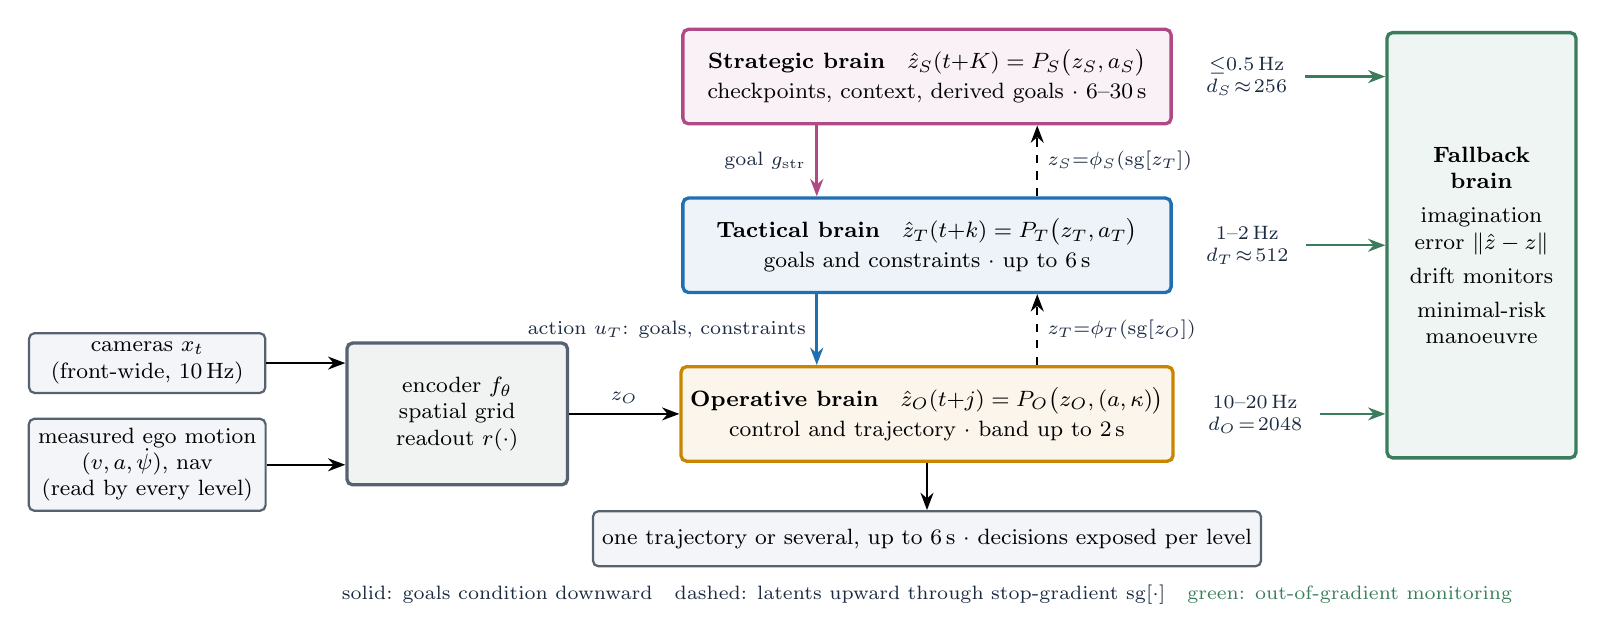
\begin{tikzpicture}[node distance=4mm and 6mm]
  % sensors and encoder
  \node[plain,minimum width=30mm] (cam) {cameras $x_t$\\(front-wide, 10\,Hz)};
  \node[plain,minimum width=30mm,below=3mm of cam] (ego) {measured ego motion\\$(v,a,\dot\psi)$, nav\\(read by every level)};
  \node[box=enc,minimum width=28mm,minimum height=18mm,right=10mm of $(cam.east)!0.5!(ego.east)$] (enc) {encoder $f_\theta$\\spatial grid\\readout $r(\cdot)$};
  \draw[arr] (cam.east) -- (enc.west|-cam.east);
  \draw[arr] (ego.east) -- (enc.west|-ego.east);
  % the three predictive brains
  \node[box=levO,minimum width=62mm,minimum height=12mm,right=14mm of enc] (O) {\textbf{Operative brain} \; $\hat z_O(t{+}j)=P_O\big(z_O,(a,\kappa)\big)$\\[0.5mm] control and trajectory $\cdot$ band up to 2\,s};
  \node[box=levT,minimum width=62mm,minimum height=12mm,above=9mm of O] (T) {\textbf{Tactical brain} \; $\hat z_T(t{+}k)=P_T\big(z_T,a_T\big)$\\[0.5mm] goals and constraints $\cdot$ up to 6\,s};
  \node[box=levS,minimum width=62mm,minimum height=12mm,above=9mm of T] (S) {\textbf{Strategic brain} \; $\hat z_S(t{+}K)=P_S\big(z_S,a_S\big)$\\[0.5mm] checkpoints, context, derived goals $\cdot$ 6--30\,s};
  \draw[arr] (enc.east) -- node[lbl,above]{$z_O$} (O.west);
  % clocks
  \node[lbl,right=3mm of S] (cS) {$\le$0.5\,Hz\\$d_S\!\approx\!256$};
  \node[lbl,right=3mm of T] (cT) {1--2\,Hz\\$d_T\!\approx\!512$};
  \node[lbl,right=3mm of O] (cO) {10--20\,Hz\\$d_O\!=\!2048$};
  % goals down (solid), latents up (dashed, stop-gradient)
  \draw[goal,levS] ([xshift=-14mm]S.south) -- node[lbl,left]{goal $g_{\mathrm{str}}$} ([xshift=-14mm]T.north);
  \draw[goal,levT] ([xshift=-14mm]T.south) -- node[lbl,left]{action $u_T$: goals, constraints} ([xshift=-14mm]O.north);
  \draw[lat] ([xshift=14mm]O.north) -- node[lbl,right]{$z_T{=}\phi_T(\mathrm{sg}[z_O])$} ([xshift=14mm]T.south);
  \draw[lat] ([xshift=14mm]T.north) -- node[lbl,right]{$z_S{=}\phi_S(\mathrm{sg}[z_T])$} ([xshift=14mm]S.south);
  % fallback brain
  \node[box=levF,minimum width=24mm,minimum height=54mm,right=27mm of T,yshift=0mm] (F) {\textbf{Fallback}\\\textbf{brain}\\[1mm]imagination\\error $\|\hat z-z\|$\\[1mm]drift monitors\\[1mm]minimal-risk\\manoeuvre};
  \draw[arr,levF] (S.east -| cS.east) ++(1mm,0) -- (F.west|-S.east);
  \draw[arr,levF] (T.east -| cT.east) ++(1mm,0) -- (F.west|-T.east);
  \draw[arr,levF] (O.east -| cO.east) ++(1mm,0) -- (F.west|-O.east);
  % output
  \node[plain,below=6mm of O,minimum width=62mm] (plan) {one trajectory or several, up to 6\,s $\cdot$ decisions exposed per level};
  \draw[arr] (O.south) -- (plan.north);
  % legend
  \node[lbl,below=1mm of plan,align=left] {\textcolor{navy}{solid: goals condition downward}\quad \textcolor{navy}{dashed: latents upward through stop-gradient $\mathrm{sg}[\cdot]$}\quad \textcolor{levF}{green: out-of-gradient monitoring}};
\end{tikzpicture}}
\caption{\textbf{The 4B architecture.} Four brains at separated clocks and horizons. Each predictive level owns its own predictor in
its own latent space, and the state shrinks while the clock slows going up ($d_S<d_T<d_O$, $\tau_S>\tau_T>\tau_O$), so upper levels
are forced to abstract. Goals condition strictly downward, through the readers and the planner cost; the predictors themselves are action-conditioned and goal-free. Latents pass upward only through stop-gradient adapters, and the
gradient-isolation matrix of \cref{eq:gmatrix} is tested on every build. The fallback brain consumes every level's imagination error
and owns the minimal-risk manoeuvre.}
\label{fig:4b}
\end{figure*}

\subsection{Levels, clocks and predictors}
Let $\ell\in\{O,T,S\}$ index the operative, tactical and strategic levels. Each level owns:
\begin{itemize}
  \item a state $z_\ell\in\Rset^{d_\ell}$;
  \item a clock $\tau_\ell$ and a horizon;
  \item an action space $a_\ell$;
  \item a predictor $P_\ell$ in its own space.
\end{itemize}
The operative state is a spatial-grid readout of the encoder, $z_O=r(f_\theta(x))$ (never a global pool). Upper states are adapters over
\emph{stopped} lower latents, $z_T=\phi_T(\mathrm{sg}[z_O])$ and $z_S=\phi_S(\mathrm{sg}[z_T])$. Each level's dynamics are conditioned on
that level's own action:
\begin{equation}
\begin{aligned}
\hat z_S(t{+}K) &= P_S\big(z_S(t),a_S(t)\big),\\
\hat z_T(t{+}k) &= P_T\big(z_T(t),a_T(t)\big),\\
\hat z_O(t{+}j) &= P_O\big(z_O(t),(a,\kappa)_t\big).
\end{aligned}
\end{equation}
Goals do not enter the predictors. They condition the lower levels through the readers and the planner cost (\cref{sec:bands}).
Two structural properties follow by construction and are then verified.

\paragraph{(1) Abstraction by down-sampling under a shrinking state.} With $d_S<d_T<d_O$ and $\tau_S>\tau_T>\tau_O$, an upper level cannot
represent lower-level detail even if its objective would reward it. At 0.2\,Hz a 15\,s strategic roll is three steps of a 256-dimensional
model (about seven at 0.5\,Hz), so only the operative path runs at the full rate.

\paragraph{(2) The gradient-isolation matrix.} Let $G[u,v]=1$ iff a gradient path from module $u$ into module $v$ is permitted. With
$\mathcal P$ the planner and goal heads and $\mathcal E$ the encoder,
\begin{equation}\label{eq:gmatrix}
G[\mathcal P,\mathcal E]=0,\quad G[\ell',\ell]=0\ \ (\ell'\text{ above }\ell),\quad G[\ell,\ell]=1 .
\end{equation}
Every build checks it by asserting zero gradient on forbidden paths, with a deliberate-regression arm that must fail.

\subsection{Time bands, the current ego state and the tactical action}\label{sec:bands}
Let $\Delta=0.2$\,s be the grid step and $t$ the present. The levels own the bands
\begin{equation}
B_O=(0,2]\,\mathrm{s},\quad B_T=(2,6]\,\mathrm{s},\quad B_S=(6,30]\,\mathrm{s}.
\end{equation}
The output of the stack is one trajectory or several, up to 6\,s,
\begin{equation}
X_t=\big(x_{t+j\Delta}\big)_{j=1}^{30}\in\Rset^{30\times2},
\end{equation}
so knots 1--10 lie in $B_O$ and knots 11--30 in $B_T$. A horizon of 0.8\,s is not a long-term abstract level: a level's reach has to
match its band.

\paragraph{The cascade.} Let $e_t$ be the current measured ego state, including yaw rate, and $V_t$ the vision tokens of the current and
past frames, with the navigation command and speed limit. Every level reads $e_t$, and no level reads a state planned by another level:
\begin{equation}\label{eq:cascade}
\begin{aligned}
s_t&=f_S(e_t,V_t),\\
u_t&=f_T(e_t,V_t,\hat s),\\
X_t&=f_O(e_t,V_t,\hat s,\hat u),
\end{aligned}
\end{equation}
where a hat marks a held output re-expressed in the current ego frame by measured odometry. The tactical output is a \emph{tactical
action},
\begin{equation}
u_t=(g_t,\lambda^{\mathrm{lat}}_t,\lambda^{\mathrm{lon}}_t,\gamma_t),
\end{equation}
the goals, the lateral and longitudinal classes and the constraints, over a horizon of up to 6\,s. T has no trajectory head. $u_t$
conditions O as its action, so the plan is a function of the context \emph{given} $u_t$. A single decoder produces all 30 knots, which
makes the plan continuous across 2\,s by construction, and the two bands differ only in the loss:
\begin{equation}
\mathcal L_O=w_{\mathrm{op}}\,\ell\big(X^{1:10},X^{\ast\,1:10}\big)+w_{\mathrm{tac}}\,\ell\big(X^{11:30},X^{\ast\,11:30}\big).
\end{equation}
For $M$ hypotheses, $X^{(m)}_t=f_O(\,\cdot\mid\hat u^{(m)})$ with $\hat u^{(m)}$ the $M$ best tactical actions; $M=1$ is the arm of record.

\paragraph{The strategic level.} Its output is $\sigma_t=(C_t,p_t,\gamma^S_t)$: checkpoints $C_t$ at $\tau\in\{6,9,\dots,30\}$\,s; the
posteriors $p_t$ of the detected context (country, period of day, illumination, weather, visibility and road surface), read from the
current and past images only; and the goals $\gamma^S_t$ derived from them. $\sigma_t$ enters $f_T$ as a detached input, so strategic goals
reach O through $u_t$. No output of a situation classifier enters any goal path.

\paragraph{World-model planning.} The levels $l=1,2,3$ step at $\tau_l=0.2,0.6,3.0$\,s and are trained to reaches of 2, 6 and 18\,s. Following
H-JEPA~\cite{hjepa}, with $g$ a goal latent, $\tilde z^{\,l+1}_i$ the rollout of level $l$ lifted to the level above, and $l=2,1$,
\begin{equation}
\begin{aligned}
a^{3,\ast}&=\arg\min_{a^3}\big\|\hat z^{\,3}_{T_3}-g\big\|^2,\\
a^{l,\ast}&=\arg\min_{a^l}\big\|\tilde z^{\,l+1}_{K}-\hat z^{\,l+1,\ast}_{K}\big\|^2\\
&\qquad+\lambda\sum_{i<K}\big\|\tilde z^{\,l+1}_{i}-\hat z^{\,l+1,\ast}_{i}\big\|^2 .
\end{aligned}
\end{equation}
Each level plans from its own encoded current state, and the only downward signal is the predicted state of the level above. This
planner is the baseline against which other approaches are compared.

\paragraph{Status.} \Cref{eq:cascade} is trained on v8F-mini as described in \cref{sec:v8f}, with equal knot weights and tactical labels
over 2--8\,s. The band losses, the 2--6\,s labels, the strategic extension and the world-model planner are built and tested, and the
world models for these bands are in training. A first planner read on the earlier models, with a true-future goal (T0), did not beat
holding the action. No driving result exists yet for this design; the reads of \cref{sec:results} are diagnostics on logged frames, and \cref{sec:status} states what has been read since and what is running.

\subsection{Self-supervised world-model objective}
The programme's world model is trained without perception labels, without HD maps and without reward. Its objective is
\begin{equation}
\begin{aligned}
\mathcal L={}&\mathcal L_{\mathrm{pred}}+\lambda_{\mathrm{tac}}\mathcal L_{\mathrm{tac}}+\lambda_{\mathrm{sig}}\big(\mathcal S(Z)+\mathcal S(\hat Z)\big)\\
&+\lambda_{\mathrm{inv}}\mathcal L_{\mathrm{inv}}+\lambda_{\mathrm{im}}\mathcal L_{\mathrm{imag}} .
\end{aligned}
\end{equation}
\paragraph{Residual multi-horizon prediction.} $\hat z_{t+k}=z_t+\Delta_k(z_{t-W+1:t},a_{t-W+1:t})$, scored by a \emph{change-weighted}
error with per-dimension weights $w\propto|z_{t+k}-z_{t+k-1}|$ normalised to unit mean. On driving data only 5--11\,\% of a frame
changes per step, so the weighting puts the gradient where the consequences are.

\paragraph{Provable anti-collapse.} $\mathcal S(\cdot)$ is the sliced Epps--Pulley statistic of LeJEPA~\cite{lejepa}. Embeddings are
projected onto $M$ fresh unit directions, and each projection $Y$ (a sample of size $n$) is tested against $\mathcal N(0,1)$:
\begin{equation}
T_{n,\beta}=\tfrac1n\!\sum_{j,k}e^{-\frac{\beta^2(Y_j-Y_k)^2}{2}}-\tfrac{2}{\sqrt{1+\beta^2}}\sum_j e^{-\frac{\beta^2Y_j^2}{2(1+\beta^2)}}+\tfrac{n}{\sqrt{1+2\beta^2}} .
\end{equation}
By the Cram\'er--Wold theorem, standard normal one-dimensional projections in all directions imply a joint standard Gaussian, the
embedding law LeJEPA shows to be optimal; $M$ random directions test this only approximately. The gradients stay uniformly bounded~\cite{lejepa}.

\paragraph{Inverse dynamics.} $\mathcal L_{\mathrm{inv}}=\|g(z_t,z_{t+1})-a_t\|^2$ uses proprioception as free supervision and forces
controllable state into the latent.

\paragraph{Imagination of unobserved areas.} Masked sectors evolve by semi-Lagrangian advection under a learned flow,
$\hat z_{t+1}(u)=z_t(u-v_\theta(u)\Delta t)$, refined by attention, with a per-cell log-variance $s(u)$:
\begin{equation}
\mathcal L_{\mathrm{imag}}=\sum_u w(u)\Big[e^{-s(u)}\tfrac{\|\hat z(u)-z(u)\|^2}{2}+\tfrac{s(u)}{2}\Big],
\end{equation}
with $w=1$ on hidden cells and 0.1 on visible ones. The model must know \emph{where it cannot know}. The variance field is the
world-model-native trigger for sensor steering and for the fallback brain.

\subsection{Why a hierarchy is data-efficient}
Two arguments motivate the factorisation~\cite{hplwm,ssshashua}.
\begin{enumerate}[label=(\roman*)]
  \item \textbf{Horizon.} Planning regret in learned models grows with the horizon, so a short per-level horizon has a smaller bound at
        that level. Summed over the levels, equal per-step errors give the undivided bound back: the gain requires the coarser levels
        to carry a smaller per-step error, which is an empirical question.
  \item \textbf{Recombination.} If a driving situation is a combination of a place $p\in\mathcal P$, a manoeuvre $m\in\mathcal M$ and a
        control profile, a flat learner must cover $|\mathcal P|\cdot|\mathcal M|$ combinations. A hierarchy that learns each level
        separately covers roughly $|\mathcal P|+|\mathcal M|$, provided places and manoeuvres combine independently.
\end{enumerate}

\subsection{Fallback and self-knowledge}
The relative imagination error $\|\hat z_t-z_t\|$ is a free, always-on familiarity signal. Layered monitors arm a deterministic
minimal-risk manoeuvre:
\begin{itemize}
  \item imagination error at 10\,Hz;
  \item routing statistics at 1\,Hz;
  \item Mahalanobis drift at 0.1\,Hz.
\end{itemize}
Their logs are the substrate for the ISMR/DSSAD incident-reporting requirements: self-monitoring \emph{is} the evidence trail.

The programme's 263\,M-parameter 4B flagship was its first arm to beat the kinematic floor in open loop: ADE@2\,s 0.452\,m against
0.500\,m for the best of three kinematic models and 0.523\,m for CTRV. On windows where kinematics diverge from the realised future, it
beat CTRV by 0.80\,m, and the whole of that advantage came from vision.

% =====================================================================================================================
\section{v8F-mini: a typed reference implementation}\label{sec:v8f}

\begin{figure*}[t]
\centering
\resizebox{0.98\textwidth}{!}{%
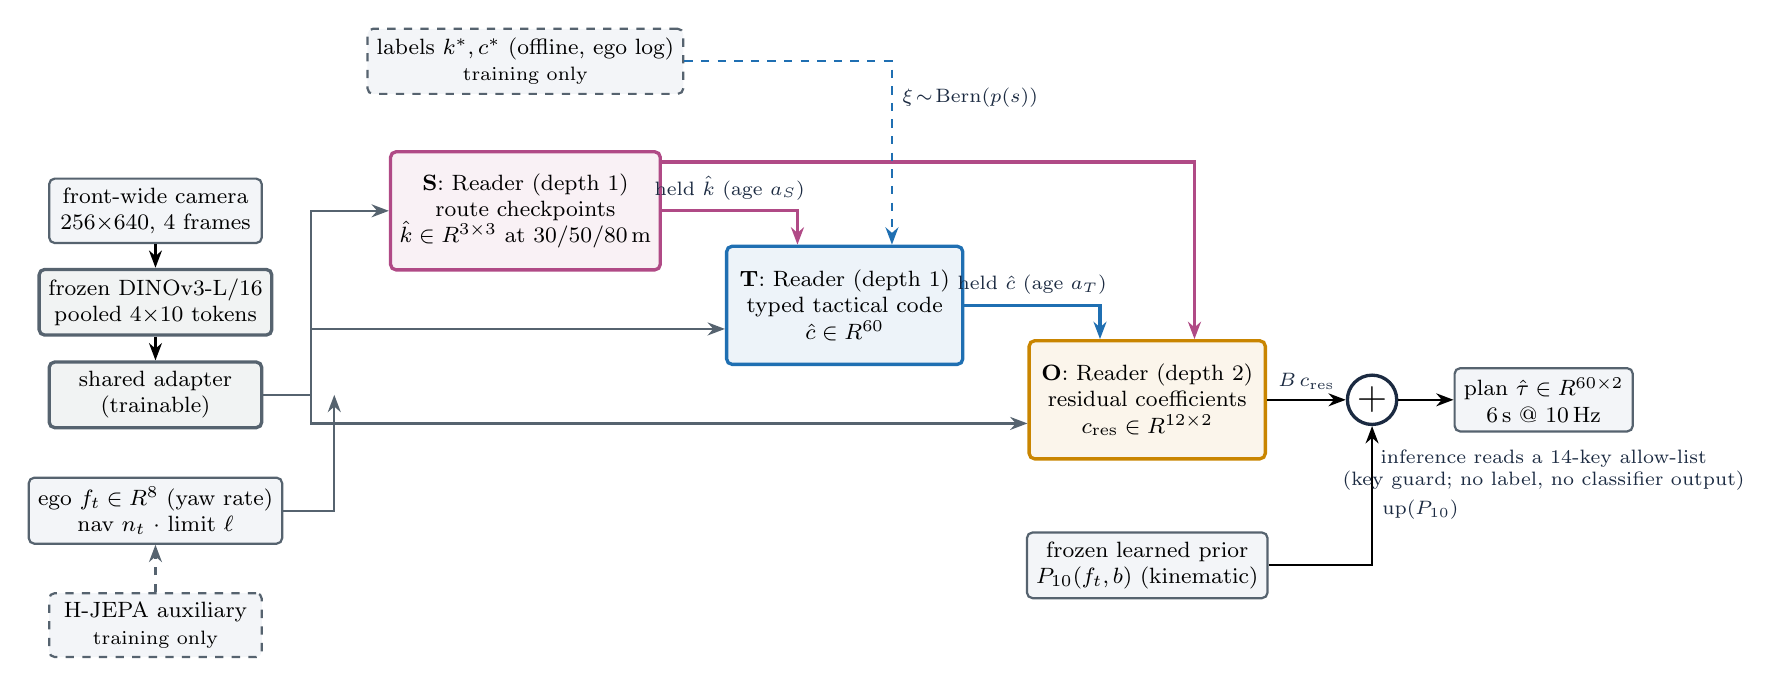
\begin{tikzpicture}[node distance=5mm and 7mm]
  % inputs
  \node[plain,minimum width=27mm] (img) {front-wide camera\\256$\times$640, 4 frames};
  \node[box=enc,minimum width=27mm,below=3mm of img] (dino) {frozen DINOv3-L/16\\pooled $4{\times}10$ tokens};
  \node[box=enc,minimum width=27mm,below=3mm of dino] (adp) {shared adapter\\(trainable)};
  \node[plain,minimum width=27mm,below=6mm of adp] (ego) {ego $f_t\in\Rset^8$ (yaw rate)\\nav $n_t$ $\cdot$ limit $\ell$};
  \draw[arr] (img) -- (dino); \draw[arr] (dino) -- (adp);
  % readers
  \node[box=levS,minimum width=30mm,minimum height=15mm,right=16mm of img] (S) {\textbf{S}: Reader (depth 1)\\route checkpoints\\$\hat k\in\Rset^{3\times3}$ at 30/50/80\,m};
  \node[box=levT,minimum width=30mm,minimum height=15mm,right=8mm of S,yshift=-12mm] (T) {\textbf{T}: Reader (depth 1)\\typed tactical code\\$\hat c\in\Rset^{60}$};
  \node[box=levO,minimum width=30mm,minimum height=15mm,right=8mm of T,yshift=-12mm] (O) {\textbf{O}: Reader (depth 2)\\residual coefficients\\$c_{\mathrm{res}}\in\Rset^{12\times2}$};
  \coordinate (bus) at ($(adp.east)+(6mm,0)$);
  \draw[thick,enc] (adp.east) -- (bus);
  \draw[arr,enc] (bus) |- (S.west);
  \draw[arr,enc] (bus) |- ([yshift=-3mm]T.west);
  \draw[arr,enc] (bus) |- ([yshift=-3mm]O.west);
  \draw[arr,enc] (ego.east) -| ([xshift=3mm]bus);
  % held outputs flow down the hierarchy
  \draw[goal,levS] (S.east) -| node[lbl,above,pos=0.25]{held $\hat k$ (age $a_S$)} ([xshift=-6mm]T.north);
  \draw[goal,levT] (T.east) -| node[lbl,above,pos=0.25]{held $\hat c$ (age $a_T$)} ([xshift=-6mm]O.north);
  \draw[goal,levS] ([yshift=-1.5mm]S.north east) -| ([xshift=6mm]O.north);
  % prior and sum
  \node[plain,minimum width=30mm,below=9mm of O] (P10) {frozen learned prior\\$P_{10}(f_t,b)$ (kinematic)};
  \node[circle,draw=navy,very thick,inner sep=1.2pt,right=10mm of O] (sum) {\Large$+$};
  \node[plain,right=7mm of sum,minimum width=22mm] (tau) {plan $\hat\tau\in\Rset^{60\times2}$\\6\,s @ 10\,Hz};
  \draw[arr] (O.east) -- node[lbl,above]{$B\,c_{\mathrm{res}}$} (sum.west);
  \draw[arr] (P10.east) -| node[lbl,right,pos=0.7]{$\mathrm{up}(P_{10})$} (sum.south);
  \draw[arr] (sum.east) -- (tau.west);
  % training-only components
  \node[plain,dashed,minimum width=30mm,above=7mm of S] (lab) {labels $k^\ast,c^\ast$ (offline, ego log)\\\scriptsize training only};
  \draw[lat,levT] (lab.east) -| node[lbl,right,pos=0.6]{\scriptsize $\xi\!\sim\!\mathrm{Bern}(p(s))$} ([xshift=6mm]T.north);
  \node[plain,dashed,minimum width=27mm,below=6mm of ego] (wm) {H-JEPA auxiliary\\\scriptsize training only};
  \draw[lat,enc] (wm.north) -- (ego.south);
  % guard
  \node[lbl,below=1mm of tau,align=center] (guard) {\textcolor{navy}{inference reads a 14-key allow-list}\\\textcolor{navy}{(key guard; no label, no classifier output)}};
\end{tikzpicture}}
\caption{\textbf{v8F-mini.} Three learned readers over frozen DINOv3 features and a shared trainable adapter. S emits route checkpoints,
T a typed 60-dimensional tactical code, and O the coefficients of a ramped cosine basis added to a \emph{frozen} learned kinematic
prior. Upper outputs are \emph{held} with quantised ages and re-expressed in the current frame by odometry. Labels enter only through
scheduled teacher forcing in training. Inference reads a fixed allow-list of inputs, enforced by a key guard.}
\label{fig:v8f}
\end{figure*}

\subsection{Inputs and notation}
Time runs on a 0.2\,s grid. For a window ending at $t$, the model reads:
\begin{itemize}
  \item \textbf{scene tokens} $z_{t'}\in\Rset^{40\times1024}$, frozen DINOv3-L/16 features of the cylindrical front-wide frame, pooled to a
        $4\times10$ grid, four frames per layer;
  \item \textbf{ego features} $f_t=(v,a,\kappa,v^2,va,v\kappa,v^2\kappa,a\kappa)$, with curvature $\kappa$ from the \emph{measured yaw rate}
        (never a steering angle);
  \item \textbf{a navigation command} $n_t$;
  \item \textbf{a speed bucket} $\ell$;
  \item \textbf{measured odometry} between frames.
\end{itemize}
The output is a 6\,s plan $\tau\in\Rset^{60\times2}$ in the ego frame, scored on its 30 knots at 0.2\,s. Several plans are possible,
one per top tactical hypothesis; the arm reported here emits one.

\subsection{The S/T/O decomposition}
S ticks at about 1\,Hz, T at about 2\,Hz and O at 10\,Hz. On the cache grid the model uses sample-and-hold with quantised ages:
\begin{itemize}
  \item T last ticked $a_T\in\{0,1,2\}$ steps ago;
  \item S ticked $u\le4$ steps before T, so $a_S=a_T+u$.
\end{itemize}
With $t_T=t-a_T$ and $t_S=t-a_S$,
\begin{equation}
\begin{aligned}
\hat k&=f_S\big(z_{t_S},f_{t_S},n_{t_S},\ell\big),\\
\hat c&=f_T\big(z_{t_T},f_{t_T},n_{t_T},\ell,\Pi_{t_S\to t_T}\hat k\big),\\
\hat\tau&=f_O\big(z_t,f_t,n_t,\ell,\Pi_{t_S\to t}\hat k,\hat c,(a_T,a_S)\big),
\end{aligned}
\end{equation}
where $\Pi_{a\to b}$ re-expresses held checkpoints from frame $a$ to frame $b$ by odometry. The conditioning sets are strictly nested,
$\mathrm{in}(S)\subset\mathrm{in}(T)\subset\mathrm{in}(O)$. Information flows between levels only through \emph{held outputs}, never
through shared hidden state. Each level reads the measured ego state of its own tick, and no level reads a state planned by another
level. Each $f_\ell$ is a \emph{Reader}: four learned queries cross-attend to the conditioning and scene tokens
through a pre-norm transformer decoder, followed by an MLP head.

\subsection{The tactical code as a typed interface}
\begin{equation}
\begin{aligned}
c=\big[\,&\underbrace{\sigma(g)}_{22\text{ goals}}\;\big|\;\underbrace{\mathrm{softmax}(\lambda_{\mathrm{lat}})}_{5}\;\big|\\
&\underbrace{\mathrm{softmax}(\lambda_{\mathrm{lon}})}_{7}\;\big|\;\underbrace{(\gamma-\mu)/\sigma_{\mathrm{cons}}}_{26\text{ constraints}}\,\big]\in\Rset^{60}.
\end{aligned}
\end{equation}
The 26 constraint cells cover turn timing and geometry, longitudinal target speeds and reach times, the stop point, the lead gap and
time gap, and the speed band. The code is the tactical action of \cref{sec:bands}: T emits goals and constraints, has no trajectory
head, and $\hat c$ conditions O. The route checkpoints of this arm sit at 30, 50 and 80\,m, with a median arrival of 3, 5 and 8\,s, so
they do not yet cover the strategic band in seconds; \cref{sec:bands} gives the extension.

\paragraph{An information-theoretic reading.} Ground-truth codes $C^\ast=g(Y)$ are deterministic functions of the human future $Y$, so the
data-processing inequality gives $I(C;Y)\ge I(C;C^\ast)$. Supervised agreement with $C^\ast$ is therefore a lower-bound proxy for
informativeness about the future. O also reads the scene, so the code is a \emph{typed side channel}, not a strict bottleneck, and its
usage is measurable by intervention (\cref{sec:results}).

\subsection{Trajectory as an exact residual on a kinematic prior}
Let $P=P_{10}(f_t,b)\in\Rset^{30\times2}$ be a \emph{frozen} learned prior: a damped base path re-timed by constant acceleration, plus an
eight-feature MLP fitted once. Let $\mathrm{up}$ interpolate it to 0.1\,s. The plan is
\begin{equation}\label{eq:traj}
\tau=\mathrm{up}\big(P_{10}(f_t,b)\big)+B\,c_{\mathrm{res}},\quad B_{ik}=\tfrac{i+1}{N}\cos\!\Big(\tfrac{k\pi(i+\frac12)}{N}\Big),
\end{equation}
with $N=60$, $k=0,\dots,11$, $c_{\mathrm{res}}=s\cdot\mathrm{MLP}(h_O)$, $s=2$\,m, and the last layer zero-initialised.

\begin{proposition}[Floor identity, ramp and band limit]\hfill
\begin{enumerate}[label=(\alph*)]
  \item \textbf{Floor identity.} $c_{\mathrm{res}}=0$ implies $\tau=\mathrm{up}(P_{10})$ exactly, so the untrained model \emph{is} the prior.
  \item \textbf{Ramp.} $|B_{ik}|\le(i+1)/N$, so the residual vanishes linearly as $t\to0$ and the plan starts at the prior's origin.
  \item \textbf{Band limit.} With $k\le11$ the cosine factor has at most eleven half-cycles over 6\,s, below 1\,Hz, and the linear ramp
        modulates it smoothly: a smooth adjustment, while the prior carries the kinematics.
\end{enumerate}
\end{proposition}
Every learned metre is thus measured against the floor it must beat. Each property is pinned by a unit test with a mutation check.

\subsection{Losses and scheduled teacher forcing}
The training loss is
\begin{multline}
\mathcal L=w_{\mathrm{ck}}\mathcal L_{\mathrm{ck}}+w_{\mathrm{tac}}\big(\mathcal L_{\mathrm{goal}}+\tfrac12(\mathcal L_{\mathrm{lat}}+\mathcal L_{\mathrm{lon}})+w_{\mathrm{cons}}\mathcal L_{\mathrm{cons}}\big)\\
+w_{\mathrm{traj}}\big(\tfrac13\mathcal L_{\ADE}+\tfrac1{12}\mathcal L_{\mathrm{FDE}}\big)+w_{\mathrm{pen}}\textstyle\sum_r\rho_r+w_{\mathrm{wm}}\mathcal L_{\mathrm{wm}}.
\end{multline}
Its terms:
\begin{itemize}
  \item \textbf{partial-label cross-entropies} $-\log\sum_{c\in\mathcal A}p_c$ handle the sets of allowed manoeuvres;
  \item \textbf{constraint cells} use a masked Huber loss;
  \item \textbf{rule penalties} $\rho_r$ (speed, stop, turn, lead) are differentiable hinges that are positive \emph{iff} a frozen rule reports a
        violation;
  \item \textbf{the world-model auxiliary} $\mathcal L_{\mathrm{wm}}$ is an H-JEPA objective on the shared adapter~\cite{hjepa}.
\end{itemize}
During training, O and T read a mixture of predicted and ground-truth upper outputs,
\begin{equation}
\begin{gathered}
\tilde c=\xi_c\,c^\ast+(1-\xi_c)\,\hat c,\qquad \xi_c\sim\mathrm{Bernoulli}\big(p(s)\big),\\
p(s)=1-0.8\min(s/S,1),
\end{gathered}
\end{equation}
which anneals the share of ground truth from 1.0 to 0.2~\cite{schedsamp}. At inference $\xi\equiv0$, and labels are never read.

\subsection{Admissibility by construction}
\begin{itemize}
  \item Inference reads a fixed allow-list of 14 keys. A key guard records every access during the forward pass, and a test proves
        that a deliberately peeking model is caught.
  \item The goal path may not contain the output of any situation classifier.
  \item Labels may use the ego future, but inference may not.
\end{itemize}

% =====================================================================================================================
\section{Mathematical background}\label{sec:math}

\subsection{Plug-in composition and propagated interface error}
By the chain rule, $p(y\mid x)=\sum_{k,c}p(k\mid x)\,p(c\mid x,k)\,p(y\mid x,k,c)$. Factorisation alone is an identity; its value lies in
\emph{supervision structure}. Each factor is fitted against its own offline target, and inference is a plug-in composition
$\hat y=\mu_O(x,\hat k,\hat c)$.
\begin{proposition}[Error decomposition]\label{prop:lip}
If $\mu_O$ is $L_k$- and $L_c$-Lipschitz in its code arguments, then
\begin{equation}
\begin{aligned}
\|\hat y-y\|\le{}&\underbrace{\|\mu_O(x,k^\ast,c^\ast)-y\|}_{\textup{oracle term}}\\
&+L_c\|\hat c-c^\ast\|+L_k\|\hat k-k^\ast\| .
\end{aligned}
\end{equation}
\end{proposition}
\noindent The oracle term is measurable by substituting ground-truth codes. The gap between the model's own code and the oracle is
the propagated interface error, and it is the headroom the hierarchy offers (\cref{sec:results}).

\subsection{Convex response to tactical accuracy}
Define the partial substitution $\hat c_\alpha=\hat c+\alpha(c^\ast-\hat c)$ on the 26 constraint cells, and the recovered fraction
\begin{equation}
r(\alpha)=\frac{\ADE(\hat c)-\ADE(\hat c_\alpha)}{\ADE(\hat c)-\ADE(\hat c_1)} .
\end{equation}
Linear response gives $r(\alpha)=\alpha$. We measure $r(0.25)=0.08$--$0.16$, $r(0.5)=0.20$--$0.36$ and $r(0.75)=0.48$--$0.73$. The
response is \emph{convex}: O is flat near its own code and steep near the truth. The value of tactical accuracy therefore compounds,
and the last metres of tactical precision buy the most driving.

\subsection{Interface support and exposure bias}
Whole-code teacher forcing trains O on the two-point mixture $p\,\delta_{c^\ast(x)}+(1-p)\,\delta_{\hat c(x)}$. A partial code
$c_u=(c^\ast_u,\hat c_{\bar u})$ lies off that support, so its response is unconstrained by the training loss. The remedy is to widen
the support: draw an independent $\xi_u$ per unit of the code at the same marginal $p(s)$,
\begin{equation}
\tilde c_u=\xi_u c^\ast_u+(1-\xi_u)\hat c_u,\qquad \xi_u\stackrel{\mathrm{iid}}{\sim}\mathrm{Bern}\big(p(s)\big).
\end{equation}
This keeps each cell's marginal unchanged while covering $2^7$ corners per window instead of 2.

The same logic applies along time. A policy trained only on expert states incurs compounding error of order $\varepsilon T^2$, while
on-policy aggregation (DAgger~\cite{dagger}) reduces it to order $\varepsilon T$ under that reduction's no-regret assumptions. v8F-mini realises this by replacing 10\,\% of the
training samples with the model's \emph{own rolled-out states}, labelled from the human future.

\subsection{Estimator theory: three variances, one interval}
Windows are grouped into $M=141$ episodes. For arms $a,b$ the point estimate is the full-set mean difference
$\hat\Delta=\frac1N\sum_w[d_a(w)-d_b(w)]$. The paired episode-cluster bootstrap resamples episodes with replacement, using the same
draw for both arms, and reports percentile intervals. By the law of total variance, with training randomness $\theta$, inference
randomness $\omega$ and the episode draw $E$,
\begin{equation}
\begin{aligned}
\mathrm{Var}(\hat\Delta)={}&\underbrace{\mathrm{Var}_\theta\,\mathbb E[\hat\Delta\mid\theta]}_{\text{training seeds}}+\underbrace{\mathbb E_\theta\mathrm{Var}_\omega\,\mathbb E_E[\hat\Delta\mid\theta,\omega]}_{\text{inference}}\\
&+\underbrace{\mathbb E_{\theta,\omega}\mathrm{Var}_E[\hat\Delta\mid\theta,\omega]}_{\text{episodes}} .
\end{aligned}
\end{equation}
The bootstrap estimates the episode term only. TanitAD therefore reports the seed term separately, through two training seeds and a
pre-registered floor $F=|\Delta_{s_0}-\Delta_{s_1}|$ with bar $2F$. For a deterministic forward pass the inference term is exactly zero,
and the programme verifies that on re-evaluation (maximum per-window deviation 0.0\,m).

% =====================================================================================================================
\section{A machine-checked theory of the hierarchy}\label{sec:theory}
The design claims of \cref{sec:4b} can be stated as theorems about model classes. Each has a premise that must be \emph{measured}
before it says anything about a model. We wrote nine such statements (T1--T9, \cref{tab:theory}) and froze each before its proof.
All were checked by machine: 56 verification conditions with the SMT solver Z3, each family with mutated twins that the solver must
refute (30 are), and the central ones in general form with the Lean~4 kernel and Mathlib (72 theorems in three files, no \texttt{sorry}, standard
axioms only). Two groups were written after reads they explain; for those reads they are explanatory, not predictive. The premises
are tested in \cref{sec:premises}.

\begin{table*}[!tp]
\centering
\caption{\textbf{Nine statements, their machine check, and their measured premise for v8F-mini.} Z3: verification conditions proved by
an SMT solver, with mutated twins refuted. Lean: checked by the Lean~4 kernel in general form. Every measured value is a \tier{T0} or
\tier{T1-kin} diagnostic on logged frames (seed 0 / seed 1 where two values are given).}
\label{tab:theory}
\small
\begin{tabularx}{\textwidth}{@{}l>{\raggedright\arraybackslash}p{60mm}l>{\raggedright\arraybackslash}X@{}}
\toprule
 & Statement & Check & Measured premise or consequence for v8F-mini \\
\midrule
T1 & A level that jumps $k$ steps has the better worst-case bound at every horizon iff $\varepsilon_k<\varepsilon\sum_{i<k}L^i$ & Z3, Lean &
holds in the linear class: the direct 2\,s error is 0.42/0.43 of ten one-step errors; the learned ten-step rollout fails (skill $-0.15$/$-0.17$ at 2\,s) \\
T2 & Under squared error no plan beats the mean; under a hit-or-miss criterion a decided plan beats every single plan iff selection accuracy exceeds the share of the larger mode & Z3, Lean &
premise open (top-1 selection 57--59\,\%); measured at six seeds: hierarchy ahead under the primary protocol ($-0.09$\,m on all windows, six of six seeds), not established from scratch \\
T3 & A shield keeps a rule for every network; a penalty of weight $\lambda$ only bounds the violation by $(J_0-J_\infty)/\lambda$ & Z3, Lean &
with the logged rest distance: overrun exactly 0 and stop-window 2--6\,s ADE $-3.51$/$-3.37$\,m; with the model's own stop cue: no gain \\
T4 & Class weighting is a threshold move, $\tau=r/(1+r)$ & Z3 &
one added bias reproduces the stop decision of a class-weighted training run in 4 of 4 cells \\
T5 & A state pooled over cells keeps counts and totals and loses position and motion & Z3, Lean &
planted object: AUROC 1.00 from a grid state, 0.50 from the mean state; trained state: lead presence $+0.21$/$+0.19$ AUROC beyond ego motion, change of the gap: nothing beyond ego motion; a state that keeps the cell layout reads the lead gap at $R^2$ 0.55/0.54 against 0.24/0.21 \\
T6 & Skill over persistence is the predictable fraction of the change & Z3 &
the learned world model is below a closed-form ridge at 0.2\,s and at 2\,s; a closed-form stack of both is above both at every horizon \\
T7 & An imagined gain is a real gain only above twice the model gap & Z3, Lean &
not yet admissible for objects: the mean state decodes to the scene gist; the grid state holds the lead, but no learned rollout yet reads it better than a copy of the present state at 2\,s \\
T8 & Sampling by gradient norm minimises the second moment of the weighted gradient & Z3 &
selection by coverage or by leverage lands inside the range of random draws (probe level); trained arms: a quarter of the clips shows no measured cost (preliminary) \\
T9 & A member average is never worse than the member mean; a rank-one edit is the least change that moves one key & Z3, Lean &
a two-member weight average realises 0.74 of the ensemble gain in one forward pass \\
\bottomrule
\end{tabularx}
\end{table*}

\subsection{When multi-level prediction dominates}
Let a one-step predictor have error at most $\varepsilon$ and let the dynamics expand an error by at most the factor $L\ge0$ per
step, so that $e_{t+1}\le L\,e_t+\varepsilon$ with $e_0=0$.
\begin{proposition}[Composed bound, jump bound and criterion]\label{prop:jump}
After $H$ steps $e_H\le\varepsilon\sum_{i<H}L^{i}$, and the bound is attained. A level that predicts $k$ steps at once with error
$\varepsilon_k$ has error at most $\varepsilon_k\sum_{j<m}L^{kj}$ after $m$ jumps. At every horizon $H=mk$ with $m\ge1$, the jump bound
is below the composed bound if and only if
\begin{equation}
\varepsilon_k<\varepsilon\sum_{i<k}L^{i}\qquad(\text{for }L=1:\ \varepsilon_k<k\,\varepsilon).\label{eq:jump}
\end{equation}
\end{proposition}
\noindent The horizon drops out. A slow level earns its place exactly when its direct $k$-step error is below $k$ composed fast
steps. This is the formal content of the clocks of \cref{sec:4b}, and its premise is a ratio one can measure.

\subsection{When a decision before the trajectory dominates}
\begin{proposition}[Risk split and non-dominance]\label{prop:split}
Let outcomes $y_i$ carry weights $w_i\ge0$ and modes $g(i)$ with weighted means $\mu_g$. For any plan $c$ that is constant on each mode,
\begin{equation}
\begin{aligned}
\sum_i w_i\|y_i-c_{g(i)}\|^2={}&\sum_i w_i\|y_i-\mu_{g(i)}\|^2\\
&+\sum_i w_i\|\mu_{g(i)}-c_{g(i)}\|^2 .
\end{aligned}
\end{equation}
Under squared error no single plan beats the mean, so a selector that reads only what the flat model reads cannot gain.
\end{proposition}
\noindent A hierarchy therefore pays through three channels only: (a) supervised intermediate labels, which a flat regressor never
sees; (b) an acceptance region that is not convex; (c) inputs that enter at the upper level, such as navigation. Channel (b) has an
exact form.
\begin{proposition}[Dominance under a hit-or-miss criterion]\label{prop:dom}
Let the outcomes of one context fall into two modes with centres $a$ and $b$, each outcome within $r$ of its centre, and let a plan hit
an outcome when it lies within $\mathrm{tol}\ge r$ of it. If $\|a-b\|>2\,\mathrm{tol}+2r$, all outcomes that any single plan hits lie in
one mode. A plan decided by a selector hits every outcome whose mode was selected correctly. Hence, if the selector is right on more
outcomes than the larger mode holds, the decided plan hits strictly more outcomes than every single plan.
\end{proposition}
\noindent This is the dominance claim of the programme in its exact, conditional form. Its premise is a selection accuracy above the
share of the larger mode, at a mode separation above $2\,\mathrm{tol}+2r$. Where the premise fails the theorem is silent, and a flat
plan can be ahead. The literature gives the same caution from the empirical side: most of the benefit of hierarchy in reinforcement
learning has been attributed to exploration~\cite{nachum19}, which offline imitation does not have, and acting through a goal
representation costs a bounded amount that grows with the error the representation induces~\cite{nachum18}. A flat control at matched
budget is therefore not optional.

A commit rule that hands control to the hierarchy only on flagged contexts has an exact break-even. Let $p$ be the share of
selection-critical contexts, $d_c<0<d_b$ the class means of hierarchy minus flat, and $t$ and $f$ the flag rates on the two classes.
With $s=(1-p)\,d_b/(p\,|d_c|)$, the composite beats the flat plan if and only if $t>s f$, and beats the hierarchy if and only if
$1-t<s\,(1-f)$. A flag without information cannot beat both.

\subsection{What a pooled state can hold}
The level-1 state of v8F-mini's world model is a mean over the $4\times10$ cells of adapted camera features.
\begin{proposition}[Pooling]\label{prop:pool}
Let $z=w\sum_{i\in K}(Ax_i+b_i)$ pool per-cell features $x_i$ over a set of cells $K$, with $A$ linear and $b_i$ a constant per cell.
Moving an object of feature $s$ between two cells of $K$ leaves $z$ unchanged, for every background. Moving it across the border of
$K$ changes $z$ by $wAs$. Consequently, for an object equally likely in each cell of $K$, every decoder of $z$ predicts every function
of the object's position with squared error at least the variance of that function: its skill is at most zero. With $m$ objects of
equal strength, $z$ depends on $m$ only. For any per-cell map, linear or not, a permutation of the cells leaves $z$ unchanged.
\end{proposition}
\noindent A mean over cells therefore keeps counts and totals (how many objects, the light level, how much of the frame is occupied)
and loses position and motion. An object that moves between cells changes nothing in the state, a copy predicts the next state
exactly, and a learned predictor of that state has nothing to imagine about the object. A state that keeps the cell layout reads the
position linearly, with a margin that does not depend on the background. Pooling at an intermediate scale loses position inside a
block and keeps it across blocks.

\subsection{Rules, class weights, imagination and weight space}
\begin{itemize}
  \item \emph{Rules (T3).} With a braking distance $B$ that obeys $B(v)=v\,\Delta t+B(\max(v-q,0))$, a stop-line shield preserves
        $B(v)\le d$ for \emph{any} proposed speed, its fallback is always feasible, and the distance to the line never goes below
        zero. A masked selection over candidates is admissible whenever any candidate is. A penalty of weight $\lambda$ only bounds
        the violation by $(J_0-J_\infty)/\lambda$, so a loss term guarantees nothing. What remains is perception: a shield on a
        predicted constraint violates the true rule at most as often as the constraint's envelope misses.
  \item \emph{Class weights (T4).} Under a pure prior change, deciding at 0.5 after weighting equals deciding at
        $\tau=r/(1+r)$ before weighting, with $r$ the odds ratio of the two priors. A class weight moves a threshold along one ROC
        curve and adds no discrimination.
  \item \emph{Yardstick (T6).} Skill over persistence equals the predictable fraction of the change. A feature with lag correlation
        $\rho$ gives its own past a skill of $(1-\rho)/2$, so a slowly varying pooled target leaves little to predict at short
        horizons.
  \item \emph{Imagination (T7).} If imagined and true returns differ by at most $G$, an imagined gain above $2G$ is a real gain, and
        choosing by imagined cost loses at most $2G$. This is the deterministic finite-horizon analogue of the model-based bound
        of~\cite{mbpo}; $G$ follows from \cref{prop:jump}.
  \item \emph{Data and weights (T8, T9).} Sampling in proportion to the per-sample gradient norm minimises the second moment of
        the importance-weighted gradient. The mean of $K$ members has an error equal to the mean member error minus the mean member
        scatter, so it is never worse than the member mean, and a weight average equals that output average exactly for a head that
        is linear in its weights.
\end{itemize}

\paragraph{Checked by the kernel (T3, T7, T9).} The third Lean file (18 theorems, no \texttt{sorry}, 18 of 18 on the standard
axioms) states the three groups in general form; it adds no solver condition. A shield whose braking law obeys the recursion above
keeps the braking distance inside the remaining distance, the speed non-negative and the line unpassed at every step of every
sequence of proposals, whatever network makes them; a safe proposal passes unchanged; and if the shield never passes the
\emph{predicted} line, the true line is passed at most as often as the predicted line lies beyond it, so the residual risk of a
shield is the miss rate of its cue. For imagination, with imagined and true values within $G$, a gain above $2G$ is real, the best
imagined candidate is within $2G$ of every candidate, $2G$ is attained, and a gain above $G$ alone can be a real loss; for a step
cost that is $K$-Lipschitz in the state, $G$ is at most $K$ times the summed composed bound of \cref{prop:jump}, so the admissible
horizon of imagination follows from the measured step error. For averaging, the summed squared error of $K$ members equals their
scatter around the average plus $K$ times the squared error of the average, in any real inner-product space. All three are
conditional: every premise is a quantity to measure, and nothing here says that v8F-mini meets it (the shield lacks a cue,
\cref{sec:premises}; the model gap is too large for imagined gains on objects, \cref{sec:state}). The braking law is a premise,
and its closed form in the code is the solver's condition, not re-proved in Lean. Measured premises of the dominance statement are
in \cref{sec:premises}.

% =====================================================================================================================
\section{Evaluation doctrine}\label{sec:eval}
\paragraph{Tiers.} Every number carries its tier.
\begin{itemize}
  \item \tier{T0}: teacher-forced or oracle-conditioned. A diagnostic on logged frames.
  \item \tier{Open loop}: the model's own held outputs, with logged ego data.
  \item \tier{T1-kin}: the model's \emph{own executed motion} rebuilds the ego state at every 2\,s replan (three replans of 10 executed
        knots per window) while the cameras stay logged.
  \item \tier{T2}: cameras re-rendered at the car's own pose and time, with replayed traffic, \cref{sec:frontier}.
\end{itemize}

\paragraph{Four metric families, never one score.} Every evaluation reports:
\begin{itemize}
  \item \emph{longitudinal}: speed, along-track, acceleration and distance keeping;
  \item \emph{lateral}: heading, yaw rate, curvature and cross-track;
  \item \emph{tactical}: manoeuvre-decision agreement;
  \item \emph{strategic}: route-checkpoint error.
\end{itemize}
The families are reported per family and never pooled. The strategic bars are paused by decision until the tactical and operative
layers are proven, so strategic rows here are measurements and not a pass.

\paragraph{Pre-registration.} Each arm has a card committed before its data. The card fixes the primary bar, the mechanism read, the
refusals and \emph{both} outcomes with their next steps. Every training run is bound by a launch gate to its commit, argv and data
hashes, and every check carries a deliberate-regression arm that must fail.

\paragraph{Data.} Training uses 4,512 PhysicalAI-AV clips (306,566 windows). Evaluation uses 141 held-out episodes (2,399 windows),
disjoint by clip and by recording session.

% =====================================================================================================================
\section{Results}\label{sec:results}

\begin{figure}[t]
\centering
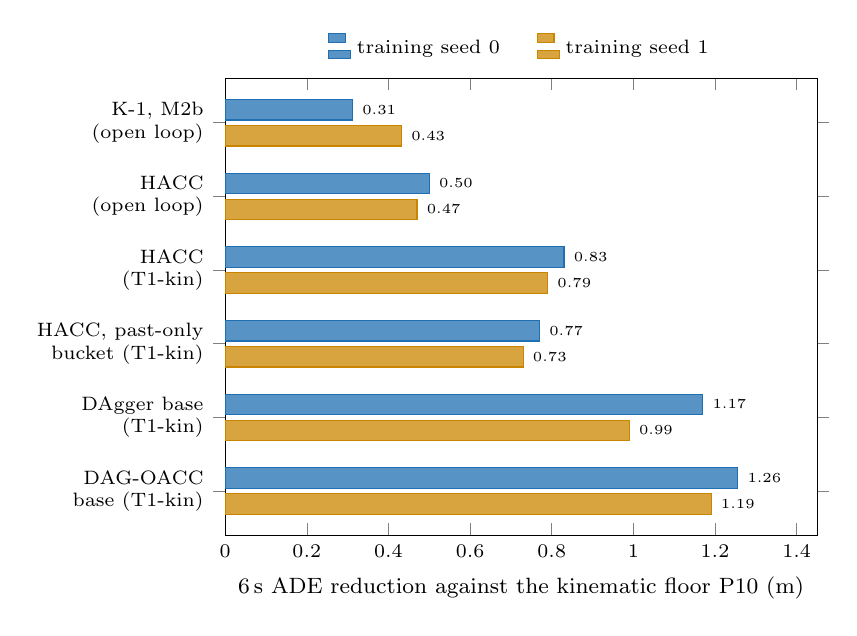
\begin{tikzpicture}
\begin{axis}[
  xbar, scale only axis, width=0.62\columnwidth, height=58mm, bar width=2.6mm,
  xmin=0, xmax=1.45, xlabel={6\,s ADE reduction against the kinematic floor P10 (m)},
  xlabel style={font=\footnotesize}, ticklabel style={font=\scriptsize},
  symbolic y coords={DAGO,DAG,HACCc,HACCt,HACCo,K1},
  ytick=data, yticklabel style={align=right},
  yticklabels={{K-1, M2b\\(open loop)},{HACC\\(open loop)},{HACC\\(T1-kin)},{HACC, past-only\\bucket (T1-kin)},{DAgger base\\(T1-kin)},{DAG-OACC\\base (T1-kin)}},
  enlarge y limits=0.12,
  legend style={font=\scriptsize,at={(0.5,1.02)},anchor=south,legend columns=2,draw=none,fill=none,/tikz/every even column/.append style={column sep=4mm}},
  nodes near coords, nodes near coords style={font=\tiny,anchor=west}, reverse legend,
  point meta=explicit symbolic,
]
\addplot[fill=levO!75,draw=levO] coordinates {(0.432,K1)[0.43] (0.47,HACCo)[0.47] (0.79,HACCt)[0.79] (0.73,HACCc)[0.73] (0.99,DAG)[0.99] (1.1903,DAGO)[1.19]};
\addplot[fill=levT!75,draw=levT] coordinates {(0.312,K1)[0.31] (0.50,HACCo)[0.50] (0.83,HACCt)[0.83] (0.77,HACCc)[0.77] (1.17,DAG)[1.17] (1.2556,DAGO)[1.26]};
\legend{training seed 1, training seed 0}
\end{axis}
\end{tikzpicture}
\caption{\textbf{Six-second error reduction against the learned kinematic floor}, at two training seeds. Every bar is a paired
episode-cluster bootstrap contrast on 141 held-out episodes, and every one is separated from zero. The tier is given per bar.}
\label{fig:bars}
\end{figure}

\begin{table}[!tp]
\centering
\caption{\textbf{Headline results} (MEASURED; paired episode-cluster bootstrap, $B=2000$, 141 episodes; values at seed 0 / seed 1).}
\label{tab:headline}
\small
\begin{tabularx}{\columnwidth}{@{}>{\raggedright\arraybackslash}Xl@{}}
\toprule
Result & Tier \\
\midrule
6\,s ADE $-0.312$\,/\,$-0.432$\,m vs P10, beyond the pre-registered $2F=0.2415$\,m (12.5--17.4\,\% lower error) & open loop \\
HACC post-map: better than P10 on \emph{every} row of the pre-registered set (ADE2, ADE6, accel., curvature, speed, heading, yaw rate, decisions, consistency) & open loop \\
6\,s ADE $-0.83$\,/\,$-0.79$\,m vs P10 on own executed motion; $-0.77$\,/\,$-0.73$\,m with a past-only speed bucket & T1-kin \\
Route checkpoints beat a kinematic arc by 1.2/3.3/7.8\,m and 1.3/3.5/8.8\,m at 30/50/80\,m & T1-kin \\
DAgger: tactical macro-F1 $+0.108$/$+0.118$ (lateral), $+0.055$/$+0.081$ (longitudinal); 6\,s ADE $-0.54$/$-0.40$\,m vs its control & T1-kin \\
Adopted base: 6\,s ADE $-1.26$\,/\,$-1.19$\,m vs P10; every family has a separated-better row & T1-kin \\
Per band: DAgger rows lower 2--6\,s ADE by 0.82\,/\,0.62\,m; the acceleration term lowers 0--2\,s ADE by 0.062\,/\,0.079\,m and 0--2\,s acceleration error by 0.97\,/\,1.14\,m/s$^2$ & T1-kin \\
Band loss, operative level detached: 0--2\,s ADE $-0.017$\,/\,$-0.015$\,m beyond a same-recipe replicate; no 2--6\,s row moves & T1-kin \\
Top-3 tactical manoeuvres contain the logged one in 90\,\% of windows (top-1: 57--59\,\%); best of three plans $-0.35$ to $-0.39$\,m 2--6\,s ADE (oracle) & T1-kin \\
Tactical headroom: 87\,/\,89\,\% in the continuous constraints; a forced correct stop lowers stop-point tactical ADE by 1.54\,/\,1.48\,m; stop re-weighting moves recall only along one ROC curve (oracle) & T1-kin \\
Ground-truth tactical code: 6\,s ADE from $\approx$2.1 to $\approx$1.0\,m (interface headroom) & T0 \\
Distance rule on the plan, lead from labels (privileged): unsafe rate 0.1275 to 0.0489 (hierarchy), 0.1296 to 0.0498 (grid state), six of six seeds; from the model's own vision head about 13 to 32 percent & T1-kin \\
Grid state, six paired seeds: 6\,s ADE $-0.0855$\,m $[-0.1705,+0.0044]$ (GRID-NO-COST); lead supervision: gap $R^2$ 0.544 to 0.737, closing speed flat (SUP-NO-COST) & T1-kin, T0 \\
Eighth of the clips against the full set: $+0.4311$\,m $[+0.1627,+0.6845]$ (DATA-SATURATED, KNEE-1/8); quarter $+0.1108$\,m $[-0.1505,+0.3822]$, open & T1-kin \\
Distance rule, vision-fed with a margin on the gap read calibrated on training clips: U 0.1246 to 0.0534 (LS) and 0.1343 to 0.0516 (LSD), reaches the label-fed rule (MARGIN-REACHES-ORACLE); price: 6\,s position error $+0.945$\,m and $+0.858$\,m (MARGIN-COSTS) & T1-kin \\
Rule in the training target: flat at 6,000 steps, $-0.0053$ $[-0.0281,+0.0119]$ (RULE-TRAINED-FLAT-6K); rule on the model's own plan: $-0.0276$ $[-0.0647,+0.0089]$ at $+2.67$\,m (OWN-RULE-FLAT, OWN-RULE-COSTS) & T1-kin \\
Imagined lead gap, response to the ego's acceleration: $-0.468$ $[-0.530,-0.415]$ (IMAG-DEAF; the logs give $-1.21$ $[-1.94,-0.30]$); consistency term at weight 0.0001 on rollout-loss bases: $+0.811$ $[+0.759,+0.866]$, imagination read kept (a dose arm, names nothing) & T0 \\
RR rollout, lead information beyond the present state on four seeds: $+0.025$ $[-0.000,+0.057]$ (MOTION-ADDS-NOTHING-4); forecast of future tokens, RR minus G: $+0.52$ $[+0.41,+0.63]$ (RR-FORECASTS-TOKENS-BETTER-4) & T0 \\
Planning by imagination, kinematic candidates: unsafe rate $-0.043$ $[-0.082,-0.013]$ against no tool, equal to extrapolation of the lead (IMAG-LEVEL-EQUALS-EXTRAPOLATION); response control not met, $+0.495$ and $+0.479$ against 0.5 & T1-kin \\
Trained gap head in the distance rule (LSD, all training clips): U against the calibrated map $-0.0098$ $[-0.0302,+0.0103]$, 6\,s error $-0.199$\,m $[-0.391,-0.017]$ (QHEAD-U-EQUAL-QF, QHEAD-CHEAPER-QF); a cost against no rule stays (QHEAD-COSTS) & T1-kin \\
Consistency weight 0.0001 on two new bases: response $+0.820$ $[+0.766,+0.878]$ against $-0.746$ $[-0.823,-0.676]$, level ratios 1.141 and 1.059 against the bar 1.15, no cost (LOW-WEIGHT-CONFIRMED); weight 0.001: $+0.971$ $[+0.907,+1.047]$, level ratios 1.710 and 1.252 (DOSE-BREAKS-AT-0.001) & T0, T1-kin \\
Level term, weights 0.001 and 0.01: response $+0.9034$ $[+0.8554,+0.9535]$ with level ratios 1.1060 and 1.1977, and $-0.4032$ $[-0.5492,-0.2681]$ with 1.0395 and 1.0525 (LEVEL-TERM-LOSES-LEVEL-0.001, LEVEL-TERM-LOSES-RESPONSE-0.01; row 92) & T0 \\
Planner on imagined rollouts at two new bases: U $-0.0347$ $[-0.0582,-0.0146]$ against off (IMAG-LEVEL-CUTS-UNSAFE-CONFIRMED); against extrapolation of the lead $+0.0169$ $[+0.0035,+0.0316]$ (IMAG-LEVEL-WORSE-THAN-EXTRAPOLATION) & T1-kin \\
Inference-side candidate (readout K, lead rule, second look) against the convention with the rule, label-fed: speed error $-0.635$\,m/s $[-0.743,-0.535]$, tactical ADE $-0.842$\,m $[-1.112,-0.627]$, route checkpoints $-3.48$/$-7.31$/$-12.32$\,m at 30/50/80\,m; U not separated, $-0.0018$ $[-0.0183,+0.0169]$ (row 121; unbounded executor) & T1-kin \\
\bottomrule
\end{tabularx}
\end{table}

\paragraph{The hierarchy beats its floor.} Against the learned kinematic floor P10, which is exactly the model's own output at a zero
residual by \cref{eq:traj}, v8F-mini (M2b) lowers 6\,s error by 0.312/0.432\,m at two seeds, beyond a pre-registered bar of twice the
seed floor (\cref{fig:bars}, \cref{tab:headline}). A zero-training post-map (HACC) blends O's plan with its own prior through
per-step weights fitted on training windows with an acceleration term. With it, the model is separated-better than P10 on every row of
a pre-registered set, including 2\,s error ($-0.011$/$-0.008$\,m), 6\,s error ($-0.50$/$-0.47$\,m) and acceleration
($-0.022$/$-0.040$\,m/s$^2$), and separated-worse on none.

\paragraph{The margin survives the model's own motion.} On T1-kin, where the ego state is rebuilt from the model's own executed motion at
each replan, the HACC model beats P10 by 0.83/0.79\,m. Two stress versions keep most of the margin:
\begin{itemize}
  \item a speed bucket rebuilt from the last 4\,s of measured speed alone keeps 0.77/0.73\,m;
  \item freezing the camera at the first frame for 6\,s as well keeps 0.73/0.64\,m.
\end{itemize}
The margin therefore rests on the model's reading of the scene and of its own state, not on future information.

\paragraph{On-policy data makes the tactical brain robust.} Replacing 10\,\% of training samples by the model's own rolled-out states
(DAgger, $p=0.1$) raises the tactical brain's lateral macro-F1 by 0.108/0.118 and its longitudinal macro-F1 by 0.055/0.081 on the
model's own motion. It also lowers executed 6\,s error by 0.54/0.40\,m. It is the first training lever to clear a T1 bar on both
heads. The adopted base built on it (DAG-OACC) lowers 6\,s error against P10 by 1.26/1.19\,m on its own motion. At least one row
improves in each of the four families (longitudinal, lateral, tactical and strategic).

\paragraph{Every level contributes.} The strategic brain's route checkpoints beat a kinematic arc at every horizon, by up to 8.8\,m at
80\,m. The tactical interface is used, as substituting the ground-truth code cuts 6\,s error from about 2.1 to about 1.0\,m.
\Cref{prop:lip} reads this as roughly 1.1\,m of headroom available through better tactical predictions. Because the response is
convex, that headroom concentrates in the final gains in tactical precision.

\paragraph{Which lever carries which band.} Under the band definition of \cref{sec:bands}, we retrained the operative and tactical levels with a per-band loss and with the operative level's loss detached from the tactical level, at two seeds and with a same-recipe replicate (\tier{T1-kin} throughout). The 0--2\,s plan improves at both seeds beyond the replicate: ADE by 0.017/0.015\,m, about 6\,\%, and FDE at 2\,s by 0.039/0.027\,m. No row of the 2--6\,s band moves, and the replicate says why: two runs of the same recipe differ there by 0.29\,m. A ladder of banked fine-tunes splits the adopted base into its three changes. The DAgger rows carry the tactical band (2--6\,s ADE $-0.82$/$-0.62$\,m, heading $-4.6$/$-2.6^{\circ}$). The acceleration-matching term carries the operative band and acceleration (0--2\,s ADE $-0.062$/$-0.079$\,m; acceleration error $-0.97$/$-1.14$\,m/s$^2$ at 0--2\,s and $-2.0$/$-2.6$\,m/s$^2$ at 2--6\,s). Decoding the operative level once per top-three tactical manoeuvre, the logged manoeuvre is among the three in 90\,\% of windows against 57--59\,\% for the first choice, and the best of the three plans would lower 2--6\,s ADE by 0.35--0.39\,m. That oracle gap is the measured headroom of a trained selection over the tactical codes, and the next lever.

\paragraph{Where the tactical headroom sits.} We measured that lever before building it, with zero-training oracle reads on the adopted recipe (\tier{T1-kin}, first tick, both seeds, every control at its known value; the strategic family paused). A perfect selector over the top three manoeuvres captures only 24/23\,\% of the best-of-three gain, so the choice among manoeuvres is not where the headroom lies. Writing the ground-truth tactical code in place of the model's own lowers tactical ADE by 1.63/1.77\,m. Leaving out its continuous constraints forfeits 87/89\,\% of that gain and leaving out the discrete decision 11/9\,\%; target speed is the costliest single constraint. The speed error spreads over every stratum, but stop-point windows hold 20\,\% of its squared mass on 5\,\% of the windows. There the decision misses: the goal head says stop in 10/13\,\% of the 117 stop-point windows, although its stop score separates them from the rest with AUROC 0.84/0.86. Forcing the correct stop into the tactical code lowers their tactical ADE by 1.54/1.48\,m (30--31\,\%), so the operative level executes a stop once it is decided.

Three pre-registered levers then acted on the decision alone. Hardening the model's own decision at inference recovers 3--6\,\% of that gain at a cost on the other windows, and a threshold chosen on training clips does not help. Re-weighting the stop classes at two doses raises stop recall from 0.06--0.15 to 0.45--0.62 and the false-stop rate from 0.5--1.3\,\% to 12--14.5\,\%, with AUROC unchanged within its replicate floor: the weights slide the operating point along one ROC curve and add no discrimination, and stop-point ADE does not improve beyond its 0.70\,m floor. The missing piece is discrimination, which is a perception question. Its ceiling was fixed before any training: a correct stop on the 82 of 117 stop-point windows that the model already ranks highest lowers tactical ADE there by 0.96/0.86\,m, beyond the floor at both seeds, with a separated lateral cost (yaw-rate error $+2.2^{\circ}$/s) that comes with the forced stop. Linear and small MLP probes on the frozen features rank stops no better than the model (AUROC 0.84--0.87 for every input set, a 4$\times$ finer token grid included), so the first perception arm trains instead of probing: a vision-only stop-location auxiliary loss, queued to train at two seeds against same-seed controls and two replicates. Two recipe levers closed on the way: on the DAgger base, detaching the operative level costs nothing, and the band loss's operative gain shrinks to 1--2\,mm and does not settle over four seeds.

% =====================================================================================================================
\subsection{Testing the premises of the theory}\label{sec:premises}
Each read below was pre-registered with its controls and both outcomes, and is a \tier{T0} or \tier{T1-kin} diagnostic on logged
frames; the strategic family is paused for the reads dated before the PI ruling of 2026-11-16 and not computed for the later ones (\cref{sec:fam7}). Reads that do not yet exist are named as such, and their numbers are not in this version.

\paragraph{Hierarchy against a flat control (T2).} A flat control at matched budget cuts the interface between the tactical and the
operative level. On all windows, with on-policy (DAgger) data in both arms, the comparison is \emph{not established}: 6\,s ADE,
hierarchy minus flat, is $-0.345$\,m $[-0.442,-0.251]$ at seed 0 and $-0.054$\,m $[-0.161,+0.055]$ at seed 1 (\tier{T1-kin}, one run
per arm per seed). Split by window class, with the mode thresholds fixed before the read (1,305 selection-critical and 1,094
common-case windows), the hierarchy is ahead on selection-critical windows by 0.48/0.16\,m, separated at both seeds; without
on-policy data it is ahead by 0.18/0.12\,m, separated at one seed. On common-case windows it is ahead by 0.18\,m at seed 0 and behind
by 0.07\,m at seed 1 with on-policy data, and behind by 0.32/0.49\,m without. The difference between the two classes is negative and
separated in all four cells ($-0.29$, $-0.23$, $-0.50$, $-0.61$\,m). This is the pattern that \cref{prop:dom} permits: a gain where
modes separate, and none promised elsewhere. It is not yet the mechanism: an exact decomposition does not place the margin in the
selection term, and both arms miss the logged 12-cell mode on 53 to 71\,\% of windows. A commit rule does not bank the gain either.
Letting the hierarchy drive only where its tactical output is confident beats both arms in no cell, because that confidence
separates the two window classes at AUROC 0.64 only; by the break-even condition of \cref{sec:theory}, a gate at that AUROC banks an
estimated 0.3 to 7.4\,\% of what a gate with the logged class would. The lever is the accuracy of the decision, not a gate on it.
With one run per arm all of this is necessary evidence and not sufficient. The deciding experiment is 24 arms at six seeds, hierarchy against flat under both training protocols,
with seeds as the unit. A window class
reads for the hierarchy only when all six seed differences agree in sign and the two-level interval (seeds, then episodes) excludes zero.

\paragraph{The six-seed replicate.} All 24 arms are trained and read (\tier{T1-kin}, 2,399 windows of 141 episodes, 7,214,495 parameters in
every arm, every control at its known value, the strategic family paused). Under the primary protocol, the own-state fine-tune, the
outcome is HIER-DOMINATES: 6\,s ADE, hierarchy minus flat, is $-0.092$\,m $[-0.168,-0.025]$ on all windows and $-0.195$\,m
$[-0.293,-0.098]$ on selection-critical windows, with all six seed differences negative in both cells (exact sign-flip $p=0.031$, the
smallest value six seeds allow); on common-case windows it is $+0.0305$\,m $[-0.0541,+0.1202]$, open. By family on all windows:
cross-track error $-0.165$\,m $[-0.219,-0.097]$ and heading error $-1.76^\circ$ $[-2.24,-1.28]$ read for the hierarchy; the
longitudinal, lateral and joint manoeuvre error rates are lower by $0.100$ $[0.063,0.135]$, $0.045$ $[0.027,0.061]$ and $0.104$
$[0.065,0.143]$; tactical-band ADE is $-0.144$\,m $[-0.255,-0.043]$; speed and along-track error are open ($-0.087$\,m/s
$[-0.197,+0.003]$ and $+0.024$\,m $[-0.049,+0.103]$). Under the secondary protocol, training from scratch without own-state data, the
outcome is NOT-ESTABLISHED: $-0.158$\,m $[-0.266,-0.034]$ on selection-critical windows with five of six seed differences negative,
$+0.3025$\,m $[+0.1437,+0.4550]$ on common-case windows, where the flat control is ahead, and $+0.052$\,m $[-0.061,+0.169]$ on all
windows; there the flat control is also ahead on speed error ($+0.298$\,m/s) and on the longitudinal manoeuvre error rate ($+0.097$),
and the hierarchy on cross-track error ($-0.184$\,m). The label-swap control reads open in 20 of 20 draws. The advantage of the
hierarchy is therefore established where the model has been trained on its own executed motion and is not established without it.
Limits: one corpus of 4,512 training clips, one evaluation set, a kinematic rollout on logged frames; the stop-goal
decision is not in this read (headway is read in \cref{sec:dist}), and the planner is deterministic, so inference variance is not sampled.

\paragraph{A yardstick for the world model (T1, T6).} The latent features are slow: their lag correlation is 0.975 at 0.2\,s and 0.883
at 2\,s. Against a forecast of no change, the learned predictor's skill is $+0.001$ at 0.2\,s, where a cross-fitted closed-form ridge
reads $+0.022$, and $-0.15$/$-0.17$ at 2\,s, where the ridge reads $+0.12$/$+0.13$ (\tier{T0}). A closed-form stack of the ridge and
the learned prediction reads $+0.040$, $+0.06$, $+0.15$ and $+0.17$ at 0.2, 0.4, 0.8 and 2.0\,s, above both parts at every horizon and
both seeds: weights written without a gradient step improve the world model. The premise of \cref{prop:jump} holds in the linear
class and strengthens with the horizon. The direct error is 0.74, 0.57, 0.52 and 0.42 of the composed one-step bound at 0.4, 0.8, 1.0
and 2.0\,s (0.416 $[0.389,0.449]$ at 2\,s). Multi-level prediction is therefore the right structure for these latents, and the learned
ten-step rollout is the part that fails. Even the stack explains only 4 to 17\,\% of the change, so the target space limits
imagination as well.

\paragraph{Rules by construction (T3).} Unshielded plans pass the logged rest point in 91.6/84.7\,\% of the 131 stop windows. The
verified shield, given the logged rest distance (a privileged ceiling), brings the overrun to exactly zero on every feasible window
and lowers stop-window 2--6\,s ADE by 3.51/3.37\,m with no cost in any cell (\tier{T1-kin}). Given the stop position that the model
itself emits (median error 11.8/9.6\,m, a flag on 10/18 of the 131 windows) it gains nothing. A split-conformal margin behaves as
proved, with held-out coverage 0.908 for a nominal 0.9, at the price of a margin of about 7.4\,m. Probes on the frozen tokens do not
supply the cue: ego kinematics alone rank stops at AUROC 0.810 $[0.744,0.868]$, and adding the $8\times20$ tokens changes that by
$-0.011$ $[-0.061,+0.043]$ (the stop label is derived from logged ego motion, so the ego baseline partly reads the source of its
own label). Rule adherence comes from the construction; usefulness comes from the sharpness of the cue.

\paragraph{The premise of the dominance theorem (T2), read.} For each context the selection premise asks whether the hierarchy
lands in the logged 12-cell mode more often than the largest logged cell holds (the margin, seed 0/1; \tier{T1-kin}, 2,399
windows, 141 episodes, zero training, controls pass). On all windows the margin is $+0.018$ $[-0.045,+0.079]$ and $-0.000$
$[-0.061,+0.059]$: undecided. At $v_0\in[8,15)$\,m/s (923 windows of 85 episodes) it is $+0.153$ $[+0.084,+0.229]$ and $+0.118$
$[+0.022,+0.215]$, so the premise holds at both seeds, and the flat arm has a margin of the same size there ($+0.118$/$+0.125$). Below
2\,m/s it fails at both seeds ($-0.171$ $[-0.326,-0.066]$ and $-0.242$ $[-0.401,-0.138]$), carried by the lateral mode (accuracy
0.218/0.237 against a largest class near 0.80, in both arms). The geometry premise fails in every context: the within-cell spread of
the logged 6\,s endpoints (13 to 81\,m) exceeds the distance between the two largest cells (separation index 0.149 $[0.047,0.232]$
pooled, at most 0.355 in a context), and among windows in the right mode the 90th percentile of the endpoint error is 8.7 to
15.4\,m against a tolerance of 2.0\,m. The 12 cells are therefore not modes in the sense of \cref{prop:dom}, and the theorem does
not imply dominance for v8F-mini in any context. Card outcomes with on-policy data in both arms: DOM-PREMISE-PARTIAL and
HIT-UNDECIDED; the hit rate at 2.0\,m, hierarchy minus flat, is $+0.032$ $[+0.011,+0.053]$ on selection-critical windows at seed 0
and $+0.012$ $[-0.007,+0.032]$ at seed 1. The committed next step is the same read on the six seeds of the replicate, with seeds as
the unit.

\paragraph{A located defect: at rest (HOLDREAD).} On the 211 windows that start below 2\,m/s (29 episodes) one fixed plan hits
31.3\,\% of the logged endpoints, the hierarchy 7.1/5.2\,\% and the flat arm 1.9/2.8\,\% (hit rate, hierarchy minus the best plan:
$-0.242$ $[-0.384,-0.103]$ and $-0.261$ $[-0.405,-0.132]$). In 53 of these windows the logged ego stays (14 episodes) and in 158 it goes.
Where it stays, the hierarchy travels a median of 8.68\,m $[6.87,10.48]$ and 11.83\,m $[8.53,14.45]$ and the flat arm 12.84/11.33\,m
(outcome CREEP). The plan at the window start separates go from stay at AUROC 0.803 $[0.711,0.894]$ and 0.807 $[0.706,0.907]$,
with lower bounds under the bar of 0.80 (CUE-WEAK). A hold rule keyed on that plan, emulated on banked rollouts and cross-fitted,
changes 6\,s ADE at rest by $-0.239$\,m $[-0.595,+0.073]$ and $-0.407$\,m $[-0.772,+0.016]$: both intervals include zero
(HOLD-UNDECIDED). With the logged stay label (a privileged ceiling) it would change it by $-0.542$ $[-0.855,-0.270]$ and $-0.515$
$[-0.826,-0.254]$. At rest the logged future has two modes and both arms drive a blend of them; a decided hold is worth about
0.5\,m when its cue is right, and the plan is not a sharp enough cue. The committed next step is a go-or-stay cue from perception,
which needs a probe or a training arm on training clips and was blocked on pod compute when the row was written.

\paragraph{A class weight is one number (T4).} Adding one scalar to the stop-goal bias of the unweighted model reproduces what a full
training run with a stop class weight does to the stop decision. At the offset that matches the trained false-positive rate, the hit rate
is within the replicate gap of the trained arm in all four cells (differences 0.009--0.026 against a gap of 0.068), and the stop
AUROC stays at 0.819/0.850 (\tier{T1-kin}, first tick). A dose is an edit that costs seconds; a better stop decision needs a better cue.

\paragraph{What the camera interface carries (T5).} The frozen tokens carry non-ego content beyond ego motion on four targets
(\tier{T0}, 139 episodes): lead gap $+0.29$ $R^2$ $[+0.11,+0.55]$, nearest agent $+0.15$, agent count $+0.16$ and lead presence $+0.18$
AUROC $[+0.09,+0.27]$. A prediction of ours failed here. From the camera geometry we had expected that no reader of the $4\times10$
tokens recovers far range; measured, they carry range beyond ego motion in the far stratum, and under a rank-256 probe an $8\times20$
grid adds nothing (lead gap $+0.011$ $R^2$ $[-0.023,+0.048]$). The probe rank hid part of the answer: with a full-kernel probe the
finer grid is ahead by $+0.076$ $R^2$ $[+0.001,+0.170]$ on lead gap and $+0.043$ AUROC $[+0.022,+0.066]$ on lead presence. Read
directly with an attentive probe, un-pooled $16\times40$ tokens give lead gap $R^2$ 0.46, against 0.40 for the $4\times10$ grid and 0.13
for ego motion alone; the best fine set gains $+0.055$ $[+0.000,+0.111]$, under its bar of 0.10, and lead presence rises from AUROC
0.77 to 0.84 ($+0.066$ $[+0.033,+0.103]$). The probes are still rising at 111 training episodes, so these reads are lower bounds.
A finer interface is a live but thin lever; the larger gap lies between what the tokens carry and what the model's own state exposes.

\paragraph{The world-model state, untrained and trained (T5, T7).} \Cref{prop:pool} was written before its controls. On real tokens a
planted object's position is read at AUROC 1.000 from a state that keeps the cell layout and 0.495 from the mean state, and a planted
motion at 1.000 from two frames of the grid state and 0.493 from two frames of the mean state. Without training, the lead gap is read
at $R^2$ 0.40 from the grid state, 0.26 from the mean state and 0.13 from ego motion alone; grid minus ego is $+0.27$ $[+0.08,+0.54]$,
and grid minus mean, $+0.14$ $[-0.004,+0.29]$, does not exclude zero on 139 episodes. On the \emph{trained} model the mean state was read at
two training seeds. Out of sample it tells whether a lead vehicle is present at AUROC 0.807/0.788, against 0.596 from ego motion
(differences $+0.211$ $[+0.105,+0.314]$ and $+0.192$ $[+0.101,+0.286]$). On 1,200 training clips it reads the lead gap at $R^2$ 0.456/0.445
against 0.187. For the \emph{change} of that gap over 2\,s, ego motion alone has a skill of $+0.291$ over persistence, and adding the
state adds nothing: $-0.028$ $[-0.065,+0.008]$ and $-0.025$ $[-0.059,+0.009]$. The two training runs differ by 0.010 in gap $R^2$ (a third baseline seed widens the range to 0.045). The
trained state knows where the lead is, and nothing about where it is going beyond ego motion: \cref{prop:pool} on a trained model.
Decoded back to pictures, the state shows the scene gist (sky, road, light level) and no object, at a skill of 0.36/0.35 against 0.78
for the token grid, and its learned 2\,s rollout is no closer to the true future frame than the present frame. By T7, imagination is
admissible for the gist and not for objects. The reads of a state that keeps the cell layout, and of a mean state of equal
width as its control, are in \cref{sec:state}.

\paragraph{Weight space (T9).} The 50/50 weight average of two same-initialisation replicates lowers tactical ADE by 0.075\,m
$[0.047,0.103]$ against the member mean and realises $\kappa=0.74$ $[0.48,0.99]$ of the gain of an output ensemble, in one forward pass
and with no separated cost in any family (\tier{T1-kin}). It is not ahead of the better member; what it removes is the risk of the
worse one. Read in weight space (one replicate pair, no interval), a stop class weight moves the model less than a change of seed does in every module group, and
clearly exceeds seed noise only in two head biases, which is what T4 says a class weight is.

\paragraph{Data (T8).} At the probe level, choosing 25 or 50\,\% of the training episodes by coverage or by leverage in token space
lands inside the range of 20 random draws, so no selection claim is made for this representation. The trained arms are in
\cref{sec:dataeff}.

\subsection{A world-model state that keeps the layout}\label{sec:state}
\Cref{prop:pool} says what a mean over cells cannot hold; the least change is to keep the cells. Arm G keeps the layout (40 cells of
16 numbers, 9,091,503 trainable parameters), arm W is a mean state of equal width (640, 9,251,871 parameters) and the baseline is
the mean state of 128 numbers (7,214,495 parameters); each trained 19,164 steps, G and W at two seeds, the baseline at three. All
reads below are \tier{T0} world-model diagnostics on logged frames, with every control passing first.

\paragraph{The gain is the layout, not the width.} Out of sample (139 episodes, lead gap on 2,485 frames), the lead gap is read at
$R^2$ 0.552 $[0.419,0.651]$ and 0.541 $[0.414,0.633]$ from G, 0.361 $[0.146,0.518]$ and 0.309 $[0.115,0.455]$ from W, 0.237, 0.212
and 0.143 from the three baseline seeds, and 0.133 from ego motion; the state minus ego motion is $+0.419$ $[+0.212,+0.708]$ and
$+0.409$ $[+0.192,+0.710]$ for G (values of different arms are side by side, not paired). On 1,200 training clips, paired over
clips, G minus W is $+0.104$ $[+0.074,+0.134]$ and $+0.116$ $[+0.087,+0.146]$, and W minus the baseline is $-0.008$ $[-0.027,+0.010]$
and $+0.009$ $[-0.010,+0.029]$, against a baseline range of 0.045 over three seeds: the gain is assigned to \emph{location} in the
sense of the card. Lead presence reads at AUROC 0.860 $[0.802,0.906]$ and 0.862 $[0.807,0.908]$ for G, 0.819 and 0.789 for W,
0.807/0.788/0.792 for the baseline and 0.596 for ego motion. Decoded to pictures, the held-out skill is 0.605 $[0.567,0.641]$ and
0.555 $[0.510,0.597]$ for G against 0.777 $[0.752,0.801]$ for the token grid (ratio 0.78/0.72, the bar for the strongest name is
0.90, so the outcome is Z-ABOVE-MEAN), $+0.244$ $[+0.210,+0.276]$ and $+0.202$ $[+0.167,+0.237]$ above the baseline of the same
seed, while W reads 0.338 $[0.272,0.405]$ and 0.345 $[0.283,0.410]$ (Z-FLAT at both seeds); G minus W is $+0.267$ $[+0.229,+0.304]$
and $+0.210$ $[+0.173,+0.246]$. What the layout does not give is the \emph{change}: over 2\,s, the state with history minus the
ego block is $-0.050$ $[-0.094,-0.004]$ and $-0.057$ $[-0.104,-0.009]$ for G and $-0.032$ $[-0.070,+0.008]$ and $-0.017$ $[-0.053,+0.019]$
for W; no state adds to ego motion. The four-family read finds no cell worse (\cref{tab:fam6}).

\paragraph{Why the rollout was flat.} Rolled out 2.0\,s by the predictor of its own arm, the grid state does not read the lead
better than a copy of the present state: rolled-out, present and true future state read 0.442, 0.496 and 0.552 for G at seed 0
(rollout minus copy $-0.054$ $[-0.154,+0.033]$ and $-0.036$ $[-0.153,+0.064]$ at seeds 0 and 1; W $-0.079$ $[-0.226,+0.052]$ and
$-0.093$ $[-0.326,+0.119]$), the outcome IMAGINE-FLAT, and the same name in pixels (rollout minus copy at 2.0\,s $-0.00006$
$[-0.0005,+0.0004]$ and $+0.00065$ $[-0.0001,+0.0014]$ for G). Two reads without any training locate the cause. Seeding the
rollout with the true history changes nothing (the rule of the card names it CTX-FLAT: rollout minus copy $-0.034$ and $-0.004$,
and against the one-state rollout $+0.010$ $[-0.005,+0.030]$ and $+0.028$ $[+0.008,+0.055]$). And one step (0.2\,s) ahead the
error of the flat predictor is 1.233 $[1.180,1.295]$ and 1.254 $[1.197,1.317]$ times the error of copying the state on held-out
windows (W at seed 0: 1.026 $[1.013,1.042]$): it has not learned the change at the step it is trained on.

\paragraph{A predictor that attends across the cells.} The cell predictor has 873,488 parameters against 2,074,496 for the flat
one. One step ahead its error is 0.788 $[0.770,0.807]$ and 0.796 $[0.779,0.814]$ of the copy's. On the lead read at $+2.0$\,s (441
windows with a lead at both times), rolled-out, present and true future state read 0.501/0.487/0.532 at seed 0 and
0.506/0.483/0.551 at seed 1; rollout minus copy is $+0.013$ $[-0.037,+0.057]$ and $+0.023$ $[-0.032,+0.081]$, rollout minus the
ego floor $+0.322$ $[+0.116,+0.614]$ and $+0.327$ $[+0.101,+0.655]$, and the rollout of this predictor minus that of the flat one
$+0.058$ $[-0.030,+0.163]$ and $+0.069$ $[-0.017,+0.174]$. No interval of the two deciding lines excludes zero at either seed, so
the outcome is CELL-FLAT as written, with the wanted sign on every line. The position is kept: on the training clips the lead
gap $R^2$ differs from G by $+0.010$ $[-0.011,+0.031]$ and $-0.033$ $[-0.053,-0.014]$, the second below the baseline range of
0.045 (KEEPS-POSITION), and from the baseline by $+0.107$ and $+0.092$. In pixels the learned rollout is below the copy at 0.8\,s
($-0.00058$ and $-0.00072$) and flat at 2.0\,s ($+0.00044$ $[-0.0003,+0.0012]$ and $-0.00004$ $[-0.0005,+0.0004]$). The change
of the gap over 2\,s is the missing part: the true future state holds skill $+0.190$ and $+0.205$ over persistence, the rollout
$+0.007$ $[-0.103,+0.122]$ and $+0.056$ $[-0.037,+0.162]$. The family read with all six baseline seeds names NO-COST for the cell predictor against the grid state and against the baseline (joint mode error rate against the baseline $+0.0663$ $[+0.0346,+0.1007]$, inside the spread).

\paragraph{The two levers at both seeds, and the arms that exist.} Two levers were pre-registered before any of their numbers (cards ADD18 and ADD19). MOTION trains the predictor on its own 2.0\,s rollouts (arm PR on the cell predictor), has it output the state plus a change (RES), or both (RR). TARGET gives the predictor the measured ego speed as a third action channel (arm PE; by a note frozen before the gate its inverse-dynamics head is also trained to read the speed) or trains a linear head per cell on the frozen token grid of the future frame (arm PF). PR and PE now have both seeds, read against the cell predictor P (\cref{tab:levers}; step, lead, change and position reads are \tier{T0} diagnostics on logged frames, 441 windows with a lead at both times; the family read is \tier{T1-kin}; controls first). The names at both seeds: PR reads STEP-BELOW-COPY, MOTION-FLAT, MOTION-STILL, KEEPS-POSITION and NO-COST; PE reads STEP-SAME, TARGET-FLAT, TARGET-STILL, KEEPS-POSITION and NO-COST. The one-step error ratio over the copy is 0.844 $[0.831,0.857]$ and 0.873 $[0.864,0.883]$ for PR, above that of P by $+0.056$ and $+0.077$; the change skill of PR is against a ceiling of $+0.159$ and $+0.190$. Stated plainly beside NO-COST: PR has higher lateral errors than HIER at both seeds (heading $+1.273$\,deg, curvature $+0.0473$\,1/m, yaw rate $+3.68$\,deg/s), each inside the six-seed spread. RES, RR and PF have one seed and name nothing; RR at seed 0 alone reads MOTION-IMAGINES (rollout minus the ego floor $+0.306$ $[+0.087,+0.619]$), and it cannot be attributed to RES or to the rollout loss, since RES at seed 0 is flat and the ROLL arms are not trained. Control x1 is not evaluated for the new arms (the pixel job was not run), and the per-arm gate tokens were not re-checked in the collation. As the cards commit, PR leads to an explicit target of object motion (the PF lever, one seed so far) and PE to the object-level slot, since the hypothesis that the speed channel helps is not supported.

\begin{table*}[!tp]
\centering
\caption{\textbf{The two levers against the cell predictor P} (\tier{T0}; seeds 0 and 1 where both exist; PE position is without interval in the source). Rollout minus the copy, rollout minus the rollout of P, change skill of the rollout over persistence, and the position read as the arm minus G (PR) or as banked (others). A dash is a cell the source does not give. RES, RR and PF have one seed and name nothing.}
\label{tab:levers}
\scriptsize
\begin{tabularx}{\textwidth}{@{}l>{\raggedright\arraybackslash}X>{\raggedright\arraybackslash}X>{\raggedright\arraybackslash}X>{\raggedright\arraybackslash}X@{}}
\toprule
Arm, seed & Rollout minus copy & Rollout minus rollout of P & Change skill & Position \\
\midrule
PR, 0 & $+0.002$ $[-0.062,+0.065]$ & $-0.059$ $[-0.134,+0.013]$ & $+0.014$ $[-0.092,+0.130]$ & $-0.0005$ $[-0.019,+0.018]$ \\
PR, 1 & $+0.025$ $[-0.038,+0.084]$ & $+0.032$ $[-0.043,+0.105]$ & $+0.091$ $[-0.015,+0.212]$ & $-0.024$ $[-0.043,-0.005]$, below the spread 0.0450 \\
PE, 0 & $+0.021$ $[-0.028,+0.073]$ & $+0.021$ $[-0.041,+0.080]$ & $-0.064$ $[-0.179,+0.039]$ & $+0.007$ \\
PE, 1 & $+0.017$ $[-0.044,+0.079]$ & $-0.011$ $[-0.100,+0.065]$ & $+0.042$ $[-0.059,+0.142]$ & $+0.009$ \\
RES, 0 & $+0.017$ $[-0.021,+0.052]$ & -- & $+0.029$ & $-0.021$ $[-0.038,-0.004]$ \\
RR, 0 & $+0.050$ $[+0.003,+0.098]$ & -- & $+0.091$ $[-0.008,+0.212]$ & $+0.029$ $[+0.012,+0.047]$ \\
PF, 0 & $-0.082$ $[-0.206,+0.018]$ & -- & $-0.009$ & -- \\
\bottomrule
\end{tabularx}
\end{table*}

\paragraph{The grid state costs nothing on six paired seeds (SPATIALREP).} Four more seeds of the grid arm (G2 to G5) were trained on the pod under a gate PASS, 19,164 steps each, so that the grid state is read against the baseline with six paired seeds (\tier{T1-kin}, 141 episodes, 2,399 windows, two-level bootstrap over seeds and then episodes, $B=2000$; the reader controls all pass). G minus HIER on the 6\,s ADE of all windows (the primary cell) reads mean $-0.0855$\,m $[-0.1705,+0.0044]$ against a six-seed spread of the baseline of 0.2845\,m (\cref{tab:perseed}). Four of six differences are negative and the interval includes 0: GRID-NO-COST. No cell of the four families is worse (STRATEGIC: PAUSED, PI item 25). The first two seeds alone read $-0.1198$\,m $[-0.1982,-0.0349]$; four more seeds brought two positive differences, so that read was inside the run-to-run variation of training. Common-case windows $-0.1522$\,m $[-0.2623,-0.0312]$, speed error and cross-track error (\cref{tab:fam6}) are five of six negative and inside the spread, and name nothing. The final read of the state arms at six baseline seeds and two seeds per arm (card ADD12, \tier{T1-kin}) agrees: grid, wide mean state and cell predictor against the baseline, grid against the wide mean state and cell predictor against the grid all name NO-COST (cross-track of the grid $-0.1071$\,m, inside the spread). The committed step: the grid state stays the state of the world-model path (it holds the lead position, at one-frame probe $R^2$ 0.552/0.541) and is the base of the lead-supervision arms of \cref{sec:lead}.

\begin{table*}[!tp]
\centering
\caption{\textbf{Per-seed differences of the six-seed reads} (\tier{T1-kin}; seeds 0 to 5; the mean carries the two-level interval; spread = largest difference between baseline seeds). The first row is in metres of 6\,s ADE on all windows; the others are the unsafe rate U (share of lead windows with an unsafe step of the model among the windows where the driver has none).}
\label{tab:perseed}
\scriptsize
\begin{tabularx}{\textwidth}{@{}>{\raggedright\arraybackslash}p{36mm}cccccc>{\raggedright\arraybackslash}X@{}}
\toprule
Difference & s0 & s1 & s2 & s3 & s4 & s5 & Mean $[$interval$]$, name \\
\midrule
G minus HIER, ADE 6\,s (spread 0.2845) & $-0.1011$ & $-0.1384$ & $+0.0421$ & $-0.1174$ & $+0.0298$ & $-0.2281$ & $-0.0855$ $[-0.1705,+0.0044]$, GRID-NO-COST \\
HIER minus FLAT, U (spread 0.0463) & $-0.0267$ & $+0.0160$ & $+0.0214$ & $-0.0214$ & $-0.0320$ & $+0.0089$ & $-0.0056$ $[-0.0269,+0.0140]$, DISTANCE-EQUAL \\
Rule minus no rule, HIER, label-fed, U & $-0.0623$ & $-0.0890$ & $-0.1050$ & $-0.0747$ & $-0.0641$ & $-0.0765$ & $-0.0786$ $[-0.1015,-0.0557]$, RULE-CUTS-UNSAFE \\
Rule minus no rule, G, label-fed, U & $-0.0765$ & $-0.0730$ & $-0.0996$ & $-0.0658$ & $-0.0747$ & $-0.0890$ & $-0.0798$ $[-0.1024,-0.0596]$, RULE-CUTS-UNSAFE \\
\bottomrule
\end{tabularx}
\end{table*}

\subsection{What the state holds of the lead's motion}\label{sec:lead}
The open problem of \cref{sec:state} is the lead gap 2.0\,s ahead. Every read below is a \tier{T0} diagnostic on logged frames, scored on 429 windows of 48 evaluation episodes (413 with a closing-speed label), episode-cluster bootstrap ($B=2000$), every control at its known value first. The three families other than STRATEGIC (PAUSED, PI item 25) are not measured by these reads.

\paragraph{A kinematic slot reads the gap when its inputs are right (OBJSLOT).} Two numbers per lead vehicle (gap, closing speed) and one kinematic identity, with zero training, on 1,948 windows of 139 episodes (lead at the start and at the target in 471, 42 dropped by the continuity rule). With the logged gap as input (a privileged ceiling), constant lead speed with the known ego motion (rule R2) reads skill $+0.750$ $[+0.664,+0.811]$ over the copy and constant closing speed (R1) $+0.692$ $[+0.588,+0.766]$; the level $R^2$ is 0.952 against 0.810 for the copy and the RMSE 2.18 against 4.36\,m: KIN-CEILING-HOLDS (the lead recomputed the label numbers with independent rule code: 0.7499, 0.6916, 0.9524, 0.8097). With the gap read from the grid state (vision only), R1 and R2 are below the copy in every arm (R2 skill $-0.236$, $-0.329$, $-0.407$, $-0.304$ for P and G at seeds 0 and 1) and the rule with a cross-fitted residual (R3, primary) reads $+0.011$, $+0.003$, $-0.007$ and $+0.027$, every interval including 0: SLOT-FLAT for the cell-predictor and the grid-state arms. The transition is therefore not the missing part, since the fixed rule halves the error once its two inputs are right; the missing part is a read of the gap and of the closing speed at the needed precision (the level $R^2$ of the vision copy is 0.54 to 0.56 against 0.81 for the label copy).

\paragraph{A head on five frames of the state, and the same head on 17 times more rows (LEADHEAD).} Stage 0 fits a head supervised on gap and closing speed over the five-frame history of the grid state, cross-fitted by episode on the evaluation bank: 6,997 to 7,064 fit rows per fold, of which 1,689 to 1,926 carry a closing-speed label, for 3,200 inputs (26 of 26 controls pass). The held-out closing-speed $R^2$ of the temporal ridge is negative in every arm (\cref{tab:leadA}), RMSE about 2.4\,m/s, and the small network is lower ($-0.275$ to $-0.288$): HEAD-CLOSING-FLAT; the slot read (R3 over the head copy $-0.045$, $-0.018$, $-0.002$, $+0.083$, every interval including 0) is HEAD-SLOT-FLAT; the direct supervised read of the change over 2.0\,s is below its copy in every arm: STATE-LACKS-FUTURE. The card names the limit beside them: too few rows for the input width. Stage 0b fits the same heads on 1,200 training clips disjoint from the evaluation episodes (32,025 gap, 30,865 closing-speed and 24,533 direct rows; controls j1 to j8 pass). One of four closing-speed intervals excludes 0, so by the rule of the card the names are HEAD-CLOSING-FLAT-B and HEAD-SLOT-FLAT-B (slot $+0.095$, $+0.099$, $+0.100$, $+0.104$, every interval including 0) for both arm types; the direct read of the change over 2.0\,s is above its head copy in all four arms with lower ends above 0 (+0.023, +0.043, +0.029, +0.018): STATE-HOLDS-FUTURE-B. The learning curve rises at every step and has not flattened (no exponent is fitted or quoted), so, as the card commits for a rising curve, these names are not read as a property of the state until the fit set is extended; the extension is the LEADSUP arms below.

\begin{table*}[!tp]
\centering
\caption{\textbf{Lead heads on the state of P and G, two reads} (\tier{T0}; P and G at seeds 0 and 1; $R^2$ unless marked). Stage 0 has 1,689 to 1,926 closing-speed rows, stage 0b all rows of the train probe set; intervals are given where the source gives them.}
\label{tab:leadA}
\scriptsize
\begin{tabularx}{\textwidth}{@{}>{\raggedright\arraybackslash}p{50mm}>{\raggedright\arraybackslash}X>{\raggedright\arraybackslash}X>{\raggedright\arraybackslash}X>{\raggedright\arraybackslash}X@{}}
\toprule
Read & P, 0 & P, 1 & G, 0 & G, 1 \\
\midrule
Stage 0, closing speed, ridge & $-0.094$ $[-0.238,+0.012]$ & $-0.108$ & $-0.098$ & $-0.060$ \\
Stage 0b, closing speed, ridge, all rows & $+0.126$ $[-0.048,+0.227]$ & $+0.145$ $[-0.020,+0.245]$ & $+0.101$ $[-0.083,+0.206]$ & $+0.176$ $[+0.012,+0.278]$ \\
Stage 0b, direct change skill over the head copy & $+0.100$ $[+0.023,+0.170]$ & $+0.119$ & $+0.115$ & $+0.090$ \\
Learning curve, closing speed, 2,000 rows & $-0.155$ & $-0.046$ & $-0.132$ & $-0.155$ \\
\hspace{3mm}8,000 rows & $+0.011$ & $+0.031$ & $+0.023$ & $+0.041$ \\
\hspace{3mm}16,000 rows & $+0.062$ & $+0.060$ & $+0.048$ & $+0.101$ \\
\hspace{3mm}all rows & $+0.126$ & $+0.145$ & $+0.101$ & $+0.176$ \\
\bottomrule
\end{tabularx}
\end{table*}

\paragraph{Asking during training (LEADSUP, card ADD24).} The term is a supervised lead head on the level-1 grid state with a label rule on gap, closing speed and presence. The build is checked and gated before any arm trained: with the flag off the patched trainer equals the base bit for bit on three argument sets; the new term alone reaches the head (gradient 64.1) and the adapter (30.1) and reads exactly 0.0 on the level-1 predictor and the driving heads, while the total reaches those (control); three mutations go red; the arm adds 82,499 parameters. Three arm types, two seeds each, 19,164 steps under a gate PASS: LS (weight 1), LSH (weight 10) and LSD (weight 1, head on the detached state). \emph{By the card as written no outcome is named:} control k5 (the mean of the lead term over the last 1,000 steps below its mean over the first 1,000) FAILS for all six arms (LS 0.3027 to 0.3741 and 0.2867 to 0.3540; LSD 0.3798 to 0.4337 and 0.3710 to 0.4066; LSH 0.2119 to 0.3190 and 0.2088 to 0.2897), and the card says an arm that fails k5 is not read. The slot part of control k3 in the card form passes for LS ($+0.019$, $+0.016$) and fails for LSH ($+0.095$, $+0.028$) and LSD ($+0.055$, $+0.062$) against the bar $+0.02$. Measured on the logs: the lead term falls within the first 300 steps, its presence part then rises and stays higher, the gap part falls over the run in every arm, and the closing-speed part in none. \emph{Read under notes N1 and N2} (N1 defines an attributable slot increment, frozen before seed 1 existed; N2 replaces k5 by k5-N2, frozen after the logs and the seed-0 reads were seen and before any lead-read number of a seed-1 arm; its log parts were written after the logs and add little, the held-out part carries it; k5-N2 passes for all six arms): the closing-speed $R^2$ has every interval including 0, SUP-CLOSING-FLAT in all three arm types (\cref{tab:leadB}); the gap $R^2$ of the head is 0.544 to 0.737 (RMSE 5.3 to 6.9\,m) and the presence AUROC 0.904 to 0.922; the slot increment DELTA reads SUP-SLOT-FLAT-N1 in all three; the gradient question, paired, reads SUP-GRADIENT-EQUAL twice (LS minus LSD $-0.024$ $[-0.164,+0.132]$ and $-0.075$ $[-0.328,+0.156]$; floor 0.089). The cost read (\tier{T1-kin}, 2,399 windows of 141 episodes, spread of G on six seeds 0.4002 on the primary cell) names SUP-NO-COST for all three: no cell worse under the rule in the longitudinal, lateral or tactical family; the primary cell is $-0.1150$\,m $[-0.1995,-0.0274]$ for LS minus G (inside the spread, not an effect), $-0.0179$ $[-0.1239,+0.0909]$ for LSH and $+0.0746$ $[-0.0707,+0.2154]$ for LSD; LS minus LSD has one cell better (joint class error $-0.0604$ $[-0.0953,-0.0248]$, spread 0.0492). Asking for the lead during training therefore gives a gap read and a presence read at no cost in the rollout, and no closing speed. A limit of that reading was measured after the card was frozen (control p2b of card ADD27, synthetic): a head of this form trained by gradient steps does not take a rate from five frames of a planted gap, so the head is a second candidate for the limit beside the cue.

\begin{table*}[!tp]
\centering
\caption{\textbf{LEADSUP and GAPFILTER, six arms} (\tier{T0}; 413 scored windows; read under notes N1 and N2 for LEADSUP, card form of GAPFILTER; seed 0 / seed 1 inside each cell). The filter rows are the numbers of the GAPFILTER card run, whose control f2 fails as written (no outcome named).}
\label{tab:leadB}
\scriptsize
\begin{tabularx}{\textwidth}{@{}>{\raggedright\arraybackslash}p{34mm}>{\raggedright\arraybackslash}X>{\raggedright\arraybackslash}X>{\raggedright\arraybackslash}X@{}}
\toprule
Quantity & LS & LSH & LSD \\
\midrule
Closing speed $R^2$ of the head & $+0.155$ $[-0.043,+0.283]$ / $+0.014$ $[-0.278,+0.192]$ & $+0.092$ $[-0.138,+0.231]$ / $+0.026$ $[-0.192,+0.163]$ & $+0.178$ $[-0.059,+0.335]$ / $+0.089$ $[-0.127,+0.234]$ \\
Gap $R^2$ of the head & 0.724 / 0.580 & 0.595 / 0.737 & 0.626 / 0.544 \\
Slot increment DELTA (note N1) & $-0.004$ $[-0.026,+0.016]$ / $-0.004$ $[-0.059,+0.051]$ & $+0.019$ $[-0.027,+0.067]$ / $+0.001$ $[-0.085,+0.060]$ & $+0.001$ $[-0.044,+0.045]$ / $-0.032$ $[-0.066,+0.004]$ \\
Closing speed $R^2$ of the alpha-beta filter & $+0.130$ $[-0.058,+0.256]$ / $+0.177$ $[-0.019,+0.290]$ & $+0.201$ $[-0.005,+0.322]$ / $+0.158$ $[-0.064,+0.282]$ & $+0.149$ $[+0.008,+0.229]$ / $+0.102$ $[-0.062,+0.206]$ \\
Filter minus the head's own output & $-0.025$ $[-0.163,+0.113]$ / $+0.164$ $[-0.035,+0.419]$ & $+0.110$ $[-0.090,+0.312]$ / $+0.132$ $[-0.079,+0.317]$ & $-0.029$ $[-0.178,+0.145]$ / $+0.013$ $[-0.141,+0.185]$ \\
\bottomrule
\end{tabularx}
\end{table*}

\paragraph{Taking the rate outside the network, and a probe of the tokens (GAPFILTER, TOKPROBE).} Card ADD28 asks whether a causal filter over the head's own per-frame gap reads the closing speed on a longer baseline, with zero training. \emph{By the card as written control f2 fails and the card names no outcome:} the slope estimator on the label gap must read the label closing speed at $R^2$ of at least 0.8 and reads $+0.367$; 410 of 413 windows reproduce the label exactly, and the 3 windows with a change of lead inside the last five frames are the ones where the estimator as the card words it fits across the step. Controls f1, f3, f4, f5 and f6 pass for all six arms. The numbers of the card run are in \cref{tab:leadB}: every arm selects the alpha-beta filter (alpha 0.7; beta 0.1, for LSD at seed 1 0.05), every interval of the filter's gain over the head includes 0, and so does every slot increment with the filter rate ($-0.003$ to $+0.029$); no arm type would have met the rule of FILTER-READS-CLOSING had f2 passed. A variant with a same-lead rule (a step above 3.0\,m restarts the run), written after f2 was seen and naming nothing, passes all its controls (f2 $R^2$ $+1.000$) and is flat too (filter $R^2$ $+0.09$ to $+0.24$). Why it is flat, measured (report f7): the head's gap error on evaluation rows is 7.0 to 8.8\,m RMSE and its change between consecutive rows (0.2\,s) 2.2 to 2.3\,m RMSE, with lag-1 autocorrelation 0.95 to 0.96, a slow drift a filter cannot remove; a rate needs a read about 0.5\,m coarse from frame to frame (report f8: closing-speed $R^2$ $+0.90$ at 0.5\,m of white noise on the label gap, $+0.43$ at 1\,m, below 0 at 2\,m). The token probe (card ADD27) has its instrument checked first: its gap-only control p2b, in the wording of the card, FAILS on synthetic data (held-out gap $R^2$ 0.90 to 0.95, closing-speed $R^2$ at most $+0.091$ where a slope on the known directions reads $+0.936$). Note ADD27\_N1, frozen before this result, fixes the consequence: the card can name TOKENS-HOLD-CLOSING and cannot name TOKENS-FLAT. The probe arms have since been run on real tokens; the read follows this paragraph. A finer grid or a crop of the lead region at full resolution would need the camera frames re-encoded, a data and compute step the PI decides. Limits: two seeds per arm type, one corpus, and p2b is a small synthetic world.

\paragraph{The token probe on real tokens (TOKPROBE, card ADD27 with note N1).} The question was whether the 640-wide grid state is what stops the lead head from reading the closing speed, or whether the pooled camera tokens (40 tokens of 1,024 per frame, five frames) do not give it either. A per-token network and the lead head of card ADD24 were trained on the frozen tokens (widths 16 and 64, seeds 0 and 1) with the loss, batch, 19,164 steps and schedule of the lead-supervision arms, and read on 413 scored windows of 48 evaluation episodes (\tier{T0}, episode bootstrap, $B=2000$). Controls first: p1, p2a, p3, p5 and the reader controls pass; \emph{p2b fails} (with only the gap planted over the frames the probe does not derive the rate, closing-speed $R^2$ at most $+0.091$ where the oracle input reads $+0.936$), so by note N1 TOKENS-FLAT cannot be named. Closing speed $R^2$: probe width 16 $-0.002$ $[-0.398,+0.212]$ and $+0.203$ $[-0.023,+0.328]$, width 64 $+0.042$ and $-0.001$, the head on the grid state $+0.178$ and $+0.089$; paired against the head of the same seed no interval excludes 0 (width 16 $-0.1798$ $[-0.446,+0.024]$ and $+0.1143$ $[-0.086,+0.315]$; width 64 $-0.1359$ $[-0.360,+0.058]$ and $-0.0902$ $[-0.467,+0.174]$; floor from the two head runs 0.0893). No outcome is named: TOKENS-HOLD-CLOSING needs a read above the bar in both seeds, and TOKENS-FLAT is blocked by p2b. Beside, naming nothing: gap $R^2$ $+0.493/+0.704$ (width 16), $+0.563/+0.571$ (width 64) against $+0.626/+0.544$ for the head on the grid state, presence AUROC 0.866 to 0.900 against 0.904/0.909. For presence and gap the tokens give no better read than the grid state, so the 640-wide state is not what limits them; for the closing speed nothing can be said in either direction, because the instrument did not show that it can derive a rate. The gap read from the tokens drifts between frames as much as the one from the grid state (change between consecutive frames 2.32 to 2.46\,m, lag-1 autocorrelation 0.94 to 0.96, against 2.2 to 2.3\,m and 0.95 to 0.96 for the heads; a rate needs about 0.5\,m); the gap filter of card ADD28 on these arms keeps its control f2 failed as written and names nothing. A sensitivity pass in the literal form of the card (tokens not normalised; names nothing) reads the same picture. Limits: two seeds per width; a probe says what the pooled tokens allow, not what the model does; one corpus. The branch that would give a finer gap (unpooled tokens or a second encoder pass over the lead region) needs camera frames on the pod and stays a decision of the PI; the stored 8 by 20 grid is read without frames in a pilot pre-registered as card ADD41 (\cref{sec:status}).

\subsection{Distance keeping, and a rule on the plan}\label{sec:dist}
\paragraph{Distance keeping is now measured (HEADWAY).} Every \tier{T1-kin} read before this one reported the longitudinal family without headway and time gap. Read from the banked dumps and the lead labels of the evaluation episodes (no new rollout; 642 of the 2,399 windows have a lead, in 56 of 141 episodes): the lead keeps its logged track, the model gap is the logged gap plus the logged progress minus the rolled progress, and an unsafe step is a gap below 2.0\,m or a time gap below 1.0\,s. U is the share of lead windows with an unsafe step of the model among the windows where the driver has none. Controls h1 to h6 pass, each with its regression form failing as required (a planted advance of 0.5\,m/s read back as $-1.0$\,m at 2.0\,s and $-3.0$\,m at 6.0\,s and named worse; a 5-frame shift of the label mapping fails on 470 windows); an independent recomputation of U for HIER at seed 0 agrees (0.106761565836, difference 0.0). Over six seeds (two-level bootstrap, rule of card ADD11): HIER minus FLAT is $-0.0056$ $[-0.0269,+0.0140]$ against a spread of 0.0463 (\cref{tab:perseed}), DISTANCE-EQUAL, and G minus HIER is $+0.0021$ $[-0.0136,+0.0175]$, GRID-DISTANCE-EQUAL. Levels: U is 0.1275 $[0.0970,0.1581]$ for HIER, 0.1332 for FLAT and 0.1296 for G; the contact rate (the rolled ego reaches the logged position of the lead) is 0.0460 $[0.0304,0.0618]$, 0.0439 and 0.0452; the gap bias at 6.0\,s is $+6.15$\,m $[4.89,7.41]$, $+3.91$ and $+5.63$\,m (the rollout is slower than the driver on average). The logged driver by the same rule has an unsafe-step share of 0.1246 over the 642 lead windows and no contact. Beside the names: the gap error at 2.0\,s of HIER minus FLAT is $+0.039$\,m $[+0.017,+0.061]$ in six of six seeds, outside the spread (0.032), worse by 4\,cm; every other cell is open, inside the spread or of mixed sign. The gap comes from the label join of the 141 evaluation episodes (a deviation recorded before any arm comparison: the bank of card ADD20 holds leads within 40\,m only). Limits: the lead does not react, one evaluation set, a deterministic planner.

\paragraph{A fixed rule on the plan (DISTRULE, card ADD26).} Frozen before any number: keep 3.0\,m plus 1.2\,s behind an imagined constant-speed lead, brake at most 6.0\,m/s$^2$, never move a plan ahead; the constants are fixed and not tuned (the metric thresholds are 2.0\,m and 1.0\,s). Arms A use the label source on HIER and G, six seeds each (privileged, an upper bound, never a deployable result); arms B use the head source and the label source on the six arms of the lead-supervision card. Reads use the distance reader above and the four-family reader, with controls r1 to r7, all PASS: rule off through the wrapper equals the banked dump (141 files, 0 differing); the whole wrapper path with no cap equals rule off (in the form of note ADD26\_N1, frozen before any number of the card, because the projection as written advanced plans and the rule therefore runs as cap-only); no plan is moved ahead in any of 25 rule logs (r2b); the deliberate push is named worse on U ($+0.0569$ $[+0.0222,+0.0927]$, r3); and on the real checkpoints the head source of the rollouts equals the banked head read within 0.007\,m, 0.001\,m/s and 0.0002 in presence on all 7,056 ticks of three arms. Decision M3-BC, recorded before any arm number: a random head with an offset of $-22.8$\,m read slot skill 0.82 over the raw copy from the intercept of rule R3 alone, so the gated slot skill is taken over the bias-adjusted copy ($-0.009$ for the same head).

\paragraph{Fed by labels: about 60 percent, six of six seeds.} The rule against no rule of the same checkpoint, paired on windows (642 lead windows of 56 episodes for the distance cells, 2,399 windows for the cost cells; inference is deterministic, so a difference is the rule alone). U falls from 0.1275 to 0.0489 for HIER ($-0.0786$ $[-0.1015,-0.0557]$) and from 0.1296 to 0.0498 for G ($-0.0798$ $[-0.1024,-0.0596]$), negative in every seed (\cref{tab:perseed}): RULE-CUTS-UNSAFE for both arm types. The contact rate falls from 0.0460 to 0.0013 ($-0.0447$ $[-0.0601,-0.0293]$) and from 0.0452 to 0.0008 ($-0.0444$ $[-0.0612,-0.0285]$), six of six seeds each: RULE-CUTS-CONTACT. In the four families no cell is worse under the rule of card ADD11 (STRATEGIC: PAUSED, PI item 25): RULE-NO-COST. What the rule does cost, stated beside the name: the 6\,s position error on all windows rises by $+0.179$\,m $[+0.095,+0.280]$ (HIER) and $+0.180$\,m $[+0.098,+0.282]$ (G), the same sign in all six seeds and inside the six-seed training spread of 0.2845\,m, which is why the card's rule does not name it; the model stays further back than the driver (gap bias at 2\,s $+0.44$\,m, named worse by the distance reader).

\paragraph{Fed by the model's own vision head: part of it.} The same checkpoints with a lead head (arms B, two seeds each; \cref{tab:headrule}). The head-fed rule lowers U against no rule in all three head arm types by the rule as written, HEAD-RULE-CUTS-UNSAFE, the first distance-keeping result of the programme with a vision-only lead state; for LSH the interval ends just below 0 and seed 0 is small. The label-fed rule on the same checkpoints lowers U by $-0.0792$, $-0.0863$ and $-0.0872$ and brings the contact rate to 0.0000. The share of the label-fed fall that the head-fed rule reaches is below the bar of one half in at least one seed for every arm type (\cref{tab:headrule}), so HEAD-RULE-REACHES-ORACLE is not named for any. Cost of the head-fed rule: on LS one cell is worse (longitudinal, along-track error $+0.417$\,m $[+0.193,+0.676]$, spread 0.353); LSH and LSD have no cell worse in the name, and the position error on bulk windows is $+0.43$ to $+0.55$\,m in all three, reported beside. Lead supervision alone leaves distance keeping equal: U of LS, LSH and LSD against G with no rule is $-0.0027$ $[-0.0193,+0.0135]$, $+0.0062$ $[-0.0103,+0.0234]$ and $+0.0071$ $[-0.0099,+0.0266]$, SUP-DISTANCE-EQUAL three times; reading the lead does not by itself change the plan. The next step is committed by the cards: the label-fed rule stands as the oracle form of the safety check, and the distance from head-fed to label-fed is the measure of the lead state; card ADD29 (RULEATTR, frozen before its numbers) swapped presence, gap and closing speed one at a time from label to head to find which part holds the vision-fed rule back; the reads that followed are given below. Limits: a lead that does not react; the logged driver has an unsafe-step share of 0.1246 by the same rule and U counts only windows where the driver has none; two seeds for the head arms; the constants were set before the data and not tuned; one corpus; a deterministic planner.

\begin{table*}[!tp]
\centering
\caption{\textbf{Head-fed distance rule, arms B} (\tier{T1-kin}; 642 lead windows; U against no rule, seed 0 / seed 1, two-level interval; the share is the part of the label-fed fall reached, bar one half in both seeds; all three arm types name HEAD-RULE-CUTS-UNSAFE).}
\label{tab:headrule}
\scriptsize
\begin{tabularx}{\textwidth}{@{}lcX@{\hspace{4mm}}cc@{\hspace{4mm}}c@{}}
\toprule
Arm & U, no rule to head-fed & Difference, seed 0 / seed 1; mean $[$interval$]$ & Contact, no rule to head-fed & Share reached & Head-fed minus label-fed, U \\
\midrule
LS & 0.1246 to 0.0845 & $-0.0409$ / $-0.0391$; $-0.0400$ $[-0.0686,-0.0127]$ & 0.0444 to 0.0234 & 0.55 / 0.47 & $+0.0391$ $[+0.0197,+0.0623]$ \\
LSH & 0.1335 to 0.0979 & $-0.0071$ / $-0.0641$; $-0.0356$ $[-0.0858,-0.0006]$ & 0.0452 to 0.0249 & 0.10 / 0.65 & $+0.0507$ $[+0.0227,+0.0848]$ \\
LSD & 0.1343 to 0.1174 & $-0.0196$ / $-0.0142$; $-0.0169$ $[-0.0324,-0.0035]$ & 0.0452 to 0.0335 & 0.22 / 0.17 & $+0.0703$ $[+0.0426,+0.0996]$ \\
\bottomrule
\end{tabularx}
\end{table*}

\paragraph{Which part of the lead read holds the rule back (RULEATTR, card ADD29).} The vision-fed rule reaches about half (LS) or a fifth (LSD) of the fall in unsafe steps that the label-fed rule gives. To find the cause, the rule was run from the label-fed form with one part of the lead source (presence, gap, closing speed) taken from the head at a time and the two others from the labels (\tier{T1-kin}, 642 lead windows of 56 episodes for the distance cells, 2,399 windows for the cost cells; paired on windows against the label-fed rule of the same checkpoint, two-level bootstrap $B=2000$; inference is deterministic, so a difference is the source part alone). Controls m1 to m5 pass (all parts from the labels equals the label-fed dump, all parts from the head equals the head-fed dump, 0 files differing in 141). U, variant minus label-fed, mean over two seeds: LS presence $+0.0036$ $[+0.0000,+0.0111]$, gap $+0.0320$ $[+0.0143,+0.0522]$, closing speed $+0.0231$ $[+0.0018,+0.0502]$, closing speed set to 0 $+0.0240$ $[+0.0122,+0.0409]$; LSD presence $+0.0098$ $[+0.0016,+0.0239]$, gap $+0.0560$ $[+0.0286,+0.0864]$, closing speed $+0.0302$ $[+0.0173,+0.0439]$, closing speed set to 0 $+0.0142$ $[+0.0046,+0.0253]$. By the card: GAP-LIMITS-RULE for both head arm types (the gap alone is 0.68 to 1.00 of the head-fed minus label-fed difference for LS and 0.70 to 0.90 for LSD), CLOSING-LIMITS-RULE and CLOSING-ZERO-COSTS for both, PRESENCE-NOT-LIMITING for LS and PRESENCE-LIMITS-RULE at a small size for LSD. The parts do not add up to one (they sum to 1.5 and 1.4): the errors overlap. In words: a coarse gap is what costs most; the presence output misses about one lead tick in six but the missed ticks are mostly not the ones at which the rule has to act; and a perfect closing speed would be worth about 0.014 to 0.024 of U against none at all, while the head's own closing-speed output gives none of that (beside, made after the numbers were seen and naming nothing: the rule with the head's closing speed against the rule with closing speed 0 reads $-0.0009$ $[-0.0180,+0.0139]$ for LS and $+0.0160$ $[+0.0043,+0.0299]$ for LSD, where the head's read is the worse one). Every variant against no rule still cuts U ($-0.031$ to $-0.077$); no cost cell is named worse for any of the eight variants. Limits: two seeds per arm type; one part swapped at a time.

\paragraph{A margin on the gap read (MARGIN, card ADD30 with note N1).} With the gap as the main limit, a fixed margin was subtracted from the head's gap read and the presence threshold was lowered, both set from 25,981 near-lead rows of the 1,200 training probe clips with zero training (margin at the 80th percentile of the over-read: 6.5 / 7.5 / 8.0 / 8.0\,m for LS seeds 0, 1 and LSD seeds 0, 1). Controls g1 to g6 pass, including the deliberate regression (threshold 0.95 reads worse than the head-fed rule, $+0.0240$ $[+0.0058,+0.0486]$). The calibrated arm MC cuts U against no rule from 0.1246 to 0.0534 for LS ($-0.0712$ $[-0.1118,-0.0326]$) and from 0.1343 to 0.0516 for LSD ($-0.0827$ $[-0.1202,-0.0483]$), reaching 0.79/1.00 and 0.86/1.04 of the label-fed fall (bar one half): MARGIN-REACHES-ORACLE and MARGIN-CUTS-MORE than the head-fed rule for both types; against the label-fed rule it is not told apart ($+0.0080$ $[-0.0107,+0.0289]$ and $+0.0044$ $[-0.0156,+0.0223]$). The price is named as written: \emph{MARGIN-COSTS}, in the LONGITUDINAL family (along-track error $+0.98$\,m $[+0.60,+1.40]$ LS, $+0.92$\,m $[+0.58,+1.29]$ LSD, spread 0.353) and the TACTICAL family (6\,s plan error $+1.31$\,m and $+1.17$\,m, spread 0.596); no LATERAL cell is worse. The 6\,s position error on all windows rises by $+0.945$\,m $[+0.557,+1.359]$ and $+0.858$\,m $[+0.508,+1.229]$ against $+0.18$\,m for the label-fed rule, outside the six-seed spread of 0.4002; the share of windows more than 10\,m behind at the last step rises by $+0.195$ and $+0.157$. The model stays further back than the driver (gap bias at 2\,s $+1.41$\,m and $+1.33$\,m). Dose arms (reported, name nothing): the threshold alone does nothing (the same as the head-fed rule, U difference to it 0.0000 for LS); the margin does all of it; the 50th percentile reaches 0.62/0.60 (LS) at $+0.500$\,m, the 95th percentile reaches 1.29/1.32 at $+1.844$\,m. A fixed margin buys safety by keeping distance everywhere, also where the read was good. With the margin the detached head (LSD) is as good as the head with a gradient into the encoder (LS).

\paragraph{A margin that grows with the read (QCAL, card ADD31).} Does a margin that depends on the read (the 20th percentile of the label gap given the head read, monotone, never above the read, fitted on training clips, 9 knots) reach the same safety at a lower price? U against no rule falls from 0.1246 to 0.0649 for LS ($-0.0596$ $[-0.0942,-0.0272]$) and from 0.1343 to 0.0658 for LSD ($-0.0685$ $[-0.1071,-0.0355]$), reaching 0.79/0.72 and 0.66/0.92 of the label-fed fall: QCAL-REACHES-ORACLE. Against the fixed margin the unsafe rate is the same (QCAL-U-EQUAL: LS $+0.0116$ $[-0.0078,+0.0337]$, LSD $+0.0142$ $[-0.0018,+0.0305]$), and the map lets through more contact steps (LS $+0.0125$ $[+0.0049,+0.0213]$, LSD $+0.0086$ $[+0.0018,+0.0174]$). The price, the primary read: 6\,s position error of the map minus the fixed margin is $-0.1343$\,m $[-0.2553,-0.0332]$ for LS (QCAL-CHEAPER, a size inside the six-seed spread of 0.4002\,m) and $+0.0183$\,m $[-0.0607,+0.1006]$ for LSD (QCAL-COST-EQUAL). Against no rule the price remains (\emph{QCAL-COSTS}, LONGITUDINAL and TACTICAL: $+0.811$\,m and $+0.877$\,m). The safety result of MARGIN is confirmed by a second, independent form of the margin; the size of the read says little about the size of its error, so most of the price stays. Limits: two seeds per arm type; the 20th percentile was fixed before the data and no other level was run; maps from the training probe clips the heads were trained on.

\paragraph{The closing speed is not needed (NOCLOSE, card ADD33).} Row RULEATTR found the head's closing-speed output no better for the rule than assuming none. Setting it to zero in the head-fed rule (RZ) and in the quantile-map rule (QZ) leaves U unchanged against the partner in all four pairs (ZERO-CLOSING-EQUAL): LS RZ minus RH $+0.0018$ $[-0.0116,+0.0147]$, LSD $-0.0036$ $[-0.0108,+0.0010]$, LS QZ minus QC $+0.0009$ $[-0.0124,+0.0142]$, LSD $-0.0044$ $[-0.0256,+0.0134]$; QZ reaches 0.83/0.66 (LS) and 0.84/0.83 (LSD) of the label-fed fall. No cost cell is named worse in any pair and the 6\,s position error is a little lower ($-0.052$ to $-0.076$\,m). The vision-fed rule therefore runs on two reads, presence and gap. Limit: a lead that does not react at this tier, so a closing lead that brakes harder than the log is not in the test.

\begin{table*}[!tp]
\centering
\caption{\textbf{Variants of the vision-fed distance rule} (\tier{T1-kin}; U against no rule, mean over two seeds with two-level interval; the share is the part of the label-fed fall reached, seed 0 / seed 1, bar one half in both; 6\,s position error against no rule on all windows). Reference: label-fed rule U $-0.0786$ and $-0.0798$ (hierarchy, grid state), position error $+0.18$\,m. The last row is a difference to its partner (the quantile-map rule with the closing speed), not to no rule. MARGIN-COSTS and QCAL-COSTS are named as written.}
\label{tab:vrule}
\scriptsize
\begin{tabularx}{\textwidth}{@{}>{\raggedright\arraybackslash}p{34mm}>{\raggedright\arraybackslash}X>{\raggedright\arraybackslash}X>{\raggedright\arraybackslash}X@{}}
\toprule
Variant & LS: U, share, position error & LSD: U, share, position error & Name \\
\midrule
Head-fed (card ADD26) & $-0.0400$ $[-0.0686,-0.0127]$; 0.55 / 0.47 & $-0.0169$ $[-0.0324,-0.0035]$; 0.22 / 0.17 & HEAD-RULE-CUTS-UNSAFE; position error $+0.18$ to $+0.29$\,m (all eight attribution variants) \\
Fixed margin (MARGIN) & $-0.0712$ $[-0.1118,-0.0326]$; 0.79 / 1.00; $+0.945$\,m $[+0.557,+1.359]$ & $-0.0827$ $[-0.1202,-0.0483]$; 0.86 / 1.04; $+0.858$\,m $[+0.508,+1.229]$ & MARGIN-REACHES-ORACLE, MARGIN-COSTS \\
Quantile map (QCAL) & $-0.0596$ $[-0.0942,-0.0272]$; 0.79 / 0.72; $+0.811$\,m $[+0.488,+1.189]$ & $-0.0685$ $[-0.1071,-0.0355]$; 0.66 / 0.92; $+0.877$\,m $[+0.511,+1.261]$ & QCAL-REACHES-ORACLE, QCAL-U-EQUAL, QCAL-COSTS \\
Map, closing speed 0 (QZ), minus map & $+0.0009$ $[-0.0124,+0.0142]$; share 0.83 / 0.66; $-0.073$\,m $[-0.139,-0.003]$ & $-0.0044$ $[-0.0256,+0.0134]$; share 0.84 / 0.83; $-0.076$\,m $[-0.157,+0.003]$ & ZERO-CLOSING-EQUAL, no cost against the partner \\
\bottomrule
\end{tabularx}
\end{table*}

\subsection{The rule in training, and the lead as an input}\label{sec:ruletrain}
The distance rule works at inference. Can the model learn to keep the distance itself? Every read of this subsection is \tier{T1-kin} (kinematic rollout on the model's own actions, logged frames, a lead that does not react; 642 lead windows of 56 episodes for the distance cells, 2,399 windows of 141 episodes for the cost cells; paired on windows, two-level bootstrap over bases and then episodes, $B=2000$), and every arm is a fine-tune from the two banked bases with a control of the same recipe and a rerun of the control as the floor. For reference: the label-fed rule at inference on the control reads $-0.0676$ $[-0.1008,-0.0362]$ at a position error of $+0.18$\,m, and the vision-fed margin rule $+0.86$ to $+0.95$\,m (\cref{tab:vrule}).

\paragraph{The rule in the training target (RULETRAIN, card ADD32 with note N1).} For samples with a label lead the logged future is replaced by its rule-capped form, with no rule at inference. At 2,000 steps the unsafe rate does not move (GRT minus control $+0.0000$ $[-0.0187,+0.0164]$, floor 0.0036: RULE-TRAINED-FLAT) and nothing costs (RULE-TRAINED-NO-COST); the share of lead windows whose plan the rule still changes at the first tick is unchanged (0.240/0.246 to 0.233/0.238), so by the card the dose is too small. With three times the steps (6,000) the result is the same (GRT6 minus control $-0.0053$ $[-0.0281,+0.0119]$, floor 0.0071; the two bases disagree in sign: RULE-TRAINED-FLAT-6K, RULE-TRAINED-NO-COST-6K), and with a weight of 4 on the changed samples it is flat again ($-0.0125$ $[-0.0417,+0.0067]$, floor 0.0071). The plan does respond to the dose: the gap bias at 2\,s rises from $+0.066$\,m to $+0.148$\,m $[+0.091,+0.216]$ to $+0.360$\,m $[+0.205,+0.543]$ against $+0.441$\,m for the rule at inference, and the unsafe rate falls by less than a fifth of what the rule achieves. In words: the relabelled target moves the samples where the logged driver came closer than the rule allows, while the unsafe steps of this tier sit on the windows where the model's own plan runs into the lead. A mean shift is not the lever; where the shift lands is. Training from the start with the relabel was not run.

\paragraph{The rule on the model's own plan (RULEOWN, card ADD34 with note N1).} A training term pulls a plan that runs into a label lead back onto its rule-capped form, with no rule and no lead input at inference. The squared form at weight 1 lowers U by $-0.0276$ $[-0.0647,+0.0089]$ (both bases below 0, the interval includes 0: OWN-RULE-FLAT) and costs LONGITUDINAL and TACTICAL cells (OWN-RULE-COSTS; 6\,s position error $+2.67$\,m $[+1.83,+3.55]$); weight 4 cuts U by $-0.0525$ $[-0.0973,-0.0116]$ at $+3.86$\,m $[+2.20,+5.58]$ and with LATERAL cells worse as well. The linear form (metres instead of squared metres) gives $-0.0409$ $[-0.0919,+0.0011]$ at $+2.12$\,m $[+1.34,+2.96]$ at weight 1 (OWN-RULE-L1-FLAT, OWN-RULE-L1-COSTS) and $-0.0578$ $[-0.1045,-0.0152]$ at $+3.29$\,m at weight 4. The bar OWN-RULE-L1-BEATS-MARGIN is \emph{not met} (price above $+0.86$\,m in both bases). The term does what it is built to do (fewer plans run into the rule at the first tick: 0.2404/0.2455 to 0.1388/0.1530 in the linear form) and the model pays with a general slowdown, also where no lead is involved: it cannot tell from its state precisely enough when to brake, so it brakes a little everywhere. A model that falls behind the logged driver has fewer unsafe steps for a trivial reason, which is why the cost cells are read beside U. The arms are not promoted.

\paragraph{The lead read as an input of the plan head (LEADCOND, LEADSCR, PLANLEAD).} The hypothesis was that the plan head cannot place its braking because the lead is not in its input. Adding the outputs of the supervised lead head (presence, gap) to the ego token after a fine-tune of 6,000 steps changes nothing beyond a rerun (LEAD-INPUT-FLAT: U $-0.017$ $[-0.032,-0.003]$ against a floor of $-0.019$ $[-0.035,-0.005]$; no cost), and with the own-plan term the input does not help it place its braking (LEAD-INPUT-NO-PLACEMENT: position error $+0.20$\,m $[-0.22,+0.62]$ against the term alone); the term cuts U on the LS base at the known price (TERM-LS-CUTS-UNSAFE $-0.055$ $[-0.092,-0.025]$, $+1.48$\,m; with input $-0.063$ $[-0.098,-0.032]$, $+1.67$\,m $[+1.07,+2.33]$, LEAD-INPUT-TERM-REACHES-ORACLE, LEAD-INPUT-TERM-COSTS), and the bar LEAD-INPUT-BEATS-MARGIN is \emph{not met}. The control q3 of that card is not met as written (it named the wrong field); the names are given with the control q3b of note N1. Trained from the start the model does not use the input either (LEAD-INPUT-SCRATCH-UNUSED: zeroing the layer changes U by $-0.001$ $[-0.007,+0.005]$; LEAD-INPUT-SCRATCH-FLAT $-0.004$ $[-0.019,+0.013]$; LEAD-INPUT-SCRATCH-NO-COST). At the start of a lead window neither the label lead nor the model's own camera read explains the plan's speed error (PLAN-ERROR-NOT-LEAD: $+0.013$ $[-0.008,+0.034]$ and $-0.007$ $[-0.023,+0.009]$ of explained variance), so another place of entry for the lead read has nothing to gain there and that build is set aside. The control d4 of that read is not met as written; the name is given under d4b of a note written after the values were seen. What lowers the unsafe rate is what is told the model's own gap: the rule at inference.

\begin{table*}[!tp]
\centering
\caption{\textbf{The rule in training and the lead as an input} (\tier{T1-kin}; arm minus its control of the same recipe, two bases, two-level interval; position error over 6\,s on all windows; six-seed spread 0.4002\,m). The control rerun gives the floor of each row.}
\label{tab:ruletrain}
\scriptsize
\begin{tabularx}{\textwidth}{@{}>{\raggedright\arraybackslash}p{40mm}>{\raggedright\arraybackslash}X>{\raggedright\arraybackslash}X>{\raggedright\arraybackslash}X@{}}
\toprule
Arm & U minus control & Position error & Names \\
\midrule
Rule in the target, 2,000 steps & $+0.0000$ $[-0.0187,+0.0164]$ (floor 0.0036) & $+0.073$\,m $[-0.005,+0.162]$ & RULE-TRAINED-FLAT, NO-COST \\
Rule in the target, 6,000 steps & $-0.0053$ $[-0.0281,+0.0119]$ (floor 0.0071) & $+0.072$\,m $[-0.019,+0.182]$ & RULE-TRAINED-FLAT-6K, NO-COST-6K \\
Rule in the target, 6,000 steps, weight 4 & $-0.0125$ $[-0.0417,+0.0067]$ & $+0.074$\,m $[-0.021,+0.172]$ & flat by the card, no cell named \\
Own-plan term, squared, weight 1 / 4 & $-0.0276$ $[-0.0647,+0.0089]$ / $-0.0525$ $[-0.0973,-0.0116]$ & $+2.67$\,m $[+1.83,+3.55]$ / $+3.86$\,m $[+2.20,+5.58]$ & OWN-RULE-FLAT, OWN-RULE-COSTS (weight 4: LATERAL cells worse) \\
Own-plan term, linear, weight 1 / 4 & $-0.0409$ $[-0.0919,+0.0011]$ / $-0.0578$ $[-0.1045,-0.0152]$ & $+2.12$\,m $[+1.34,+2.96]$ / $+3.29$\,m $[+2.43,+4.23]$ & OWN-RULE-L1-FLAT, OWN-RULE-L1-COSTS; BEATS-MARGIN not met \\
Lead input after a fine-tune (LS base) & $-0.017$ $[-0.032,-0.003]$ (floor $-0.019$) & $+0.09$\,m $[+0.05,+0.13]$ & LEAD-INPUT-FLAT, NO-COST \\
Own-plan term alone / with lead input (LS base) & $-0.055$ $[-0.092,-0.025]$ / $-0.063$ $[-0.098,-0.032]$ & $+1.48$\,m $[+0.85,+2.28]$ / $+1.67$\,m $[+1.07,+2.33]$ & TERM-LS-CUTS-UNSAFE; LEAD-INPUT-NO-PLACEMENT, BEATS-MARGIN not met \\
Lead input from the start, minus LS & $-0.004$ $[-0.019,+0.013]$ & $+0.01$\,m $[-0.21,+0.23]$ & LEAD-INPUT-SCRATCH-UNUSED, -FLAT, -NO-COST \\
\bottomrule
\end{tabularx}
\end{table*}

\subsection{Imagination: what the rollout carries of the lead, and of the ego's own action}\label{sec:imag}
Planning by imagination needs three things: that the imagined state carries the scene, that a head applied to imagined states reads the lead's gap ahead, and that the imagined gap moves with the ego's own planned actions by the amount the kinematics give. The reads of this subsection are \tier{T0} diagnostics on logged frames (\emph{not} driving performance) unless a paragraph says \tier{T1-kin}.

\paragraph{The rollout of the predictor and the lead gap (MOTION).} \Cref{tab:motion} gives the arms at both seeds. RR (residual form plus a rollout loss over 2.0\,s) beats the copy one step ahead at both seeds (0.870 and 0.870 of the error of a copy, STEP-BELOW-COPY) and reads the lead gap 2.0\,s ahead from its rollout above the copy at seed 0 and by 0.005 short of the bar at seed 1 ($+0.050$ $[+0.003,+0.098]$ and $+0.042$ $[-0.005,+0.091]$): by the rule of the card MOTION-FLAT, MOTION-STILL, KEEPS-POSITION and NO-COST. The two single levers separate the gains. The residual form alone gives STEP-BELOW-COPY (0.829 and 0.844); the rollout loss alone makes the one-step fit worse than the base arm (1.919 and 1.870 against 1.233 and 1.254: STEP-NOT-BELOW) and helps only on top of the residual form; neither alone reads the lead 2\,s ahead better from its rollout than from the present state (RES $+0.017$ and $+0.012$, ROLL $-0.019$ and $-0.032$). The lead information that RR added on seeds 0 and 1 (calibrated probe read $+0.043$ $[+0.003,+0.086]$) is \emph{not confirmed} on two new seeds: the statistic reads $+0.046$, $+0.040$ (known) and $+0.006$, $+0.010$ (new), the new seeds alone $+0.008$ $[-0.016,+0.031]$, four seeds $+0.025$ $[-0.000,+0.057]$ (MOTION-ADDS-NOTHING-4; the names of note N2 are not given, because its control p3 fails, with the cause stated in note N3 before the new seeds existed). What holds on four seeds: the one-step gain over the copy (0.870, 0.870, 0.869, 0.871 against 1.233, 1.254, 1.231, 1.223 for the base arm), a change skill of the rolled-out read over persistence of $+0.088$ $[+0.044,+0.148]$ (naming nothing), and NO-COST in the four families (6\,s position error $-0.05$\,m $[-0.22,+0.10]$ against the base arm). The explicit future-token target PF (card ADD19) at both seeds reads TARGET-FLAT, TARGET-STILL and STEP-SAME: its rollout is below the copy at seed 1 ($-0.112$ $[-0.220,-0.027]$), its change skill is below 0 at seed 1 ($-0.167$ $[-0.342,-0.045]$) and below that of the cell predictor P ($-0.222$ $[-0.406,-0.107]$), and its families read NO-COST with GAIN-TACTICAL (joint error rate BETTER, outside the spread 0.0492). The position read is named at seed 0 only (KEEPS-POSITION, $+0.003$ $[-0.015,+0.021]$; the seed-1 paired interval was not read), and the pixel read of PF was not run. The paired bootstrap resamples episodes and is blind to training variance; two seeds with the same size were an indication, not a proof, and four seeds say so.

\begin{table*}[!tp]
\centering
\caption{\textbf{The predictor arms at both seeds} (\tier{T0}; seed 0 / seed 1; one-step ratio is the error of the predictor over the error of a copy of the present state, below 1 is better than the copy; rollout minus copy is the lead gap $R^2$ 2.0\,s ahead, 441 windows with a lead at both times; change skill is the skill of the rollout over persistence). PF is read against the cell predictor P, the others against the base arm G (one-step ratio 1.233 / 1.254).}
\label{tab:motion}
\scriptsize
\begin{tabularx}{\textwidth}{@{}l>{\raggedright\arraybackslash}X>{\raggedright\arraybackslash}X>{\raggedright\arraybackslash}X>{\raggedright\arraybackslash}X@{}}
\toprule
Arm & One-step ratio & Rollout minus copy & Change skill & Names \\
\midrule
RR (residual, rollout loss) & 0.870 / 0.870 & $+0.050$ $[+0.003,+0.098]$ / $+0.042$ $[-0.005,+0.091]$ & $+0.091$ $[-0.008,+0.212]$ / $+0.070$ $[-0.023,+0.171]$ & STEP-BELOW-COPY, MOTION-FLAT, MOTION-STILL, NO-COST \\
RES (residual alone) & 0.829 / 0.844 & $+0.017$ $[-0.021,+0.052]$ / $+0.012$ $[-0.037,+0.061]$ & $+0.029$ $[-0.032,+0.103]$ / $+0.061$ $[-0.014,+0.154]$ & STEP-BELOW-COPY, MOTION-FLAT, MOTION-STILL, NO-COST \\
ROLL (rollout loss alone) & 1.919 / 1.870 & $-0.019$ $[-0.123,+0.068]$ / $-0.032$ $[-0.142,+0.067]$ & $-0.115$ $[-0.377,+0.083]$ / $-0.053$ $[-0.239,+0.078]$ & STEP-NOT-BELOW, MOTION-FLAT, MOTION-STILL, NO-COST \\
PF (future-token target) & 0.914 / 0.905 & $-0.082$ $[-0.206,+0.018]$ / $-0.112$ $[-0.220,-0.027]$ & $-0.009$ $[-0.123,+0.090]$ / $-0.167$ $[-0.342,-0.045]$ & TARGET-FLAT, TARGET-STILL, STEP-SAME, NO-COST, GAIN-TACTICAL \\
\bottomrule
\end{tabularx}
\end{table*}

\paragraph{What the imagined state holds at the token grid (LATVIS-2).} The pixel decode of imagined states reads flat, while a supervised head reads the lead's future from them (below). At the level between pixels and objects, the 4 by 10 grid of tokens the model sees, a ridge map from the state to the tokens of the same frame holds out at skill 0.53 to 0.60. Most of the first read (the imagined state is closer to the true future tokens than the present state, about half of the headroom) is a move toward the average future and is not quoted as transport. At equal calibration, each state feeding its own out-of-fold linear forecast of the future tokens, the imagined state of RR forecasts better than the present state on the moving cells by $+0.77$ $[+0.69,+0.85]$ on two new seeds and $+0.75$ $[+0.69,+0.81]$ on four (0.19 of the ceiling given by the forecast from the true future state), with every row of the grid above 0; for G the gain is $+0.23$ $[+0.13,+0.34]$ on four seeds (0.06 of the ceiling) and over all cells its imagined state forecasts worse than its present state ($-0.09$ $[-0.16,-0.01]$). Beyond a linear map of the present state and the ego's logged actions both arms add a small part (0.05 to 0.07 of the ceiling; RR $+0.26$ $[+0.22,+0.31]$, G $+0.21$ $[+0.15,+0.27]$ on four seeds). Names: TOKENS-FORECAST-FROM-IMAGINATION and ROLLOUT-BEYOND-LINEAR in both arms, RR-FORECASTS-TOKENS-BETTER ($+0.52$ $[+0.41,+0.63]$ on four seeds, with the suffix -4 for the four-seed form), all replicated on the two new seeds. Unlike the lead read above, this result replicates: the rollout of RR transports scene layout at the token grid, about a fifth of what the true future state would add. The control k5 as the card wrote it is \emph{not met} on any arm (the banked rollouts start from states computed on the dev box, the tool from the states of the pod token cache, which agree to 2.5 percent of the state size); every name is given under k5 in parts (note N2), written before any value was looked at. The note of the equal-calibration read was written after the first read was seen. Limits: linear maps; a pooled grid; one corpus.

\paragraph{A head on imagined states reads the gap, and the imagination answers the wrong way (IMAGLEAD).} A supervised lead head (arm LS, from the lead-supervision card ADD24) applied to the imagined states of a 2.0\,s rollout adds to the present read ($+0.058$ $[+0.017,+0.108]$, IMAG-HEAD-ADDS) and beyond the ego-only floor ($+0.040$ $[+0.0003,+0.085]$, IMAG-HEAD-ADDS-LEAD; the lower bound is at 0.0003 and is stated as such); the mean absolute error is 6.14\,m against 6.83\,m for the present states. Its response to the ego's own action is wrong. With the ego's acceleration offset by $d$ in $\{-2,-1,+1\}$\,m/s$^2$ the kinematic expectation for the imagined gap at 2.0\,s is $-0.5\,d\,T^2$; the slope of the response on it is $-0.468$ $[-0.530,-0.415]$ (pooled, two seeds; an intervention gives $+1$): braking by 2\,m/s$^2$ moves the imagined gap by $-1.81$ and $-2.01$\,m where the kinematics give $+4.0$\,m. The name is IMAG-DEAF by the rule of the card (not above 0); the measured fact is a response of the wrong sign, and the controls c1 to c5 pass (a planted predictor reads 1.0; with the action input zeroed the response is exactly 0.0). The second arm RL (residual form with the rollout loss, with the lead head) reads IMAG-HEAD-ADDS ($+0.058$ $[+0.009,+0.110]$) with IMAG-HEAD-ADDS-EGO-ONLY, and a response of $-0.888$ $[-0.958,-0.822]$ (IMAG-DEAF): the size is right and the sign is reversed, and nothing is named for the pair against LS (families NO-COST, \tier{T1-kin}). The rollout loss does not make the imagination respond to the ego's actions; it makes the wrong response stronger.

\paragraph{Why: the logs themselves associate the action with the gap the wrong way (LOGASSOC).} A statistic of the logged evaluation windows, no model read (424 windows of 46 episodes with a label lead at $t$ and $t+2.0$\,s): the slope of the logged change of the gap on the change the ego's mean acceleration causes by kinematics is $-1.21$ $[-1.94,-0.30]$ at 2.0\,s (LOG-ASSOCIATION-REVERSED; $-2.42$ $[-3.91,-0.64]$ at 1.0\,s; controls e1 to e4 pass). The ego accelerates when the lead pulls away and brakes when the gap closes: the action is a consequence of what the lead does. The models' slopes ($-0.45$ for LS, $-0.89$ for RL, stronger at 1.0\,s than at 2.0\,s) have the sign and the horizon pattern of the log slope; the link is agreement of sign, size and pattern on two arms and not an intervention on the training data. A predictor fitted to driving logs cannot tell the effect of an action from the reason for it, so the effect of the ego's own action has to be injected as a rule.

\paragraph{A consistency term injects the rule (IMAGACT, card ADD37).} The term asks the rollout under an acceleration offset to move the imagined gap by $-0.5\,d\,T^2$ from the rollout under the logged actions; it needs only ego kinematics, adds no module and no label, and the build passes its checks (the term equals the hand value, six deliberate regressions each fail). On fine-tunes of the lead-supervised base (6,000 steps; two bases) the named arm (weight 1.0) turns the response to $0.855$ $[0.694,0.958]$ against $-0.452$ $[-0.528,-0.367]$ for the control (ACT-CONS-RESPONDS, with NO-COST in the four families) and loses the level of the imagined gap (ACT-CONS-LOSES-IMAGINATION: IMAG-HEAD-FLAT, $-0.018$ $[-0.060,+0.000]$, against $+0.074$ $[+0.033,+0.119]$ for the control; the rollout read has an absolute error of 25.1\,m and 14,719\,m). The response is learned at a weight 10,000 times below the named one (0.962 $[0.808,1.128]$ at 0.0001) and is not ordered by the weight, and the level is lost at every weight read. On the bases trained with the rollout loss (note N3, bases 0 and 1; \cref{tab:imag}) the named arm reads ACT-CONS-FLAT-RL with ACT-CONS-LOSES-IMAGINATION-RL (the rollout read is broken, absolute errors of 8,094\,m and 47,101\,m) and NO-COST. Beside it, the dose arm with weight 0.0001 is the first arm of this study whose imagined lead gap both responds to the ego's own acceleration (slope $+0.811$ $[+0.759,+0.866]$, IMAG-RESPONDS) and keeps the imagination read (H1 $+0.050$ $[+0.006,+0.112]$, IMAG-HEAD-ADDS; rollout error 1.08 and 1.09 times the control's), with NO-COST (unsafe rate $+0.007$ $[-0.002,+0.016]$; 6\,s position error $+0.014$\,m $[-0.012,+0.041]$) and RL-RESPONDS-BETTER against the control. A dose arm names nothing: it is a candidate, and its confirmation on new seeds is training (\cref{sec:status}). The rerun of the control gives the floor (nothing named; its 6\,s position error differs by $+0.030$\,m $[+0.002,+0.057]$ from the control, so a family difference of that size lies inside the run-to-run spread). Limit: the response is read around the logged action sequences; on the model's own plans the candidate response of the low-weight arm reads 0.495 against a bar of 0.5 (below).

\begin{table*}[!tp]
\centering
\caption{\textbf{Response of the imagined lead gap to the ego's own acceleration, and the level} (\tier{T0}; pooled over two bases, two-level interval; response = slope at 2.0\,s on the kinematic expectation, 1 is exact, an intervention gives $+1$; level H1 = what the imagined read adds to the present read, in $R^2$). Upper block: bases without the rollout loss; lower block: bases with it. Weights of the consistency term in brackets.}
\label{tab:imag}
\scriptsize
\begin{tabularx}{\textwidth}{@{}>{\raggedright\arraybackslash}p{40mm}>{\raggedright\arraybackslash}X>{\raggedright\arraybackslash}X>{\raggedright\arraybackslash}X@{}}
\toprule
Arm & Response & Level H1 & Names \\
\midrule
LS (lead head on the base) & $-0.468$ $[-0.530,-0.415]$ & $+0.058$ $[+0.017,+0.108]$ & IMAG-HEAD-ADDS, IMAG-DEAF \\
LFT (control fine-tune) & $-0.452$ $[-0.528,-0.367]$ & $+0.074$ $[+0.033,+0.119]$ & IMAG-HEAD-ADDS, IMAG-DEAF \\
LA (1.0), named arm & $+0.855$ $[+0.694,+0.958]$ & $-0.018$ $[-0.060,+0.000]$ & ACT-CONS-RESPONDS, ACT-CONS-LOSES-IMAGINATION \\
LA01 (0.1), dose & $+0.652$ $[+0.457,+0.844]$ & $-0.017$ $[-0.046,-0.003]$ & names nothing \\
LAm (0.0001), dose & $+0.962$ $[+0.808,+1.128]$ & $-0.009$ $[-0.023,0.000]$ & names nothing \\
\midrule
RL (residual, rollout loss, lead head) & $-0.888$ $[-0.958,-0.822]$ & $+0.058$ $[+0.009,+0.110]$ & IMAG-HEAD-ADDS, IMAG-DEAF \\
RLFT (control fine-tune) & $-0.895$ $[-0.977,-0.817]$ & $+0.069$ $[+0.017,+0.133]$ & IMAG-HEAD-ADDS, IMAG-DEAF \\
RLA (1.0), named arm & $-10.05$ $[-17.30,-5.15]$ & $-0.010$ $[-0.027,+0.006]$ & ACT-CONS-FLAT-RL, ACT-CONS-LOSES-IMAGINATION-RL \\
RLAm (0.0001), dose & $+0.811$ $[+0.759,+0.866]$ & $+0.050$ $[+0.006,+0.112]$ & IMAG-RESPONDS, IMAG-HEAD-ADDS; names nothing as a dose arm \\
\bottomrule
\end{tabularx}
\end{table*}

\paragraph{Planning by imagination (IMAGPLAN, card ADD40 with notes N2 to N5).} A planner that checks constant-deceleration candidate plans against the imagined gap needs the imagined gap of a candidate to respond to the candidate's own braking. The tool's state path reproduces the reader of the imagination on both stand-in arms (the replay of the reader's stimulus reads $+0.867$ against $+0.865$, and $-0.375$ against $-0.380$), yet the response control p5b is \emph{not met} on the responding stand-in (the arm with weight 1.0 on the LS base reads $+0.185$ $[0.033,0.314]$ against a bar of at least 0.5, where the reader reads $+0.91$). The measured cause: that arm has lost the level of its imagined gap at 2.0\,s (median imagined gap $-7.4$\,m under the logged actions against a present gap of 24.7\,m), and a response learned around the logged actions does not carry over to the model's own plans where the level is lost. No name of the card is given for that stage. Note N4 adds a source, \texttt{cand-imagkin}, that takes the level of the lead gap from the model's imagination under its own plan and the effect of each candidate's braking from kinematics, and every control of the source passes at both bases (\tier{T1-kin}, 2,399 windows of 141 episodes per base, on the control RLFT). The unsafe-headway rate falls from 0.100 / 0.149 (no tool) to 0.077 / 0.087: $-0.043$ $[-0.082,-0.013]$ pooled, IMAG-LEVEL-CUTS-UNSAFE. It does not beat extrapolation of the lead: against the constant-velocity source (0.071 / 0.075) it reads $+0.009$ $[-0.001,+0.023]$, IMAG-LEVEL-EQUALS-EXTRAPOLATION; against the label source (0.030 / 0.043) $+0.045$ $[+0.024,+0.067]$, so it does not reach it. It pays the price of the distance rule itself (6\,s position error $+0.718$\,m $[+0.305,+1.183]$, IMAG-LEVEL-COSTS-LONGITUDINAL and IMAG-LEVEL-COSTS-TACTICAL), the same as the label source ($+0.584$\,m) and the constant-velocity source ($+0.651$\,m): the price belongs to the rule, not to the source. On the low-weight arm RLAm the source cuts the same amount ($-0.043$ $[-0.083,-0.014]$) and reads slightly worse than extrapolation ($+0.014$ $[+0.001,+0.026]$), and the response control p5b of the source that uses the imagined candidates is \emph{not met} at either base ($+0.495$ $[+0.452,+0.542]$ and $+0.479$ $[+0.420,+0.541]$ against a bar of 0.5; on the control RLFT it is met, $-0.427$ and $-0.338$ against a bar below 0.25). The controls p1 second part, p4 and p5 of the card as written are not met or not evaluable, so every name is read under notes N2 to N5. In words: at the precision of the present lead read the imagination does not add to the constant-velocity forecast of the lead inside the rule, and with a lead that does not react at this tier the extrapolation is favoured. None of these is driving performance.

\subsection{A trained gap head in the distance rule}\label{sec:qhead}
Version 8 closed the gap between the vision-fed rule and the label-fed rule with a margin map calibrated by hand on training clips, at a price in 6\,s error. This subsection reads the replacement that the programme committed: a head on the grid state, trained with a pinball loss at the quantile 0.20 and used in the rule as $\min(g_{\mathrm{head}},q_{\mathrm{head}})$ (QHEAD, card ADD42). Tiers: the fits are \tier{T0} (heads on frozen states of training clips; no model was trained), the rollouts are \tier{T1-kin} (kinematic rollout on the model's own actions on logged frames; the lead does not react); none of it is driving performance. Every read below is of two checkpoints per arm type (LS, LSD) with one fit per checkpoint and a two-level bootstrap over the two checkpoints and then episodes ($B=2000$; 2,399 windows of 141 episodes, 642 lead windows of 56 episodes). The families are reported where the rows give them; STRATEGIC is \emph{NOT COMPUTED (n = 0; the arms of this study carry no strategic layer and the reader has no strategic instrument)} for every read of \cref{sec:qhead,sec:dose,sec:level,sec:replan}.

\paragraph{First run, not named (row 89, H-V8F-PROOF-89).} The head fits its 0.20 quantile on the clips it was fitted on (share of rows with $q_{\mathrm{head}}$ above the label gap 0.186, 0.188, 0.208, 0.174 at the four checkpoints) and misses it on 200 held-out clips (0.446, 0.421, 0.420, 0.478; band 0.15 to 0.25): it learned the quantile of its own rows, not one that transfers. Control h5 failed at all four checkpoints and control h3 failed in the card form (the rule's gap equals $\min(g_{\mathrm{head}},q_{\mathrm{head}})$ exactly in the rollout; recomputed on another machine it differs by at most 5.8\,mm against a bar of $10^{-4}$\,m). By the card no arm is named and the outcome differences were not computed. The tool path itself is sound: the control rollout with $q_{\mathrm{head}}=g_{\mathrm{head}}$ equals the banked head-fed dump (141 files, 0 differing). The first start of the queue stopped at its control rollout on a script argument the one-token flag did not supply; one default was added to the script and the queue restarted, no rollout had run.

\paragraph{Refit with early stopping and a held-out shift (row 90, H-V8F-PROOF-90; notes N1 to N3).} Three changes on training clips only: the fit on 800 clips, early stopping on the pinball loss of 200 selection clips, and a constant shift that sets the coverage on those clips to 0.20; the 200 check clips enter neither the fit nor the selection. Coverage on the check clips (band 0.15 to 0.25): first fit, LS 0.1794 and 0.1885 (pass), LSD 0.1086 and 0.1876 (one checkpoint below the band, so the type is not named at this step); with all 4,572 training clips (the dose step of note N2, run for LS once under note N3 with its own names), LSD 0.1881 and 0.1955, LS 0.1909 and 0.1646 (all pass). Controls h1 to h8 and, for the dose step, d1 and d2 pass.

\begin{table*}[!tp]
\centering
\caption{\textbf{The trained gap head in the distance rule} (\tier{T1-kin}; row 90; U = model-induced unsafe-headway rate; differences are the head-fed rule with the trained head minus the comparison, paired on windows, two checkpoints). The 6\,s error is the position error in metres.}
\label{tab:qhead}
\scriptsize
\begin{tabularx}{\textwidth}{@{}>{\raggedright\arraybackslash}p{30mm}>{\raggedright\arraybackslash}X>{\raggedright\arraybackslash}X>{\raggedright\arraybackslash}X>{\raggedright\arraybackslash}X>{\raggedright\arraybackslash}p{22mm}@{}}
\toprule
Read & U minus no rule & U minus calibrated map & 6\,s error minus map & U minus label-fed rule & Share of the label-fed fall \\
\midrule
LS, first fit & $-0.0658$ $[-0.1055,-0.0269]$ & $-0.0062$ $[-0.0251,+0.0167]$ & $+0.074$ $[-0.074,+0.233]$ & $+0.0133$ $[-0.0103,+0.0411]$ & 1.000 / 0.681 \\
LSD, all training clips & $-0.0783$ $[-0.1237,-0.0388]$ & $-0.0098$ $[-0.0302,+0.0103]$ & $-0.199$ $[-0.391,-0.017]$ & $+0.0089$ $[-0.0153,+0.0282]$ & 0.78 / 1.02 \\
LS, all training clips (run once) & $-0.0747$ $[-0.1128,-0.0393]$ & $-0.0151$ $[-0.0297,-0.0006]$ & $-0.023$ $[-0.246,+0.196]$ & $+0.0044$ $[-0.0133,+0.0252]$ & 0.976 / 0.915 \\
\bottomrule
\end{tabularx}
\end{table*}

\paragraph{What the refit reads.} Names of the card and notes: on the first type the head is equal to the hand-calibrated map at the first fit (QHEAD-U-EQUAL-QE, QHEAD-COST-EQUAL-QE) and cuts the unsafe rate more with all training clips (QHEAD-CUTS-MORE-QF; the upper end of the interval is 0.0006 from zero, narrow); on the second type with all training clips it is equal on the unsafe rate and cheaper on 6\,s error (QHEAD-U-EQUAL-QF, QHEAD-CHEAPER-QF). Against the raw head-fed rule the unsafe rate falls by $-0.0258$ $[-0.0462,-0.0081]$ (LS, first fit), $-0.0614$ $[-0.1001,-0.0291]$ (LSD) and $-0.0347$ $[-0.0523,-0.0189]$ (LS, all clips). A head trained on the state can therefore stand in for the hand-calibrated map without losing safety.

\paragraph{Misses, as read.} (i) Against no rule the head costs: the family reader names COST-LONGITUDINAL and COST-TACTICAL, and QHEAD-COSTS stands in every read; the lateral family shows no cost and no gain. A rule without a cost against no rule is not shown. (ii) The contact rate lies above the label-fed rule in all three reads ($+0.0117$ $[+0.0029,+0.0230]$, $+0.0132$ $[+0.0013,+0.0368]$ and $+0.0117$ $[+0.0021,+0.0293]$, for LS with the first fit, LSD with all training clips and LS with all training clips). (iii) On the evaluation windows the coverage is 0.10 to 0.15, below the 0.20 the head holds on the check clips, so there the head takes off more than its quantile says (first tick, 6.6 to 9.3\,m off the read). (iv) The second type was not named at the first fit. (v) One dose read ended on a dev-box memory limit in the headway reader; the names tool refused, no outcome was written and the read was run again unchanged. (vi) Two checkpoints per type; a lead that does not react. The reader versions of row 84 (H-V8F-PROOF-84, a check of three read tools, no result of an arm) differ from the first versions only in the text of the STRATEGIC entry: 1,012, 1,198 and 191 numbers of the banked read of row 80 were compared with 0 differing.

\subsection{The consistency weight: a dose ladder and the low weight on two new seeds}\label{sec:dose}
Version 8 left the low-weight consistency arm (weight 0.0001, rows 76 and 80) as a dose arm that names nothing, read at two bases. Two reads follow. Tiers: the imagination reads are \tier{T0} (diagnostics on logged frames), the family and headway reads \tier{T1-kin}; none is driving performance. Each is one training run per base and arm, read with a two-level interval over bases and then episodes ($B=2000$), so a separated pair says what another draw of episodes would say and not what another training run would say. The response is the slope of the imagined lead gap at 2.0\,s on the kinematic expectation (1 is the kinematic size); the level is the mean absolute error of the rollout read against the label at 2.0\,s, kept when its ratio to the control is at most 1.15.

\paragraph{The dose ladder at bases 0 and 1 (row 86, H-V8F-PROOF-86; note ADD37\_N5).} Four fine-tunes of 6,000 steps (weights 0.001 and 0.01 on the rollout-loss bases of seeds 0 and 1). Controls c1 to c5 pass on all four dumps. The response reads $+0.971$ $[+0.907,+1.047]$ at weight 0.001 (per base 1.007 and 0.936; the interval contains 1) and $+0.862$ $[+0.816,+0.906]$ at 0.01, against $+0.811$ $[+0.759,+0.866]$ at 0.0001 and $-0.895$ $[-0.977,-0.817]$ for the control; both new arms read IMAG-RESPONDS, and the weight 0.001 reads RL-RESPONDS-BETTER against 0.0001 (distance from 1 smaller by 0.154 $[0.079,0.197]$) where the weight 0.01 names nothing ($-0.051$ $[-0.113,+0.017]$). \emph{Both miss the level bar:} the ratios at the two bases are 1.710 and 1.252 (weight 0.001) and 2.658 and 1.654 (0.01), against 1.077 and 1.094 at 0.0001 and the bar 1.15. The error of the rollout read grows with the weight (5.5\,m, 6.0\,m, 8.1\,m, 11.8\,m at 0, 0.0001, 0.001, 0.01) while the response is nearest to 1 at 0.001. The names as written are DOSE-BREAKS-AT-0.001, DOSE-BREAKS-AT-0.01 and DOSE-NO-GAIN-ABOVE-LOW; by note N5 the usable range of the weight alone is below 0.001. The families (2,399 windows of 141 episodes) read NO-COST for both arms against the control and against 0.0001; the model-induced unsafe rate differs from the control by $+0.0018$ $[-0.0199,+0.0242]$ (0.001) and $+0.0089$ $[-0.0035,+0.0214]$ (0.01), and the headway card has no question for these pairs. Longitudinal speed error against the control is $+0.042$\,m/s $[-0.006,+0.095]$ and $+0.031$\,m/s $[-0.016,+0.086]$; lateral cross-track error is $+0.020$\,m $[+0.001,+0.040]$ and $+0.049$\,m $[+0.029,+0.068]$, both inside the run-to-run spread of the baseline (0.367\,m); the tactical decision error rates contain 0.

\paragraph{The low weight on two new bases (row 88, H-V8F-PROOF-88; note ADD37\_N4).} On bases trained from scratch at seeds 2 and 3 (19,164 steps each, then a control fine-tune and the arms, 6,000 steps), controls c1 to c5, the family and headway controls and the self-checks pass: each arm shows its weight and the start checkpoint of its own base, the 61 levers of the two new bases equal those of base 0, the term is finite on all 120 logged steps, and the slope of the weight 0.0001 differs from the control's by 1.61 and 1.52 against a floor of two checkpoints of 0.007. The new bases read IMAG-DEAF by themselves (slopes $-0.854$ and $-0.649$). The response of the weight 0.0001 is $+0.820$ $[+0.766,+0.878]$ (per base 0.835 and 0.805; bar at least 0.5 at each base) against $-0.746$ $[-0.823,-0.676]$ for the control (LOW-WEIGHT-RESPONDS-CONFIRMED). The level ratios are 1.141 and 1.059 against the bar 1.15 (base 2 passes by 0.009; H1 difference $-0.015$ $[-0.049,+0.016]$, LOW-WEIGHT-KEEPS-LEVEL-CONFIRMED). The family read is NO-COST (LOW-WEIGHT-NO-COST); two cells lie above 0 inside the run-to-run spread of the baseline, heading error $+0.41$\,deg $[+0.11,+0.76]$ (spread 4.56) and the lateral decision error rate $+0.024$ $[+0.012,+0.040]$ (spread 0.104); the model-induced unsafe rate differs by $+0.006$ $[-0.010,+0.021]$. Together: LOW-WEIGHT-CONFIRMED on two new bases. Beside it, which names nothing: the slope reads 0.805, 0.817, 0.835 and 0.805 and the level ratio 1.077, 1.094, 1.141 and 1.059 at bases 0 to 3, four training runs read in two pairs and not pooled.

\paragraph{The dose arms at the new bases.} Weight 0.001 reads $+0.888$ $[+0.835,+0.950]$ with level ratios 2.186 and 1.254 and weight 0.01 reads $+0.785$ $[+0.666,+0.911]$ with ratios 2.580 and 1.466; both respond and both miss the level bar, as at bases 0 and 1, and the pair against the low weight names nothing ($-0.068$ $[-0.138,+0.008]$ for 0.001). The better response of the weight 0.001 over the low weight, named at bases 0 and 1, is therefore not named at bases 2 and 3. The families of both dose arms against the control read NO-COST. Limits: a fine-tune of 6,000 steps; the response is read around the logged action sequences and not on the model's own plans (\cref{sec:replan}); no driving metric is expected to move from the term alone.

\subsection{A level term inside the consistency loss}\label{sec:level}
The dose ladder of \cref{sec:dose} leaves a gap: the weight that answers the ego's action at the kinematic size (0.001) loses the level of the rollout read. Note ADD37\_N6, frozen before the term was built and before any of its arms, anchors the reference rollout of the consistency term to the label (a level term, training only, weight \texttt{--w-act-level}); arms RLVa (consistency 0.001, level 0.001), RLVb (0.001 and 0.01) and a third dose point of the consistency weight alone, RLAh (0.0003, no level term), at bases 0 and 1. The read is register row 92; the numbers below are those of the three name files of the level study (\texttt{actlevel/read/NAMES\_RLVa.json}, \texttt{NAMES\_RLVb.json}, \texttt{NAMES\_RLAh.json}) and are \tier{T0} (imagination diagnostics on logged frames; never driving performance), two bases, one training run per base and arm, controls c1 to c5 passing on every dump. The family and headway reads of these arms (\tier{T1-kin}; each arm against the control and against the low weight, bases 0 and 1) name NO-COST in all six pairs, with no cell outside the six-seed spread of the baseline; the model-induced unsafe-headway rate against the control differs by $+0.0044$ $[-0.0133,+0.0212]$ (RLVa), $+0.0000$ $[-0.0086,+0.0098]$ (RLVb) and $+0.0027$ $[-0.0126,+0.0172]$ (RLAh), every interval containing 0. The control that the terms are alive passes on all six runs (every term an arm carries is finite on 120 of 120 logged steps).

\begin{table*}[!tp]
\centering
\caption{\textbf{The level term and the third dose point} (\tier{T0}; bases 0 and 1, two-level interval; response = slope at 2.0\,s, 1 is the kinematic size; level ratio = rollout MAE over that of the control RLFT at base 0 / base 1, bar 1.15; H1 diff = level H1 of the arm minus that of RLFT).}
\label{tab:level}
\scriptsize
\begin{tabularx}{\textwidth}{@{}>{\raggedright\arraybackslash}p{9mm}>{\raggedright\arraybackslash}p{11mm}>{\raggedright\arraybackslash}X>{\raggedright\arraybackslash}p{15mm}>{\raggedright\arraybackslash}X@{}}
\toprule
Arm & Weights (cons., level) & Response & Ratio & Name \\
\midrule
RLVa & 0.001, 0.001 & $+0.9034$ $[+0.8554,+0.9535]$ & 1.1060 / 1.1977 & LEVEL-TERM-LOSES-LEVEL-0.001 \\
RLVb & 0.001, 0.01 & $-0.4032$ $[-0.5492,-0.2681]$ & 1.0395 / 1.0525 & LEVEL-TERM-LOSES-RESPONSE-0.01 \\
RLAh & 0.0003, none & $+0.9199$ $[+0.8819,+0.9602]$ & 1.2365 / 1.2701 & DOSE-BREAKS-AT-0.0003 \\
\bottomrule
\end{tabularx}
\end{table*}

\paragraph{What was read.} At level weight 0.001 the response is kept and the level bar is missed at base 1 (ratio 1.1977 against 1.15; base 0 passes at 1.1060); the pair reads RL-RESPONDS-BETTER against both the control and the low weight, H1 difference $-0.0322$ $[-0.0948,+0.0237]$, and the same consistency weight without the level term read ratios of 1.710 and 1.252 (row 86). At level weight 0.01 the level is held (ratios 1.0395 and 1.0525, H1 difference $-0.0101$ $[-0.0627,+0.0583]$) and the response is gone (the reader names IMAG-DEAF); the pair against the low weight names nothing. Both weights lose, by the rule of the note, one the level and one the response (LEVEL-TERM-LOSES-LEVEL-0.001, LEVEL-TERM-LOSES-RESPONSE-0.01), and the response is lost somewhere inside one decade of the level weight. The third dose point of the consistency weight alone responds ($+0.9199$) and breaks the level at both bases (ratios 1.2365 and 1.2701, H1 difference $-0.0513$ $[-0.0931,-0.0121]$; DOSE-BREAKS-AT-0.0003), so the usable range of that weight alone is below 0.0003.

\paragraph{Two interior weights, and no window (row 96, H-V8F-PROOF-96).} Note ADD37\_N7 was frozen after the early reads above were seen, and says so: two interior level weights (0.002 and 0.004, consistency weight 0.001, bases 0 and 1) are a post-hoc choice. At 0.002 the slope at 2.0\,s is 0.7521 $[0.7008,0.8033]$ and the level ratios are 1.1034 and 1.1351, both under the bar of 1.15, with an H1 difference of $-0.0160$ $[-0.0792,+0.0607]$: the level is kept, and against the low weight nothing is gained (distance of the slope from 1 minus that of the low weight $+0.0588$ $[+0.0139,+0.1102]$, the low weight responds nearer to 1); the name is LEVEL-TERM-KEEPS-LEVEL-NO-GAIN-0.002. At 0.004 the slope is 0.3454 $[0.2327,0.4353]$ with ratios 1.0678 and 1.1009: LEVEL-TERM-LOSES-RESPONSE-0.004. Over the four weights the response falls (0.90, 0.75, 0.35 and $-0.40$) while the level ratio comes down (1.11 and 1.20, 1.10 and 1.14, 1.07 and 1.10, 1.04 and 1.05 at bases 0 and 1), monotone in both, and no weight works: LEVEL-WEIGHT-NO-WINDOW by the rule of the note. The families at \tier{T1-kin} read NO-COST in the four pairs against the control and against the low weight.

\paragraph{The fallback calibration ends at its first read.} The note names a calibration of the imagined gap outside the predictor as the next lever, with a first read of how much of the level error is a constant offset. In-sample on the 471 reader windows per dump (\tier{T0}), the best constant shift changes the rollout-read error by at most 0.04\,m in every level arm, so the level error is not an offset. An affine map lowers the error of every arm, the control included (5.49 to 4.90\,m and 5.57 to 4.99\,m), by a shrinkage with a scale of 0.60 to 0.75 that multiplies the response by the same factor, and the level statistic H1 is unchanged by any affine map of the read. What is left on this line is a change of the action path, which is an architecture change and a decision of the PI; it is not recommended ahead of the lead read (\cref{sec:fullimag}). The confirmation at the bases of seeds 2 and 3 was not run, since no arm was named as working. The low consistency weight stays the arm of record.

\subsection{The planner on imagined rollouts at two new bases}\label{sec:replan}
Version 8 read a planner that scores constant-deceleration candidate plans on the kinematic level of the imagined lead gap at the first two bases (IMAG-LEVEL-CUTS-UNSAFE, equal to extrapolation of the lead). Note N6 of card ADD40 asked, before the data, whether this holds at the bases of two new seeds (row 91, H-V8F-PROOF-91). Tiers: rates \tier{T1-kin} (kinematic rollout on the model's own actions on logged frames; the lead does not react; 2,399 windows of 141 episodes, 642 lead windows of 56 episodes; two-level bootstrap over bases and then episodes, $B=2000$), control p5b \tier{T0}; none is driving performance. All controls of the card pass at both new bases for both arms.

\begin{table}[!t]
\centering
\caption{\textbf{Planner on imagined rollouts, bases 2 and 3} (\tier{T1-kin}; row 91; control fine-tune RLFT; U = model-induced unsafe-headway rate at base 2 / base 3).}
\label{tab:replan}
\scriptsize
\begin{tabularx}{\columnwidth}{@{}>{\raggedright\arraybackslash}Xl@{}}
\toprule
Planner source & U \\
\midrule
planner off & 0.1246 / 0.1370 \\
imagined level & 0.0890 / 0.1032 \\
extrapolation of the lead & 0.0730 / 0.0854 \\
label-fed & 0.0338 / 0.0338 \\
\bottomrule
\end{tabularx}
\end{table}

\paragraph{Cuts the unsafe rate, does not beat extrapolation.} The planner on the imagined level lowers U against the planner off by $-0.0347$ $[-0.0582,-0.0146]$: IMAG-LEVEL-CUTS-UNSAFE-CONFIRMED. It does not beat plain extrapolation of the lead: it is worse by $+0.0169$ $[+0.0035,+0.0316]$ (IMAG-LEVEL-WORSE-THAN-EXTRAPOLATION), and against the label-fed planner it is worse by $+0.0623$ $[+0.0352,+0.0906]$. The price is a 6\,s error of $+0.548$\,m $[+0.206,+0.948]$ against the planner off (COST-LONGITUDINAL, COST-TACTICAL; the lateral family shows no cost). On the low-weight consistency arm at the same bases the planner on the imagined level reads $-0.0445$ $[-0.0735,-0.0197]$ against off, $+0.0142$ $[-0.0004,+0.0337]$ against extrapolation and $+0.0543$ $[+0.0309,+0.0812]$ against the label-fed planner. Beside, naming nothing, with the four bases in one bootstrap: for the control the imagined level reads $-0.0387$ $[-0.0634,-0.0196]$ against off, $+0.0129$ $[+0.0038,+0.0236]$ against extrapolation (the row also writes $+0.013$ $[+0.004,+0.024]$) and $+0.0538$ $[+0.0349,+0.0746]$ against the label-fed planner, and extrapolation against off is $-0.0516$ $[-0.0793,-0.0286]$; for the low-weight arm the three differences are $-0.0436$ $[-0.0674,-0.0233]$, $+0.0142$ $[+0.0044,+0.0252]$ and $+0.0529$ $[+0.0347,+0.0735]$.

\paragraph{The response on the model's own plans (control p5b).} The bar is 0.5 for an arm the reader names IMAG-RESPONDS and below 0.25 for a deaf arm. The low-weight arm reads 0.4947 $[0.4518,0.5418]$, 0.4786 $[0.4204,0.5409]$, 0.4649 $[0.4012,0.5269]$ and 0.4877 $[0.4295,0.5449]$ at bases 0 to 3, under the bar at all four (by 0.005 to 0.035); the control reads $-0.4268$, $-0.3376$, $-0.3672$ and $-0.3439$, deaf as named. The consistency weight 0.001 reads 0.7719 $[0.7047,0.8361]$ and 0.5755 $[0.5139,0.6462]$ at bases 0 and 1 and meets the bar at both; the weight 0.01 reads 0.8291 and 0.3360 $[0.2079,0.4535]$ and misses at base 1. By note N6 the source that reads the imagined gap itself is evaluable on the weight 0.001 only, and that arm does not keep the level of the rollout read (\cref{sec:dose}); so a planner read on it carries that limit (row 95, \cref{sec:fullimag}), and DOSE-RESPONDS-ON-OWN-PLANS is not given.

\paragraph{What it shows and what it does not.} Imagining with the world model cuts the unsafe rate against no planning on four bases, at a price on 6\,s error. It does not show that the world model adds anything over extrapolating the lead, nor a lead that reacts. An arm that both responds on its own plans and keeps the level does not exist (\cref{sec:level}); the planner on the full imagined rollout was therefore read on the arm that responds, as the card writes it (\cref{sec:fullimag}). The four-base read needed several starts on the dev box because of memory limits; the reader and its inputs were unchanged between starts.

\subsection{The full imagined rollout in the planner, and where the forecast error sits}\label{sec:fullimag}
\paragraph{The planner on the full imagined rollout (row 95, H-V8F-PROOF-95).} Card ADD40 section 4 scores each candidate plan on the gap the world model imagines under that candidate's own actions. The source is evaluable on an arm that meets control p5b at both bases, which is the consistency weight 0.001 (slopes 0.7719 and 0.5755). At \tier{T1-kin} (2,399 windows of 141 episodes, 642 lead windows of 56 episodes; two-level bootstrap over bases, then episodes) all controls of the card pass at both bases, among them a planted level error of 20\,m that raises the 6\,s error by 3.71\,m $[2.86,4.57]$. The unsafe rate U at bases 0 and 1: no planner 0.1157 and 0.1370, extrapolation 0.0676 and 0.0765, full imagined rollout 0.0996 and 0.0480, imagined level 0.0996 and 0.0534, label-fed 0.0285 and 0.0409. Imagined against none: $-0.0525$ $[-0.1131,-0.0084]$ (IMAG-PLAN-CUTS-UNSAFE). Against extrapolation: $+0.0018$ $[-0.0461,+0.0483]$, per base $+0.032$ and $-0.029$ with opposite signs (IMAG-PLAN-EQUALS-EXTRAPOLATION). Against the label-fed planner: $+0.0391$ $[-0.0036,+0.0899]$; the oracle is not reached, base 0 lies above the bar of $+0.010$. The price against no planner is COST-LONGITUDINAL and COST-TACTICAL with a 6\,s error of $+0.71$\,m $[+0.12,+1.56]$; against extrapolation it is $+0.07$\,m $[-0.40,+0.54]$. The full rollout and the imagined level give the same U to within 0.003. Limits: two bases with one training run each, so one more base could move the pooled difference against extrapolation either way; the arm does not keep the level of the rollout read (\cref{sec:dose}); the planner samples nothing, so there is no spread from an inference seed.

\paragraph{Where the forecast error sits (row 94, H-V8F-PROOF-94).} A descriptive read at \tier{T0} with no GPU and no name (471 windows of 49 episodes, control fine-tune at bases 0 and 1). Mean absolute error of the gap forecast at 2.0\,s: the label gap with a constant lead speed, which is what the label-fed planner uses, 2.80\,m $[2.01,3.77]$; the label gap held, 4.24\,m; the head on the true future state, 4.71 and 5.22\,m; the head on the imagined rollout, 5.49 and 5.57\,m; the head with its own closing speed, 6.09 and 6.72\,m; the head gap held, 6.32 and 6.77\,m. The head on the true future state is $+1.92$ and $+2.43$\,m worse than the privileged constant-speed forecast, separated at four dumps: a perfect forecast of the state would still leave the read behind a forecast that only extrapolates a perfect present read. The rollout is better than the head's own extrapolation by $-0.60$ $[-1.05,-0.16]$ and $-1.15$ $[-1.85,-0.53]$\,m. Splitting the read (454 windows of 47 episodes): the gap part has an error of 4.46 and 4.90\,m (correlation 0.86 and 0.82); the closing-speed part reads 1.74 and 1.73\,m/s against 1.80 for a constant zero (correlation 0.37 and 0.41). With label gap and label closing speed the forecast error is 2.64\,m, with the head's closing speed 3.94 and 4.12\,m, with the head's gap 4.89 and 5.30\,m, and with both from the head 5.97 and 6.54\,m. The order for the distance line follows: the read of the lead first, the gap before the closing speed, and the forecast of its motion second.

\paragraph{The trained gap head inside the planner (row 99, H-V8F-PROOF-99; note ADD40\_N7).} The lever the card names after the read above, frozen before the tool option existed: the planner takes the smaller of the head's gap and the trained 0.20-quantile gap head (\cref{sec:qhead}) as its present read; no weight of any model changes. Two arm types with two training runs each (\tier{T1-kin}; 2,399 windows of 141 episodes, 642 lead windows of 56 episodes); a name of the first pair counts only if the second pair reads it too. All controls pass on both pairs: with the head replaced by a constant of $10^9$\,m the dumps equal those of the plain planner, and with a constant of 0\,m the 6\,s error rises by 6.27\,m $[5.38,7.18]$ and 6.69\,m $[5.48,7.89]$. The unsafe rate U per checkpoint is 0.1139, 0.1352, 0.1210 and 0.1477 without a planner, 0.0623, 0.0712, 0.0765 and 0.1174 with the plain planner, 0.0249, 0.0374, 0.0356 and 0.0641 with the gap head, and 0.0320, 0.0374, 0.0285 and 0.0480 with the label-fed planner. The gap head against the plain planner reads $-0.0356$ $[-0.0518,-0.0208]$ and $-0.0472$ $[-0.0720,-0.0251]$, below 0 at all four checkpoints: QPLAN-CUTS-MORE-CONFIRMED. Against the label-fed planner it reads $-0.0036$ $[-0.0172,+0.0156]$ on the first pair (QPLAN-REACHES-ORACLE) and $+0.0116$ $[-0.0025,+0.0286]$ on the second, where one checkpoint lies above the bar of $+0.010$; the pairs differ and nothing is confirmed. Against no planner the vision-only planner with the gap head removes 75 and 63 percent of the unsafe rate ($-0.0934$ $[-0.1313,-0.0595]$ and $-0.0845$ $[-0.1198,-0.0514]$), where the plain planner removes 46 and 28 percent and the label-fed planner 72 and 72. The price is confirmed as well: against the plain planner the families name COST-LONGITUDINAL and COST-TACTICAL on both pairs, with a 6\,s error of $+0.84$\,m $[+0.51,+1.22]$ and $+0.76$\,m $[+0.50,+1.05]$ ($+1.67$ and $+1.44$\,m against no planner); the contact rate against the label-fed planner is $+0.0055$ on both pairs with intervals that include 0. The added cut over the plain planner lies outside the spread of six baseline training runs on the second pair and inside it on the first, with the same sign at all four checkpoints. The first pass of the reader gave no name because one control asked for a pair that no reader computes; one line was set to the pair the note writes while the names were withheld, and the read was repeated on the same reader outputs. By the note a cost against the plain planner means the gap head goes to the integrated candidate in the distance rule, and the planner form is reported beside it.

\paragraph{The finer token grid with eight probe seeds: not named (row 97, H-V8F-PROOF-97).} Card ADD43 with note N1 replicates the pilot of the 8 by 20 token grid with eight new seed indices per arm type and a two-level read (\tier{T0}; 24 probe arms of 19,164 steps, 429 scored windows of 48 evaluation episodes). Of 269 controls 267 pass. The two that fail are the train-log check on the two control arms with permuted closing labels (0.4105 over the first 1,000 steps against 0.4117 over the last 1,000, and 0.3663 against 0.3707), so no name is given and no outcome difference was computed. This is the third failure of that check: it compares two means of 20 records inside a 2,000-step arm, while the full arms need 19,164 steps to bring the term from 0.43 to 0.30; that it cannot pass on such an arm was foreseeable from the pilot and is a design error of the study. The arms are live on their intact labels (gap $R^2$ on the evaluation windows 0.161 and 0.585 after 2,000 steps). The reader prints the values per arm: gap $R^2$ over the eight seeds is 0.704 (0.513 to 0.791) on the 4 by 10 grid at per-token width 16, 0.624 (0.523 to 0.705) at width 64 and 0.717 (0.619 to 0.823) on the 8 by 20 grid, with a spread over seeds inside one arm type (0.085, 0.060, 0.066) several times the distance between the first and the third. The finer grid is above the 4 by 10 grid of the same per-token width at 5 of the 8 seed indices and the positive name needs 6, so it cannot be reached under any repair of the control; no 8 by 20 base is proposed on this ground. The closing-speed $R^2$ lies between $-0.20$ and $+0.14$ on all 24 arms with a five-frame token history: pooled tokens do not carry the closing speed on either grid. The levers that remain for the lead read are data scale and a second encoder pass over a crop of the lead region, which needs the camera frames and is a decision of the PI.

\subsection{Checks handed over with the levers, and the cost of a tick}\label{sec:handover}
\paragraph{Counted mutation lists for the levers (row 93, H-V8F-PROOF-93).} Each lever handed to the integrated tree carries a list of planted faults that its tests must catch. Consistency term: 12 of 12 red. Lead supervision: 12 of 14. Distance rule with margin and quantile map: 24 of 32, with 13 new tests for the margin and the map. Gap head: 7 of 7, copied from its build and not run again. Of the 10 faults that stayed green, 2 are equivalent to the original code (a cap of the map and a copy-back, 0.0\,m difference) and 8 were gaps in the tests; all 8 are closed by new tests that travel with the port. Not covered: 2 of the 35 tests of the distance rule run on the dev box only, four scripts of the consistency lever, and fits on real data.

\paragraph{Cost of the part after the encoder (row 98, H-V8F-PROOF-98).} A latency proxy on the pod GPU, not on Thor and without the image encoder: a cost measurement with no tier and no name, and no pass or fail of the budget of 100\,ms, which holds end to end on Thor with four cameras. Model of 9,191,726 parameters, 200 timed repetitions per region, median (95th percentile) in ms. One predictor step: 1.244 (1.486). The imagined rollout of 10 steps (2.0\,s) for K candidates as one batch: 11.82, 11.77, 11.54 and 9.71 for K of 1, 8, 16 and 32, flat in K, against 11.3, 90.1, 151.6 and 296.0 when the candidates are rolled one after the other. A rollout of 30 steps (6.0\,s): 27.5 to 29.5. All readers and trajectory heads: 5.773. One full tick of the planner tool on the inputs where it rolls the world model (23 of 80): 24.44 (24.94) with the full imagined rollout of 11 candidates and 20.97 (29.60) with the imagined level of 8 candidates. Half precision is slower on this model. A compiled predictor halves the rollout (5.87 to 6.63 for K of 1 to 32). The cost is set by the number of sequential steps and not by the number of candidates. Not measured: the encoder, Thor, four cameras and an engine build.

\subsection{The integrated candidate at 10k clips: the lead rule on the frozen 10k checkpoints}\label{sec:integ10k}
By the coordination decision of 2026-11-19 the integrated candidate is built on the line of the other session. The reads of this subsection use its two frozen 10k union checkpoints (INHERITED, code cdbff971) and a token reader that never saw those models; nothing of the checkpoints is trained here. Every rollout read is \tier{T1-kin}, measured under the unbounded executor (the executor stamp is in \cref{sec:strat}); the estimator is the paired episode-cluster bootstrap, which answers another draw of episodes, and the two model seeds are the only replicate for training variance.

\paragraph{The pre-test (rows 100 and 101, H-V8F-PROOF-100, -101).} The train-log check of the tool failed on both reader arms, on its part ``gap-labelled frames above 0 at every training step'': 26 of the 19,164 training steps are last batches of a sampler pool with 1 to 4 rows and hold no gap-labelled frame (a training-log replay; no tier, no model output scored). The reader arms trained to full length and their lead term fell; the card went on under its note N2, frozen before any reader row, quantile map or rollout. The rule fed by the token reader cuts U from 0.146 and 0.114 to 0.084 and 0.052: $-0.0623$ at both model seeds, pooled $[-0.1010,-0.0271]$ (INTEG10K-CUTS-UNSAFE), and reaches the label-fed rule, reader-fed against label-fed $-0.0027$ $[-0.0138,+0.0072]$ (INTEG10K-REACHES-LABEL-RULE). The price is large and is reported as the reader prints it, INTEG10K-PRELIMINARY (COST-LATERAL, COST-LONGITUDINAL, COST-TACTICAL): the ego falls behind by more than 10\,m in 20 points more of the lead windows and the 6\,s position error grows by 0.70\,m. The reader-fed rule reaches the label-fed rule on the unsafe rate, not on the price. With the median map of level 0.50 instead of the map of level 0.20 (row 102) the cut stays, U against the run without the rule $-0.0498$ $[-0.0868,-0.0174]$, and the extra falling behind above the label-fed rule falls from $+0.1075$ $[+0.0665,+0.1551]$ to $+0.0280$ $[+0.0011,+0.0557]$; all ten family cells against the label-fed rule include 0 (PRICE10K-MEDIAN-KEEPS-CUT-PRICE-REMAINS). The candidate takes the level 0.50 (decision D10 of the coordinator). Beside, on the small corpus arms with four bases (row 103; not the 10k lineage), the fine-tuned arm with the consistency term plus the rule fed by its own trained low-quantile gap head cuts U against the control without a lever at four of four bases, pooled $-0.0641$ $[-0.0954,-0.0361]$ (INTEG-PRE-CUTS-UNSAFE), reaches 0.68, 0.85, 0.86 and 0.80 of the label-fed fall, and the two levers are compatible ($+0.0022$ $[-0.0078,+0.0153]$); the price is along-track error $+0.5947$\,m $[+0.4079,+0.7943]$ and tactical track $+0.7634$\,m $[+0.5129,+1.0329]$ (INTEG-PRE-COSTS-LONGITUDINAL, INTEG-PRE-COSTS-TACTICAL).

\paragraph{The closing speed in the rule (rows 104 to 106).} Fed by labels, adding the closing speed cuts U again, from 0.0890 and 0.0516 to 0.0463 and 0.0302, removes almost every contact and costs nothing in falling behind (CLOSE10K-CLOSING-CUTS-UNSAFE-AT-NO-PRICE: Q1 $-0.0320$ $[-0.0573,-0.0107]$, Q2 $-0.0132$ $[-0.0305,+0.0035]$); the diagnostic arm with the reader's presence and gap reads $-0.0125$ $[-0.0307,+0.0021]$ (CLOSE10K-READER-NO-GAIN). Two ways to feed the reader's own closing speed were not named: the reader's trained closing output (row 105, control h2) correlates with the label closing speed at 0.271 and 0.284 against the bar 0.30, and its mean absolute error of 1.96 and 1.88\,m/s is not below the 1.88 and 1.86\,m/s of the constant 0; the change of the reader's gap read over 5\,s (row 106, control d2) reads 0.275 and 0.198 against the bar 0.30. This is the third read of a closing speed from this reader that misses the same bar, and the differences of those arms stay withheld. A \tier{T0} read beside row 105 on training-corpus clips, naming nothing: the change of the reader's gap read over 5\,s has $r$ of 0.69 and 0.72, with an error 30 and 34 percent below the constant 0, and over 1 to 2\,s $r$ of 0.25 to 0.44. Block X of row 106: at map level 0.50 the reader of the other seed moves U by $+0.0178$ and $-0.0196$, pooled $-0.0009$ $[-0.0377,+0.0297]$, and the reader floor on the unsafe rate is 0.0196.

\paragraph{Parameters of the rule (rows 107 and 113).} A longer time gap brings no separated cut of U beyond the 1.2\,s in use (at 2.0\,s label-fed $-0.0071$ $[-0.0323,+0.0136]$, reader-fed $-0.0187$ $[-0.0500,+0.0015]$) and costs falling behind ($+0.1511$ $[+0.0992,+0.2066]$ and $+0.1604$ $[+0.1155,+0.2056]$). A shorter time gap of 0.8\,s costs safety at label quality (U $+0.0516$ $[+0.0224,+0.0894]$, falling behind $-0.0436$ $[-0.0710,-0.0206]$); for the reader-fed rule it shows no separated safety cost ($+0.0089$ $[-0.0050,+0.0300]$, inside the reader floor) and less falling behind ($-0.0833$ $[-0.1187,-0.0507]$). The 1.2\,s stays; no time gap is chosen from these windows. A braking limit of 8.0\,m/s$^2$ in place of 6.0 leaves 30 and 24 unsafe windows where it left 26 and 17: U $+0.0098$ $[+0.0011,+0.0208]$ label-fed (BRAKE10K-LABEL-HARDER-BRAKING-RAISES-UNSAFE), reader-fed $+0.0009$ $[-0.0084,+0.0136]$; the added windows are shallow and near the bar, and the proposal of 8.0 is not made; 6.0 stays. Limits of rows 101 to 113: 56 lead episodes read again several times without adjustment for the repeated reads; a lead that does not react is not a lead that brakes or pulls away; not separated is no equivalence. LONGITUDINAL is the family these reads serve; LATERAL and TACTICAL are the family cells quoted above; STRATEGIC for these runs is read in \cref{sec:strat} (route checkpoints along the rollout, n = 0 for a decision between routes).

\subsection{The replan cycle, the state the plan reads, and the rule's second look}\label{sec:cycle}
Every read here is \tier{T1-kin} (kinematic rollout on the model's own actions, the lead does not react and follows its logged track; two frozen 10k checkpoints of the other session, which are INHERITED; no training). The executor stamp is in \cref{sec:strat}: these rows were measured under the unbounded executor. The unsafe rate U is the model-induced unsafe rate of the headway reads (642 lead windows of 56 episodes, 562 scored for U).

\paragraph{The cycle of 1.0\,s instead of 2.0\,s (rows 108 and 114).} At the 1.0\,s cycle the unsafe rate rises for every form of the rule: no rule $+0.7438$ $[+0.6709,+0.8132]$, label-fed $+0.4484$ $[+0.3789,+0.5189]$, reader-fed $+0.4956$ $[+0.4216,+0.5718]$ (CYCLE10K-*-FASTER-CYCLE-RAISES-UNSAFE). Without a rule the model's speed error grows by $+11.01$\,m/s $[+9.68,+12.30]$ and its executed speed climbs at every replan. The rule still cuts U at 1.0\,s ($-0.3870$ $[-0.4477,-0.3273]$ label-fed, $-0.2980$ $[-0.3568,-0.2437]$ reader-fed) and takes contact from 0.65 and 0.73 to 0.017 and 0.020 (labels) and 0.108 and 0.126 (reader). The card's question, how much of what stays unsafe at 2.0\,s is the reaction interval of the rule, is not answered by that read, because the faster cycle changes the model's own rollout far more than the rule. Under the backward readout, with which the speed does not climb (next paragraph), row 114 reads the 1.0\,s cycle against the 2.0\,s cycle: U $+0.0472$ $[+0.0221,+0.0746]$ without a rule, $+0.0160$ $[+0.0016,+0.0337]$ label-fed and $+0.0240$ $[+0.0024,+0.0478]$ reader-fed, all raised. The label-fed rule at 1.0\,s is above the banked rule at 2.0\,s ($+0.0258$ $[+0.0039,+0.0543]$, RULE1S10K-LABEL-ABOVE-BANKED-2S) and the reader-fed rule is not separated ($+0.0294$ $[-0.0085,+0.0749]$). At 2.0\,s the backward readout leaves U where it was for all three forms. The short model cycle is not a lever of the distance line for now, and the 2.0\,s cycle stays the programme's cycle for capability numbers.

\paragraph{The acceleration the model reads from its own rollout carries the loop gain (rows 110 to 112, 115, 116).} The backward readout (executed step speed; an acceleration a quarter the size of the executed one, with opposite sign) stabilises the models at 1.0\,s: speed error against the pinned readout $-11.30$\,m/s $[-12.60,-9.92]$ and U $-0.7215$ $[-0.7808,-0.6589]$, against the banked 2.0\,s run U not separated ($+0.0222$ $[-0.0127,+0.0648]$; HANDOVER10K-MODEL-BACKWARD-STABILISES-1S). The causal readout, with the executed speed and the executed acceleration of the last step, only slows the climb: speed error $-1.40$\,m/s $[-2.01,-0.77]$, 87 and 98 percent of the windows still end more than 5\,m/s above the logged speed, and it costs at 2.0\,s. Handing over no acceleration at all gives a speed error of $-11.27$\,m/s $[-12.57,-9.92]$ and shares of windows ending fast of 0.1351 and 0.1409 against the bars 0.1768 and 0.1726 (ACCWIN10K-MODEL-ZERO-STABILISES-1S). Estimates of the executed acceleration in between slow the climb step by step and do not stop it: over 1.0\,s the shares are 0.3331 and 0.4173, over 2.0\,s 0.2814 and 0.3385 (speed error $-10.49$\,m/s $[-11.70,-9.23]$), against 0.9075 and 0.9825 for the pinned readout. A plausible limit of 3.0\,m/s$^2$ and 8.0\,m/s$^2$ on the executed plan (row 112; the first run of this limit, row 109, failed its control f5 with 1.7 and 1.4 percent of the in-block steps beyond the limit against the bar of 1 percent, a fault of the tool, and named nothing) leaves 0.7036 and 0.6974 of the windows ending fast, and the limit together with the causal readout leaves 0.5240 and 0.5406 (speed error $-10.10$\,m/s $[-11.40,-8.75]$; CAUSLIM10K-MODEL-SLOWS-CLIMB, U above the 2.0\,s run by $+0.3060$ $[+0.2173,+0.3876]$). At the 2.0\,s cycle that pair raises falling behind by $+0.2671$ $[+0.2160,+0.3186]$, reads worse on nine of ten family cells and lowers U by 0.0819 (CAUSLIM10K-COSTS-AT-2S). The line at the short cycle ends without training: no pairing of executor bound and readout without a study device steadies it, and the lever there is the training one, the model's own rolled history, which belongs to the other session. Limits: two model seeds of one training recipe; the readouts are study devices, not state rebuilds a car could measure; the mechanism is read from the order of the readouts and not shown separately.

\paragraph{The dose at the 2.0\,s cycle (row 119, H-V8F-PROOF-119).} The share $g$ of the executed one-frame acceleration handed over at the tick, $g=0$, 0.5 and 1: both steps read worse on the named cells of all three families (ACCGAIN10K-LONGITUDINAL-RISES-WITH-OWN-ACCELERATION, ACCGAIN10K-LATERAL-RISES-WITH-OWN-ACCELERATION, ACCGAIN10K-TACTICAL-RISES-WITH-OWN-ACCELERATION). From 0 to 0.5: speed error $+0.537$\,m/s $[+0.365,+0.713]$, along-track $+0.540$\,m, heading $+2.49$\,deg, yaw rate $+29.9$\,deg/s $[+25.6,+34.7]$, tactical ADE $+0.637$\,m $[+0.430,+0.848]$. From 0.5 to 1: speed error $+1.383$\,m/s $[+1.143,+1.660]$, along-track $+0.880$\,m, heading $+2.15$\,deg, yaw rate $+25.5$\,deg/s $[+21.2,+30.5]$, tactical ADE $+1.278$\,m $[+1.053,+1.524]$. The unsafe rate does not follow the dose (ACCGAIN10K-U-NOT-MONOTONE): U per model seed 0.0996 and 0.0872, 0.0623 and 0.0712, 0.1530 and 0.1548, and falling behind 0.1028 and 0.1308, 0.2087 and 0.2975, 0.3069 and 0.3972 at $g=0$, 0.5, 1, so the lowest U comes with falling behind twice as often, which is not a gain. With no own acceleration against the pinned readout: LONGITUDINAL better (speed error $-0.612$\,m/s $[-0.715,-0.521]$), TACTICAL better (tactical ADE $-0.364$\,m $[-0.510,-0.229]$), LATERAL mixed, U not separated ($-0.0365$ $[-0.0772,+0.0035]$). The path part alone (positions and headings from executed knots) is LATERAL and TACTICAL better and LONGITUDINAL mixed. Both parts together against the pinned readout, beside and naming nothing, read all ten family cells better (speed error $-0.613$\,m/s, yaw rate $-17.1$\,deg/s, tactical ADE $-0.728$\,m). This readout is a study device; the evaluation convention and the pinned tool are unchanged. STRATEGIC: not computed here (n = 0); the instrument of \cref{sec:strat} reads it for the same readouts.

\paragraph{The rule looking again inside the plan (row 118, H-V8F-PROOF-118).} At the 2.0\,s cycle with the pinned readout, the cap-only rule is applied again after 1.0\,s to the part of the plan still to be driven, with the lead observation of that moment (no later look moves a step already driven). Label-fed, U falls from 0.0463 and 0.0302 to 0.0338 and 0.0249 (26 and 17 unsafe windows of 562 become 19 and 14): $-0.0089$ $[-0.0176,-0.0011]$, contact stays at 0, falling behind and every family cell are not separated or inside the seed spread (RULEFAST10K-LABEL-FASTER-RULE-CUTS-UNSAFE). Reader-fed the pooled size is the same and not separated, $-0.0089$ $[-0.0213,+0.0004]$, inside the reader floor of 0.0196, with contact lower by 0.0101 $[-0.0235,-0.0022]$ and along-track $+0.073$\,m $[+0.035,+0.117]$ and tactical ADE $+0.103$\,m $[+0.049,+0.167]$ worse (RULEFAST10K-READER-NO-U-CHANGE). A look every 0.4\,s against every 1.0\,s: $0.0000$ $[-0.0090,+0.0096]$. The name rests on 7 and 3 fewer unsafe windows of 562 at two model seeds; all remaining unsafe windows have the rule at its braking limit; nothing is adopted. The second look enters the candidate of \cref{sec:strat}.

\subsection{The strategic read along the rollout, the heading bound of the executor and the inference-side candidate}\label{sec:strat}
\paragraph{A first instrument for the strategic family along the rollout (row 120, H-V8F-PROOF-120).} The pinned tool writes the strategic head's three route checkpoints (30, 50 and 80\,m) at every replan tick; card ADD66 (with Amendment 1 and note N1) scores them against the programme's own route label, on banked dumps with no rollout and no training. The first tick equals the other session's checkpoint error exactly (largest difference 9.2e-14\,m); the second and third tick are \tier{T1-kin} (2,399 windows of 141 episodes, two model seeds; paired episode-cluster bootstrap). In the convention (no rule, pinned readout) the checkpoint position error against the \tier{T0} reference of the same frames rises by $+1.84$, $+2.99$ and $+4.50$\,m at 30, 50 and 80\,m for an output computed 1.2\,s into the rollout, and by $+8.38$ $[+7.14,+9.68]$, $+14.77$ $[+12.51,+17.14]$ and $+22.95$ $[+19.22,+26.69]$\,m at 3.6\,s; the \tier{T0} level is 0.96, 2.3 and 5.8\,m (STRATROLL10K-STRATEGIC-DEGRADES-ON-ROLLOUT). At the third tick against the pinned readout: readout K $-3.42$ $[-4.21,-2.71]$, $-7.05$ $[-8.66,-5.64]$ and $-11.75$ $[-14.53,-9.26]$\,m (STRATROLL10K-K-STRATEGIC-BETTER-THAN-PINNED); the causal readout with all of the own acceleration $+3.21$, $+6.25$ and $+9.28$\,m (STRATROLL10K-CAUSAL-STRATEGIC-WORSE-THAN-PINNED); the label-fed lead rule $+0.16$ $[-0.15,+0.51]$, $+0.41$ and $+0.79$\,m, not separated (STRATROLL10K-LABEL-RULE-STRATEGIC-NOT-SEPARATED); the reader-fed rule $+0.45$ $[+0.12,+0.83]$, $+0.95$ and $+1.44$\,m, worse (STRATROLL10K-READER-RULE-STRATEGIC-WORSE). Note N1 (descriptive) scores the head's output as if it stood where the camera stood: 60, 69 and 73\,\% of the degradation at 3.6\,s lies in the head's own output and the rest in the executed pose, whose heading is off the logged heading by 52.9\,deg on average below 2\,m/s (median 39.8\,deg, 310 rows) against 13.3\,deg at 2 to 8\,m/s and 3.4\,deg above 8\,m/s. Limits: the means carry heavy tails (the median at 30\,m in the convention is 0.25\,m at \tier{T0} and 4.64\,m at 3.6\,s for model seed 0); one route label per window, the logged human path; two model seeds of one training recipe; the frames are the logged ones, so a tier with re-perception could read differently; the split of note N1 was written knowing the read of the card. A decision between routes is not scored: n = 0, since no window carries a label of a route choice.

\paragraph{The heading of the executor, and the executor stamp (row 122, H-V8F-PROOF-122).} The same row-120 read found that the pinned tool takes the executed heading from the tangent of the executed path down to 1\,mm per step, so near a standstill the heading follows millimetres of plan jitter. Card ADD67 (study wrapper, pinned tool not edited, no training) bounds the curvature of the executed heading: a frame's heading is the readout's heading if it differs from the previous bounded heading by at most $K$ times the distance between the two frame positions, else the previous heading turned by exactly that much towards it; positions and speeds do not change. \emph{Executor stamp.} All \tier{T1-kin} numbers of rows 100 to 125 were measured under the study wrapper: runs whose name carries \texttt{Hb} used this bound ($K=0.2$\,1/m unless the text names another dose), all other runs the unbounded executor. By the decision of the PI of 2026-11-20 (row 125) the bounded executor is the tier of record from the overlap read on, and every earlier \tier{T1-kin} row stands as measured under the unbounded executor.

\paragraph{What the bound does (row 122).} All controls pass (both control runs equal their banked dumps, 141 files, 0 differing; the largest excess of a heading step over $K$ times the distance is at most 1e-9\,rad; planted faults caught). The bound acts on 11.9\,\% of all executed frames in the convention run, 91.8\,\% of the frames below 2\,m/s and 1.5\,\% above 8\,m/s. The heading offset from the logged heading at the third tick below 2\,m/s falls from 52.9\,deg (median 39.8, 310 rows) to 6.6\,deg (median 3.2, 541 rows). Per family, in the convention (pinned readout, no rule; bound minus the convention run, paired bootstrap pooled over two model seeds): LONGITUDINAL speed error $-0.240$\,m/s $[-0.317,-0.173]$ and along-track $-0.063$\,m $[-0.099,-0.028]$; LATERAL cross-track $-0.155$\,m $[-0.204,-0.113]$, heading $-1.70$\,deg $[-2.49,-1.05]$ and yaw rate $-4.58$\,deg/s $[-6.55,-2.97]$; TACTICAL tactical ADE $-0.224$\,m $[-0.312,-0.152]$; STRATEGIC $-2.20$ $[-3.03,-1.42]$, $-3.71$ $[-5.12,-2.42]$ and $-5.42$ $[-7.40,-3.59]$\,m at 30, 50 and 80\,m; unsafe rate U $-0.0383$ $[-0.0691,-0.0134]$, lower at both model seeds, contact $-0.0140$ $[-0.0328,-0.0006]$, falling behind $+0.0078$ $[-0.0095,+0.0264]$. Names: HEADBOUND10K-PINNED-LONGITUDINAL-BETTER, -LATERAL-BETTER, -TACTICAL-BETTER, -STRATEGIC-BETTER and -U-LOWER. Under readout K: HEADBOUND10K-K-TACTICAL-BETTER ($-0.088$\,m $[-0.127,-0.055]$), HEADBOUND10K-K-STRATEGIC-BETTER ($-1.67$, $-2.91$ and $-4.36$\,m), HEADBOUND10K-K-LONGITUDINAL-NOT-SEPARATED, HEADBOUND10K-K-LATERAL-MIXED (heading $-0.95$\,deg $[-1.60,-0.36]$ better; the yaw-rate error $+1.36$\,deg/s $[+0.70,+2.07]$ is higher, inside the seed spread of 2.22\,deg/s) and HEADBOUND10K-K-U-NOT-SEPARATED ($-0.0036$ $[-0.0140,+0.0060]$). In the candidate of the next paragraph the bound gives HEADBOUND10K-LABEL-CAND-STRATEGIC-BETTER and HEADBOUND10K-READER-CAND-STRATEGIC-BETTER and, for the reader-fed form, HEADBOUND10K-READER-CAND-TACTICAL-BETTER; the other family cells are not separated or mixed, U and contact are equal (label-fed) or not separated (reader-fed $+0.0000$ $[-0.0033,+0.0038]$). By the card's rule (better on at least one family, worse on none, U not higher) this holds for all four pairs: the unbounded heading is a measured term of the \tier{T1-kin} errors. Beside, naming nothing: the dose 0.1 against 0.2 under readout K reads no family worse. Limits: two model seeds of one training recipe (the bootstrap answers another draw of episodes; the seeds are the only replicate for training variance; the rollout does not sample); one bound of one form, which is not a vehicle model (positions still follow the plan's steps); heading and yaw-rate cells mask windows without a finite value in both arms, so their differences do not add across pairs; 141 episodes read again without adjustment for repeated reads; the card was written knowing rows 110 to 120.

\paragraph{The inference-side candidate (row 121, H-V8F-PROOF-121).} Card ADD65 puts together three inference-side parts and trains nothing: readout K (no own acceleration; positions and headings from executed steps only), the lead rule at the tick, and the second look of the rule after 1.0\,s on the rest of the plan, label-fed and reader-fed. All controls pass. Under readout K the rule still cuts the unsafe rate: label-fed $-0.0507$ $[-0.0739,-0.0310]$, reader-fed $-0.0196$ $[-0.0409,-0.0055]$ (at the reader floor of 0.0196), from a lower starting level than under the pinned readout (CAND10K-LABEL-RULE-CUTS-UNSAFE-UNDER-K, CAND10K-READER-RULE-CUTS-UNSAFE-UNDER-K); the second look cuts it again, $-0.0133$ $[-0.0235,-0.0049]$ and $-0.0071$ $[-0.0128,-0.0020]$. The whole candidate against the convention run with the rule: the unsafe rate is not separated (label-fed $-0.0018$ $[-0.0183,+0.0169]$, reader-fed $-0.0062$ $[-0.0372,+0.0269]$; CAND10K-LABEL-U-NOT-SEPARATED-FROM-CONVENTION, CAND10K-READER-U-NOT-SEPARATED-FROM-CONVENTION); falling behind is lower, $-0.0678$ $[-0.1149,-0.0249]$ and $-0.0935$ $[-0.1539,-0.0354]$; and all ten family cells read better in both forms. LONGITUDINAL: speed error $-0.635$\,m/s $[-0.743,-0.535]$ (label-fed) and $-0.635$\,m/s $[-0.749,-0.529]$ (reader-fed), along-track $-0.460$ and $-0.512$\,m. LATERAL: heading $-2.83$ and $-2.99$\,deg, yaw rate $-16.7$ $[-20.1,-13.8]$ and $-16.3$ $[-19.2,-13.8]$\,deg/s. TACTICAL: tactical ADE $-0.842$ $[-1.112,-0.627]$ and $-0.917$ $[-1.154,-0.699]$\,m. STRATEGIC (study instrument of row 120, third tick): $-3.48$ $[-4.27,-2.74]$, $-7.31$ $[-8.94,-5.77]$ and $-12.32$ $[-15.19,-9.61]$\,m at 30, 50 and 80\,m label-fed, $-3.74$, $-7.77$ and $-12.98$\,m reader-fed (STRATROLL10K-LABEL-CANDIDATE-STRATEGIC-BETTER-THAN-CONVENTION, STRATROLL10K-READER-CANDIDATE-STRATEGIC-BETTER-THAN-CONVENTION). Against the convention without a rule the candidate lowers the unsafe rate (label-fed $-0.0934$, reader-fed $-0.0560$) with contact and falling behind not separated. The beside pairs with the same rule rate carry the gain over the convention: it comes from the readout, and the second look adds its cut. What the row does not say: that the candidate is safer than the convention with the rule (U not separated; the readout alone under the rule reads $+0.0116$ $[-0.0049,+0.0310]$ label-fed); that the reader-fed form has no price (with the same rule rate contact under K is $+0.0132$ $[+0.0002,+0.0285]$ above the pinned readout, and reader-fed minus label-fed U is $+0.0374$ $[+0.0210,+0.0564]$); or that readout K is a deployable handover, since it withholds an acceleration a car measures. Limits: two model seeds of one training recipe; the reader-fed U differences lie at or inside the reader floor; the rule's parameters (distance 3\,m, time gap 1.2\,s, braking limit 6.0) were tuned under the pinned readout; 56 lead episodes and 141 episodes read again without adjustment for repeated reads; the executor in this row has no heading bound.

\paragraph{The decision of the PI on card D16 (row 125, H-V8F-PROOF-125).} Asked whether he approves the four recommendations of decision card D16, the PI answered on 2026-11-20 ``Approve all four''. (A) The integrated 10k candidate is specified with the lead rule and its second look in the label-fed and the reader-fed form, reported under the programme's convention and under readout K side by side; the convention (2.0\,s cycle, pinned readout) stays the convention of record and readout K is not adopted as the deployed handover by itself. (B) The strategic read at \tier{T1-kin} is the instrument of card ADD66 beside the first-tick read, with route checkpoints at 30, 50 and 80\,m scored along the rollout; a decision between routes is not scored (n = 0). (C) The planner and the strategic head are trained on their own rolled history at the tick, on the line of the other session; its check after a training is that the causal readout with all of the own acceleration stops being the worst and the strategic read stops degrading on the rollout. (D) The \tier{T1-kin} tier gets a heading bound a car obeys (the curvature bound 0.2\,1/m of card ADD67 or a vehicle constraint of the other session's choice that does the same near a standstill), with one overlap read under the old and the new executor; after it the bounded executor is the tier of record. Until the pinned tool carries a bound, numbers under it come from the study wrapper and say which executor they were measured with. The approval names no GPU hours, so the size of the first training arm of (C) goes to the PI as its own card. Nothing is decided about the 1.0\,s cycle.

\paragraph{The bound across readouts and rule forms, and the own-acceleration term (row 126, H-V8F-PROOF-126).} Card ADD68 (no training; all controls pass; \tier{T1-kin}, the bounded runs under the study wrapper with $K=0.2$\,1/m, their partners unbounded) adds the bound in four further settings. Under the causal readout it lowers the unsafe rate by $-0.0649$ [$-0.1013$, $-0.0321$] and reads better on all four families (speed $-0.540$\,m/s, heading $-2.12$\,deg, yaw rate $-8.90$\,deg/s, tactical track error $-0.345$\,m, route goal at 80\,m $-9.55$\,m). The same holds for the causal readout on the executed path (unsafe rate $-0.0560$) and for the label-fed rule (unsafe rate $-0.0062$ [$-0.0133$, $-0.0010$]); with the reader-fed rule the four families read better and the unsafe rate is not separated. With both sides bounded, handing the planner its own acceleration instead of none reads worse on all four families (speed $+1.258$\,m/s, along-track $+1.241$\,m, heading $+4.48$\,deg, yaw rate $+38.4$\,deg/s, tactical track error $+1.917$\,m [$+1.530$, $+2.304$], route goal $+4.24$, $+9.18$, $+14.82$\,m) and falls behind the lead more often by $+0.2843$ [$+0.2223$, $+0.3453$]; its unsafe rate is lower by $-0.0347$ and is not read as a safety gain. The heading that follows plan jitter and the acceleration the model reads from its own rollout are therefore two separate terms, and the second stays when the first is removed. Readout K against the pinned readout, both bounded, reads better on four families (tactical track error $-0.591$\,m, route goal at 80\,m $-10.70$\,m) with the unsafe rate not separated. Both candidates keep their reading against the convention with the rule when both have the bound: label-fed, tactical track error $-0.731$\,m [$-1.017$, $-0.496$] and route goal $-3.06$, $-6.65$, $-11.44$\,m; reader-fed, $-0.822$\,m [$-1.070$, $-0.591$] and $-3.29$, $-7.03$, $-11.97$\,m; the unsafe rate is not separated in both and falling behind is lower by $-0.0693$ and $-0.0911$. Lower doses of the bound (0.05 and 0.1\,1/m) read better again on the lateral and the strategic family and name nothing; the dose of record stays 0.2\,1/m. A known-value check on the same pod: the executor of record of the other session (commit bcf267ce) gives the arrays of the study wrapper on the convention, without and with the bound (141 files each, 0 differing).

\paragraph{The 1.0\,s cycle on the bounded executor (row 127, H-V8F-PROOF-127).} Card ADD69 (no training; all controls pass; \tier{T1-kin}, both sides with the bound $K=0.2$\,1/m) asks whether the cost of the shorter cycle was the unbounded heading's. It was not: in all six settings the unsafe rate is higher at the 1.0\,s cycle and the longitudinal, tactical and strategic families read worse. In the convention the unsafe rate rises by $+0.7393$ [$+0.6606$, $+0.8143$] and the tactical track error by $+20.446$\,m; under readout K by $+0.1210$ [$+0.0769$, $+0.1680$] and $+2.000$\,m; with the label-fed and the reader-fed rule under the pinned readout the unsafe rate rises by $+0.3559$ and $+0.3906$. For the two candidate forms it rises by $+0.0463$ [$+0.0248$, $+0.0715$] and $+0.0614$ [$+0.0325$, $+0.0911$], with the tactical track error higher by $+1.857$ and $+1.823$\,m and the route goal at 80\,m by $+2.29$ and $+2.38$\,m. The bound lowers the unsafe rate at the 1.0\,s cycle as well ($-0.0427$, $-0.0988$, $-0.1068$) and leaves the cost of the cycle in place. The 2.0\,s cycle stays the cycle of every capability number.

\paragraph{Rollout age (rows 128 and 129, H-V8F-PROOF-128 and H-V8F-PROOF-129).} Card ADD70 (no training; \tier{T1-kin} with the bound) starts the scored 6\,s window after 6\,s of the model's own driving and compares it with the same window started from the logged state (1,271 windows, 280 scored for the unsafe rate). The read tool stopped at its first run on three of its own controls and wrote no value; the three faults were recorded in a note before any value was opened, and the repaired read passed its controls (row 128). After that row was written a further fault of the read tool was found. The readers take the first step of a track from the origin of its frame, and the track of an aged window starts at the offset the model has driven away from the logged pose (median 6.02\,m). The first step of an aged window was therefore a jump, and with it the speed, the heading, the yaw rate and the time gap of that step. Row 128 as written read the unsafe rate higher by $+0.4964$ in the convention, $+0.4821$ under readout K, $+0.4929$ and $+0.4661$ for the two candidate forms and $+0.4804$ with the logged route, and an unsafe rate of 0.564 and 0.511 under the label-fed rule; these readings do not stand. The repair takes the quantities derived from steps on the track moved to its own start point; it has no free parameter and passes a planted offset through the real engines. Row 129 is a re-read with the first values known, not a blind read; the readings on position are equal in both reads. As re-read, the unsafe rate at that age is not separated from the fresh window in the convention ($+0.0268$ [$-0.0265$, $+0.0917$]) and for the label-fed and the reader-fed candidate ($+0.0268$ [$-0.0087$, $+0.0680$] and $+0.0375$ [$-0.0166$, $+0.0963$]); it is higher under readout K without a rule ($+0.0875$ [$+0.0186$, $+0.1630$]). The cost of age on position stands: the tactical track error is higher by $+27.106$, $+14.798$, $+14.204$ and $+14.001$\,m and the route goal at 80\,m by $+30.21$, $+16.37$, $+15.68$ and $+15.81$\,m; the speed error is higher by $+4.336$, $+1.606$, $+1.439$ and $+1.362$\,m/s and the heading error by $+23.04$, $+8.12$, $+8.20$ and $+8.14$\,deg. The cost is there with the logged route too ($+14.614$\,m), so it comes from the own-motion state and not from the held route input. Both candidate forms keep four families better than the convention at that age (tactical track error $-13.116$\,m [$-16.438$, $-10.134$] and $-13.267$\,m [$-16.563$, $-10.240$]; route goal at 80\,m $-24.00$ and $-23.99$\,m). With the label-fed rule the contact share stays 0 and the unsafe rate is 0.079 and 0.064 after 6\,s of own driving, and against readout K without a rule the rule lowers the unsafe rate at that age by $-0.1304$ [$-0.1964$, $-0.0757$] in the label-fed and by $-0.0679$ [$-0.1181$, $-0.0276$] in the reader-fed form. After 6\,s the own pose is 6.28 and 6.11\,m and 7.29 and 7.15\,deg away from the logged pose under readout K. The errors of an aged window contain that offset and the camera frames stay the logged ones. A kinematic rollout of these models beyond 6\,s is therefore not a capability read of the strategic band, and the read at age is an acceptance check for training on the model's own rolled history: what such training has to remove is the cost on position, speed and heading, not a cost on the unsafe rate.

\paragraph{The rule and the acceleration term at age, and what the cost of age is made of (row 130, H-V8F-PROOF-130).} Card ADD71 (six rollouts, no training; \tier{T1-kin} with the bound; all controls pass) reads three things in windows that start after 6\,s of own driving. First, both candidate forms against the convention with the same lead rule: four families better and the unsafe rate not separated ($+0.0000$ [$-0.0530$, $+0.0610$] label-fed, $+0.0321$ [$-0.0396$, $+0.1186$] reader-fed), with the tactical track error lower by $-15.283$\,m [$-18.960$, $-11.855$] and $-15.261$\,m [$-18.995$, $-11.611$] and the route goal at 80\,m by $-25.32$ and $-25.83$\,m. On fresh windows the same pairs differ by $-0.538$ and $-0.743$\,m, so the advantage of the readout shows at age. The reader-fed candidate has a higher contact share than the convention with its rule ($+0.0631$ [$+0.0028$, $+0.1308$]), a limit of that form. Second, the model's own acceleration handed to it stays worse at age: the tactical track error is higher by $+23.870$\,m [$+20.379$, $+27.709$] against readout K, and aged minus fresh with the term the unsafe rate is higher by $+0.1625$ [$+0.1030$, $+0.2256$]. Third, the cost of age under readout K with the logged route is split into the carried pose (the fresh plan moved rigidly to the own pose at the start of the window) and the motion state (the plan made after own driving against that moved plan). The first run of this split stopped on its own control, because the three comparisons had been paired on different window sets for the heading error; the cause and the form on common windows were fixed in a note before a part was known. Of the tactical track error of $+14.614$\,m, $+7.288$\,m [$+6.483$, $+8.140$] is the carried pose and $+7.326$\,m [$+6.555$, $+8.178$] the motion state; along-track $+4.236$ and $+5.890$\,m, heading $+4.945$ and $+2.686$\,deg, cross-track $+4.564$ and $+0.366$\,m. The speed error ($+1.543$\,m/s) is the state part alone, by identity: a rigid move leaves step lengths unchanged. Half of the tactical cost of age and nearly all of its cross-track cost is therefore where the window starts while the camera frames stay the logged ones, which a kinematic rollout can neither repair nor fairly score. The other half is what training on the model's own rolled history can reach.

\paragraph{Does the state part compound with age (row 131, H-V8F-PROOF-131).} Card ADD72 asked for the split at 1, 2 and 4\,s of own driving. It could not run in that form: the study wrapper chains whole windows of 6\,s and refused the first rollout before any value existed, an error of the card. Its amendment, written before any part at 12\,s was known, reads the question on the older side from banked runs (readout K, 284 windows that have 12\,s of clip before their start, no rollout, \tier{T1-kin} with the bound; all controls pass, among them the banked total of row 129 returned exactly by the same tool). The state part of the tactical track error is $+8.577$\,m [$+7.448$, $+9.815$] after 6\,s and $+9.812$\,m [$+8.478$, $+11.262$] after 12\,s, a ratio of 1.14 where growth in proportion to the age would double it; the statistic against the bar of 1.5 times is $-3.053$\,m [$-4.642$, $-1.540$]. Along-track the ratio is 1.15 and on the heading error 1.05; the speed error reads between (ratio 1.38). What grows is the carried pose: $+9.602$\,m after 6\,s and $+24.988$\,m after 12\,s of the totals $+18.178$ and $+34.800$\,m. The cost a model pays for reading its own rolled history is therefore in place by 6\,s and does not compound to 12\,s; the growth of the error in a longer kinematic rollout is the growing distance to the logged pose under logged camera frames. For the training line this means that rolled histories of 6\,s reach the state side, and that the acceptance check at 6\,s covers it at 12\,s. Ages below 6\,s are not measured.

\paragraph{Which input of the hand-over carries the state part (row 132, H-V8F-PROOF-132).} Card ADD73 (six rollouts, no training; \tier{T1-kin} with the bound; 1,271 windows that start after 6\,s of own driving, readout K) replaces, at the first scored tick only, what the planner reads of its own driving by the logged values: all of it, the speed group alone (speed, acceleration, speed bucket), or the path group alone (pose history, yaw rate). The pre-roll and the own pose are not touched, so the carried pose stays. The first read stopped on a control of the split tool that bounds the first step by the own speed, which cannot hold for a run that is handed the logged speed; this was logged, its form for a handed speed fixed in a note before a value existed, and the re-read passes every control (among them: with all of the logged state the first 2\,s of the track equal the fresh plan moved to the own pose to $1.9\times10^{-6}$\,m). The state part of the tactical track error is $+7.468$\,m [$+6.687$, $+8.297$]. Handing all of the logged state removes $7.410$\,m of it (share 0.99): the state part enters at this one tick. Handing the logged speed group alone removes $6.284$\,m [$+5.569$, $+7.064$] (share 0.84), and 0.96 of the along-track part and 0.95 of the speed part; it leaves the heading part where it was ($0.182^\circ$ [$-0.338$, $+0.720$] of $3.147^\circ$) and raises the cross-track error by $0.398$\,m. Handing the logged path group alone removes $0.848$\,m [$+0.612$, $+1.102$] of the track part (share 0.11) and $2.307^\circ$ [$+1.835$, $+2.788$] of the heading part (share 0.74). On the four families against the own hand-over, the speed group lowers the unsafe rate ($-0.045$ [$-0.084$, $-0.010$]) and the contact share ($-0.054$ [$-0.097$, $-0.016$]) and leaves the route goal where it was; the path group lowers the route-goal error ($-1.88$, $-2.53$ and $-3.24$\,m at 30, 50 and 80\,m) and leaves the unsafe rate where it was. The cost a model pays for reading its own rolled history is thus, on the track side, the own speed state at the hand-over, and on the heading and route side the own path history. None of this is a readout a car could run, since the logged state is not available to a car that drives; and in this tier the camera frames are logged, so the tokens show the motion of the logged car while the state input reports the own motion. What the read gives the training line is the content the rolled histories must cover: the speed group first.

\paragraph{The same split after 12\,s (row 133, H-V8F-PROOF-133).} Card ADD74 repeats the hand-over arm on the 284 windows that start after 12\,s of own driving (six rollouts, no training; \tier{T1-kin} with the bound). Its first read stopped in the family part: the card had asked for an unsafe-rate name on a grid where the headway instrument does not qualify (73 windows with a lead in 37 episodes against its own bar of 200 windows and 20 episodes), and a control of the tool took numbers from a banked result that holds none there. Both were logged before repair; the re-read reports no headway share at this age and passes every control. The state part of the tactical track error is $+9.812$\,m [$+8.478$, $+11.262$]. Handing all of the logged state at the one tick removes $9.767$\,m of it (share 1.00). The speed group alone removes $8.690$\,m [$+7.440$, $+10.107$] (share 0.89), and 0.94 of the along-track part and 0.94 of the speed part; the heading part stays ($0.280^\circ$ [$-0.443$, $+1.028$] of $4.044^\circ$). The path group alone removes $0.864$\,m [$+0.566$, $+1.207$] of the track part (share 0.09) and $2.977^\circ$ [$+2.110$, $+4.008$] of the heading part (share 0.74). Side by side with the 6\,s grid, which is a different set of windows, the share of the speed group on the track is 0.84 and 0.89, that of the path group 0.11 and 0.09, and the path group carries 0.74 of the heading part at both ages. At 12\,s the speed group also lowers the route-goal error ($-2.95$, $-2.92$ and $-3.49$\,m at 30, 50 and 80\,m), which at 6\,s was open. The safety side of the hand-over is read at 6\,s only. For the training line the content of the rolled histories is thereby named at two ages: the own speed, acceleration and speed bucket at the hand-over first, the own pose history and yaw rate for heading and route.

\paragraph{Which input of the lead rule carries the contact of the reader-fed form (row 134, H-V8F-PROOF-134).} At age the reader-fed lead rule keeps a contact share that the label-fed rule does not have. Card ADD75 (ten rollouts, no training; \tier{T1-kin} with the bound; the 1,271 windows after 6\,s of own driving, 325 of them with a lead in 46 episodes; the rule at the replan ticks) exchanges the inputs of the rule one at a time. With presence and gap from the token reader and a closing speed of 0 the contact share is 0.1200 and 0.1169 for the two model seeds; with all three inputs from the labels it is 0.0154 and 0.0062; the gap between the two forms is $+0.1077$ [$+0.0506$, $+0.1705$]. Giving the reader-fed form the label closing speed lowers its contact share by $0.0815$ [$0.0352$, $0.1352$], which is 0.76 of that gap. Giving it the labels' presence and gap with a closing speed of 0 lowers it by $0.0154$ [$0.0000$, $0.0328$], which is 0.14 of the gap and not separated. The reader's own closing output lowers it by $0.0031$ [$-0.0052$, $+0.0126$]. Every control passed at the first read. The contact that the form a car could run keeps at age is thus a matter of the closing-speed input, not of the reader's presence and gap; and this reader does not deliver a closing speed, as three earlier reads of its closing output had found without sizing the cost. Against no rule the reader-fed form still lowers the unsafe rate ($-0.0571$ [$-0.1145$, $-0.0208$]) and the contact share ($-0.0692$ [$-0.1164$, $-0.0265$]) and raises the falling-behind share ($+0.1062$ [$+0.0548$, $+0.1637$]). The label closing speed is a study input: no car has it. What the read fixes is the next lever of the reader-fed form, a closing-speed read; card ADD77 probes whether one can be fitted on the reader's per-frame outputs over a longer history.

\paragraph{Does more data lift the read of the lead? (rows 135 and 136, H-V8F-PROOF-135 and H-V8F-PROOF-136).} Card ADD45 trains the same token probe on the corpus clips alone (4,512 clips) and on the union of the corpus and the 10k clips (14,512 clips), four seeds each, at matched steps, and reads the lead gap on the 429 scored windows of the 48 evaluation episodes (\tier{T0}: a probe on cached tokens says what the tokens allow, not what a model does with them). The card has no name. Its control on the training logs asks the loss of the last thousand steps to lie below that of the first thousand, and the five probes of the union list do not pass it: at matched steps a union probe sees each clip about 1.25 times, its lead loss falls from 0.75 at the first step to about 0.40 within a hundred steps and then stays level. A note of this fork gave the clause a form anchored at the first step (the last thousand steps at most 0.80 of the first step; an untrained probe reads 1.00), written before any outcome was opened and after the control details were seen, and under it row 135 named the read flat with scale. The session that owns the study tree reads the control as written: a bar on the fall from the first step passes a probe that fits the first hundred steps and then learns nothing more, so it cannot tell a probe that has converged from one that has stalled, and that is what the control asks. By the rule the note itself had fixed for this case the name does not stand (row 136). What the control saw is the content: at matched steps the union probes had not finished learning, so the measured difference of the gap R2, $-0.0752$ [$-0.2200$, $+0.0468$] with a gap error 1.15 times that of the corpus probe, compares a probe after four passes with a probe after 1.25 passes and is not a read of data scale. Post-hoc and naming nothing: the union probe with twice the steps, which passes the control as written, reaches the corpus probe (gap R2 0.719 against 0.712, one seed) and does not pass it; and the presence read is higher for the union probe at each seed (AUROC 0.899 to 0.910 against 0.860 to 0.883). That more clips of this kind do not lift the gap read through pooled tokens is therefore a hypothesis that rests on one seed. With row 134 it would place the limit of the reader-fed form at what the pooled tokens carry about the lead, the closing speed first; the run that could give it a name is the union probe with twice the steps at the other seeds, with a control of convergence on held-out data.

\paragraph{The same split with a second look (row 137, H-V8F-PROOF-137).} Card ADD76 repeats the split of row 134 with the rule looked up every five ticks instead of at replan ticks only, at age (a pre-roll of 30 steps, 6\,s of own driving) and fresh (\tier{T1-kin} with the heading bound, two model seeds, eight rollouts and the banked forms; 1,271 windows at age with 325 lead windows in 46 episodes, 2,399 fresh with 642 in 56; all 14 control lines passed at the first read). Three results. First, the label-fed rule with the second look reads a contact rate of 0.0000 in both seeds, at age and fresh (no rule: 0.1938 and 0.1815 at age). Second, the reader's presence and gap are close to enough: with the label closing speed the reader-fed form reads 0.0092 and 0.0185 at age and 0.0000 and 0.0125 fresh, within $+0.0138$ [$+0.0018$, $+0.0324$] of the label-fed form at age and not separated from it fresh ($+0.0062$ [$+0.0000$, $+0.0191$]). The label closing speed lowers contact against the form without a closing speed by $-0.0815$ [$-0.1366$, $-0.0327$] at age and $-0.0234$ [$-0.0485$, $-0.0067$] fresh; of the contact gap to the label-fed form at age it removes a share of 0.855 (arithmetic on the pooled pair values; 0.76 in row 134). Third, the reader's own closing output changes nothing ($-0.0077$ [$-0.0203$, $+0.0000$] at age, $-0.0047$ [$-0.0156$, $+0.0007$] fresh; all four families not separated), so the form with it is not proposed for the candidate and its gap to the label-fed rule stays ($+0.0877$ [$+0.0353$, $+0.1489$] contact at age). What stands for the candidate is the reader-fed form itself: against no rule it lowers contact by $-0.1000$ [$-0.1574$, $-0.0457$] and the unsafe rate by $-0.0750$ [$-0.1278$, $-0.0318$] at age ($-0.0288$ [$-0.0496$, $-0.0129$] and $-0.0249$ [$-0.0434$, $-0.0115$] fresh) and reads the strategic position error better at age ($-0.7510$ [$-1.3025$, $-0.2957$]\,m at 30\,m). Its cost is measured beside it: more windows fall behind the lead by more than 10\,m ($+0.1338$ [$+0.0817$, $+0.1909$] at age, $+0.0537$ [$+0.0234$, $+0.0887$] fresh), and fresh the longitudinal and tactical families read worse against the logged track (along-track error $+0.1860$ [$+0.0735$, $+0.3201$]\,m, tactical ADE $+0.2282$ [$+0.0834$, $+0.3986$]\,m). The label closing speed is a study input that no car has; the read says what a closing source would be worth, and that the open scalar of the reader-fed rule is the closing speed.

\paragraph{Can the closing speed be read from the reader's outputs over time? A first card without a name (row 138, H-V8F-PROOF-138).} Card ADD77 fits a closing speed on the reader's per-frame outputs over 5, 10 and 25 frames (\tier{T0}; fitted on the 432 clips the reader has not seen, scored on the 141 evaluation clips). It has no name: two of its seven controls did not pass at the first read, the tool stopped before any estimate, and the card is reported as written. Both causes are measured on labels and row indices alone. The control on the target compares the two-point change of the label gap over five frames with the label closing speed and read r 0.582 against its bar of 0.70; on the 3,501 of its 3,578 frames whose label run has all five frames the two agree (r 0.9987, slope 0.999), and the other 77 frames hold a step of the label gap above 3\,m, which the label source cuts and the two-point change spans. The control on the reader inputs agrees in value on all 7,056 rows with the five-frame window in the clip (largest difference 7.6e-05\,m in the gap) and failed on a check the card does not ask for. Following the rule of row 136, the control forms were not changed inside the card: a second card (ADD78) fixes them before any estimate exists, and its row is read by the session that owns the study tree before it is landed.

\paragraph{A closing speed is readable from the reader's outputs over a history, weakly (row 139, H-V8F-PROOF-139).} Card ADD78 asks the question of card ADD77 again on the same per-frame reads, with the two control forms fixed before any estimate existed: the control on the target is read on the frames whose label run has all five frames (r 0.9987, slope 0.999; a value that had been seen in the diagnosis of row 138 and is said so on the card) and carries a band on the slope, so that a target in another unit fails it; the session that owns the study tree read the card and the row before the row was landed and finds that this form still asks what the control is for. All seven controls passed at the first read (\tier{T0}). Four of the six cells read a closing speed: with histories of 10 and 25 frames both the ridge and the small network follow the label closing speed on the evaluation clips, the best at a pooled r of $+0.391$ [$+0.288$, $+0.478$] (network, 10 frames; $+0.426$ and $+0.356$ in the two reader seeds; 3,248 frames per seed in 62 episodes), against $+0.179$ for the reader's own closing output at the same frames. The read is weak: the estimate lowers the mean absolute error against the constant 0 from 2.038 to 1.874\,m/s, and r 0.39 leaves most of the variance of the target open. With a history of 5 frames neither arm passes. What this fixes is the next arm, not a result on the rule: the estimate becomes the closing input of the reader-fed rule in a rollout arm with the second look (card ADD79, eight rollouts), where row 137 bounds what may be expected: the label closing speed itself lowered contact by 0.0815 after 6\,s of own driving.

\paragraph{An estimated closing speed in the rule: a small gain, one estimator of two (row 141, H-V8F-PROOF-141).} Card ADD79 feeds the estimate of row 139 to the reader-fed rule as its closing input, at every look, with the second look (\tier{T1-kin} with the heading bound, two model seeds, eight rollouts; estimators fitted on the 432 clips held out of the reader's training; a check on the pod before the rollouts showed that a zero estimator reproduces the form without a closing input exactly and that a planted constant arrives in the rule). At age (a pre-roll of 30 steps, 6\,s of own driving) the ridge estimate over 25 frames lowers contact against the form without a closing input by $-0.0185$ [$-0.0408$, $-0.0042$], and the small network over 10 frames, named as primary before the data, by $-0.0138$ [$-0.0333$, $+0.0000$], not separated. By the rule of the card the primary estimator is not supported and the ridge estimator is, marked one of two. The gain is a fifth to a sixth of what the label closing speed removes in the same rule ($0.0815$); against the label closing speed both estimates stay higher in contact ($+0.0631$ and $+0.0677$). Fresh, neither is separated. Both estimates also raise the rate of falling behind the lead by more than 10\,m ($+0.0215$ [$+0.0068$, $+0.0374$] for the network, $+0.0108$ [$-0.0001$, $+0.0212$] for the ridge): a distance-keeping cost, and what a rule that only keeps more distance would show. The supported name is therefore not yet a closing-speed effect; the next paragraph has what a constant input says about it. Two things on how the read came about. The first read ended with one control not passed: the comparison the card asks for (the estimate in the rule log equals the saved estimator at the same clip and frame) held on every compared row, but the reader tool had added a clause of its own that one of the two log types cannot satisfy; this was logged before any detail was read, the tool was repaired by one edit under a written note, the second read passed all 18 control lines, and the other session read the row before it was landed. And a replicate of one full rollout with the identical command line is equal bit for bit to the first in all of its output files, so a second inference run adds no variance; what the interval leaves open is the training side, with two model seeds, two reader seeds and one fit of each estimator.

\paragraph{A constant closing input, and a sign that was read from a name (row 142, H-V8F-PROOF-142).} Card ADD80 replaces the estimate by a constant of $+1$, $+2$ or $+4$\,m/s (\tier{T1-kin} with the heading bound, two model seeds, twelve rollouts, all 23 control lines passed at the first read). The card was written on the premise that an input above zero makes the rule keep more distance. The measurement says the opposite, in a dose: at age contact rises by $+0.0154$ [$+0.0033$, $+0.0338$], $+0.0200$ [$+0.0024$, $+0.0425$] and $+0.0308$ [$+0.0093$, $+0.0570$] against the form without a closing input, and falling behind the lead falls by $-0.0400$, $-0.0477$ and $-0.0815$. The premise had the sign wrong: the input of the rule is the rate of the gap, added to the ego speed to give the imagined speed of the lead, so a value above zero says that the lead pulls away and the rule brakes less. The error was the lead's, taken from the name of the quantity and not from the code that uses it; a line of the check on the pod had verified that very formula before the rollouts and was read as a formula only. The three constants therefore probe the permissive side, none is a rule form to propose, and although no tested constant has as little contact as either estimate, the card is not the test of whether the estimate merely adds caution. Two things are settled nonetheless. A closing read that is biased toward an opening gap costs contact in proportion, so a read has to be right in its mean before anything else. And over the looks with a lead the mean input of the two estimates is $-0.018$ and $+0.029$\,m/s, with a standard deviation near 1.3\,m/s: the constant equal to the mean of an estimate is the form without a closing input itself, so the gain of row 141 is not a shift of the mean. What stays open is the spread: the rule only ever lowers speed, so an input with a mean of zero and a spread could add caution with no knowledge of the scene. Two cards frozen after this read ask it: constants of the cautious sign (card ADD82), and the estimate of another clip fed in place of the clip's own, with the same values and time course and no relation to the scene (card ADD83).

\paragraph{A head on the tokens reads the closing speed, and by the frozen rule no better than the reader's outputs (row 143, H-V8F-PROOF-143).} Card ADD81 asks whether the closing speed can be read from more than the reader's three outputs: a small recurrent head over the last 10 or 25 frames, either on the reader's frozen embedding or on the pooled token features of the model (\tier{T0}, reads on logged frames, two seeds, all five control lines passed at the first read; the scorer reproduces the cells of row 139 exactly, and a head fitted on shuffled labels reads $+0.0667$). All four heads read the closing speed, and none is better than the estimate from the outputs by the rule of the card, so the name is that the tokens give no gain. The head on the tokens over 25 frames is nonetheless the best read of the closing speed on record here: r $+0.468$ [$+0.331$, $+0.611$] against $+0.384$ for the ridge estimate, a mean absolute error of 1.785 against 1.876\,m/s; the paired difference of the error is $-0.091$ [$-0.225$, $+0.029$], and an interval that reaches $+0.029$ is not a gain. The heads on the frozen embedding and the token head over 10 frames are worse than their cell, two of them at or above the error of a constant read. One of the two fits of the best head ended at its cap while its loss still fell. The card commits a cost card to the PI as the next item, since a crop of the lead region or a finer encode needs camera frames back on the pod. Before that card is written, two things are measured without a new fit (card ADD84): what the saved table of the best head does as the closing input of the rule, with the estimate of another clip as its control, and what a closing read of a planted quality would buy, the label closing speed with calibrated noise at three levels of r, so that the cost card can name the quality a better read has to reach.

\paragraph{The estimate of another clip as a control: the gain is not shown to come from the scene (row 144, H-V8F-PROOF-144).} Card ADD83 feeds the rule the estimate of a paired other clip at the same frame in place of the clip's own: the same values and the same time course, with no relation to the scene (\tier{T1-kin} with the heading bound, two model seeds, eight rollouts, all 22 control lines passed at the first read; the surrogate follows the label closing speed of the clip it is fed to at $-0.0618$ and $-0.0640$ where the estimates read $0.3906$ and $0.3840$, and a table that holds the estimate itself reproduces the banked run of row 141). At age the ridge estimate against its surrogate reads contact $-0.0138$ [$-0.0373$, $+0.0001$]: the interval reaches $+0.0001$, and by the frozen rule the gain is not shown to come from the scene. The surrogate against the form without a closing input reads $-0.0046$ [$-0.0273$, $+0.0179$], so the spread alone is not shown to lower contact either. For the network estimate the picture is the other one: its surrogate reads $-0.0123$ [$-0.0353$, $+0.0072$] against the form without a closing input and the estimate adds $-0.0015$ [$-0.0185$, $+0.0151$] to that. All four metric families of the pair of the card are not separated at age and fresh. Neither reading is shown at two model seeds, and by the card the estimate from the reader's outputs is not proposed for the candidate on this evidence. In point values the ridge estimate keeps three quarters of its gain against its surrogate, which is a direction and not a name; what would settle it is more model seeds, a decision of the PI. The stronger read with this control built in is card ADD84.

\paragraph{Constants of the cautious sign: contact falls in a dose, and it is paid for (row 145, H-V8F-PROOF-145).} Card ADD82 repeats the constant input with the sign as the code has it: $-1$, $-2$ and $-4$\,m/s (\tier{T1-kin} with the heading bound, two model seeds, twelve rollouts, all 28 control lines passed at the first read, among them a control that reads the sign from the data). At age contact falls against the form without a closing input by $-0.0092$ [$-0.0303$, $+0.0073$], $-0.0400$ [$-0.0773$, $-0.0115$] and $-0.0708$ [$-0.1242$, $-0.0235$], and falling behind the lead rises by $+0.0262$, $+0.0492$ and $+0.1215$, all separated. Over the seven constants from $-4$ to $+4$\,m/s the contact level runs 0.0246, 0.0554, 0.0862, 0.0954, 0.1108, 0.1154, 0.1262 and falling behind 0.6169, 0.5446, 0.5215, 0.4954, 0.4554, 0.4477, 0.4138: one monotone line of caution. No constant is supported by the rule of the card, which asks for no family worse: the tactical family reads worse for all three at age and the longitudinal family for the strongest. The constant of $-4$\,m/s reaches the contact of the label closing speed ($+0.0108$ [$-0.0092$, $+0.0360$] against it) at a falling behind of 0.6169 where the label closing speed has 0.4738. The two estimates of row 141 are matched by the constant of $-1$\,m/s in contact and in falling behind, so by the card they are not beyond a cautious constant; with row 144 the estimate from the reader's outputs is not proposed for the candidate. The plane of contact and falling behind is the measure that follows from this: a closing input that only adds caution moves along the line of the constants, and one that knows the scene moves toward the label point, which lies below the form without a closing input in both (contact 0.0138, falling behind 0.4738). Card ADD84 is read in that plane.

\paragraph{The token head in the rule, and how good a closing read has to be (row 146, H-V8F-PROOF-146).} Card ADD84 uses the table path of row 144 twice, with no new fit (\tier{T1-kin} with the heading bound, two model seeds, 18 rollouts; 24 of 25 control lines passed at the first read and one did not). First, the saved table of the token head of row 143 as the closing input of the rule: at age contact falls against the form without a closing input by $-0.0138$ [$-0.0290$, $-0.0017$] while falling behind the lead does not move ($-0.0015$ [$-0.0186$, $+0.0150$]) and no family is worse; fresh nothing is separated. By the rule of the card the token head is supported, the first closing read here with no separated price in falling behind; it removes 0.170 of the contact gap to the label closing speed and is not beyond the ridge estimate. The control that failed is the spread control of its surrogate: the surrogate input has a mean of $+0.3707$\,m/s at the looks with a lead where the card allows 0.15 around zero, so the pair of the token head against its surrogate, and with it the question whether the gain comes from the scene, has no name. Read afterwards from the inputs: the head of one seed is itself biased by $+0.545$\,m/s toward an opening gap, so the clause fails on the read and not on the surrogate; the form of the control is in question, the card stays failed for what the control guards, and the changed form belongs to a new card. The values of the two guarded pairs were seen by the lead when the pair table was printed without a filter; they are reported in the register and carry no name. Second, the label closing speed with planted calibrated noise. With an error that is independent from look to look, r 0.7 removes 0.547 of the contact gap ($-0.0446$ [$-0.0804$, $-0.0143$]) and r 0.9 removes 0.736 ($-0.0600$ [$-0.1144$, $-0.0197$]); r 0.5 is not separated, and so is a spread of that size with no relation to the label ($+0.0077$ [$-0.0078$, $+0.0285$]). The same r 0.7 with an error that is smooth in time removes 0.151 and is separated from its white twin ($+0.0323$ [$+0.0084$, $+0.0604$]). The label itself as a table reproduces the label-fed rule exactly and lowers falling behind as well ($-0.0215$ [$-0.0455$, $-0.0016$]). The name of the card is a requirement of r 0.7 with the mark that it depends on the time course of the error; since a read over a history has a smooth error, the white curve is the favourable bound. Card ADD85, frozen after this read, measures the smooth curve at two more levels with a second draw at r 0.7, a smooth spread with no relation to the scene, and the token head against a surrogate of matched mean, before the cost card for a better read goes to the PI.

\paragraph{How good a closing read with a smooth error has to be (row 147, H-V8F-PROOF-147).} Card ADD85 repeats the planted-noise arms of row 146 with an error that is smooth in time, because the error of every real read here is smooth (lag-1 autocorrelation 0.985 for the token head, against 0.948 for the planted smooth form and 0.506 for the white one), and adds three controls on the token head (\tier{T1-kin} with the heading bound, two model seeds, fourteen rollouts; 15 of 15 control lines passed at the first read). All at age and against the form without a closing input. The planted read at r 0.9 lowers contact by $-0.0600$ [$-0.1056$, $-0.0213$], removes 0.736 of the contact gap to the label closing speed and lowers falling behind the lead as well ($-0.0169$ [$-0.0327$, $-0.0034$]). At r 0.7 the two draws read $-0.0123$ [$-0.0326$, $+0.0071$] and $-0.0200$ [$-0.0495$, $+0.0000$], at r 0.5 $-0.0092$ [$-0.0405$, $+0.0122$]; none is separated. The name of the card is a requirement of r 0.9 for a read with a smooth error. The separation of a smooth from a white error at r 0.7 does not repeat in the second draws ($+0.0200$ [$-0.0056$, $+0.0429$], same direction); pooled over the two draws the smooth form removes 0.198 of the gap and the white one 0.519, so the time-course name of row 146 is marked as not confirmed and the requirement is read from the pooled draws. A smooth input with the spread of the token head and no relation to the scene is not separated ($-0.0092$ [$-0.0541$, $+0.0237$]). The token head against a surrogate of matched mean reads $+0.0077$ [$-0.0239$, $+0.0465$]: its gain is not shown to come from the scene, and the cost of its mean bias is not shown either ($-0.0046$ [$-0.0229$, $+0.0059$]). The card was written after the lead had seen the two withheld surrogate values of row 146, and the constant of its surrogate is estimated on the scored looks, which matches the surrogate to the head on the scored data: that can only narrow the margin of the head, so it is admissible for a name that a gain is not shown and could not carry a name of a gain from the scene. Five inputs with no knowledge of the scene now all read between $-0.0046$ and $-0.0215$ in point values, none separated; the reads on record (r 0.38 to 0.47) sit where the planted smooth reads at r 0.5 and r 0.7 sit and none is proposed for the candidate. What the card fixes is the target for a better closing read: r 0.9 at \tier{T0} with a smooth error, in units of the error a standard deviation of 1.24\,m/s where the label closing speed has 2.85, which buys 0.736 of the contact gap with no price in falling behind. A read of that quality from a new encode of the lead region is a decision of the PI; card ADD86, frozen after this read, measures at \tier{T0} how far the present pooled token features go with a full fit of the token head.

\paragraph{A full fit of the token head (row 148, H-V8F-PROOF-148).} Card ADD86 repeats the token head of card ADD81 on the pooled 4 by 10 tokens with a full fit (at most 24 evaluations and a patience of 4 where card ADD81 had 8 and 2; nothing else changed), at \tier{T0}, two reader seeds, 8 of 8 control lines passed at the first read. Over 25 frames it reads the label closing speed at r $+0.491$ [$+0.320$, $+0.645$] with a mean absolute error of 1.734 m/s against 1.876 of the ridge over the reader's outputs (paired difference $-0.142$ [$-0.334$, $+0.084$], not separated); over 10 frames at r $+0.367$ [$+0.071$, $+0.556$], error 1.926 against 1.874 ($+0.052$ [$-0.163$, $+0.265$]). The longer fit brings no gain, and the upper ends of both intervals, 0.645 and 0.556, are below the r 0.9 of row 147: the pooled tokens do not carry the closing speed at the level the rule needs.

\paragraph{The gap history and the ego speed (rows 149 and 150, H-V8F-PROOF-149 and H-V8F-PROOF-150).} Cards ADD88 and ADD89 ask at \tier{T0} whether the reader's gap over a window together with the measured ego speed reads the label closing speed. Both are reported with failed controls. In card ADD88 the control on the ego speed failed on one clause (4 of 5 control lines passed); no name is written and no arm value is opened. In card ADD89 two controls failed (4 of 6 passed) and the card has no name, since it carries no map of arms to controls; the values that neither failed control checks are given as a post-hoc reading: a plain least-squares slope of the label gap reads the label closing speed at r $+0.609$ [$+0.483$, $+0.741$] over 10 frames and $+0.687$ [$+0.575$, $+0.772$] over 25, below the r 0.9 of row 147, because the label ends its run at a step of the gap of more than 3.0 m, a change of the lead, and a plain window runs across the step (the whole error of the window of 5 frames sits on 114 of 5,074 frames). The plain slope of the reader's gap reads r $+0.262$ [$+0.161$, $+0.359$] over 5 frames and $+0.188$ [$+0.066$, $+0.314$] over 25. The error of the reader's raw gap against the label gap has a standard deviation of 8.77 and 8.73 m for the two reader seeds, a mean of $-2.11$ and $-2.59$ m and a lag-1 autocorrelation of 0.939 and 0.942. The ego term has no name in either card.

\paragraph{What gap error a closing read tolerates (row 151, H-V8F-PROOF-151).} Card ADD90 (\tier{T0}, a diagnostic on the label gap, 4 of 4 control lines and the self-test of the tool passed at the first read) takes the label's own run rule and plants gap error with its spread planted exactly. A slope of the exact label gap over a run of up to 10 frames (2 s) reads the label closing speed at r $+0.981$ [$+0.972$, $+0.987$]; over up to 25 frames (5 s) at $+0.895$ [$+0.847$, $+0.927$], not decided against 0.9. Both read the label's own source with the label's own run rule: they are a reachability bound that is close to holding by construction, and no capability of a reader. With 1 m of planted error the run of 10 reads $+0.943$ [$+0.916$, $+0.959$] (white), $+0.956$ [$+0.933$, $+0.968$] (smooth) and $+0.963$ [$+0.945$, $+0.974$] (the time course of the reader's error); at 2 m the lower ends are under 0.9 ($+0.908$ [$+0.866$, $+0.934$] for the reader-like kind). At 8 m of reader-like error, the size of the reader's measured gap error, it reads $+0.482$ [$+0.381$, $+0.564$], the range in which the closing reads on record sit. The requirement of row 147 therefore becomes a target for the gap read, stated in metres: a gap error of about 1 m, to be read as what a read with the exact runs of the label needs, where the reader has 8.7 m (the post-hoc value of row 150, from which the card took its reader-like noise and its top level of 8 m). A better closing head on the same gap is not the lever; the limits are those of a \tier{T0} read with the run taken from the clean label gap.

\paragraph{The reader's gap error over range (row 152, H-V8F-PROOF-152).} Card ADD91 (\tier{T0}, two reader seeds, 5 of 5 controls passed at the first read) reads the reader's gap error under its own controls. On the 5,144 scored frames it has a standard deviation of 8.64 m [7.37, 9.91] and a mean of $-2.38$ m [$-4.04$, $-0.80$]; below 20 m of label gap 5.10 m [3.21, 7.88], from 20 to 40 m 7.90 m [6.51, 9.13], and from 40 m 9.91 m [7.74, 11.62] with a mean of $-11.25$ m [$-16.05$, $-7.42$], so far leads are read too near. At no range does the lower end come under 2 m. A slope of the reader's own gap with the label's run rule, a form that needs no label, reads the label closing speed at r $+0.261$ [$+0.152$, $+0.362$] over a run of up to 10 frames and at $+0.492$ [$+0.357$, $+0.619$] below 20 m, below the r 0.9 of row 147 in both. The gap read is the limit also at the range where contact happens; with no new encode the token head on the finer grid (card ADD87) is the one read still open, and a gap read near 1 to 2 m needs a new read of the lead, which is put to the PI as a cost card.

\paragraph{What kind of gap error a closing read carries (row 153, H-V8F-PROOF-153).} Card ADD92 (\tier{T0}, 5 of 5 controls passed at the first read) plants error on the label gap and reads the closing speed as a slope of the planted gap over the run found from that gap itself, with no label. Over a run of up to 10 frames the read holds the r 0.9 of row 147 with a scale error that stays with one clip up to the largest level planted, 20 percent or 5.47 m ($+0.948$ [$+0.903$, $+0.972$]), with an absolute error of the reader's time course up to 1 m ($+0.946$ [$+0.926$, $+0.960$]) and with a proportional error of that time course up to 2.5 percent, 0.72 m ($+0.951$ [$+0.929$, $+0.967$]). A white absolute error is carried up to 0.5 m ($+0.936$ [$+0.910$, $+0.956$]; at 1 m $+0.690$ [$+0.625$, $+0.744$]), and a white proportional error of 2.5 percent is not ($+0.766$ [$+0.693$, $+0.824$]). Finding the runs from the noisy gap has a price ($+0.021$ [$+0.001$, $+0.048$] m/s at 1 m of reader-like error). A closing read from a gap therefore needs a gap that is steady from frame to frame, to about 0.5 to 1 m, and does not need the absolute scale of the lead; this is the pass bar that the cost card on a new read of the lead carries.

\paragraph{The reader's gap error in the terms of the bar (row 154, H-V8F-PROOF-154).} Card ADD93 (\tier{T0}, two reader seeds, 5 of 5 controls passed at the first read) splits the reader's gap error by clip, on 3,834 frames per reader seed in 62 clips. The part that stays with a clip has a standard deviation of 5.65 m [4.54, 6.75]. The part about the clip mean has a root mean square of 6.87 m [6.01, 7.74], 8.3 times the same statistic of the largest slow error that row 153 shows to be carried (0.83 m), and the change between neighbouring frames is 2.96 m [2.36, 3.56], 4.2 times that of the largest white error carried (0.71 m). The scale error per clip is 0.335 [0.220, 0.452] of the gap, above the largest level planted in row 153 (0.199). About 40 percent of the variance of the reader's gap error stays with the clip (share 0.403); the limit of the closing read is the rest, which a new read of the lead has to cut by a factor of about 4 to 8. These values are the baseline of the pilot in the cost card.

\paragraph{A finer token grid, and the gap bar inside the rule (rows 155 to 157, H-V8F-PROOF-155, H-V8F-PROOF-156, H-V8F-PROOF-157).} Card ADD87 (\tier{T0}, 10 of 10 controls passed at the first read) fits the token head on the finer grid that both caches hold, 160 tokens per frame in place of 40. It reads the label closing speed at r +0.495 [+0.362, +0.624] over 25 frames, against +0.491 [+0.320, +0.645] on the pooled grid of row 148; the difference of the two grids in mean absolute error is not separated ($-0.071$ m/s [$-0.179$, $+0.047$]), and the read stays below the requirement of r 0.9. Four times the tokens of the same encoder do not move the read. Card ADD94 then asked what a planted gap error does inside the lead rule on the model's own rollout; it failed at a control on the build of its planted joins, before any rollout existed (a scale error of 20 percent runs into the rule's largest gap on 0.0296 of the frames, against a bar of 0.02), and is reported with no name (row 155). Card ADD95 is the same design with that one clause changed, written with the 0.0296 known and before any rollout; 6 of 6 controls passed. At \tier{T1-kin} with the heading bound and the pre-roll of 30 steps (6 s), two model seeds, twelve rollouts, with the planted gap as the rule's only source of the lead, the contact rate is 0.0954 for the reader-fed form without a closing input and 0.0000 for the label gap; with a slow error of 1 m on the label gap it is 0.0169, with a white error of 0.5 m 0.0062, with a scale error per clip of 10 and of 20 percent 0.0015 and 0.0000, and with a slow error of 2 m 0.0569. Every planted arm cuts contact against the reader-fed form with a separated interval (1 m: $-0.0785$ [$-0.1339$, $-0.0293$]; 2 m: $-0.0385$ [$-0.0775$, $-0.0070$]), the four arms at or under the bar of rows 151 and 153 lie within half the gap to the label, and no arm is separated in falling behind. For the scale error of 20 percent the rule's own largest gap of 60 m truncates the planted error on 118 of the 3,986 frames with a valid lead gap, all with a label gap of 48.80 m or more; below 40 m it is delivered in full, so its reading in falling behind partly rests on far frames with a truncated error. The bar set at \tier{T0} holds inside the rule, and a scale error that stays with one lead has no price through the distance input. This is a statement on a label gap with planted error: it says what a new read of the lead has to deliver, and no reader on record delivers it (row 154). The strategic family, read by an addition written after the names were opened, is not separated for any of the twelve pairs.

\paragraph{How far the present reader's gap is from what the rule needs (row 158, H-V8F-PROOF-158).} Card ADD96 (\tier{T1-kin} with the heading bound, pre-roll of 30 steps (6 s), two model seeds, eight rollouts; 6 of 6 controls passed at the first read) gives the rule a mix of the label gap and the reader's gap as the rule reads it, on the frames the label marks, and cuts the share of the reader's error step by step. With the reader's gap itself the contact rate is 0.0477, against 0.0954 for the reader-fed form without a closing input and 0.0000 for the label gap, and the rule falls behind more ($+0.0677$ [$+0.0359$, $+0.1053$]). With the reader's error cut by 2 contact is 0.0092, within half the gap to the label ($+0.0092$ [$+0.0016$, $+0.0199$] against the label gap, half the gap 0.0477), with no separated price in falling behind ($+0.0123$ [$-0.0174$, $+0.0431$]); cut by 4 and by 8 it is 0.0031 and 0.0000. The planted error at the cut by 2 still has a standard deviation of 4.43 m, 3.41 m about the clip mean and 1.47 m between neighbouring frames. So an error of this reader's kind is carried at a much larger size than the additive Gaussian error of row 157 (a slow error of 2 m there: contact 0.0569), and the rule needs the present reader's gap error cut by 2, where the statistics of row 154 at \tier{T0} suggested 4 to 8. A mix with the label is no reader: the statement is on the size of the error, with its time course and its dependence on range kept, and with the label marking the frames that have a lead. The strategic family is not separated for any of the eight pairs.

\paragraph{Processing the present reader's gap does not reach the cut (row 159, H-V8F-PROOF-159).} Card ADD97 (\tier{T1-kin} with the heading bound, pre-roll of 30 steps (6 s), two model seeds, eight rollouts; 6 of 6 controls passed at the first read) asks whether two operations that need no new encode deliver the cut by 2 of row 158: the mean of the two reader seeds and a causal smoothing over time, with the label still marking the frames that have a lead. The contact rate is 0.0369 with the seed mean, 0.0400 and 0.0692 with a smoothing weight of 0.5 and of 0.25, and 0.0769 with the smoothing on the seed mean, against 0.0477 for the reader's gap as it is, 0.0954 for the reader-fed form without a closing input and 0.0000 for the label gap. Every arm cuts contact against the reader-fed form (seed mean: $-0.0585$ [$-0.1049$, $-0.0201$]), none is within half the gap to the label (seed mean against the label gap: $+0.0369$ [$+0.0077$, $+0.0723$], half the gap 0.0477), none is separated from the reader's gap as it is, and three of the four fall behind more than the reader-fed form (seed mean: $+0.0523$ [$+0.0162$, $+0.0963$]). More smoothing gives more contact, not less. The gap errors of the two reader seeds correlate at about 0.76 (estimated from the standard deviations of the joins, 8.87 and 8.86 m for one seed and 8.32 m for their mean), so a mean over more reader seeds keeps about 7.7 m of the error: it sits in what the pooled tokens carry, in line with rows 135 and 156. With no new encode nothing on record reaches the cut. The strategic family is not separated for any of the eight pairs.

\paragraph{Which part of the reader's gap error carries the contact (row 160, H-V8F-PROOF-160).} Card ADD98 (\tier{T1-kin} with the heading bound, pre-roll of 30 steps (6 s), two model seeds, eight rollouts; 6 of 6 controls passed at the first read) takes the reader's gap error apart with the label and gives the rule the label gap plus one part: the mean over the clip, the rest within the clip, and that rest split into a slow part (a centred mean over at most 11 frames on one lead) and a fast part. The contact rate is 0.0169 with the clip part, 0.0662 with the part within the clip, 0.0431 with the slow part and 0.0185 with the fast part, against 0.0477 for the whole error and 0.0000 for the label gap. The part within the clip carries contact ($+0.0662$ [$+0.0205$, $+0.1203$] against the label gap), and so does its slow part alone ($+0.0431$ [$+0.0074$, $+0.0874$]), which has about the contact of the whole error. For the clip part contact is not shown ($+0.0169$ [$+0.0000$, $+0.0388$]); the name of the card, that the part within the clip carries the contact, rests on that lower end. The fast part carries less contact than the whole error ($-0.0292$ [$-0.0607$, $-0.0077$]) and makes the rule fall behind more than the label gap does ($+0.0262$ [$+0.0018$, $+0.0503$]); the slow part and the clip part do not. For the reader of the first model seed the parts have a standard deviation of 5.68 m (clip part), 6.31 m (slow part) and 1.65 m (fast part). So a new read of the lead has to be steady on one lead over seconds; an offset that stays with a clip matters less, in line with the scale error of row 157. The parts are built with the label and a centred window, so none is something a reader delivers, and contact does not add up over them. The strategic family is not separated for any of the eight pairs.

\paragraph{A pilot of a new read of the lead from camera-frame crops (row 161, H-V8F-PROOF-161).} Card ADD99 (\tier{T0}, a probe of a reader on logged frames; 141 evaluation and 500 train clips; 8 of 8 controls passed at the first read) reads the gap to the lead from crops of the camera frame through the frozen encoder of the caches: two windows of 32 and 16 degrees per frame, a small token reader, two fit seeds. With the windows fixed on the road ahead, the form that needs nothing but the image, the gap error is 6.91 m [4.98, 8.98] against 8.64 m [7.37, 9.91] for the present reader, and the slope of the read's own gap reads the label closing speed at $r = +0.564$ [$+0.419$, $+0.675$], against $+0.261$ [$+0.152$, $+0.362$] for the present reader and below the requirement of 0.9: the pilot fails its bar. With the windows centred on the lead from the label, a bound and no candidate form, the gap error is 2.91 m [2.14, 3.92], and 1.14 m [0.92, 1.33] below 20 m; its ratio to the present reader's is 0.337 [0.251, 0.440], past the cut by 2 that row 158 asks for in the plane of the rule, while $r$ is $+0.694$ [$+0.568$, $+0.776$], still below 0.9. For the fixed windows that ratio is 0.800 [0.622, 0.952]. So the gap is readable from a crop on the lead with a head fit on 500 clips, and what is missing is finding the lead in the image; the bound takes its centre from the label at the label's precision, so a part of its cut can come from that centring. Two cards are frozen on it: the windows steered by a localiser that reads the fixed windows (ADD100), and the rule reading these gaps (ADD101). The lateral, tactical and strategic families are not read at this tier for a gap reader.

\paragraph{The lead rule reading the pilot's gap (row 162, H-V8F-PROOF-162).} Card ADD101 (\tier{T1-kin} with the heading bound, pre-roll of 30 steps (6 s), two model seeds, eight rollouts; 6 of 6 controls passed at the first read) feeds the gap of the pilot of row 161 into the lead rule, with the label still marking the frames that have a lead and the rule's closing input taken as the slope of the gap it reads. The contact rate is 0.0169 with the gap from the fixed windows, the form that needs nothing but the image, and 0.0077 with the gap from the windows on the lead, against 0.0477 for the present reader's gap on the same frames, 0.0954 for the reader-fed form without a closing input and 0.0000 for the label gap. Against the label gap the fixed-window gap lies at $+0.0169$ [$+0.0000$, $+0.0383$] and the gap from the windows on the lead at $+0.0077$ [$+0.0000$, $+0.0268$], both within half the gap of 0.0477; against the present reader's gap the fixed-window gap has less contact, $-0.0308$ [$-0.0751$, $-0.0032$]. The price is reported with it: the fixed-window arm falls behind by more than 10 m more often than the label gap, $+0.0508$ [$+0.0181$, $+0.0875$], and reads worse in the longitudinal and tactical families against the reader-fed form with the lateral family not separated; the arms with the windows on the lead are not separated in the three families, and the strategic family, pre-registered in the card, is not separated for all eight pairs. The standard deviation of the gap error at \tier{T0} is a poor guide to the rule here: the fixed windows did not reach the cut by 2 there (ratio 0.800, row 161) and still give about a third of the contact of the present reader's gap. No arm is a candidate form, because the label marks the frames with a lead in every arm; card ADD102, frozen on this read, takes the frames with a lead from the present reader's presence output and the gap from the fixed-window head. The contact differences rest on few windows (0.0169 is 11 of 650).

\paragraph{Steering the crop from the image does not reach the bound (row 163, H-V8F-PROOF-163).} Card ADD100 (\tier{T0}, a probe of a reader on logged frames; 141 evaluation and 500 train clips; 8 of 8 controls passed at the first read) asks whether the cut of the bound of row 161 can be had with nothing but the image: a localiser reads the direction of the lead from the tokens of the fixed windows, cross-fit so that no clip is steered by a localiser that read it, and the two windows are centred on that direction. The gap error of the head on the steered windows is 6.51 m [5.22, 7.80], against 6.91 m [4.98, 8.98] for the fixed windows, 8.64 m [7.37, 9.91] for the present reader and 2.91 m [2.14, 3.92] for the windows centred on the lead from the label. Its ratio to the present reader's is 0.753 [0.628, 0.869], so the cut by 2 is not reached; against the fixed windows the ratio is 0.942 [0.789, 1.174], not separated, and against the bound 2.236 [1.676, 2.939]. The slope of the read's own gap reads the label closing speed at $r = +0.499$ [$+0.325$, $+0.648$], not better than the fixed windows ($+0.564$). The localiser itself finds the lead: its absolute error has a median of 0.43 degrees in azimuth and 0.32 degrees in elevation, and the centre of the lead's box lies inside the narrow window on 0.914 of the frames. By the reading committed in the card for this case, the cut of the bound comes from its label-exact centring and not from having the lead in the crop; the gap from the windows on the lead is therefore no target that a crop steered by this localiser reaches, and the image-only candidates are the fixed windows. The lateral, tactical and strategic families are not read at this tier for a gap reader.

\paragraph{A lead rule with no label at inference within half the gap (row 164, H-V8F-PROOF-164).} Card ADD102 (\tier{T1-kin} with the heading bound, pre-roll of 30 steps (6 s), two model seeds, six rollouts; 6 of 6 controls passed at the first read) removes the label from the form of row 162: the frames with a lead come from the present reader's presence output, as in the reader-fed form, the gap comes from the fixed-window head of row 161, and the closing input is the slope of the gap the rule receives. The contact rate is 0.0169, against 0.0954 for the reader-fed form without a closing input and 0.0000 for the label gap: $-0.0785$ [$-0.1351$, $-0.0288$] against the reader-fed form, and $+0.0169$ [$+0.0013$, $+0.0381$] against the label gap, within half the gap of 0.0477. It equals the 0.0169 of the same gap with the label marking the lead ($+0.0000$ [$-0.0058$, $+0.0064$]), so the reader's own presence costs nothing here, although 0.4004 of the frames it marks have no valid label lead. The unsafe rate falls from 0.1339 to 0.0786. Against the reader-fed form the longitudinal, lateral and tactical reads are not separated, and the strategic read, pre-registered in the card, is not separated for the four pairs. The price is in falling behind by more than 10 m: $+0.0415$ [$+0.0095$, $+0.0783$] against the label gap form, and $+0.0369$ [$-0.0164$, $+0.0895$], not separated, against the reader-fed form. Without the closing input the same form has a contact rate of 0.0769, so most of the cut comes with the slope, a slope that read the label closing speed at only $r = +0.564$ at \tier{T0}. A control run of the wrapper variant with its new arguments off reproduces the banked reader-fed rollouts with a difference of 0.0 windows. The result rests on one fit of the head per model seed; card ADD103, frozen on this read, runs the other fit seed, the slope on the present reader's own gap, and the head on one frame. The tier has no re-perception: the head reads crops of logged frames, and the lead moves as logged. Adoption of a changed input of the rule is the PI's decision.

\paragraph{The replicate of the lead rule with no label is not decided, and the slope carries the cut (row 165, H-V8F-PROOF-165).} Card ADD103 (\tier{T1-kin} with the heading bound, pre-roll of 30 steps (6 s), two model seeds, six rollouts; 6 of 6 controls passed at the first read) repeats the form of row 164 with the other fit seed of the head, runs the slope on the present reader's own gap, and runs the head on one frame. With the other fit seed the contact rate is 0.0200 against 0.0169: the cut against the reader-fed form repeats ($-0.0754$ [$-0.1328$, $-0.0254$], against $-0.0785$ for the first fit), the two fits are not separated ($+0.0031$ [$-0.0088$, $+0.0194$]), and the longitudinal, lateral, tactical and strategic reads against the reader-fed form are not separated. The interval against the label gap, $+0.0200$ [$+0.0015$, $+0.0498$], ends above half the gap of 0.0477, so by the card's rule the replicate is not decided; 0.0200 is 13 of 650 windows. The card also reads what carries the result. The slope does: with the crop gap it cuts contact by $-0.0600$ [$-0.1086$, $-0.0185$] and the unsafe rate by $-0.0571$ [$-0.0940$, $-0.0242$], at a price in falling behind by more than 10 m of $+0.0477$ [$+0.0112$, $+0.0899$]. On the present reader's own gap, a form with no new encode, the slope gives a contact rate of 0.0431 against 0.0954 ($-0.0523$ [$-0.1087$, $-0.0096$]), but that form reads worse than the reader-fed form in the longitudinal and tactical reads, falls behind more ($+0.0677$ [$+0.0358$, $+0.1056$]) and differs between the model seeds (0.0185 and 0.0677). The crop gap is not separated from the reader's gap in contact ($-0.0262$ [$-0.0724$, $+0.0017$]); what it adds is that its family reads stay not separated from the reader-fed form. The head on one frame (contact 0.0231) is not separated from the head on five. The PI's go for a larger train subset was given for the case that the replicate holds and is not used. Card ADD104, frozen on this read, fits the head three more times on the same 500 clips and runs the form for each fit. The tier has no re-perception, and the slope pair was designed after its two levels were seen.

\paragraph{Window by window: of 62 contacts, 52 do not occur and 1 is new (row 166, H-V8F-PROOF-166).} A count on the banked rollouts of row 164 (\tier{T1-kin} with the heading bound, pre-roll of 30 steps (6 s); no card and no name). Of the 62 windows in 650 with a lead where the reader-fed form has contact, the form with no label at inference has none in 52 and contact in 10; it has contact in 1 window where the reader-fed form has none, and in 587 windows neither has contact. The cut in contact is therefore not a trade of some contacts for others. The export recomputes the three banked contact rates (0.0954, 0.0000 and 0.0169) before it writes a trace; a figure beside the paper shows the distance to the lead over the 30 steps in six of the 52 windows, chosen by hash order. The lead moves as logged whatever the ego does, so a distance below 0 m there is the rolled-out ego passing the place of the logged lead.

\paragraph{The form holds over five fits of the head (row 167, H-V8F-PROOF-167).} Card ADD104 (\tier{T1-kin} with the heading bound, pre-roll of 30 steps (6 s), two model seeds, six rollouts; 7 of 7 controls passed at the first read) fits the head three more times on the same 500 train clips (fit seeds 2, 3 and 4, no new encode) and runs the form of row 164 for each fit. Each new fit cuts the contact of the reader-fed form ($-0.0815$ [$-0.1392$, $-0.0304$], $-0.0769$ [$-0.1328$, $-0.0285$] and $-0.0831$ [$-0.1389$, $-0.0322$]), and each lies within half the gap of 0.0477 to the label gap (upper ends $+0.0351$, $+0.0460$ and $+0.0287$), so by its count rule the card reads that the form holds. Over the five fits on record the contact rate lies between 0.0123 and 0.0215 (8 to 14 windows of 650), mean 0.0163, against 0.0954 for the reader-fed form. The longitudinal, lateral and tactical reads of the nine pairs are not separated; the strategic read, pre-registered in the card, is not separated or mixed, where mixed here is a lower position error at the arc of 30 m with no arc reading worse. The price stays: against the label gap form the new fits fall behind more ($+0.0292$ [$+0.0084$, $+0.0513$], $+0.0277$ [$+0.0035$, $+0.0513$] and $+0.0492$ [$+0.0170$, $+0.0920$]). The result of row 164 therefore does not rest on the draw of one fit; the open name of row 165 was one fit at the edge of half the gap. The fits vary the fit seed and not the 500 clips, and the tier has no re-perception.

\paragraph{The mean gap of five fits (row 168, H-V8F-PROOF-168).} Card ADD105 (\tier{T1-kin} with the heading bound, pre-roll of 30 steps (6 s), two model seeds, two rollouts; 6 of 6 controls passed at the first read) feeds the form with the mean of the gaps of the five fits. The contact rate is 0.0138 against 0.0954 ($-0.0815$ [$-0.1392$, $-0.0304$]), within half the gap to the label gap ($+0.0138$ [$+0.0000$, $+0.0351$]) and not separated from a single fit ($-0.0031$ [$-0.0107$, $+0.0040$]); the longitudinal, lateral, tactical and strategic reads against the reader-fed form, the label gap form and the single fit are not separated. Falling behind against the label gap form is $+0.0292$ [$-0.0034$, $+0.0586$]: the point value of one of the single fits with a wider interval, and so not a cut of the price of the slope. At \tier{T0}, with no interval, the mean gap has a mean absolute error of 3.850 m on 3,841 rows, against 3.913 to 4.112 m for the single fits. What the mean gives is a gap input that does not depend on the draw of one fit, at the cost of five head passes on one shared encoder pass. With the form holding over five fits, the PI's go of 2026-11-21 for the head on all 1,679 train clips applies; card ADD106 is frozen for it.

\paragraph{Where the form with no label falls behind (row 169, H-V8F-PROOF-169).} Two counts on the banked rollouts of rows 164, 167 and 168 (\tier{T1-kin} with the heading bound, pre-roll of 30 steps (6 s), two model seeds; no card, no name, no new rollout) ask where a camera-fed arm falls behind by more than 10 m while the label gap form does not: 151 arm-windows over five arms, 63 distinct windows of 650 with a lead. The first count, as the lead had defined it, ranked no lever: its class for windows with little rule action used a threshold made for a log with a row per step, the log has 6 looks per window, and the class held all 151 excess arm-windows and 1,335 of the 1,504 where neither form falls behind. The second count, with definitions fixed before its tool, reads nine looks per window (three of the pre-roll) and compares with the rule log of the label gap form in the same window. Three things stand. The rule never cut on a lead that the label does not have (0 of 193 cut looks in the excess windows, against 153 of 2,183 where neither falls behind), so the reader marking a lead too often is not the price. Inside the window the excess windows have fewer cut steps than the label gap form ($-2.06$ on average) and the windows where only the label gap form falls behind have more ($+4.42$): the cut steps inside the window follow the distance to the lead; the difference specific to the excess windows lies in the pre-roll ($+1.09$ against $-0.16$, $+0.11$ and $+0.33$ in the other three groups). And the one tag that is more frequent in the excess windows than in every other group is a fed gap more than 5 m below the label gap: 37 of 193 cut looks, against 109 of 2,030, 0 of 106 and 43 of 1,265; a closing input that disagrees with the label is as frequent where only the label gap form falls behind (27 of 106) as in the excess windows (48 of 193). The counts rank the error of the fed gap towards short gaps as the candidate for the next arm, which card ADD106 measures directly; they prove no cause: 86 of the 139 tagged excess windows carry no tag, about half of all lead windows fall behind under every form so that a threshold of 10 m flips on small differences, and no interval is given.

\paragraph{Where the gap error of the head sits (row 170, H-V8F-PROOF-170).} A \tier{T0} diagnostic on recorded frames (no rollout; a property of the head's output, not driving performance) reads the banked gap files of the five 500-clip fits of rows 164 and 167 and their mean against the label gap, on 3,841 frames with a lead on 141 evaluation clips; its control recomputes the six errors of row 168 first. The head reads far leads too short: for labelled gaps of 40 to 60 m the fed gap lies 6.35 m below the label on average and more than 5 m below it in 0.52 of the frames, against $+0.04$ m and 0.00 for gaps below 10 m. The mean of five fits reads the same ($-6.23$ m, 0.47), so this is not the noise of one fit, which is why the mean gap of row 168 did not lower the price of the form. A causal filter over frames raises the error (4.112 m plain; 4.246, 4.417 and 4.766 m with a median over 3, 5 and 9 frames). Given its own output the head is close to calibrated (label minus fed between $+0.50$ and $+1.85$ m in every bin of the fed gap), so a monotone map of the output has 1 to 2 m to gain and not the 6 m: the short reading of far leads is the spread of an uncertain head towards the middle of its range. Together with row 169 this ranks a better input at far range, more fit data or more resolution on a far lead, as what can lower the price, and rules out a filter over frames and the mean of fits with no rollout spent. Limits: no interval, one head design, labelled leads beyond 60 m are outside the fit and the read, and the label gap is the reference of the rule and not ground truth of the scene.

\paragraph{Where the head looks (row 171, H-V8F-PROOF-171).} Two further \tier{T0} diagnostics on banked data of the pilot (3,841 frames with a lead on 141 evaluation clips; no rollout; a property of the head, not driving performance) compare the fixed windows of the form with no label with the bound arm of the pilot, whose two windows are placed on the lead by the label tracks and which is not admissible at inference. The same head on the same 500 clips has a gap error of 2.137 and 1.910 m with the windows on the lead against 3.960 and 3.913 m with the fixed windows, and reads leads at 40 to 60 m 2.99 and 2.18 m short against 5.90 and 6.50 m. The second diagnostic finds where the fixed windows lose it: in 486 of the 3,841 frames the centre of the lead's box is more than 8 degrees off the camera axis, outside the fixed 16-degree window; there the fixed windows have an error of 11.34 m against 3.73 m for the bound arm, and at 40 to 60 m they read 15.29 m short in 107 frames. Those 486 frames carry 0.36 of the summed absolute error of the fixed windows. So a large part of the short reading of far leads, which rows 169 and 170 rank behind the price of the form, comes from where the head looks, and the bound shows the room: about half the gap error. The bound is not a result, since the label places its windows and the placement itself can carry distance. Card ADD107 is frozen on the admissible first half: whether a head on the tokens of the fixed windows finds the direction of the lead with no label, at \tier{T0} and with no new encode; windows placed at the predicted direction would be a new encode and are the PI's call.

\paragraph{More fit clips for the camera head (row 172, H-V8F-PROOF-172).} Card ADD106 fits the head for the gap to the lead on all 1,679 eligible train clips (1,629 fit clips against the pilot's 450) and reads it at two tiers; 11 of 11 controls passed at the first read. At \tier{T0} (3,841 frames with a lead on 141 evaluation clips; a property of the head, not driving performance) the three large fits have a gap error of 3.371, 3.295 and 3.344 m against 4.112, 4.079 and 4.056 m for the same fit seeds on the pilot's clips, a ratio of 0.8173 [0.7258, 0.9101], and the correlation with the label gap is 0.901, 0.910 and 0.906 against 0.884, 0.886 and 0.887. By distance the gain sits between 10 and 40 m; leads at 40 to 60 m stay read short, by 5.40 m against 6.35 m. At \tier{T1-kin} with the heading bound (pre-roll of 30 steps (6 s), two model seeds, ten rollouts) the lead rule with no label at inference, fed by each of the three large fits, cuts contact against the reader-fed form (0.0954) and lies within half the gap of the label gap form: the card reads that the form holds, with contact rates of 0.0062, 0.0077 and 0.0046 against 0.0138, 0.0185 and 0.0123 for the 500-clip fits of the same fit seeds. That difference between the fit sizes is not separated ($-0.0077$ [$-0.0202$, $+0.0000$], $-0.0108$ [$-0.0327$, $+0.0038$], $-0.0077$ [$-0.0207$, $+0.0017$]); it rests on 3 to 5 against 8 to 12 windows of 650. The price of the form, more falling behind than the label gap form, stays: $+0.0308$ [$+0.0130$, $+0.0540$], $+0.0185$ [$+0.0015$, $+0.0389$] and $+0.0215$ [$+0.0027$, $+0.0419$]. The longitudinal, lateral and tactical reads between the fit sizes are not separated for two of the three fit seeds; for the third the longitudinal read is mixed and the tactical read better. The strategic read against the label gap form is better for two of the three large fits and for their mean, and not separated for the third. So more clips of the same kind give a better gap reading and a form that holds over three more fits, but they are not the lever for the price. Row 171 ranks that lever as where the head looks, and card ADD107 asks the admissible first half of it.

\paragraph{The head finds where the lead is (row 173, H-V8F-PROOF-173).} Card ADD107 asks the admissible first half of the lever of row 171 at \tier{T0}, with no new encode: whether a head on the tokens of the two fixed windows finds the direction of the lead with no label. It does; 7 of 7 controls passed at the first read. On 3,841 frames with a lead on 141 evaluation clips (a property of the head, not driving performance) a 16-degree window placed at the head's output has the centre of the lead's box in its central half in 0.875, 0.877 and 0.876 of the frames for the three fits, against 0.725 for the fixed window straight ahead ($+0.1497$ [$+0.0840$, $+0.2188$], $+0.1515$ [$+0.0833$, $+0.2239$], $+0.1507$ [$+0.0879$, $+0.2197$]). On the 486 frames where the lead is more than 8 degrees off the camera axis, where the fixed narrow window cannot hold it, the window at the head's output holds it in 0.584, 0.539 and 0.582 of the frames, and in 0.778, 0.762 and 0.778 where the lead is 8 to 16 degrees off. A fit on permuted targets, the control with a deliberate regression, reaches 0.0350 there. The median error of the direction is about 0.7 degrees in azimuth. What the card does not measure is the second half: the gap error, and then the lead rule, with windows placed at the head's direction. That needs an encode of windows at the predicted direction and is put to the PI as a decision; nothing of it is started.

\paragraph{Windows at the head's direction (row 174, H-V8F-PROOF-174).} Card ADD108 asks the second half of that lever at \tier{T0}, after the PI's go for the encode: whether the gap head reads the gap better with both of its windows placed at the direction the locator head finds from the camera alone. The difference is not separated. On 3,841 frames of 141 evaluation clips (a diagnostic of a perception head, not driving performance) the three fits at the head's direction have a mean absolute gap error of 3.895, 3.699 and 3.689~m against 3.960, 3.913 and 4.112~m for the fixed windows with the same fit seeds; the ratio of the means is 0.9413 [0.8038, 1.0939]. The windows placed by the label, a bound that is not admissible at inference, stay at 2.137 and 1.910~m; the head's direction reaches 0.07 of that gain, and the heads fitted on the label-placed windows do not carry over to the new tokens (4.350 and 4.153~m). 7 of 7 control lines passed, with the time clause of control m6 held by two of the four kits only: the kits of the fits and of the read were built while the encode ran and were tested before the first fit and before the read, as a note frozen before any fit states. The encode took 0.37 of the 2 GPU-hours and 17.23 of the 20~GB of its stop rule.

\paragraph{A mix by the head's own direction (row 175, H-V8F-PROOF-175).} Card ADD109 asks at \tier{T0}, with no encode and no fit, whether a mix keeps the gain of row 174 and drops its loss: the fixed-window fit while the head's direction is inside the fixed narrow window (8 degrees), the fit at the head's direction otherwise. It is not separated either: 3.846, 3.830 and 4.037~m, ratio 0.9772 [0.8575, 1.0949] on the same 3,841 frames, and no better than the new windows alone. On the 465 frames with the direction outside, all three new fits read the gap better than their fixed-window fit (7.61, 7.28 and 7.34 against 8.55, 7.97 and 7.96~m); on the 3,376 inside frames two of the three are better as well (3.21 and 3.19 against 3.35 and 3.58~m; fit seed 0: 3.38 against 3.33~m), so the loss near the axis that row 174 read for fit seed 0 is a property of that one fit pair. 3 of 3 control lines passed. The rule was formed after the bins of row 174 were open and is read on the same clips; the card says so. Every new fit has less gap error than its fixed-window fit (by 0.065, 0.214 and 0.423~m), and the outside frames lie in 25 clips, so the interval over 141 clips stays across 1. The levers are ranked next by card ADD110: rollouts at \tier{T1-kin} with the heading bound, with gap files composed from the label gap and the camera gap and no encode, to read where in the gap range the price in falling behind sits.

\paragraph{Where the price in falling behind sits (row 176, H-V8F-PROOF-176).} Card ADD110 asks at \tier{T1-kin} with the heading bound, pre-roll of 30 steps (6 s), both 10k models, why the lead rule with no label at inference falls behind more than the label form (row 172). Four attribution arms keep the reader's own presence and the slope of the received gap as the closing input, and replace the camera gap by the label gap: on every label row (LA), below 20~m (LN), from 20 to below 40~m (LM), and from 40~m (LF). A gap file with a label value is not admissible at inference, so no arm is a candidate. With LA the rule falls behind by more than 10~m on 0.4877 of the windows with a lead against 0.5154 for the camera-fed form, $-0.0277$ [$-0.0539$, $-0.0060$], both model seeds of one sign, and that equals the label form (0.4908; LA minus the label form $-0.0031$ [$-0.0103$, $+0.0000$]). Contact of LA is 0 of 650 windows against 0.0062 (not separated); the unsafe rate is unmoved at 0.0839 and stays above the 0.0714 of the label form. The price therefore sits in the gap value on frames where the label has a lead, and not in the reader's presence. No single range carries it: $-0.0077$ [$-0.0206$, $+0.0041$] below 20~m, $-0.0138$ [$-0.0342$, $+0.0000$] from 20 to 40~m and $-0.0062$ [$-0.0161$, $+0.0000$] from 40~m, none separated, and the three point values add up to that of LA. Six of six controls passed; control a4 is reported with two readings, because one line of the read driver was changed after the first rollout had started and before any had finished (the reader itself is unchanged). In the strategic read the position error of LA at the marks of 30, 50 and 80~m is larger than that of the camera-fed form by $+0.054$, $+0.091$ and $+0.128$~m, separated at each mark; lateral is not separated for any arm. Eight rollouts took 1.40 pod-hours. Two model seeds of one line carry this, about 18 windows of 650; an attribution with label values says where the price sits, not how to remove it. Card ADD111 follows with no label in two of its arms: it splits the error of the camera gap into a slow and a fast part in time and measures two smoothing forms of the camera gap.

\paragraph{The gap error split in time, and smoothing with no label (row 177, H-V8F-PROOF-177).} Card ADD111 asks at \tier{T1-kin} with the heading bound, pre-roll of 30 steps (6 s), both 10k models, which part of the camera gap error in time carries the price in falling behind of row 176, and whether smoothing with no label removes it. The error is split into a slow part (its mean over 5 frames on each side) and a fast part. Two attribution arms with label values, never candidates, give the rule the label gap plus the slow part (NR) or plus the fast part (BR); two study arms with no label smooth the camera gap by a trailing median (SM) or a trailing line fit (SL) over at most 5 frames. Against the camera-fed form (0.5154) NR falls behind on 0.5062 of the windows with a lead, $-0.0092$ [$-0.0322$, $+0.0125$], and BR on 0.5015, $-0.0138$ [$-0.0441$, $+0.0080$]; neither is separated, and the two point values add up to $-0.0231$, close to the $-0.0277$ of the label gap on every label row. Neither part carries the price alone. The trailing median raises contact from 0.0062 to 0.0338, $+0.0277$ [$+0.0064$, $+0.0593$], both model seeds of one sign, with no separated gain in falling behind ($-0.0031$ [$-0.0220$, $+0.0127$]); the card committed that this form is not carried further. The trailing line fit moves nothing: falling behind $+0.0000$ [$-0.0153$, $+0.0158$], contact 0.0046, unsafe rate 0.0750. On the recorded frames (\tier{T0}, not driving performance, 3,841 frames) the camera gap error has an rms of 6.31~m, its slow part 5.41~m and its fast part 2.65~m; after the trailing median it is 6.43~m and after the line fit 6.32~m, so a filter over five frames leaves a mostly slow error where it was. Six of six controls passed. In the strategic read the position error of BR at the marks of 50 and 80~m is larger than that of the camera-fed form by $+0.112$ and $+0.181$~m; NR, SM and SL are not separated from it at any mark; lateral is not separated for any arm. Eight rollouts took 1.42 pod-hours. Two model seeds of one line carry this; the contact rise of the median is 18 windows of 650. The candidate specification is unchanged. Card ADD112 follows on CPU at \tier{T0}: how much of the slow part any monotone map of the gap value can remove, read before fold fits and rollouts for a recalibrated gap are paid.

\paragraph{A map of the gap value does not remove the slow error (row 178, H-V8F-PROOF-178).} Card ADD112 asks at \tier{T0} (recorded evaluation frames, a diagnostic of the gap reader, not driving performance), on CPU and before any fit or rollout is paid, how much of the slow part of the camera gap error any monotone map of the gap value can remove. On 3,841 frames of 64 clips the slow part has an rms of 5.411~m. An isotonic map fitted and applied on the same frames, an upper bound for any monotone map, leaves 5.219~m, a cut of 0.035 [0.011, 0.056]; the same map cross-fitted over five folds of clips leaves 5.365~m, a cut of 0.009 [$-0.019$, $+0.030$]; a cross-fitted line 0.010 [$-0.011$, $+0.028$]. The bar of the card is a cut of 0.10, and even the upper end of the in-sample bound stays below it. Six of six controls passed. The slow part is not a function of the gap value, so the recalibration that card ADD111 named as the next arm ends here with no pod spend: no fold fits and no rollouts were run. What remains for the slow part is the reader's own input (where the head looks, row 171; the number of clips, row 172), each a new encode. The maps use label values on evaluation frames and are a bound and estimates, never candidates.

\paragraph{The lead rule with no label at every setting (row 179, H-V8F-PROOF-179).} Card ADD113 runs the candidate form of the lead rule (the reader's own presence, the camera gap and its slope, no label at inference) at the three settings where only the reader-fed form and the label form were banked, at \tier{T1-kin} with the heading bound on both 10k models. At each setting the contact rate of the reader-fed form is cut to the level of the form fed by the label. Under the convention (no pre-roll, pinned readout; 642 windows with a lead per model seed) contact is 0.0016 against 0.0280, $-0.0265$ [$-0.0517$, $-0.0089$], with the label form at 0.0016. Under readout K with no pre-roll it is 0.0000 against 0.0296, $-0.0296$ [$-0.0525$, $-0.0105$], label form 0.0000. At a pre-roll of 60 steps (12 s), with 73 windows with a lead per seed, it is 0.0137 against 0.1096, $-0.0959$ [$-0.1649$, $-0.0373$], label form 0.0137. With the banked setting of 30 steps (0.0062 against 0.0954) the cut holds at all four; both model seeds have one sign at each. Seven of seven controls passed. The unsafe rate of the candidate lies below the reader-fed form (separated under readout K with no pre-roll, 0.0498 against 0.0738) and above the label form (0.0569 against 0.0320 under the convention, $+0.0249$ [$+0.0072$, $+0.0464$]; 0.0498 against 0.0365 under readout K with no pre-roll, $+0.0133$ [$+0.0036$, $+0.0250$]). Falling behind by more than 10~m is above the label form by $+0.0101$ [$+0.0030$, $+0.0180$] under readout K with no pre-roll and not separated at the convention and at 12 seconds. In the strategic read the position error at the marks of 30, 50 and 80~m is smaller than that of the reader-fed form under the convention ($-0.200$, $-0.334$, $-0.508$~m) and not separated from the label form; lateral and tactical are not separated at any setting. Six rollouts took 0.72 pod-hours. The cut is a rule applied at inference to the same two models in every arm; two model seeds carry it, and a further model seed of the 10k line would be the replicate this claim still lacks. Card ADD114 follows: whether the unsafe rate that remains above the label form sits in the presence input or in the gap value.

\paragraph{How the reader's presence errs, and why a threshold does not help (row 180, H-V8F-PROOF-180).} The lead rule of the candidate takes ``a lead is present'' from the token reader of each 10k model, at a probability of 0.5 or more. Card ADD116 reads that input at \tier{T0} (recorded evaluation frames, a diagnostic of the reader, not driving performance) against the label, on 10,865 frames per model seed of 141 clips, 3,383 of them with a lead of the label within 60~m. The reader does not mark 0.1558 [0.0959, 0.2162] of the frames with a lead and marks 0.2244 [0.1762, 0.2811] of the frames without one; the area under the curve is 0.875 and 0.887 for the two readers. The misses are ordered by gap: 6 and 5 of 511 frames within 10~m, 118 and 68 of 991 from 10 to 20~m, 169 and 105 of 1,200 from 20 to 40~m, 332 and 251 of 681 from 40 to 60~m; pooled 0.2278 from 20~m up against 0.0656 below, a difference of $+0.1622$ [$+0.0667$, $+0.2579$]. No threshold on the same probability halves the misses: at 0.1 they are still 0.5370 [0.4362, 0.6144] of those at 0.5, with 1.5983 times the marks on frames with no lead. Six of six controls passed. The cheapest lever on the presence input, one constant of the wrapper, therefore ends at no pod cost, and a better presence read gets its bar from this row: at most half the misses at no more than twice the extra marks on these frames, with the misses to win back at 20~m and beyond. A miss here is a disagreement with the label, which is a reference; two readers of one recipe carry the read. The lever is taken up only if the two-by-two of presence and gap (cards ADD114 and ADD115) names the presence input for the unsafe rate.

\paragraph{The unsafe rate of the camera-fed rule sits in the gap value, not in the presence (row 181, H-V8F-PROOF-181).} Card ADD114 takes each of the two inputs of the lead rule, presence and gap, from the label or from the camera, and runs all four combinations at \tier{T1-kin} with the heading bound on both 10k models. Under readout K with no pre-roll (642 windows with a lead per model seed) the rule with the reader's presence and the label gap is the label form to four digits: contact 0.0000, unsafe 0.0365, falling behind by more than 10~m 0.1550 in both. With label presence and the camera gap it is at 0.0000, 0.0489 and 0.1667, beside the candidate with no label at inference at 0.0000, 0.0498 and 0.1651. The two gap contrasts raise the unsafe rate, $+0.0125$ [$+0.0026$, $+0.0243$] at label presence and $+0.0133$ [$+0.0036$, $+0.0250$] at the reader's presence, and raise falling behind ($+0.0117$ [$+0.0034$, $+0.0207$], $+0.0101$ [$+0.0026$, $+0.0180$]); the two presence contrasts are 0.0000 [0.0000, 0.0000] and $+0.0009$ [0.0000, $+0.0037$] on the unsafe rate and not separated on falling behind. The guess stated before data, that the presence carries the unsafe rate, did not come out: the reader misses about one lead frame in six (row 180), but at large gaps, where the rule does not decide a window. At a pre-roll of 30 steps (6~s), with 325 windows with a lead per seed, no contrast is separated on the unsafe rate (presence $+0.0125$ [0.0000, $+0.0338$] and $+0.0107$ [$-0.0036$, $+0.0280$]; gap $+0.0018$ [$-0.0131$, $+0.0123$] and 0.0000 [$-0.0208$, $+0.0206$]), so that setting neither confirms nor opposes the reading; the price in falling behind sits in the gap value there too ($+0.0246$ [$+0.0033$, $+0.0493$], $+0.0277$ [$+0.0060$, $+0.0539$]). Eight of eight controls passed; six rollouts took 0.57 pod-hours. Lateral is not separated for any pair; in the strategic read at the pre-roll of 30 steps the candidate has a smaller position error than the label form at the marks of 30, 50 and 80~m ($-0.261$, $-0.267$, $-0.295$~m). The cells with a label input are attribution arms and never candidates; two model seeds carry the read, and a separated interval from two seeds is necessary, not sufficient. What remains of the candidate's distance to the label form is thus a property of the camera gap value. Rows 172 to 178 have ended the levers that make it more exact with what exists; card ADD117 measures the one lever that needs neither fit nor encode, a margin on the gap.

\paragraph{At the convention both inputs carry the unsafe rate (row 182, H-V8F-PROOF-182).} Card ADD115 repeats the two-by-two of row 181 at the convention (pinned readout, no pre-roll, 642 windows with a lead per model seed), again at \tier{T1-kin} with the heading bound on both 10k models. Contact, unsafe and falling behind by more than 10~m: label form 0.0016, 0.0320, 0.2243; the reader's presence with the label gap 0.0016, 0.0427, 0.2165; label presence with the camera gap 0.0008, 0.0489, 0.2399; the candidate with no label at inference 0.0016, 0.0569, 0.2329. The camera gap raises the unsafe rate at either presence ($+0.0169$ [$+0.0034$, $+0.0333$] and $+0.0142$ [$+0.0007$, $+0.0292$]), as under readout K. Here the reader's presence raises it too: $+0.0080$ [$+0.0009$, $+0.0171$] at the camera gap and $+0.0107$ [0.0000, $+0.0232$] at the label gap, and it lowers falling behind at the label gap ($-0.0078$ [$-0.0157$, $-0.0006$]), the pattern of leads that are not marked. The attribution is therefore not the same in the two settings, which the card reports as written; under the pinned readout the rule runs half as often, so a missed mark stays in force for twice as long, a reading after the fact that no control of this card tests. Eight of eight controls passed; four rollouts took 0.34 pod-hours. Lateral, tactical and strategic reads are not separated for any pair. The candidate's distance to the label form at the convention, $+0.0249$ [$+0.0072$, $+0.0464$] on the unsafe rate, is thus two parts of similar size, and each has its lever: card ADD117 measures a margin on the gap, and card ADD118 fits a presence head on the existing narrow-window tokens against the bar that row 180 set before this result (at most half of the reader's misses at no more than twice its extra marks). The cells with a label input are attribution arms and never candidates; two model seeds carry the read, and a separated interval from two seeds is necessary, not sufficient.

\paragraph{A margin on the camera gap closes the unsafe rate under readout K, at a price (row 183, H-V8F-PROOF-183).} Card ADD117 scales the camera gap that the lead rule receives by 0.90 and by 0.80 (arms A90 and A80), in the candidate form with no label at inference, at \tier{T1-kin} with the heading bound on both 10k models, 642 windows with a lead per model seed. Under readout K with no pre-roll, contact, unsafe and falling behind by more than 10~m: the candidate 0.0000, 0.0498, 0.1651; A90 0.0000, 0.0374, 0.1729; A80 0.0000, 0.0302, 0.1916; label form 0.0000, 0.0365, 0.1550. The margin of 10 per cent lowers the unsafe rate against the candidate ($-0.0125$ [$-0.0203$, $-0.0057$]) to the level of the label form ($+0.0009$ [$-0.0074$, $+0.0114$]) and raises falling behind ($+0.0078$ [$+0.0016$, $+0.0153$]). The margin of 20 per cent lowers it further ($-0.0196$ [$-0.0330$, $-0.0080$]) and costs more: $+0.0265$ [$+0.0132$, $+0.0432$] in falling behind, with the longitudinal and the tactical family reads worse. At the convention: the candidate 0.0016, 0.0569, 0.2329; A90 0.0008, 0.0463, 0.2539; A80 0.0008, 0.0383, 0.2788; label form 0.0016, 0.0320, 0.2243. There the margin of 10 per cent is not separated on the unsafe rate ($-0.0107$ [$-0.0284$, $+0.0040$]) and stays above the label form ($+0.0142$ [$+0.0004$, $+0.0292$]); the margin of 20 per cent lowers it ($-0.0187$ [$-0.0315$, $-0.0078$]) without reaching the bound of the card, and raises falling behind by $+0.0460$ [$+0.0234$, $+0.0690$], with the longitudinal, tactical and strategic reads worse (position error at the mark of 30~m $+0.227$ [$+0.083$, $+0.408$]~m). So the card names a closing at a price under readout K, with the arm A90, and no closing at the convention. Eight of eight controls passed at the first read; eight rollouts took 1.12 pod-hours. A margin does not make the gap read more exact: it trades the unsafe rate against falling behind. By the reading committed before the data the margin of 10 per cent is a study-arm option for readout K with its price table at both settings, and its adoption is a design decision for the PI and the other session. The intervals are over evaluation episodes and these two model seeds, not over training runs.

\paragraph{A presence head on the existing tokens, joined with the reader, meets the bar set before the fit (row 184, H-V8F-PROOF-184).} Card ADD118 fits a presence head on the narrow-window tokens that exist (arm D of card ADD99, five frames) on the 1,679 train clips of card ADD106 and reads it at \tier{T0} on the frames of row 180: 10,865 per seed, 3,383 with a lead of the label, 141 clips. This is a diagnostic of the head on recorded frames and not driving performance. The bar of row 180: a miss rate of at most 0.0779 at an extra-mark rate of at most 0.4488. The reader of the candidate misses 0.1558 [0.0959, 0.2162] of the lead frames and marks 0.2244 [0.1762, 0.2811] of the frames with no lead of the label. The head alone, at the threshold 0.5, misses 0.1007 [0.0560, 0.1535] at 0.1814 [0.1339, 0.2348] extra marks; against the reader neither part is separated ($-0.0551$ [$-0.1259$, $+0.0173$] and $-0.0430$ [$-0.0993$, $+0.0134$]), and the card gives it no name of a cut, although it ranks the frames better (area under the curve 0.9418 and 0.9297 against 0.8750 and 0.8866). Joined with the reader by OR the miss rate is 0.0338 [0.0145, 0.0553] and the extra-mark rate 0.3217 [0.2638, 0.3875]: against the reader $-0.1219$ [$-0.1758$, $-0.0735$] in misses and $+0.0973$ [$+0.0621$, $+0.1362$] in extra marks, so both parts of the bar hold. The two readers miss different leads; the head recovers most of the reader's misses from 20~m on. Seven of seven controls passed at the first read, among them a fit on permuted labels that stays at an area under the curve of 0.5534; three fits and three dumps took 0.51 pod-hours. An extra mark makes the rule act on a frame where the label gives no lead, which can cost falling behind, and a \tier{T0} read cannot price that: card ADD120 runs the candidate with this presence input in the kinematic rollout, alone and with the margin of row 183. Limits: the label marking is a reference and not ground truth; the bar is read on the 141 clips on which it was set; a form with OR can only lower the misses and raise the extra marks, so its test is the bar and not the sign; the interval is over clips, not over fits.

\paragraph{The margin of 10 per cent also lowers the unsafe rate at the aged setting of 6 s (row 185, H-V8F-PROOF-185).} Card ADD119 reads the two margins of row 183 under readout K at the pre-rolls of 30 steps (6~s) and of 60 steps (12~s), at \tier{T1-kin} with the heading bound on both 10k models; the scaled gap files are those of card ADD117. At the pre-roll of 30 steps (325 windows with a lead per model seed, unsafe scored on 280), contact, unsafe and falling behind by more than 10~m: the candidate 0.0062, 0.0839, 0.5154; A90 0.0031, 0.0571, 0.5246; A80 0.0000, 0.0321, 0.5523; label form 0.0000, 0.0714, 0.4908. The margin of 10 per cent lowers the unsafe rate against the candidate by $-0.0268$ [$-0.0499$, $-0.0092$] and its falling behind is not separated from the candidate's ($+0.0092$ [$-0.0106$, $+0.0344$]); the margin of 20 per cent lowers it by $-0.0518$ [$-0.0908$, $-0.0200$] and raises falling behind by $+0.0369$ [$+0.0103$, $+0.0726$]. Against the label form the margin of 10 per cent is at its level on the unsafe rate ($-0.0143$ [$-0.0321$, $+0.0031$]) and above it in falling behind ($+0.0338$ [$+0.0138$, $+0.0606$]), where the candidate without a margin already stands at $+0.0246$ [$+0.0053$, $+0.0486$]. The tactical family read is worse for both margins against the candidate at this setting; the strategic read is not separated. At the pre-roll of 60 steps there are 73 windows with a lead per seed, below the instrument's bar of 200: the candidate 0.0137, 0.0738, 0.6438; A90 0.0137, 0.0410, 0.6644; A80 0.0137, 0.0410, 0.6781; label form 0.0137, 0.0410, 0.6301; the margin of 20 per cent lowers the unsafe rate ($-0.0328$ [$-0.0680$, $-0.0067$]), the margin of 10 per cent is not separated ($-0.0328$ [$-0.0768$, 0.0000]), and by the card this setting decides nothing alone. The card names a closing at no separated price at both settings, with the arm A90 at the pre-roll of 30 steps. As it stated before the data, the candidate's unsafe rate at these settings is not separated from the label form's to begin with ($+0.0125$ [$-0.0051$, $+0.0332$]), so the name says that a margin moves the unsafe rate and at what price. Eight of eight controls passed at the first read; eight rollouts took 1.17 pod-hours. The stated guess for the margin of 10 per cent, that it would not separate, did not hold. Over the four settings the margin of 10 per cent lowers the unsafe rate in every point estimate, with a separated interval at readout K with no pre-roll and at the pre-roll of 30 steps; its price in falling behind is separated at the convention and at readout K with no pre-roll. By the committed reading the price table of the margin in the candidate spec gains the aged settings; adoption stays a design decision for the PI and the other session.

\paragraph{The presence head does not carry into the rollout; with the margin the candidate stands two windows short of its bound at the convention (row 186, H-V8F-PROOF-186).} Card ADD120 runs the candidate with the joined presence input of row 184 (arm PO) and with it and the margin of 10 per cent (arm POA) at \tier{T1-kin} with the heading bound on both 10k models, through a study wrapper generated from the unchanged wrapper; an identity run through that wrapper with no presence flag reproduced the banked candidate run in all 141 dump files and 37 rule log arrays before any other rollout. At the convention (642 windows with a lead per model seed, unsafe scored on 562), contact, unsafe and falling behind by more than 10~m: the candidate 0.0016, 0.0569, 0.2329; PO 0.0008, 0.0498, 0.2368; the margin alone 0.0008, 0.0463, 0.2539; POA 0.0000, 0.0383, 0.2609; label form 0.0016, 0.0320, 0.2243. The presence input alone moves the unsafe rate by $-0.0071$ [$-0.0161$, 0.0000], which is not separated, to the level of the cell with label presence at the same gap (0.0489); on top of the margin it moves it by $-0.0080$ [$-0.0179$, 0.0000]. Both levers together lower the unsafe rate against the candidate ($-0.0187$ [$-0.0411$, $-0.0017$]) and raise falling behind ($+0.0280$ [$+0.0112$, $+0.0482$]); against the label form the unsafe rate is not separated ($+0.0062$ [$-0.0042$, $+0.0165$]) and falling behind is higher by $+0.0366$ [$+0.0169$, $+0.0602$], with the longitudinal and tactical family reads worse and the strategic read not separated. The pooled unsafe rate of 0.0383 lies above the bound of the card (0.0365), by two scored windows, so the card names no reaching of the label form at the convention. Under readout K with no pre-roll the presence input does not move the unsafe rate ($-0.0009$ [$-0.0037$, 0.0000] alone, 0.0000 [0.0000, 0.0000] on top of the margin): PO 0.0000, 0.0489, 0.1659 and POA 0.0000, 0.0374, 0.1737 against the candidate 0.0000, 0.0498, 0.1651 and the label form 0.0000, 0.0365, 0.1550. There the form with both levers reaches the label form at a price ($+0.0009$ [$-0.0074$, $+0.0114$] on the unsafe rate, $+0.0187$ [$+0.0108$, $+0.0281$] in falling behind), and all of it is the margin of row 183. Nine of nine controls passed at the first read; nine rollouts took 1.44 pod-hours. By the reading committed before the data the presence lever with the existing tokens ends here and is not proposed for the candidate: the bar at \tier{T0} was met, and what the head adds is about eight of 1,124 scored windows. The margin of 10 per cent for readout K was adopted by the PI before this read was opened. What is left on the unsafe rate at the convention is the gap value itself, which a more exact gap read would address at the cost of a new encode, and the number of model seeds: differences of this size are at the edge of what two seeds resolve. Both are decisions of the PI.

\paragraph{The tele camera at fixed windows does not help the gap head; the gap is in the size of the lead's box (row 189, H-V8F-PROOF-189).} Card ADD122 asks at \tier{T0} whether a camera gap head that also reads the front tele camera of the source dataset (64 pixels per degree against 16 for the wide camera) reads the gap to the lead more exactly. The tele clips of the 641 pilot clips were read out of the source chunk files by range reads, the tele windows were aimed through both cameras' calibration, and a pixel control held (0.965 of 200 frames); seven of seven controls passed before the names were opened. The answer is no. On 3,817 frames of 141 evaluation clips the head with four windows (wide 32 and 16 degrees, tele 8 and 4 degrees) has a mean absolute gap error of 4.724, 5.963 and 5.595~m and the head with two windows (wide 16 degrees and tele 8 degrees) 4.615, 4.335 and 4.445~m, against 3.962, 3.915 and 4.114~m for the wide-only fits; the ratios of the means are 1.3579 [1.2268, 1.5062] and 1.1171 [1.0036, 1.2411]. Leads at 40 to 60~m stay short ($-6.252$, $-6.181$ and $-6.741$~m). Two reads made after the names, which name nothing, say why. Where the centre of the lead's box lies inside the 8-degree tele window (2,766 frames) the errors are 2.791~m for the wide-only head and 2.756~m for the head with the tele window: four times the pixels on the lead do not lower the error of a head that regresses metres from pooled crop tokens. And on label tracks alone the angular size of the lead's box fixes the gap to 1.611~m, below every camera head of the study, where the elevation of the box's lower edge alone gives 6.000~m. The information for the gap is the size of the box, and the heads so far are not asked for it.

\paragraph{Pooled crop tokens do not carry the box size finely enough (row 191, H-V8F-PROOF-191).} Card ADD124 asks the head for the box: the locator tool of card ADD107, with its targets set to the logarithm of the angular width and height of the lead's box, fitted on the existing pilot tokens with no new encode; the gap is taken from the read size by a map fitted on train label tracks (the 25 nearest train frames in the two log sizes, the median of their label gaps). Seven of seven controls passed at \tier{T0}, among them the map on label sizes (1.684~m on the 3,841 frames) and a fit with permuted targets. The size head is worse than the head that regresses metres: 4.831, 4.723 and 5.247~m against 3.960, 3.913 and 4.112~m, ratio of the means 1.2348 [1.1330, 1.3637]. It reads leads at 40 to 60~m less short ($-3.894$ against $-6.251$~m), not by the half the card asks for. The head misses the width and the height of the box by 14 to 20 per cent. A read on label tracks made after the names, which names nothing, turns this into a requirement: a size read within 8 to 10 per cent would equal the gap heads of the study (3.064 and 3.678~m), and a box whose edges are read to 2 pixels would give 2.644~m with the wide camera and 1.785~m with the tele camera. The lever that follows is a box read at pixel level, a detector on the camera frames; it is a new element of the perception path and a decision of the PI and the other session. The camera gap of the candidate stays the wide head of row 172.

\paragraph{Twice the steps do not lift the union probe of the lead read above the corpus probe (row 192, H-V8F-PROOF-192).} Card ADD123 repeats the union probe of the data-scale lead line (14,512 clips) with twice the steps, 38,328 steps or 2.5 passes, at four seeds in one process, and reads it against the banked corpus probes (4,512 clips, 19,164 steps, 4.0 passes) on the 429 scored windows of 48 evaluation episodes. Seven of seven controls passed at \tier{T0} (a probe on cached tokens; it says what the tokens allow, not what a model does with them). The replicate with no lever moved gives the banked probe again (difference 0.0000). The difference of gap $R^2$, union minus corpus, is $-0.0286$ [$-0.1608$, $+0.0726$] and is above 0 on 2 of 4 seeds; the ratio of the gap errors is 1.046 against a bar of 0.90. Against the union probe at half the steps the gain is $+0.0466$ [$-0.1181$, $+0.2197$]. The dose clause of the card asks that the probe has left the rising part of its training, read as the gain from 28,746 to 38,328 steps; that gain is $+0.2350$ [$+0.0448$, $+0.4835$] against a bar of $+0.020$, so the name is \texttt{LEAD-READ-2X-SHORT-OF-TRAINING} and by the card nothing is said about data scale. Beside the name: the states inside a run are taken at a high learning rate, read several tenths of $R^2$ lower than the end state and scatter between seeds, so the clause measures the cosine schedule more than the length of training. The name stands as written. The committed next arm is the union probe at equal passes (61,568 steps, card ADD125, frozen before its run), which compares end states of full schedules only; it is a decision of the PI.

\paragraph{The gap margin replicates on a second pair of training runs (row 193, H-V8F-PROOF-193).} Card ADD121 reads the lead-rule candidate set again on two further models of the 10k line (model seeds 2 and 3, same recipe and gate), 26 rollouts at \tier{T1-kin/hb0.2}; eight of eight controls passed. The interval of each claim is taken on the new pair alone, so the earlier result is read against another pair of training runs and not only against another draw of episodes. The margin of 10 per cent on the camera gap lowers the unsafe rate of the candidate under readout K on the new pair as on the first: $-0.0107$ [$-0.0196$, $-0.0038$] with no pre-roll and $-0.0214$ [$-0.0408$, $-0.0071$] after a pre-roll of 30 steps (6~s). Also replicated: the distance of the candidate to the label form with no pre-roll ($+0.0089$ [$+0.0010$, $+0.0182$]) and the cut of the contact rate against the reader-fed form ($-0.0304$ [$-0.0538$, $-0.0110$] under readout K, $-0.0202$ [$-0.0346$, $-0.0077$] at the convention). Not separated on the new pair alone: the price of the margin in falling behind ($+0.0047$ [$-0.0007$, $+0.0105$]) and the distance to the label form at the convention ($+0.0071$ [$-0.0033$, $+0.0173$]); on four seeds pooled they are $+0.0062$ [$+0.0019$, $+0.0112$] and $+0.0160$ [$+0.0039$, $+0.0312$]. On four seeds the margin arm reads an unsafe rate of 0.0365 against 0.0480 for the candidate and 0.0369 for the label form with no pre-roll, and 0.0554 against 0.0795 and 0.0723 after 6~s of own driving, at a falling-behind rate of 0.1651 against 0.1589 and 0.1460 (0.5285 against 0.5169 and 0.4946 after 6~s). The longitudinal, lateral and tactical tables of the engine and the strategic grid are not separated for all four pairs of arms with no pre-roll under readout K. The convention keeps no margin; the margin stays a setting of readout K. The tier is a kinematic rollout with no re-perception.

\paragraph{At equal passes more clips do not lift the gap read through pooled tokens (row 194, H-V8F-PROOF-194).} Card ADD125 gives the question of row 192 a form that the schedule cannot fake: the union probe (14,512 clips) is trained for 61,568 steps, 4.0 passes like the corpus probe (4,512 clips, 19,164 steps), at four seeds in one process, and only end states of full schedules are compared. Seven of seven controls passed at \tier{T0}; the reader reproduces the values of row 192 from the banked files. The difference of gap $R^2$, union minus corpus, is $-0.0189$ [$-0.1267$, $+0.0734$] and is above 0 on 2 of 4 seeds; the ratio of the gap errors is 1.043 against a bar of 0.90. The name is \texttt{LEAD-READ-EQP-FLAT}: up to a gain of $+0.0734$ of gap $R^2$ that four seeds leave open, more clips of this kind do not lift the gap read through pooled tokens of this encoder. The end states of the union probe at 1.25, 2.5 and 4.0 passes give no separated step either ($+0.0466$ [$-0.1181$, $+0.2197$] and $+0.0097$ [$-0.1237$, $+0.1486$]). The data-scale line of the lead read through pooled tokens ends here; the lever of the gap line stays the camera crop and the box read at pixel level. A probe is not a model: nothing is said about a model trained on the larger clip set.

\paragraph{More clips lift the read of presence, not the read of the gap (row 195, H-V8F-PROOF-195).} Card ADD126 reads the same banked probes for the presence of a lead, with no new run: the presence AUROC of the union probe at equal passes against the corpus probe, on the window set on which the reader chain computes it (1,844 evaluation windows, 534 with a lead, from 139 episodes), with the two-level interval over seeds and episodes and the AUROC computed again on every draw. Six of six controls passed at \tier{T0}; one control clause of the card named the episode count of the gap windows and was read as fixed in a note written before any value was opened, and the row was read by the other session before it was landed. The union probe reads presence better: $+0.0415$ [$+0.0142$, $+0.0717$] of AUROC, above 0 on 4 of 4 seeds (0.916, 0.914, 0.901, 0.923 against 0.870, 0.883, 0.860, 0.875), name \texttt{LEAD-PRES-EQP-SCALES}. The per-probe points had been printed before the card was written, so the read confirms a seen pattern in a form fixed before its interval was computed. Together with row 194 the split is plain on these tokens: more clips teach the reader whether a lead is there and not how far it is. The models of the 10k line are trained on the larger clip set already, so no new lever of the candidate follows; a probe is not a model.

\paragraph{A box read at pixel level: the first card fails on its controls (row 196, H-V8F-PROOF-196).} Row 191 named a box read at pixel level as the lever of the camera gap. Card ADD127 runs a pretrained detector (Faster R-CNN with a ResNet-50 FPN backbone, COCO weights, no training on our data; one download, approved by the PI) on the frames with a labelled lead of the 641 pilot clips: a fixed wide window of 32 degrees and a tele window of 16 degrees, 46,900 frames per camera, 0.73 GPU-hours against a stop rule of 1.0 (the card had estimated about 17,000 frames per camera; the estimate was wrong and the stop rule held). The controls run of record failed three of eight controls, so the card gives no name and no value of the evaluation clips was opened under it: the lead lies inside the fixed window on 0.8934 of the train lead frames (bar 0.90); with the label directions mirrored left to right a pick still exists on 0.7583 of the frames (bar: at most half of 0.8859); and the reader compared a full hash with its first 16 characters. The mirror moves a direction by twice its azimuth, and a lead within 20 m sits at the image centre, so that clause could not tell a pick of the lead from a pick anywhere. By the fork's rule a changed control is a new card and a new run.

\paragraph{The box read alone is worse than the token head; with the right pick it is better (row 197, H-V8F-PROOF-197).} Card ADD128 reads the same detector files under a control set written after the failed run, with its control values stated in the card and before any evaluation value was opened: the geometry is tested by a tool test and by a displacement clause (with the label direction moved off the label box by more than the pick tolerance, the same detection is picked on 0.0037, 0.0039 and 0.0041 of 15,282 train frames, bar 0.10), the window's coverage is left to the pick-share control, and the tests hold two planted defects that make the clause fail. Eight of eight controls passed at \tier{T0}; the row was read by the other session before it was landed. On 3,841 evaluation frames of 141 clips the box of the detector, picked by the locator's direction and turned into a gap by a size-to-gap map fitted on the train clips, errs by 4.845 m where the token head (arm D) errs by 3.995 m: ratio 1.2127 [1.0941, 1.3590], name \texttt{BOXREAD-T0-WIDE-WORSE}. The tele read is worse still and does not add. With the label's pick, a bound and not a candidate, the same boxes and the same map err by 3.424 m, ratio 0.8569 [0.7486, 0.9674], and are better than the token head in each of the four gap bins. The pick is the limit and not the box. Far leads are read less short by the box ($-2.8$ m against $-6.3$ m at 40 to 60 m), in line with rows 189 and 191.

\paragraph{Box read and token head joined under an agreement gate beat the token head (row 198, H-V8F-PROOF-198).} A wrong pick gives a box gap far from the token head's gap, and a right pick gives two reads with different sources of error. Card ADD129 fixes one rule with no fit and before any frame-level value was seen: on a frame with a pick, when the box gap and arm D's gap differ by at most a factor of 1.5, the geometric mean of the two, else arm D's gap. Six of six controls passed at \tier{T0}, among them the reproduction of row 197's errors within $10^{-6}$ m and a gate that passes on 0.8921 of the picked frames and on 0.3120 when arm D's gaps are permuted. The joined read errs by 3.580 m against 3.995 m of the token head: ratio 0.8961 [0.8449, 0.9407], name \texttt{BOXFUSE-T0-BETTER}, better for each of the three fits of arm D and in each of the four gap bins. Beside: the locator's pick is the label's pick on 0.9075 of the frames with both picks; the box gap errs by 2.2 m on these and by 21.4 m on the others, and the gate sends half of the others back to the token head. Far leads stay short ($-5.4$ m against $-6.3$ m). The result is to be read with care: it holds its bar of 0.90 by 0.004, the 141 evaluation clips were read a second time, and the bound with the label's pick is 0.850. It is a read on recorded frames and not driving performance; whether the lead rule gains from it at T1-kin needs gap files of the rollouts from this read, which is a decision of the PI.

\paragraph{The joined read holds under the locator's further fits (row 199, H-V8F-PROOF-199).} The interval of row 198 answers what another draw of clips would say; the pick came from one fit of the locator. Card ADD130 reads the same rule with the picks of the two further banked fits, with no value of them known at its freeze and six of six controls passed for each, among them the reproduction of row 198 within $10^{-6}$ m. The ratio of the joined read to the token head is 0.8961 [0.8449, 0.9407] with the first fit, 0.9007 [0.8509, 0.9456] with the second and 0.9068 [0.8545, 0.9537] with the third: below 1 for each, name \texttt{BOXFUSE-T0-LOCFIT-REPLICATED}, and at most 0.90 for the first fit alone, name \texttt{BOXFUSE-T0-LOCFIT-BAR-NOT-3-OF-3}. The gain is therefore quoted as about ten per cent, 9.3 to 10.4 over the three fits. The gate carries the stability: the box read alone moves from a ratio of 1.21 to 1.34 with a weaker pick, the joined read from 0.896 to 0.907. All of it is \tier{T0}: a read on recorded frames and not driving performance.

\paragraph{The joined read does not move the lead rule (row 200, H-V8F-PROOF-200).} Card ADD131, frozen before any tool and run on the PI's go, puts the joined gap of row 198 into the candidate's lead rule on two models (UE\_s0, UE\_s1), with all controls passed at the first read. The detector ran on every cache frame of the 141 evaluation clips with no label read (14,237 frames, 0.110 GPU-h), and the joined file differs from the candidate's file in the gap alone. At \tier{T1-kin/hb0.2} (kinematic rollout on the model's own actions), on 642 windows with a lead per model seed, joined minus candidate at readout K with no pre-roll: unsafe $-0.0018$ [$-0.0060$, $+0.0026$], contact $+0.0008$ [0.0000, $+0.0030$], falling behind $-0.0055$ [$-0.0133$, $+0.0015$]; at the convention: unsafe $-0.0080$ [$-0.0209$, $+0.0041$], falling behind $-0.0031$ [$-0.0151$, $+0.0083$]; with the margin of 0.90 against the margin form: unsafe 0.0000 [$-0.0095$, $+0.0084$], falling behind $-0.0062$ [$-0.0135$, $+0.0008$]. Each of the three pairs is named \texttt{JOINED-GAP-NOT-SEPARATED}; the longitudinal, lateral, tactical and strategic reads are not separated either. At \tier{T0}, against the candidate's own gap file (the mean of three fits on 1,679 clips) and not against a single fit on 500 clips, the joined file errs by 3.028 m where the candidate's file errs by 3.132 m, ratio 0.9669 [0.9177, 1.0091], name \texttt{BOXFUSE10K-T0-JOINED-NOT-SEPARATED}: most of what the box adds, the mean of the larger fits had already taken. By the card's committed reading no detector is proposed for the perception path on this evidence. The card used 1.08 pod-hours against an estimate of 0.75 and a stop rule of 1.5. Two model seeds cannot tell a small effect from none; every point value lies on the helpful side.

\paragraph{The spread of the three gap fits marks the long reads (row 201, H-V8F-PROOF-201).} The candidate's gap file is the mean of three fits of one head; their disagreement on a frame costs nothing. Card ADD132 asked on recorded frames whether a 10 per cent margin placed by that spread is better than the flat margin; it failed one of its five controls in the run of record and gives no name. Its tool test had shown on synthetic data, before any real file was read, that the control cannot tell a false mark from a difference in dose between the label rows and the other rows, and card ADD133 was frozen at that point with the permuted spread as an arm of its own. It passed six of six controls. On 3,841 label rows of 141 clips the placed margin leaves 0.7841 [0.6837, 0.8834] of the long part and 0.8822 [0.8231, 0.9408] of the short part of the same factors placed at random, name \texttt{GAPSPREADB-T0-SPREAD-MARKS-LONG-READS}; the rank correlation of the spread with the signed relative error is 0.1533 [0.0589, 0.2403]. Against the flat margin the long part, which lets the rule follow closer than the label form, is 1.0472 [0.8725, 1.3655], name \texttt{GAPSPREADB-T0-PLACED-NOT-SEPARATED}, and by the card's committed reading no rollout is spent on it. Beside the name and read after the data: the short part is 0.8010 [0.7400, 0.8613] of the flat margin's, about half of it because the label rows receive a smaller mean margin (0.9215). All of it is \tier{T0}: a read of one input on recorded frames and not driving performance.

\paragraph{The placed margin reads as the flat one in the lead rule (row 202, H-V8F-PROOF-202).} Row 201 printed, beside its name, a smaller short part for the margin placed by the spread of the three gap fits. Card ADD134 took that as a hypothesis formed after the data and gave it a form and a run of its own, on the PI's go: the placed margin in the candidate's lead rule at readout K with no pre-roll, on the four model seeds, against the flat 10 per cent margin; eight of eight controls passed, among them the reproduction of the banked levels and of the margin's effect of row 193 within $10^{-4}$. At \tier{T1-kin/hb0.2} (kinematic rollout on the model's own actions), on 642 windows with a lead per model seed, placed minus flat: unsafe 0.0000 [$-0.0053$, $+0.0053$], contact $+0.0004$ [0.0000, $+0.0017$], falling behind 0.0000 [$-0.0066$, $+0.0064$], name \texttt{GAPSPREAD10K-K0-PLACED-\allowbreak NOT-SEPARATED-FROM-FLAT}. Against the candidate with no margin the placed margin lowers the unsafe rate by 0.0116 [$-0.0195$, $-0.0051$], as the flat one does. The smaller short part at \tier{T0} does not show as less falling behind in the rule, and by the card's committed reading the flat margin stays: of two forms that read alike the one with no further input is kept. With this the gap line is read out as far as existing files go; none of more clips, the window's direction, smoothing, a map of the value, a detector box or the spread of the fits moves a measure of the rule beyond what the flat margin gives. The card used 0.67 pod-hours against an estimate of 0.6.

\paragraph{The unsafe windows that remain with label inputs are the rule's own (row 203, H-V8F-PROOF-203).} Three quarters of the candidate's unsafe rate at readout K with no pre-roll (0.0369 of 0.0480) is there when the lead rule is fed label presence and label gap. Card ADD135 re-read the banked runs of four model seeds, CPU only, with five of five controls passed, among them the reproduction of the banked rates within $10^{-4}$ and the equality of the tool's unsafe flag with the engine's on every scored window. The label form has 83 unsafe windows over the four seeds, 31 distinct ones. In 0.9518 [0.8084, 1.0000] of them the lowest time gap of the rollout lies more than 0.2 s below the logged driver's, and in 0.1084 [0.0000, 0.3865] alone the driver's own lowest time gap is below 1.2 s: the line of 1.0 s does not cut through how the driver drives, name \texttt{LABELUNSAFE10K-K0-RULE-\allowbreak FOLLOWS-CLOSER-THAN-LOGGED}. Nearly all are unsafe by the time gap alone (0.9518), the median lowest time gap is 0.83 s, the line is crossed late in the window (median step 24 of 30), and the lead is close and slow (median 6.4 m at 5.4 m/s below 10 m, 12.7 m at 9.5 m/s between 10 and 20 m). Of the 31 distinct windows 0.6129 [0.3750, 0.7778] are unsafe at three or four of the four model seeds, name \texttt{LABELUNSAFE10K-K0-SAME-\allowbreak WINDOWS-ACROSS-SEEDS}. The guess stated before the data, that the line near the logged driver explains these windows, was wrong. The larger part of the unsafe rate is thus a matter of the rule's response in a small set of slow following scenes, and not of perception or of the model seed; the next card reads the rule logs of these windows. All of it is \tier{T1-kin/hb0.2} with the lead moving as logged, and not driving performance.

\paragraph{The rule acts too late in these windows (row 204, H-V8F-PROOF-204).} Card ADD137 read the banked rule logs of the 83 unsafe windows of the label form (four model seeds, readout K with no pre-roll), CPU only, with six of six controls passed, among them the identity of the loss with the sum of a forecast part and an execution part within $10^{-6}$ m in every window. At the last rule tick before the first unsafe step the rule is on in every window (1.0000 [1.0000, 1.0000], name \texttt{RULELOG10K-K0-RULE-ON}) and its braking limit of 6 m/s$^2$ binds within the executed steps in every window (1.0000 [1.0000, 1.0000], name \texttt{RULELOG10K-K0-BRAKING-\allowbreak LIMIT-BINDS}). The rollout stays behind the rule's cap in 0.9880 of the windows; the lead falling behind the rule's constant-speed forecast is the larger part in 0.8072 [0.6800, 0.8824]. The card's pooled share of the loss has no value, since the loss at the first unsafe step is not positive in the pool (median $-0.129$ m), and the split name is \texttt{RULELOG10K-K0-MIXED} by the frozen rule. The unsafe windows that remain with exact inputs are not the executor's: the rule looks once a second at a lead it assumes not to slow, and when it acts it already needs more than its braking limit. The next lever is a change of the rule (acting at every step, a lead forecast that carries the lead's measured change of speed), a design decision for the PI with a rollout cost. All of it is \tier{T1-kin/hb0.2} with the lead moving as logged, and not driving performance.

\subsection{The read of the lead gap against the number of clips}\label{sec:fracscale}
Every read here is a \tier{T0} token probe on logged frames (a diagnostic of what the pooled tokens carry, no model trained); evidence class MEASURED, one frozen encoder, four probe seeds and 19,164 steps per probe.

\paragraph{Half of the corpus (row 117, H-V8F-PROOF-117, card ADD60).} The lead probe of card ADD43 trained on the whole corpus (4,572 clips) against a pseudo-random half (2,286 clips): the gap $R^2$ of the whole corpus minus that of the half is $-0.0704$ with the two-level interval $[-0.2130,+0.0330]$, below 0 at all four seeds (HALFSCALE-LEAD-READ-FLAT-AT-SCALE); the gap error is 4.012\,m against 3.683\,m. Twice the steps on the whole corpus read lower again (one seed). The presence AUROC is higher on the whole corpus at every seed (0.911 against 0.872 on average; not a named read). By the card's rule the read is flat and not worse, because the interval includes 0. The first read, with the reader's frozen tolerance, ended with a failed control and named nothing; the cause was measured as float32 rounding and repaired under note N4 of card ADD45 before any outcome number was read.

\paragraph{A quarter and an eighth (rows 123 and 124, card ADD64).} The same probe with the first 1,143 and the first 571 clip ids of the training manifest as the corpus list. Neither run names anything. Quarter: control d3 (the corpus arm is a live gap probe) failed on one seed, presence AUROC 0.8435 against its bar 0.85; the train-log control d4 failed as frozen on a short last batch of the sampler (12 presence-labelled frames against a run median of 675, with no lead in it) and was read under note N5 of card ADD45, fixed after the control list of the run was seen and before any outcome of it, which counts a record as short if its count of presence-labelled frames is below half the run's median; with the note d4 passes on 11 of 11 probes. Eighth: d3 failed on two seeds (0.8089 and 0.7982 against 0.85); d4 passes on 11 of 11 probes as frozen. The bar is not touched. The outcome numbers of both runs are withheld by the card and were not opened. The corpus-arm seeds under the liveness bar: 0 of 4 at 2,286 clips, 1 of 4 at 1,143 clips, 2 of 4 at 571 clips. The curve name of card ADD64 needs three named fraction reads and is not given: one fraction is named (the half, flat between 2,286 and 4,572 clips). Limits: one run per fraction; matched steps mean about 32 passes over the eighth list, so a small arm can fail the liveness bar by fitting its few clips and not only by having few clips; the liveness of the small arm is part of what a fraction curve asks, so a control on it makes the low end unreadable and a later card has to state it as an outcome before its data. These reads say nothing about more clips than 4,572; that question is card ADD45 (4,572 against 14,512 clips), which waits for GPU stages of the other session. LONGITUDINAL is the family this lever serves and a token probe does not measure it; LATERAL and TACTICAL are not measured; STRATEGIC: not computed (n = 0).

\subsection{Data efficiency and the four families}\label{sec:dataeff}
\paragraph{Data efficiency (final read, six baseline seeds).} The same model was trained at a fixed 19,164 steps on a random half, quarter and eighth of the 4,512 clips, two seeds per reduced arm (\tier{T1-kin}, 2,399 windows of 141 episodes, 1,305 selection-critical and 1,094 common-case; the five reader controls pass in every read, a planted regression is read back as 0.899\,m/s). The rule of the card: both seeds the same sign, a two-level interval that excludes 0, and outside the six-seed spread of the baseline (0.4093\,m on the primary cell, the 6\,s ADE on selection-critical windows). Arm minus full on the primary cell: half $-0.1082$\,m $[-0.2279,+0.0159]$, open; quarter $+0.1108$\,m $[-0.1505,+0.3822]$, open (seeds $-0.042$ and $+0.264$); eighth $+0.4311$\,m $[+0.1627,+0.6845]$ with both seeds above 0, worse: DATA-SATURATED with KNEE-1/8. The margin of the eighth over the spread is small (0.431 against 0.409); on all windows the eighth reads $+0.2800$\,m $[+0.1036,+0.4477]$, inside the spread, and its tactical-band ADE is worse ($+0.4204$\,m $[+0.1617,+0.6664]$). Hierarchy minus flat on the primary cell is $-0.0389$\,m at the full set and $-0.1590$\,m $[-0.3452,+0.0551]$ at a quarter; the difference of the two differs in sign between the seeds ($-0.354$ and $+0.114$): HIER-GAP-EQUAL, and the dominance claim rests on the six-seed replicate alone, as the card commits. At the eighth, with both seeds, the gap is $-0.1717$\,m $[-0.3466,+0.0027]$ and the difference from the full-set gap is $-0.3169$ and $+0.0514$ per seed, signs differ: HIER-GAP-EQUAL at one eighth as at one quarter. Clips chosen by their share of selection-critical windows against random clips, at a quarter: the primary cell is $+0.0347$\,m $[-0.1750,+0.2608]$, open; common-case windows $+0.7552$\,m $[+0.4619,+1.0573]$, worse; speed error $+0.3332$\,m/s $[+0.1999,+0.4691]$, worse; tactical-band ADE $+0.5431$\,m $[+0.2561,+0.8412]$, worse: SELECT-EQUAL, and the choice by criticality costs on common-case driving. At the eighth, both seeds: selection-critical windows $-0.1722$\,m $[-0.3719,+0.0245]$, open, common-case windows $+0.6681$\,m $[+0.4101,+0.9193]$, worse: SELECT-EQUAL at one eighth as at one quarter. What follows, as the card commits: more clips of this kind are not the lever at this model size; the scaling step is the state, the cue and the model width, and the next choice rule for clips is model-based. Limits: two runs per reduced arm, so the intervals are wide by construction; fixed steps mean more passes over fewer clips; one corpus and one evaluation set; a deterministic planner; the stop-goal decision is not measured.

\begin{table*}[!tp]
\centering
\caption{\textbf{Four metric families for the new \tier{T1-kin} reads} (kinematic rollout on the model's own actions, logged frames;
a diagnostic on logged frames). Differences A minus B, interval in brackets; \emph{in} marks an interval
that excludes 0 and lies inside the spread of the baseline seeds, so it is not an effect. Headway and stop-goal cells are not in the first four rows (headway is read in \cref{sec:dist}); the fourth row is an emulation on banked rollouts, not a rollout; the last six rows are the six-seed and distance reads (seeds in brackets).}
\label{tab:fam6}
\small
\begin{tabularx}{\textwidth}{@{}>{\raggedright\arraybackslash}p{31mm}>{\raggedright\arraybackslash\hsize=1.2\hsize}X>{\raggedright\arraybackslash\hsize=0.9\hsize}X>{\raggedright\arraybackslash\hsize=0.9\hsize}X>{\raggedright\arraybackslash}p{19mm}@{}}
\toprule
Pair (seeds) & Longitudinal & Lateral & Tactical & Strategic \\
\midrule
State arms (grid, wide mean state, cell predictor), six baseline seeds (0, 1) & NO-COST & NO-COST; grid cross-track $-0.1071$\,m, inside the spread & NO-COST; cell predictor minus baseline joint mode error rate $+0.0663$ $[+0.0346,+0.1007]$, inside the spread & PAUSED \\
Half, quarter, eighth of clips minus full (0, 1) & open for all three & open or inside the spread & eighth worse on tactical-band ADE, $+0.4204$\,m $[+0.1617,+0.6664]$ & PAUSED \\
Chosen quarter minus random quarter (0, 1) & speed error $+0.3332$\,m/s $[+0.1999,+0.4691]$, worse & open or inside the spread & tactical-band ADE $+0.5431$\,m $[+0.2561,+0.8412]$, worse & PAUSED \\
Hold rule minus arm at rest, hierarchy (0, 1; emulation) & speed error $-0.428$ $[-0.892,-0.082]$ and $-1.268$ $[-1.834,-0.814]$\,m/s & cross-track at 6\,s $-1.944$ $[-2.798,-1.156]$ and $-4.454$ $[-5.801,-3.219]$\,m & joint-cell agreement $+0.123$ $[+0.026,+0.249]$ and $+0.156$ $[+0.056,+0.294]$ & PAUSED \\
\midrule
G minus HIER (0 to 5) & speed error $-0.0643$\,m/s $[-0.1295,-0.0012]$, five of six, inside the spread & cross-track $-0.0757$\,m $[-0.1555,-0.0031]$, five of six, inside the spread & no cell worse & PAUSED \\
HIER minus FLAT, distance (0 to 5) & U $-0.0056$ $[-0.0269,+0.0140]$; gap error at 2.0\,s $+0.039$\,m $[+0.017,+0.061]$, six of six, outside the spread 0.032 & not measured by this read & not measured by this read & PAUSED \\
LS, LSH, LSD minus G (0, 1) & no cell worse under the rule & no cell worse under the rule & no cell worse under the rule; LS minus LSD joint class error $-0.0604$ $[-0.0953,-0.0248]$, spread 0.0492 & PAUSED \\
PR, PE minus P, G (PR) and HIER (0, 1) & NO-COST & NO-COST; PR above HIER in heading $+1.273$\,deg, curvature $+0.0473$\,1/m, yaw rate $+3.68$\,deg/s, each inside the spread & NO-COST & PAUSED \\
Rule minus no rule, label-fed, HIER and G (0 to 5) & U $-0.0786$ $[-0.1015,-0.0557]$ and $-0.0798$ $[-0.1024,-0.0596]$; 6\,s position error $+0.179$\,m $[+0.095,+0.280]$ and $+0.180$\,m $[+0.098,+0.282]$, inside the spread 0.2845; gap bias at 2\,s $+0.44$\,m, named worse & no cell worse & no cell worse & PAUSED \\
Rule minus no rule, head-fed, LS, LSH, LSD (0, 1) & LS along-track error $+0.417$\,m $[+0.193,+0.676]$, worse (spread 0.353); LSH and LSD no cell worse in the name; bulk-window position error $+0.43$ to $+0.55$\,m in all three, reported beside & not named worse & not named worse & PAUSED \\
\bottomrule
\end{tabularx}
\end{table*}

\label{sec:fam7}
\paragraph{Strategic family.} Until 2026-11-16 the strategic family was reported as paused by the PI ruling (item 25), never as a pass, and every read of this study banked before that date keeps its stamp as written. On 2026-11-16 the PI ruled that the strategic family is not paused any more. For the reads dated after that ruling, the entry is \emph{not computed (n = 0 windows scored)}: the arms of those reads are built from trees that carry no strategic layer (the levers read back from the built models show no route-text input and no strategic output), and the family reader of this study scores LONGITUDINAL, LATERAL and TACTICAL only. This does not change any number of those reads. The readers of this study now write the reason and the n in place of a fixed stamp (row 84: 2,401 values of the banked read of row 80 compared, 0 differing), and the planner and imagination results that are carried forward are to be trained on a base that carries the strategic layer of the strategic study, so that its reader can report the family beside the other three. The \tier{T0} reads of this section measure no family: their four-family statement is that LONGITUDINAL, LATERAL and TACTICAL are not measured by them and STRATEGIC is paused (before the ruling) or not computed (after it). For the reads of rows 120 to 122 the family has an instrument along the rollout (\cref{sec:strat}): the strategic head's route checkpoints at 30, 50 and 80\,m, scored at the third replan tick against the programme's route label, a study instrument that by the decision of the PI of 2026-11-20 (row 125) is the strategic read at \tier{T1-kin} beside the first-tick read. A decision between routes is still not scored (n = 0), and the earlier reads keep their entry as written.

\begin{table*}[!tp]
\centering
\caption{\textbf{Four metric families for the reads of this version} (\tier{T1-kin} unless marked; a diagnostic on logged frames, never driving performance). ``Cost'' is a named cost against the stated comparison by the rule of card ADD11. STRATEGIC: PAUSED = banked before the ruling of 2026-11-16, stamp as written; NOT COMPUTED = banked after it, n = 0.}
\label{tab:fam7}
\scriptsize
\begin{tabularx}{\textwidth}{@{}>{\raggedright\arraybackslash}p{33mm}>{\raggedright\arraybackslash}X>{\raggedright\arraybackslash}X>{\raggedright\arraybackslash}X>{\raggedright\arraybackslash}p{19mm}@{}}
\toprule
Read (against) & Longitudinal & Lateral & Tactical & Strategic \\
\midrule
Attribution, eight variants (no rule) & no cell named worse; bulk-window position error $+0.39$ to $+0.43$\,m for three closing-speed variants, beside & no cell worse & no cell worse & PAUSED \\
Fixed margin (no rule) & MARGIN-COSTS: along-track $+0.98$\,m $[+0.60,+1.40]$ (LS), $+0.92$\,m $[+0.58,+1.29]$ (LSD) & no cell worse & 6\,s plan error $+1.31$ and $+1.17$\,m, cost & PAUSED \\
Quantile map (no rule; fixed margin) & QCAL-COSTS: along-track $+0.84$ and $+0.93$\,m; against the fixed margin cheaper for LS ($-0.1343$\,m $[-0.2553,-0.0332]$), equal for LSD & no cell worse & 6\,s plan error $+1.13$ and $+1.22$\,m, cost & PAUSED \\
Closing speed 0 (partner) & no cell worse in any of four pairs; position error $-0.052$ to $-0.076$\,m & no cell named & no cell named & PAUSED \\
Rule in the target, 2,000 / 6,000 steps / weight 4 (control) & no cell named & no cell named & no cell named & PAUSED \\
Own-plan term, squared and linear (control) & cost: speed error $+1.23$\,m/s, along-track $+2.69$\,m (squared); $+0.84$\,m/s and $+2.15$\,m (linear) & inside the spread at weight 1, worse at weight 4 & cost: 6\,s plan error $+3.86$\,m (squared), $+3.03$\,m (linear) & PAUSED \\
Lead input, after a fine-tune / from the start & term arms: cost; input alone and from the start: NO-COST & no cell named worse & term arms: cost; input alone: no cell & PAUSED \\
Predictor arms RR, RES, ROLL, four seeds (G) & NO-COST; distance keeping unchanged & NO-COST & NO-COST & PAUSED \\
Consistency term, lead-supervised and rollout-loss bases (control), \tier{T0} and T1-kin & NO-COST; RLAm unsafe rate $+0.007$ $[-0.002,+0.016]$ & NO-COST & NO-COST & PAUSED (reads of 2026-11-15); NOT COMPUTED (RLAm read of 2026-11-18, n = 0) \\
Planning by imagination, three sources (no tool) & cost for all three sources ($+0.718$\,m for \texttt{cand-imagkin}); the source against either other: NO-COST & not named different & cost for all three sources & NOT COMPUTED (n = 0) \\
Future-token target PF (P) & NO-COST (speed error INSIDE-SPREAD, headway U open) & NO-COST & GAIN-TACTICAL: joint error rate BETTER & NOT COMPUTED (n = 0) \\
Rule at the tick and its second look after 1.0\,s (row 118, label-fed; against the tick only) & U $-0.0089$ $[-0.0176,-0.0011]$; speed error and along-track inside the seed spread & no cell separated & tactical ADE $+0.032$\,m inside the seed spread & NOT COMPUTED (n = 0) \\
Share of own acceleration handed over, 0 / 0.5 / 1 (row 119; no rule) & worse in both steps (speed error $+0.537$ and $+1.383$\,m/s) & worse in both steps (yaw rate $+29.9$ and $+25.5$\,deg/s) & worse in both steps (tactical ADE $+0.637$ and $+1.278$\,m) & NOT COMPUTED (n = 0) \\
Inference-side candidate against the convention with the rule (row 121, label-fed; unbounded executor) & BETTER (speed error $-0.635$\,m/s); U not separated & BETTER (yaw rate $-16.7$\,deg/s) & BETTER (tactical ADE $-0.842$\,m) & BETTER along the rollout (route checkpoints $-3.48$, $-7.31$, $-12.32$\,m); no route decision, n = 0 \\
Heading bound 0.2\,1/m on the executor, convention (row 122; no rule) & BETTER (speed error $-0.240$\,m/s; U $-0.0383$) & BETTER (yaw rate $-4.58$\,deg/s) & BETTER (tactical ADE $-0.224$\,m) & BETTER along the rollout ($-2.20$, $-3.71$, $-5.42$\,m); no route decision, n = 0 \\
\bottomrule
\end{tabularx}
\end{table*}


\section{The frontier: assertive launch, and re-rendered simulation}\label{sec:frontier}
With the feasibility post-step, the adopted composite meets every row of the 19-row pre-registered set but one: the \emph{launch-crawl}
share. These are situations where the human pulls away from near-standstill above 5.2\,m/s and the model starts more cautiously.
Every zero-training lever available on CPU has been measured against this row:
\begin{itemize}
  \item decode levers;
  \item a level-from-image head;
  \item four doses of an external progress floor.
\end{itemize}
Even with the exact human speed supplied as a ceiling diagnostic, a bounded floor closes about half of the gap.

The analysis points to a property of the tier rather than of the planner. Logged cameras cannot show a lagging car its own
consequences: the lead vehicle never pulls away on screen, and the scene never moves at the car's own pace.

\paragraph{T2 re-perception.} The re-rendered evaluation tier runs on neural reconstructions of real drives:
\begin{itemize}
  \item 62 scenes (42 launch, 20 guard), selected by a rule frozen \emph{before} any log was read, and staged (35.7\,GB);
  \item a harness that reproduces the T1-kin plans bit for bit from cached features, with an in-loop encoder that reproduces the
        cached tokens to 2.6\,\% relative $L_2$ (cosine 0.99965).
\end{itemize}
The pre-registered design runs two conditions with the same renderer: cameras rendered at the car's \emph{own} pose and time, and at
the \emph{logged} pose re-indexed by the car's progress. Their contrast measures the camera-clock effect directly, free of the
render domain gap, and both outcomes and their next levers are committed in advance. First reads now exist on 48 scenes with replayed
traffic. An encoder adapted to the render gap improves speed error at both seeds, does not separate 6\,s error from the unadapted model at
either seed, and is not better than the floor on every row, so the launch row stays open.

% =====================================================================================================================
\section{Outlook and research roadmap}\label{sec:outlook}
\begin{table}[!t]
\centering
\caption{\textbf{Roadmap} (\emph{outlook}: not yet implemented unless marked).}
\label{tab:roadmap}
\footnotesize
\begin{tabularx}{\columnwidth}{@{}>{\raggedright\arraybackslash}p{24mm}>{\raggedright\arraybackslash}X@{}}
\toprule
Item & What it delivers \\
\midrule
T2 re-perception \textit{(first reads, 48 scenes)} & a decision-grade read of the launch row on re-rendered scenes; the longitudinal tier for every later arm \\
World-model planner \textit{(built)} & top-down planning over three latent levels, the baseline for comparing other approaches; its first gates on the M2b latents do not yet beat holding the logged action (\tier{T0}); giving its predictor the measured speed does not raise its skill beyond the seed floor (\tier{T0}); a slow-feature basis is being read \\
World-model state with the cell layout \textit{(trained, six paired seeds)} & reads where the lead is (the layout, not the width) and costs nothing on six seeds; the cell predictor fixes the one-step defect; neither a rollout loss nor the ego speed as an action channel makes the rollout carry the lead's motion 2\,s ahead; lead supervision reads gap and presence, not closing speed (the token probe reads no better than the grid state; its closing-speed read is not decidable) \\
Distance rule on the plan \textit{(measured, T1-kin)} & about 60 percent fewer model-induced unsafe steps with labels, about 13 to 32 percent with the model's own head; the shortfall is the gap read, and a calibrated margin reaches the label-fed rule at a price of $+0.86$ to $+0.95$\,m of 6\,s position error (T1-kin); the rule in the training target and on the model's own plan does not give it for free; a head trained with a low-quantile loss stands in for the map (equal on the unsafe rate, equal or cheaper on 6\,s error, a cost against no rule stays; two checkpoints per type) \\
Imagination and planning \textit{(measured, T0 and T1-kin)} & the imagined gap answers the ego's action with the sign of the logs; a consistency term at weight 0.0001 responds and keeps the read, confirmed on two new seeds; heavier weights and the level term at both frozen weights lose the level or the response (two interior level weights in training); planning with kinematic candidates cuts the unsafe rate on four bases and is not better than extrapolation \\
Band retraining \textit{(read, four seeds)} & on the DAgger base the detach costs nothing; the band loss's 1--2\,mm operative gain does not settle, so it is closed as a recipe lever \\
Tactical selection \textit{(oracle read)} & a perfect top-3 selector captures 24/23\,\% of the best-of-three headroom; the headroom sits in the speed constraint, so no selector is built \\
Stop perception \textit{(queued, two seeds)} & a vision-only stop-location auxiliary on the tactical level; measured ceiling 0.86--0.96\,m tactical ADE on stop-point windows (oracle) \\
Strategic context labels \textit{(in production)} & per-frame country, period of day, illumination, weather, visibility, road surface \\
Perception adaptation \textit{(in training, seed 0)} & LoRA on the visual encoder for motion cues; about 184\,h per seed on the 20\,GB pod GPU at the measured 34.5\,s per step \\
Scale data & from 4,512 clips toward the full corpus; on-policy DAgger data from T2 rollouts \\
Scale size & from 7\,M toward the 4B budget of at most 800\,M, with each level's predictor in its own latent \\
Strategic topology & routing over a latent transition graph, with map structure from simulation or an external corpus \\
Fallback brain & imagination-error monitoring, the minimal-risk manoeuvre and ISMR/DSSAD logging \\
Occlusion imagination & multi-step, calibrated belief roll-out of hidden sectors \\
Edge deployment & Jetson Thor, at most 100\,ms end to end on 4 cameras \\
Benchmarks & NAVSIM navtest and pre-registered T2 reads \\
\bottomrule
\end{tabularx}
\end{table}

The roadmap (\cref{tab:roadmap}) follows from the measurements. The architecture is validated at small scale on a consumer GPU,
every level carries measurable value, and the remaining behaviour sits where logged-camera evaluation cannot see. Three investments
turn the validated design into a driver:
\begin{itemize}
  \item a \textbf{re-rendered simulation tier}, with first reads in hand;
  \item \textbf{perception adaptation} for motion and stop cues;
  \item \textbf{scale in data and model size} toward the 4B budget.
\end{itemize}
Because the floor identity holds at every scale, and every lever is pre-registered with deliberate-regression controls, each
investment yields a measured answer rather than an anecdote.

The theory of \cref{sec:theory} orders the next steps, and \cref{sec:state,sec:lead,sec:dist} say where the work stands. The state that keeps the cell layout holds where the lead vehicle is, as \cref{prop:pool} says it must, costs nothing on six paired seeds, and its cell predictor fixes the step it is trained on. Neither a rollout loss nor the ego speed as an action channel makes the rollout imagine the lead's motion, and a supervised head reads its gap and presence and not its closing speed (its gap read drifts about 2.3\,m from frame to frame where a rate needs about 0.5\,m), so by T7 imagination is not yet admissible for objects. The reads since then are in \cref{sec:dist,sec:ruletrain,sec:imag}: the vision-fed rule is limited by the gap read and a calibrated margin closes the gap at a price; the rule as a training signal moves the plan but not the unsafe steps; and the imagination carries the scene layout and the lead's gap but answers the ego's action with the sign of the logs, a rule that has to be injected. Since version 8, \cref{sec:qhead,sec:dose,sec:level,sec:replan} read a trained gap head in the rule, a dose ladder of the consistency weight with the low weight confirmed on two new seeds, the level term and the planner at two new bases; the misses are stated there. Limits that bind all of them: one training run per base and arm and two checkpoints per head type, so a separated pair answers whether another draw of episodes would say the same and not whether another training run would; the rollout reads are kinematic on logged frames with a lead that does not react (T1-kin); the imagination reads are diagnostics (T0); and the interior weights of the level term were chosen after the first two reads were seen, so a pass of theirs is a candidate until two new bases confirm it. The replicate of the finer token grid (card ADD43, probe only, eight new seeds) was run and is not named. Since version 10, \cref{sec:integ10k,sec:cycle,sec:strat,sec:fracscale} read the lead rule on the frozen 10k checkpoints, the replan cycle and the acceleration the plan reads from its own rollout, the strategic read along the rollout, a heading bound on the executor and the inference-side candidate, and the lead read against the number of clips; by the decision of the PI of 2026-11-20 the bounded executor is the tier of record from the overlap read on. What is running and what is open is in \cref{sec:status}. The deciding six-seed replicate of the hierarchy against its flat control is read: the hierarchy dominates under the primary
protocol and the comparison from scratch is not established. Two further reads are committed: the
dominance premise on those six seeds, and a go-or-stay cue at rest from perception. Data efficiency is read at six baseline seeds (\cref{sec:dataeff}): the scaling step is the state, the cue and the model width.

% =====================================================================================================================
\subsection{Status of the study}\label{sec:status}
\paragraph{Established (MEASURED, each with its tier).} At \tier{T1-kin}: the vision-fed distance rule is limited first by the gap read; a margin on that read calibrated on training clips, and a trained low-quantile head, each bring it to the label-fed rule on unsafe steps, the trained head equal to the map on the unsafe rate and equal or cheaper on 6\,s error (rows 57 to 59, 90); the planner on imagined rollouts cuts the unsafe rate on four bases (rows 81, 91). At \tier{T0}: the imagined state of RR carries scene layout at the token grid on four seeds; the logged data associates the ego's acceleration with the gap in the reversed direction and the imagined gap inherits it; a consistency term at weight 0.0001 turns the response and keeps the level, confirmed on two new seeds (rows 80, 88); descriptive, at 2.0\,s the read of the lead ranks before the forecast of its motion, and inside the read the gap before the closing speed (row 94). At \tier{T1-kin}: the planner with the trained gap head cuts the unsafe rate below the plain constant-speed planner at all four checkpoints of two arm types (QPLAN-CUTS-MORE-CONFIRMED, row 99). On the two frozen 10k checkpoints, under the unbounded executor: the lead rule fed by a token reader cuts the unsafe rate from 0.146 and 0.114 to 0.084 and 0.052 (INTEG10K-CUTS-UNSAFE, rows 101 and 102), and the rule fed by labels with the closing speed cuts it again (CLOSE10K-CLOSING-CUTS-UNSAFE-AT-NO-PRICE, row 104); the acceleration the plan reads from its own rollout raises the errors of three families with its dose (row 119); a heading bound on the executor lowers the errors of all four families and the unsafe rate in the convention (HEADBOUND10K-PINNED-U-LOWER, row 122); the inference-side candidate reads better than the convention with the rule on all ten family cells and on the route checkpoints, with the unsafe rate not separated (row 121). The strategic head's route goal degrades along the model's own rollout (STRATROLL10K-STRATEGIC-DEGRADES-ON-ROLLOUT, row 120). At \tier{T0}: twice the clips of the same collection do not lift the lead gap read from the pooled tokens at matched steps (HALFSCALE-LEAD-READ-FLAT-AT-SCALE, row 117).

\paragraph{Not met, as written.} No gain over extrapolation of the lead for the planner on imagined rollouts (IMAG-LEVEL-WORSE-THAN-EXTRAPOLATION at the new bases, row 91). A cost against no rule for the trained gap head (QHEAD-COSTS, row 90), and a contact rate above the label-fed rule in all three reads. The level term works at none of four weights (LEVEL-WEIGHT-NO-WINDOW, rows 92 and 96), a calibration outside the predictor cannot repair the level, and the third dose point of the consistency weight breaks the level (\cref{sec:level}). The planner on the full imagined rollout equals extrapolation and does not reach the label-fed planner (row 95, \cref{sec:fullimag}). The planner with the trained gap head has a confirmed price in two families and reaches the label-fed planner on one arm type only (row 99). The replicate of the finer token grid is not named: its train-log control failed a third time, and its positive name is out of reach on the per-arm values (row 97). The response on the model's own plans is met only at the consistency weight 0.001, whose level is not kept, so DOSE-RESPONDS-ON-OWN-PLANS is not given (row 91). The pilot of the finer token grid is not named (row 87): every control passed except the training-log check p5 on the shuffled-label arm, which reads 0.3963 then 0.4031; the per-arm gap reads of the finer grid lie above those of the coarser grid ($R^2$ 0.71 to 0.77 against 0.49 to 0.70) and carry no name. That check does not separate a live training from noise on a 2,000-step arm in either run (standard error 0.030). The first run of the gap head was not named either (row 89). Carried as written from version 8: the bars OWN-RULE-L1-BEATS-MARGIN and LEAD-INPUT-BEATS-MARGIN, MOTION-ADDS-NOTHING-4, TARGET-FLAT, ACT-CONS-FLAT-RL, and the failed controls p2b, f2, k5, q3 and d4. The reader-fed rule keeps its price: falling behind and the 6\,s position error (INTEG10K-PRELIMINARY, row 101), and its unsafe rate is above the label-fed rule in the candidate: $+0.0374$ $[+0.0210,+0.0564]$ (row 121). Neither way of feeding the reader's own closing speed passed its control (rows 105 and 106, the third read that misses the same bar). A longer or shorter time gap and a higher braking limit bring no cut of the unsafe rate at label quality (rows 107 and 113). The 1.0\,s cycle raises the unsafe rate for every form of the rule under the pinned readout (row 108) and under the backward readout (row 114), and no estimate of the executed acceleration steadies the loop (rows 111 to 116). The quarter and the eighth run of the lead probe name nothing, so the scale curve of card ADD64 has one named fraction and no curve name (rows 123 and 124). The whole candidate does not lower the unsafe rate against the convention with the rule, in either form (row 121).

\paragraph{Running or queued.} (i) Card ADD43 with note N1 (a probe-only replicate of the finer token grid with eight new seeds and a two-level read) was run and is not named (row 97, \cref{sec:fullimag}). Its build found that the trainer takes its sampler chunk from the token count (48 on the 4 by 10 grid, 41 on the 8 by 20 grid), so the pilot's arms and the banked arms were trained on different window orders, a limit of the pilot that names nothing. Model arms on the finer grid need their own card and a PI go. (ii) Card ADD44 was read: the confirmed levers together cut the unsafe rate at four of four bases (row 103, \cref{sec:integ10k}); the candidate at 10k clips was read as an inference-side pre-test on the frozen checkpoints (rows 101 to 122, \cref{sec:integ10k,sec:cycle,sec:strat}). (iii) Card ADD45 with note N1 (4,572 against 14,512 clips, a probe-only read of whether the union of the corpus and the 10k clips lifts the gap read from the pooled tokens) has no result; its GPU stages wait for the other session's pod after its Ruled stage 1 (rows 123 and 124, \cref{sec:fracscale}). (iv) Cards ADD68, ADD69, ADD70 and ADD71 were read (rows 126 to 130, \cref{sec:strat}); row 129 re-reads row 128 after a fault of the read tool, and row 130 holds the reads of card ADD71: at a rollout age of 6 to 12\,s the candidate against the convention with the rule, the own-acceleration term, and the split of the cost of age into the carried pose and the own motion state. Card ADD72 with its Amendment 1 was read (row 131): the state part of that cost does not compound from 6 to 12\,s of own driving. Its first form, with ages of 1, 2 and 4\,s, could not be run, because the study wrapper chains whole windows of 6\,s. Cards ADD73 and ADD74 were read (rows 132 and 133): the state part enters at the one hand-over tick, and its track side is carried by the speed group of that hand-over at 6\,s and at 12\,s; each first read stopped on a control or on an error of the card, which was logged before repair. Card ADD75 was read (row 134): the contact that the reader-fed lead rule keeps at age is carried by the closing-speed input, which this reader does not deliver. Card ADD45 has no name (rows 135 and 136): its control on the training logs did not pass on the union probes as written, and the name that row 135 gave under a changed form of that control does not stand; that more clips do not lift the gap read through pooled tokens is a post-hoc reading on one seed. Card ADD76 was read (row 137): with the second look the label-fed rule reads no contact, the reader's presence and gap with a true closing speed come close to it, and the reader's own closing output changes nothing. Card ADD77, a probe that fits a closing speed on the reader's per-frame outputs over up to 25 frames, has no name (row 138: two controls did not pass, no estimate was computed). Card ADD78, the same probe with the control forms fixed before any estimate, was read (row 139): a closing speed is readable from the reader's outputs over 10 and 25 frames, weakly. Card ADD79 fed this estimate to the reader-fed rule (row 141: a small gain, one estimator of two), and card ADD80 measured constant inputs beside it (row 142: a constant above zero raises contact; the card had the sign of the input wrong). The fork after row 204: with no new encode the closing read was read out at \tier{T0} (row 160). Card ADD87 (the token head on the finer token grid that both caches hold, row 156) does not reach the requirement of r 0.9 of row 147, which was measured in the plane of contact and falling behind of row 145. Cards ADD86 and ADD88 to ADD91 are read (rows 148 to 152), and cards ADD92 and ADD93 (rows 153 and 154); card ADD94 failed at a control before any rollout (row 155), card ADD95 is its changed form (row 157), and card ADD96 puts the cut of the reader's gap error that the rule needs at 2 (row 158). Card ADD97 shows that the mean of the two reader seeds and a causal smoothing do not deliver that cut (row 159). Card ADD98 takes the reader's error apart inside the rule: the part that moves within a clip carries the contact, mostly its slow drift (row 160). On the cost card with the pass bar of rows 153 and 157, the cut of row 158, the baseline of row 154 and the target of row 160 the PI gave the go for a pilot of a new read of the lead from camera frames. Card ADD99 reads it (row 161): the pilot fails its bar on the fixed windows, and the bound with the windows on the lead reaches the cut of the gap error. Card ADD101 reads the rule on the pilot's gaps (row 162): with the label marking the frames with a lead, the gap from the fixed windows lies within half the gap to the label gap and has less contact than the present reader's gap. Card ADD100 (the windows steered from the image, row 163) does not reach the cut by 2 and is not separated from the fixed windows. Card ADD102 (row 164) reads the rule with no label at inference, the frames with a lead from the present reader's presence output and the gap and its slope from the fixed-window head: it lies within half the gap to the label gap, with a contact rate of 0.0169 against 0.0954 for the reader-fed form. Card ADD103 (row 165) reads the replicate as not decided: with the other fit seed of the head the contact rate is 0.0200, the cut against the reader-fed form repeats, and the interval against the label gap ends at +0.0498, above half the gap of 0.0477; the slope of the gap carries the cut and costs falling behind. Card ADD104 (row 167, three new fits of the head on the same 500 clips) reads that the form holds over five fits: each new fit cuts contact and lies within half the gap, and the contact rate over the five fits is between 0.0123 and 0.0215 against 0.0954. Card ADD105 (row 168) reads the mean gap of the five fits within half the gap, with a contact rate of 0.0138. Row 166 counts the windows: of 62 contacts of the reader-fed form, 52 do not occur under the form with no label and 1 is new. Row 169 counts where the form with no label falls behind and the label gap form does not (151 arm-windows, 63 distinct windows of 650): the rule never cut there on a lead that the label does not have, and the one tag more frequent there than elsewhere is a fed gap more than 5 m below the label gap (37 of 193 cut looks). Row 170 reads at \tier{T0} where that short reading sits: far leads (6.35 m below the label on average for gaps of 40 to 60 m), the same for the mean of five fits, and not lowered by a filter over frames. Card ADD106 (the head fit on all 1,679 eligible train clips, by the PI's go of 2026-11-21) is frozen with its note N1; its encode and its three fits are done with the encode controls and the build controls of the gap files passed, and its ten rollouts run on the fork pod. Row 171 finds at \tier{T0} that where the head looks carries a large part of that reading: with the windows placed on the lead by the label (a bound) the gap error is about half (2.137 and 1.910 m against 3.960 and 3.913 m), and in the 486 of 3,841 frames with the lead more than 8 degrees off the axis the fixed windows have an error of 11.34 m. Card ADD107 is frozen: whether a head on the tokens of the fixed windows finds the direction of the lead with no label, at \tier{T0} and with no new encode. Row 172 reads card ADD106: fitted on 1,629 clips the head has a gap error of 3.371, 3.295 and 3.344 m (ratio 0.8173 [0.7258, 0.9101] against the fits on the pilot's clips), and the form with no label holds with each large fit (contact 0.0062, 0.0077 and 0.0046); at \tier{T1-kin} the difference to the 500-clip fits is not separated and the price in falling behind stays. Row 173 reads card ADD107: a head on the tokens of the fixed windows finds the direction of the lead with no label (the lead in the central half of a narrow window in 0.875, 0.877 and 0.876 of 3,841 frames against 0.725 for the fixed window; on the 486 frames with the lead off the axis inside the window in 0.584, 0.539 and 0.582). Rows 174 and 175 read cards ADD108 and ADD109 after the PI's go for the encode: windows at the head's direction do not cut the gap error in a separated way (ratio of the means 0.9413 [0.8038, 1.0939] on 3,841 frames), and a mix by the head's own direction does not either (0.9772 [0.8575, 1.0949]). Row 176 reads card ADD110, rollouts with gap files composed from the label gap and the camera gap and no encode: with the label gap on every label row and the reader's own presence the price in falling behind is gone ($-0.0277$ [$-0.0539$, $-0.0060$] against the camera-fed form), so it sits in the gap value, and no single range of the gap carries it. Row 177 reads card ADD111, the split of the camera gap error into a slow and a fast part and two smoothing forms with no label: neither part carries the price in falling behind alone ($-0.0092$ and $-0.0138$ against the camera-fed form, neither separated), the trailing median pays with contact ($+0.0277$ [$+0.0064$, $+0.0593$]) and the trailing line fit gives no gain. Row 178 reads card ADD112, a bound at \tier{T0} on how much of the slow part a monotone map of the gap value can remove: 0.035 [0.011, 0.056] in sample and 0.009 cross-fitted, below the bar of 0.10, so the recalibration ends with no pod spend. Row 179 reads card ADD113: the lead rule with no label at inference cuts contact to the level of the label form at every setting (0.0016 against 0.0280 under the convention, 0.0000 against 0.0296 under readout K with no pre-roll, 0.0137 against 0.1096 at a pre-roll of 60 steps (12 s)), with its unsafe rate still above the label form. Rows 180 to 182 read where that unsafe rate sits. Card ADD116 at \tier{T0}: the reader's presence does not mark 0.1558 of the frames with a lead of the label and marks 0.2244 of the frames with none, the misses sit at gaps from 20 m, and a threshold has no room. Card ADD114 under readout K with no pre-roll: the unsafe rate comes with the camera gap value ($+0.0133$ at the reader's presence) and not with the presence (0.0000 and $+0.0009$). Card ADD115 at the convention: both inputs carry it, the gap value $+0.0142$ and $+0.0169$, the presence $+0.0080$ and $+0.0107$. Row 183, card ADD117: a margin of 10 per cent on the camera gap closes the unsafe rate under readout K (0.0374 against 0.0365 of the label form) at $+0.0078$ in falling behind; at the convention no margin closes it. Row 184, card ADD118 at \tier{T0}: a presence head on the existing narrow-window tokens, joined with the reader by OR, misses 0.0338 of the lead frames against 0.1558 at 0.3217 extra marks against 0.2244, inside the bar of row 180. Row 185, card ADD119: at the pre-roll of 30 steps the margin of 10 per cent lowers the unsafe rate from 0.0839 to 0.0571 with falling behind not separated; the pre-roll of 60 steps has too few windows to decide alone. Row 186, card ADD120: in the rollout the joined presence input is not separated on the unsafe rate at the convention ($-0.0071$) and moves nothing under readout K; with the margin the candidate stands at 0.0383 at the convention, not separated from the label form and above the card's bound, at a price in falling behind. The PI adopted the margin of 10 per cent for readout K on 2026-11-22. Open on the unsafe rate at the convention: the gap value (a new encode) and the number of model seeds, both decisions of the PI. The PI decided both on 2026-11-22. Two more model seeds of the 10k line are in training and the candidate set is run again on them under card ADD121 (row 187, frozen before the runs). The new encode was the front tele camera (rows 188 and 189, card ADD122): at fixed windows it makes the gap head worse (ratio 1.3579 with four windows), and on label tracks the size of the lead's box alone fixes the gap to 1.611~m. Row 191, card ADD124: a head that reads that size from the pooled crop tokens is worse than the metre head (ratio 1.2348), because it misses the size by 14 to 20 per cent; a box read at pixel level is the lever that follows and a decision of the PI. Row 190, card ADD123: the union probe of the data-scale lead line with twice the steps at four seeds is frozen and runs on the pod of the other session. Row 192: that probe is read; with twice the steps the union probe ends where the corpus probe ends (difference of gap $R^2$ $-0.0286$ [$-0.1608$, $+0.0726$]), the dose clause of the card does not hold and the name says nothing about data scale; the run at equal passes (card ADD125) is frozen and is a decision of the PI. The PI gave that go on 2026-11-23 and the run is on the pod of the other session. Row 193: the replicate of card ADD121 is read; the gap margin lowers the unsafe rate under readout K on a second pair of training runs at both settings, five of seven claims are replicated on the new pair alone, and the price table of the candidate is restated on four seeds. Row 194: the run at equal passes is read; the union probe does not read the gap better than the corpus probe (difference of gap $R^2$ $-0.0189$ [$-0.1267$, $+0.0734$]), and the data-scale line of the lead read through pooled tokens ends there. Row 195: on the same probes the larger clip set lifts the read of presence ($+0.0415$ [$+0.0142$, $+0.0717$] of AUROC), a read of banked states with no new run. Rows 196 to 198: a pretrained detector's box read of the lead, alone, is worse than the token head (ratio 1.21) because one pick in eleven lands on another vehicle; joined with the token head under an agreement gate it is better (ratio 0.8961 [0.8449, 0.9407], \tier{T0}), and its use in rollouts is a decision of the PI. Row 199: the gain holds under the locator's two further fits (ratios 0.9007 and 0.9068, each interval below 1), so it is quoted as about ten per cent. Row 200: in the candidate's lead rule at \tier{T1-kin/hb0.2} the joined gap moves no measure on two models (unsafe $-0.0018$ [$-0.0060$, $+0.0026$] at readout K with no pre-roll), and against the candidate's own gap file its gain at \tier{T0} is 3.3 per cent and not separated; no detector is proposed for the perception path. Row 201: at \tier{T0} the spread of the three gap fits marks the long reads (0.7841 [0.6837, 0.8834] of the long part of a random placement), and a 10 per cent margin placed by it is not separated from the flat margin on the long part (1.0472 [0.8725, 1.3655]). Row 202: in the lead rule at \tier{T1-kin/hb0.2} on four model seeds the placed margin reads as the flat one (unsafe 0.0000 [$-0.0053$, $+0.0053$], falling behind 0.0000 [$-0.0066$, $+0.0064$]); the flat margin stays, and the gap line is read out as far as existing files go. Row 203: the unsafe rate that remains with label inputs (0.0369 of the candidate's 0.0480) lies in 31 distinct windows of slow, close following in which the rollout ends more than 0.2 s closer than the logged driver (0.9518 [0.8084, 1.0000] of 83 windows over four seeds); the rule's response is the lever, and its logs are read next. Row 204: in every one of these windows the rule is on and at its braking limit at the last tick before the first unsafe step, the rollout does not overrun it, and the lead slowing below the rule's constant-speed forecast is the larger part in 0.8072 [0.6800, 0.8824]; the lever is the rule's rate and forecast, a design decision. (v) By the decision of the PI of 2026-11-20 (row 125) the specification of the integrated candidate was written after the read of card ADD68 and carries the acceptance checks for an arm trained on its own rolled history; the other session implements that training and the heading bound in the tier, and the size of the first training arm goes to the PI as its own card.

\paragraph{What is handed to the integrated tree.} The coordination of 2026-11-19 (lever sheet and cover note) gives statuses only; no number is added here. Each lever is handed over with a counted mutation list (row 93, \cref{sec:handover}). The two sessions' code lines split on 2026-11-08; by a coordination decision of 2026-11-19 the integrated candidate at 10k clips is built on the line of the other session in two stages: first that tree's own lead head with the distance rule, the trained gap head and the planner as tools outside the trainer, then, only if the pre-test of card ADD44 shows that it matters, the consistency term with its rollout prerequisites. By the decision of the PI of 2026-11-20 (row 125, \cref{sec:strat}) the integrated candidate is specified with the lead rule and its second look in the label-fed and the reader-fed form, reported under the convention and under readout K side by side; readout K stays a study device. Row ids refer to the register.

\begin{table}[!t]
\centering
\caption{\textbf{Levers handed to the integrated tree} (status of the lever sheet of 2026-11-19; the coordinator's proposal for the integrated candidate in the last column).}
\label{tab:handoff}
\scriptsize
\begin{tabularx}{\columnwidth}{@{}>{\raggedright\arraybackslash}p{25mm}>{\raggedright\arraybackslash}p{22mm}>{\raggedright\arraybackslash}p{13mm}>{\raggedright\arraybackslash}X@{}}
\toprule
Lever & Status & Rows & In the candidate \\
\midrule
Supervised lead head & ready with caveat & 52, 68, 77 & yes, behind its flags, on \\
Consistency term, low weight & ready with caveat & 76, 80, 86, 88 & yes, behind its flag, on at 0.0001 \\
Distance rule with gap safety & ready with caveat & 57 to 59, 62 & inference module, read both ways (off and on) \\
Trained gap head (QHEAD) & ready with caveat & 89, 90 & with the rule, both columns shown \\
Level term & not ready (no confirmed result) & 86 & no, off \\
Rule in the target, on own plan & not for integration & 61 to 66 & none handed \\
Lead read as plan-head input & not for integration & 71, 74, 75 & none handed \\
Planner on imagined rollouts & not for integration & 81, 91 & no, off (no gain over extrapolation) \\
MOTION, TARGET, finer grid & not ready & 60, 67, 72, 82, 87 & none handed (finer grid: not separated; card ADD43 running) \\
\bottomrule
\end{tabularx}
\end{table}

\noindent Owed before the port, by this study: counted mutation lists for the lead head, the consistency term and the rule, and pins files for the rule and the gap-head tools; the launch gate needs declared-against-built entries for the lead-head and consistency flags and one equality check in the eval path for the rule constants and the gap-head file.

\paragraph{Open decisions and gaps.} The finer lead read from the camera frames (an unpooled grid or a second encoder pass over the lead region) stays a decision of the PI. Training from the start with the relabelled target, the own-plan term on own-state samples and a re-perception tier, where the model sees the frames its own actions produce, were not run and are not provisioned. The STRATEGIC family is not computed in the reads banked after the PI ruling of 2026-11-16 (\cref{sec:fam7}), and the lever on a base with the strategic layer stays open (row 84).

\section{Conclusion}
TanitAD-4B drives at every level of abstraction and holds every level accountable. Its reference implementation shows that a typed
hierarchy over frozen foundation features clears a learned kinematic floor:
\begin{itemize}
  \item in open loop, by 0.31--0.43\,m of 6\,s error;
  \item on every row of a pre-registered set, with a zero-training post-map;
  \item on its own executed motion, by more than a metre, with at least one improved row in each of the four metric families.
\end{itemize}
It does so with 7.2\,M trainable parameters and four GPU-hours. The mathematics explains where the remaining headroom sits: in
tactical precision, with convex returns, and in the evaluation tier. A machine-checked theory states when the hierarchy can
dominate and what its present world-model state cannot hold, and the measurements place v8F-mini against each premise: ahead
where modes separate, not yet established overall, and limited first by a pooled state that kept the scene and lost its objects.
A state that keeps the cell layout now holds the lead and costs nothing on six seeds; what remains open is a read of the lead's closing speed and a rollout that carries its motion. A fixed distance rule on the plan removes about 60 percent of the model-induced unsafe steps when the lead comes from labels and part of them when it comes from the model's own vision head, and a calibrated margin on the gap read brings the vision-fed rule to the label-fed one at a measured price, which a trained low-quantile head matches while a cost against no rule stays (\tier{T1-kin}). The world model's imagined gap answers the ego's own action with the sign of the logged data until a kinematic term is injected; that term works at a small weight and is confirmed on two new seeds, the weights that answer the action at its full size lose the level, and the planner built on it cuts the unsafe rate and is not better than extrapolation of the lead (\tier{T0}, \tier{T1-kin}; none of it is driving performance). The roadmap names the investments that will convert the
architecture into a deployable, self-aware driver.

\paragraph{Acknowledgements.} Experiments, instruments and reports were produced with the TanitAD autonomous research system under
the author's direction.

% =====================================================================================================================
\begin{thebibliography}{99}\scriptsize\setlength{\itemsep}{0.5pt}\setlength{\parsep}{0pt}
\bibitem{hjepa} H-JEPA: Hierarchical joint-embedding predictive world models. arXiv:2610.06805, 2026.
\bibitem{hplwm} Hierarchical planning with latent world models. arXiv:2604.03208, 2026.
\bibitem{orbis2} Orbis 2. arXiv:2607.15898, 2026.
\bibitem{drivehwm} Drive-HWM: slow and fast world models for driving. arXiv:2609.03572, 2026.
\bibitem{s2planner} S2Planner: a multi-scale semantic planner. arXiv:2609.29813, 2026.
\bibitem{dinov3} O.~Sim\'eoni et al. DINOv3. arXiv:2508.10104, 2025.
\bibitem{vjepa2} M.~Assran et al. V-JEPA~2: Self-supervised video models enable understanding, prediction and planning. arXiv:2506.09985, 2025.
\bibitem{lejepa} R.~Balestriero and Y.~LeCun. LeJEPA: Provable and scalable self-supervised learning without the heuristics. arXiv:2511.08544, 2025.
\bibitem{lora} E.~J.~Hu et al. LoRA: Low-rank adaptation of large language models. arXiv:2106.09685, 2021.
\bibitem{ssshashua} S.~Shalev-Shwartz and A.~Shashua. On the sample complexity of end-to-end training vs.\ semantic abstraction training. arXiv:1604.06915, 2016.
\bibitem{schedsamp} S.~Bengio, O.~Vinyals, N.~Jaitly and N.~Shazeer. Scheduled sampling for sequence prediction with recurrent neural networks. arXiv:1506.03099, 2015.
\bibitem{dagger} S.~Ross, G.~Gordon and J.~A.~Bagnell. A reduction of imitation learning and structured prediction to no-regret online learning. arXiv:1011.0686, 2011.
\bibitem{dart} M.~Laskey et al. DART: Noise injection for robust imitation learning. arXiv:1703.09327, 2017.
\bibitem{causalconf} P.~de~Haan, D.~Jayaraman and S.~Levine. Causal confusion in imitation learning. arXiv:1905.11979, 2019.
\bibitem{bclimits} F.~Codevilla et al. Exploring the limitations of behavior cloning for autonomous driving. arXiv:1904.08980, 2019.
\bibitem{cil} F.~Codevilla et al. End-to-end driving via conditional imitation learning. arXiv:1710.02410, 2018.
\bibitem{chauffeurnet} M.~Bansal, A.~Krizhevsky and A.~Ogale. ChauffeurNet: Learning to drive by imitating the best and synthesizing the worst. arXiv:1812.03079, 2018.
\bibitem{transfuser} K.~Chitta et al. TransFuser: Imitation with transformer-based sensor fusion for autonomous driving. arXiv:2205.15997, 2022.
\bibitem{vad} B.~Jiang et al. VAD: Vectorized scene representation for efficient autonomous driving. arXiv:2303.12077, 2023.
\bibitem{hydramdp} Z.~Li et al. Hydra-MDP: End-to-end multimodal planning with multi-target hydra-distillation. arXiv:2406.06978, 2024.
\bibitem{diffusiondrive} B.~Liao et al. DiffusionDrive: Truncated diffusion model for end-to-end autonomous driving. arXiv:2411.15139, 2024.
\bibitem{resad} ResAD: normalised residual trajectory modelling for end-to-end driving. arXiv:2510.08562, 2025.
\bibitem{navsim} D.~Dauner et al. NAVSIM: Data-driven non-reactive autonomous vehicle simulation and benchmarking. arXiv:2406.15349, 2024.
\bibitem{nuplan} N.~Karnchanachari et al. Towards learning-based planning: The nuPlan benchmark for real-world autonomous driving. arXiv:2403.04133, 2024.
\bibitem{nachum18} O.~Nachum, S.~Gu, H.~Lee and S.~Levine. Near-optimal representation learning for hierarchical reinforcement learning. arXiv:1810.01257, 2018.
\bibitem{nachum19} O.~Nachum et al. Why does hierarchy (sometimes) work so well in reinforcement learning? arXiv:1909.10618, 2019.
\bibitem{mbpo} M.~Janner, J.~Fu, M.~Zhang and S.~Levine. When to trust your model: Model-based policy optimization. arXiv:1906.08253, 2019.
\end{thebibliography}

\end{document}
